% !TeX document-id = {2d737b5d-5c14-433d-833c-41255b99c05e}

% arara: pdflatex: { shell : yes, synctex: on }
% arara: biber
% arara: makeglossaries
% arara: texindy: { language: english }
% arara: pdflatex: { shell : yes, synctex: on }
% arara: pdflatex: { shell : yes, synctex: on }

\documentclass[
ngerman,
parskip=half,
headsepline,
fontsize=12pt,
DIV=13,
listof=totoc,
]{scrreprt}

\usepackage{morewrites}

\usepackage[utf8]{inputenc}
\usepackage[T1]{fontenc}

% Basic Look & Feel
\usepackage[german]{babel}
\usepackage[useregional]{datetime2}
\usepackage{lmodern}
\usepackage{microtype}

% new Functions
\usepackage{amsmath}
%\usepackage{graphicx}
\usepackage{xargs}                      % Use more than one optional parameter in a new commands
\usepackage[pdftex,dvipsnames, table]{xcolor}  % Coloured text etc.
%\usepackage{array}
%\usepackage{booktabs}
%\usepackage{xspace}
\usepackage{fvextra}
\usepackage{csquotes}
\usepackage{enumitem}
%\usepackage{listings}
\usepackage{float}

% Inspirational quotes
\usepackage{epigraph}

% lists
\usepackage[ampersand]{easylist}

% SI units
\usepackage[binary-units=true]{siunitx}
\DeclareSIUnit\pixel{pixel}
\DeclareSIUnit\tick{tick}
\DeclareSIUnit\baud{Bd}

% 
\usepackage{tikz}
\usepackage[siunitx]{circuitikz}
\usepackage{tikz-timing}
\usetikztiminglibrary{nicetabs}
\usetikzlibrary{shapes.geometric, shapes.misc, arrows, automata, calc, fit, patterns, positioning, decorations.text}
\tikzstyle{startstop} = [rectangle, rounded corners, minimum width=3cm, minimum height=1cm,text centered, draw=black, fill=red!30]
\tikzstyle{io} = [trapezium, trapezium left angle=70, trapezium right angle=110, minimum width=3cm, minimum height=1cm, text centered, draw=black, fill=blue!30]

\tikzstyle{process} = [rectangle, minimum width=3cm, minimum height=1cm, text centered, draw=black, fill=orange!30]
\tikzstyle{decision} = [diamond, minimum width=3cm, minimum height=1cm, text centered, draw=black, fill=green!30]

\newcommand{\tikzmark}[2]{%
	\tikz[overlay,remember picture] \node[text=black, inner sep=2pt] (#1) {#2};}

\makeatletter
\newcommand\currentcoordinate{\the\tikz@lastxsaved,\the\tikz@lastysaved}

\tikzdeclarecoordinatesystem{+}{%
	\tikz@scan@one@point\pgfutil@firstofone+(#1)%
}

\makeatother

\makeatletter
\newcommand*{\textoverline}[1]{$\overline{\hbox{#1}}\m@th$}
\makeatother

%\tikzstyle{io} = [trapezium, trapezium left angle=70, trapezium right angle=110, minimum width=3cm, minimum height=1cm, text centered, draw=black, fill=blue!30]

%\tikzstyle{process} = [rectangle, minimum width=3cm, minimum height=1cm, text centered, draw=black, fill=orange!30]
%\tikzstyle{decision} = [diamond, minimum width=3cm, minimum height=1cm, text centered, draw=black, fill=green!30]

%\tikzstyle{arrow} = [thick,->,>=stealth]

%\usepackage[Algorithmus]{algorithm}
%\usepackage{algorithmic}


% Customization of Looks
\usepackage[bf]{caption}
%\usepackage[automark]{scrlayer-scrpage}
%\usepackage{setspace}
%\onehalfspacing

% figures
%\usepackage{wrapfig}
%\setlength{\intextsep}{0pt}

%\newcommand{\nopar}{{\parfillskip=0pt \par}}



\usepackage{color}
\usepackage{bera}

\usepackage{multirow}
\usepackage{subcaption}

\usepackage{makecell}

% float stuff
%\renewcommand{\topfraction}{.85}
%\renewcommand{\bottomfraction}{.7} % .3 in kernel.
%\renewcommand{\textfraction}{.15}
%\renewcommand{\floatpagefraction}{.7}
%\renewcommand{\dbltopfraction}{.66}
%\renewcommand{\dblfloatpagefraction}{.66}
%\setcounter{topnumber}{9}
%\setcounter{bottomnumber}{9}
%\setcounter{totalnumber}{20}
%\setcounter{dbltopnumber}{9}

\usepackage{alertmessage}

%\usepackage{parcolumns}


% References & PDF-Fun
\usepackage[hyphens]{url}
\usepackage[htt]{hyphenat}
\usepackage[hidelinks,linktoc=all]{hyperref}
\usepackage{cleveref}

\usepackage{textcomp}

\renewcommand{\textrightarrow}{$\rightarrow$}
%--------------------------------------------------------------------------------
%\lohead[]{}
%\rohead[]{\leftmark}
%\cohead[]{}



% Code highlighting
\usepackage[chapter]{minted}
%\AtBeginEnvironment{listing}{\setcounter{listing}{\value{lstlisting}}}
%\AtEndEnvironment{listing}{\stepcounter{lstlisting}}



% Create a new environment for breaking code listings across pages.
\newenvironment{code}{\captionsetup{type=listing}}{}

\captionsetup{format=plain,indention=2em}

\setminted[vhdl] {
	bgcolor=lightgray, 
	linenos,
	obeytabs=true,
	tabsize=2, 
	breaklines=true,
	firstnumber=1
}

\setminted[C] {
	bgcolor=lightgray, 
	linenos,
	obeytabs=true,
	tabsize=2, 
	breaklines=true,
	firstnumber=1
}

\setminted[objdump] {
	bgcolor=lightgray, 
	linenos,
	obeytabs=true,
	tabsize=2, 
	breaklines=true,
	firstnumber=1
}

\usepackage[backend=biber, style=ieee]{biblatex}
\addbibresource{bibliography.bib} 

\usepackage[useregional]{datetime2}

\newcommand{\subjectphv}{Prozessorhardware mit VHDL}
\newcommand{\supervisor}{Prof. Dr. Weber}

%\usepackage{texosquery}


% glossaries
\usepackage[xindy, nonumberlist, toc, acronym]{glossaries}
\makeglossaries
\usepackage[xindy]{imakeidx}
\makeindex

\usepackage{xparse}
\DeclareDocumentCommand{\newdualentry}{ O{} O{} m m m m } {
	\newglossaryentry{gls-#3}{name={#5},text={#5\glsadd{#3}},
		description={#6},#1
	}
	\makeglossaries
	\newacronym[see={[Glossary:]{gls-#3}},#2]{#3}{#4}{#5\glsadd{gls-#3}}
}

\GlsSetXdyCodePage{duden-utf8}


\DeclareCiteCommand{\citeauthorfirstlast}
{\boolfalse{citetracker}%
	\boolfalse{pagetracker}%
	\DeclareNameAlias{labelname}{first-last}%
	\usebibmacro{prenote}}
{\ifciteindex
	{\indexnames{labelname}}
	{}%
	\printnames{labelname}}
{\multicitedelim}
{\usebibmacro{postnote}}

\DeclareCiteCommand{\citeauthorlastfirst}
{\boolfalse{citetracker}%
	\boolfalse{pagetracker}%
	\DeclareNameAlias{labelname}{last-first}%
	\usebibmacro{prenote}}
{\ifciteindex
	{\indexnames{labelname}}
	{}%
	\printnames{labelname}}
{\multicitedelim}
{\usebibmacro{postnote}}


% setup index / listoftables / list of figures spacing 
\usepackage{etoolbox}
\makeatletter
\renewcommand*\l@figure{\@dottedtocline{1}{1em}{3.2em}}	
\let\l@table\l@figure
\makeatother

\renewcommand\listoflistingscaption{Quellcodeverzeichnis}

%\usepackage[colorinlistoftodos,prependcaption,textsize=tiny]{todonotes}
%\newcommandx{\unsure}[2][1=]{\todo[linecolor=red,backgroundcolor=red!25,bordercolor=red,#1]{#2}}
%\newcommandx{\change}[2][1=]{\todo[linecolor=blue,backgroundcolor=blue!25,bordercolor=blue,#1]{#2}}
%\newcommandx{\info}[2][1=]{\todo[linecolor=OliveGreen,backgroundcolor=OliveGreen!25,bordercolor=OliveGreen,#1]{#2}}
%\newcommandx{\improvement}[2][1=]{\todo[linecolor=Plum,backgroundcolor=Plum!25,bordercolor=Plum,#1]{#2}}


%\newcommand{\minipagetodo}[1]{\textcolor{red}{\textbf{TODO: #1}}}

%\graphicspath{images/}  % where are the images?

%\makeindex
%\makeglossaries
\setacronymstyle{long-short}
\loadglsentries{glossary}

\begin{document}
	\pagenumbering{Alph}
	\begin{titlepage}
	\centering
	
\includegraphics[width=16.0cm]{images/Logo_THM_CF_FB11_4c}
	
	\vspace{1.5cm} 
	\large
	\textbf{Bachelorarbeit}
	
	\vspace{1.5cm}
	\Large
	\textbf{Portierung und Erweiterung eines Plasma-Systems zur einfachen Nutzung weiterer Hardware-Komponenten}
	
	\vspace{1.5cm}
	\normalsize
	zur Erlangung des akademischen Grades \\
	
	\vspace{0.4cm}
	Bachelor of Engineering (B.Eng.) \\
	
	\vspace{0.4cm}
	vorgelegt dem \\
	Fachbereich Informationstechnik, Elektrotechnik und Mechatronik \\
	der Technischen Hochschule Mittelhessen \\
	von 

	\vspace{0.8cm}
	{\textbf{Sergej Zuyev}} \\
	\small{geb.\ in Lugansk}
	
	\vspace{0.25cm}
	{\DTMdisplaydate{2018}{9}{17}{-1}}
	
	\vspace{0.4cm}
	\begin{tabular}{ll}
		Referent der Arbeit: & Prof. Dr. Hartmut Weber \\
		Korreferent der Arbeit: & Prof. Dr.-Ing. Martin Gräfe \\
	\end{tabular}		
	
	%\maketitle			
	\thispagestyle{empty}
\end{titlepage}	
	
	\begin{abstract}

In dieser Bachelorarbeit wird ein Plasma (MIPS-\RN{1}) System um einem standardisierten System- und Peripheriebus erweitert und von einem FPGA des Herstellers Xilinx auf ein FPGA des Herstellers Altera/Intel portiert. Das Plasma (MIPS-\RN{1}) System wird weiter ausgebaut, sodass eine Kommunikation mit neuen Hardware-Komponenten und IP-Cores von Altera/Intel möglich wird. Eine ARM-CPU auf dem Altera/Intel-FPGA und ein Linux-Betriebssystem werden konfiguriert. Für das Plasma-System werden eine Firmware und eine Beispielanwendung entworfen. 

Mit den in dieser Bachelorarbeit entwickelten Linux-Anwendungen und einem Treiber wird die Korrektheit der Portierung und Funktionsfähigkeit der Schnittstellen zwischen den ARM- und Plasma (MIPS-\RN{1}) Systemen gezeigt. 


%In diesem Dokument werden die Portierung eines Plasma (MIPS-I) Systems auf ein \gls{FPGA} des Herstellers Altera/Intel und Erweiterung um zusätzliche Komponenten, \todo{die eine einfachere Nutzung weiterer Hardware-Komponenten erlauben}, beschrieben. Besonderes Augenmerk wird auf die verwendeten Bussysteme, die Anbindung an einen \gls{ARM}-Prozessor und die Treiberentwicklung für Linux gelegt. 
%
%In this document the porting of a Plasma (MIPS-I) System to Altera/Intel \glspl{FPGA} and extension with additional components to ease the usage of further hardware components is described. The emphasis lies on used bus-systems, the connection to an \gls{ARM}-Processors and driver development for Linux. 
\end{abstract}
	\chapter*{Selbstständigkeitserklärung}
\label{cha:erklaerung}
\thispagestyle{empty}
%
%
Ich erkläre, dass ich die eingereichte Bachelorarbeit selbstständig und ohne fremde Hilfe verfasst, andere als die von mir angegebenen Quellen und Hilfsmittel nicht benutzt und die den benutzten Werken wörtlich oder inhaltlich entnommenen Stellen als solche kenntlich gemacht habe. \\
%
\vspace{.2cm} \\
\noindent Friedberg, den {\DTMdisplaydate{2018}{9}{17}{-1}} \\
%
\vspace{2cm} \\
\noindent Sergej Zuyev \\
%
%
%

	\input{chapters/acknowledgement}
	
	\pagenumbering{Roman}
	\tableofcontents
	
	\printglossary[style=altlist,title=Glossar]
	\printacronyms[title=Abkürzungsverzeichnis]
	
	\listoffigures
	\listoftables			
	\listoflistings
	\clearpage
	\pagenumbering{arabic}
	
	\chapter{Einleitung}
\label{cha:introduction}

Diese Bachelorarbeit befasst sich mit der Portierung und Erweiterung eines \enquote{Plasma}-Systems \cite{website:plasma_cpu} von \glspl{FPGA} des Herstellers Xilinx auf \glspl{FPGA} des Herstellers Altera/Intel. Betrachtet werden hierbei sowohl die Hard- als auch Softwareaspekte. 

Dieses Kapitel dient der Einführung in die Bachelorarbeit und die Problemstellung.

\section{Motivation}

Langfristig gesehen soll es möglich sein, einen hardware-basierten Beschleuniger zur Bildklassifizierung mittels binarisierter neuronaler Netze\cite{thesis:soc_bnn} in das zugrundeliegende \enquote{Plasma}-System zu integrieren. Bevor dies geschehen kann, muss das \enquote{Plasma}-System auf eine mit der Altera-OpenCL-Toolchain kompatible Hardware-Basis portiert und erweitert werden. 

\section{Problemstellung}

Derzeit ist das Plasma-\gls{SoC} nur auf dem Digilent Zedboard\footnote{\url{http://zedboard.org/product/zedboard}} mit einem Zynq-7000 \gls{FPGA} lauffähig. Ziel der Arbeit ist es, eine Portierung für das Terasic DE1-SoC\footnote{\url{https://www.terasic.com.tw/cgi-bin/page/archive.pl?Language=English&No=836}} Board mit einem Cyclone V \gls{FPGA} vorzunehmen, und es soweit zu erweitern, dass eine einfache Kommunikation mit den Komponenten und Peripherie wie z.B \gls{DMA}-Controller und externem \gls{RAM} möglich wird. Dafür soll ebenso die Software-Basis in Form von Firmware, Bertriebssystem und  Hilfs-Software angepasst und erweitert werden. 

\section{Anforderungen}

Das Plasma-System soll auf dem \gls{FPGA} des DE1-SoC-Board lauffähig sein und mit einem \gls{ARM} Prozessor kommunizieren können. Außerdem soll ein auf dem DE1-SoC-Board auszuführendes Linux-Betriebssystem eingerichtet werden, welches auf das Plasma-System zugreifen können soll. Um die Funktionsfähigkeit der Lösung zu beweisen, sollen Beispielanwendungen entwickelt und auf dem Plasma-System und der \gls{ARM}-CPU unter Linux ausgeführt werden. Zusätzlich soll ein für das Linux-Betriebssystem zu entwickelnder Treiber das Plasma-System ansteuern können.

\section{Organisation dieser Arbeit}

In \cref{cha:materials} werden die in dieser Bachelorarbeit verwendeten Materialien beschrieben.

Anschließend werden in \cref{cha:basics} die für ein besseres Verständnis notwendigen Grundlagen erklärt.

Darauffolgend werden in \cref{cha:architecture} die Systemarchitekturen vorgestellt, die im Verlauf dieser Bachelorarbeit umgesetzt werden.

In \cref{cha:implementation} wird die Umsetzung in Hardware und Software sowie die Erstellung eines lauffähigen Linux-Systems im Detail behandelt. 

Die in vorangehenden Kapiteln gewonnenen Erkenntnisse werden in \cref{cha:synopsis} zusammengefasst und und ein Ausblick auf zukünftige Entwicklung vorgestellt. 
	
	\chapter{Materialien}
\label{cha:materials}

Dieses Kapitel befasst sich mit den in dieser Bacherlorarbeit verwendeten Materialien. Dazu gehört die Hardware und die Software.

\section{ZedBoard development kit}
\label{sec:basics_zedboard}

Das ZedBoard von Digilent ist ein Entwicklungs- und Evaluationsboard mit einem verbauten Xilinx Zynq-7000 \gls{SoC} mit Peripherie. 
Das Zynq \gls{SoC} ist in 3 Blöcke aufgeteilt, wie in \cref{fig:zedboard_block_diagram} detailliert aufgeführt ist:

\begin{easylist}[itemize]
	& \gls{MIO}
	& \gls{PS}
	& \gls{PL}
\end{easylist}

Das \gls{PS} verfügt über einen \gls{ARM}-Cortex\texttrademark A9 Prozessor und kann auf den \gls{DDR SDRAM} zugreifen.
Das \gls{PL} stellt ein \gls{FPGA} mit Peripherie dar und kann sowohl als domänenspezifischer Beschleuniger für das \gls{PS} als auch als eine autarke Einheit konfiguriert werden.
Das \gls{MIO} fasst die sowohl von der \gls{PS} als auch \gls{PL} nutzbare Peripherie - exklusiver Zugriff vorausgesetzt - zusammen. 

%Aus dieser Struktur wird ersichtlich, dass ein Zugriff auf sämtliche Ressourcen aus der \gls{PL} nicht ohne Weiteres möglich ist. \cite[16]{article:plasma_mips_processor} Dazu gehören unter Anderem der \gls{DDR SDRAM}, der SD-Kartenleser sowie der \gls{UART}-Controller. Ein Zugriff auf diese ist in der einfachsten Variante nur über das Einrichten und Hochfahren des \gls{PS} mit dem integrierten \gls{ARM}-Prozessor und eines vollwertigen Betriebssystems möglich, was der Umsetzung einer eigenen \gls{CPU} bzw. \gls{SoC} nicht gerade dienlich ist. Einige Einschränkungen lassen sich durch den Einsatz der \glspl{PMOD} umgehen. Es wurden Module für \gls{USB}-\gls{UART} erworben, sowie ein SD-Kartenleser-Modul. Wie in \cref{fig:zedboard_block_diagram} dargestellt, sind die \glspl{PMOD} auch von der \gls{PL} ansprechbar und somit nutzbar.
%
%Auf dem ZedBoard sind unter Anderem auch ein Display-Modul, ein \gls{HDMI}-Transmitter sowie ein \gls{VGA}-Ausgang verbaut. Diese sind ausschließlich von der \gls{PL} aus ansprechbar.

\begin{figure}[!htbp]
	\centering
	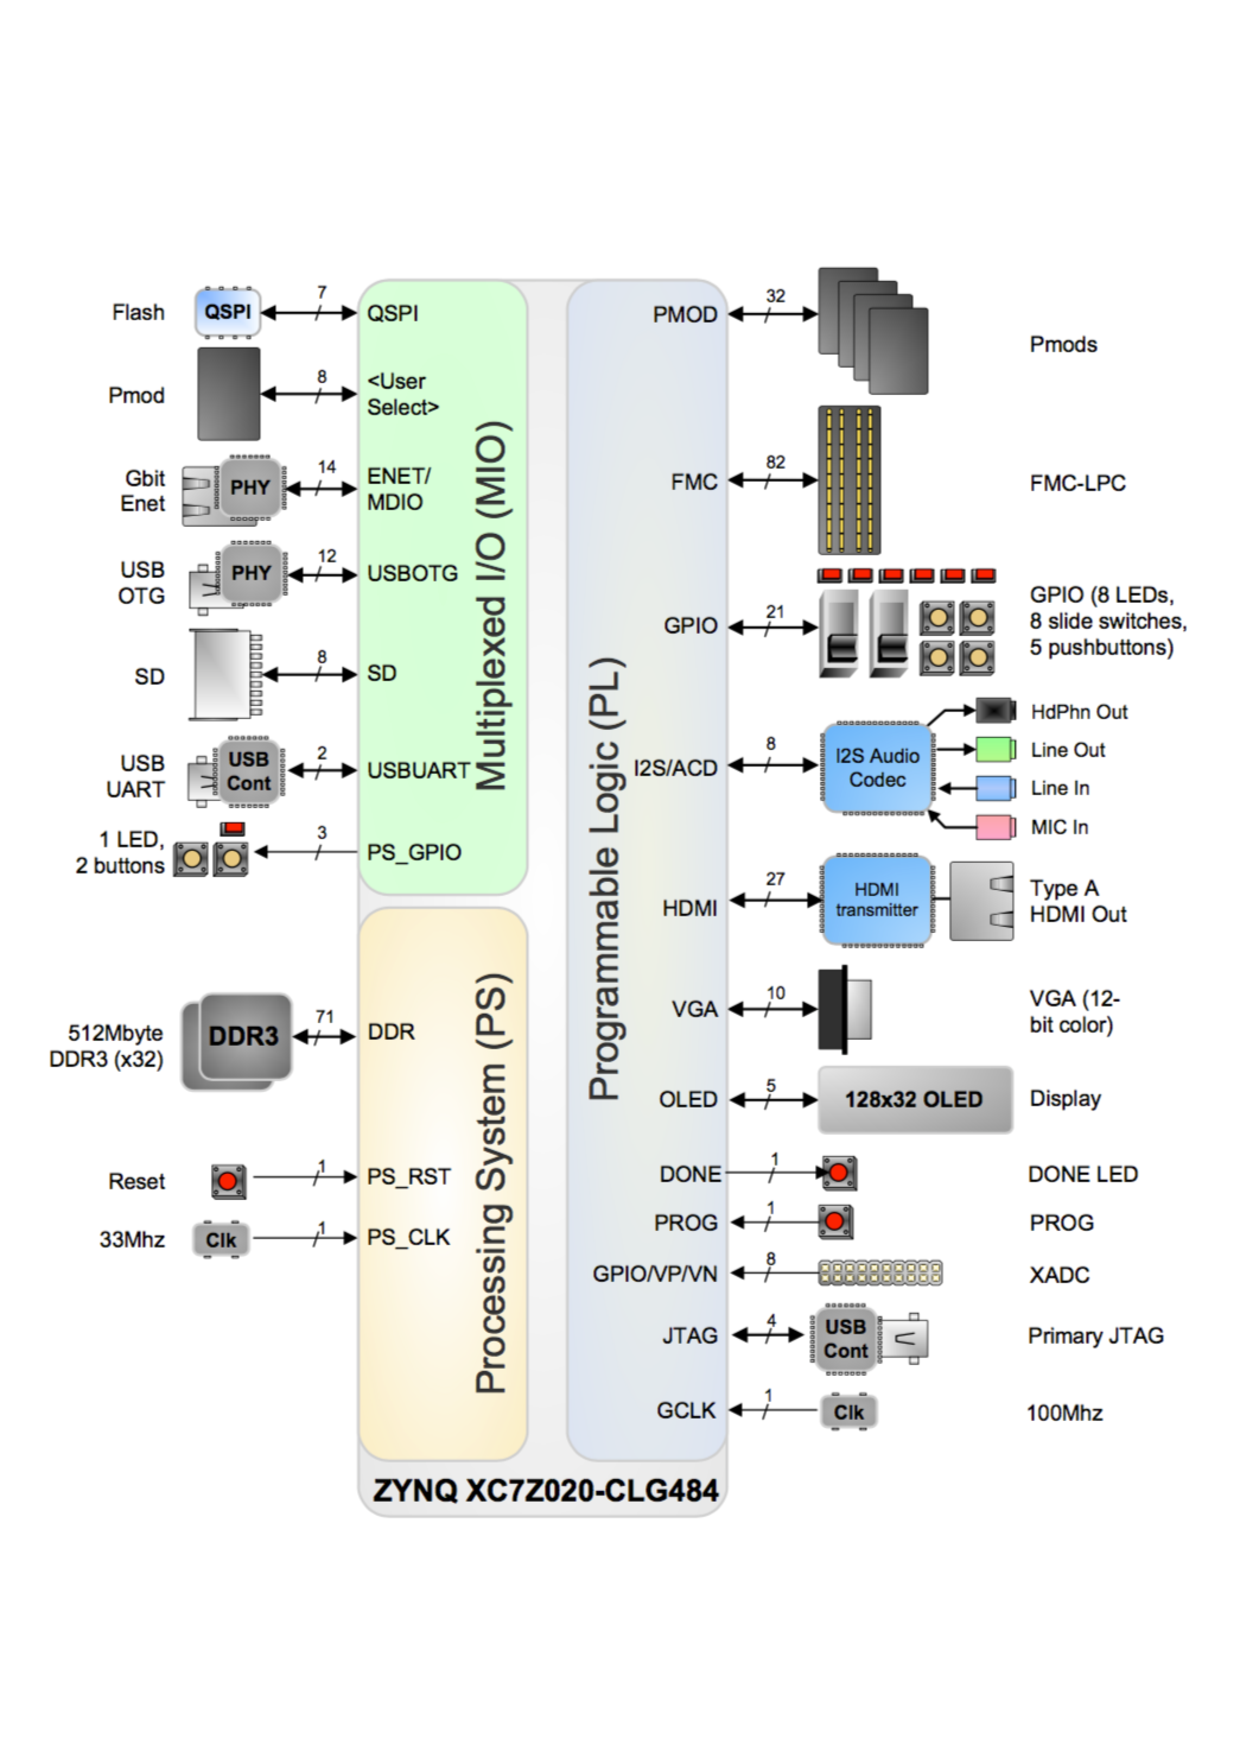
\includegraphics[width=0.6\linewidth]{images/zedboard_block_diagram}
	\caption{ZedBoard Blockdiagramm \cite[3]{manual:zedboard}}
	\label{fig:zedboard_block_diagram}
\end{figure}

\section{DE1-SoC development kit}
\label{sec:basics_de1_soc}

Das DE1-SoC Board von Terasic ist ein Eintwicklungs- und Evaluationsboard mit einem verbauten Cyclone V \gls{FPGA}-\gls{SoC}.

Wenn man das in \cref{fig:de1_soc_block_diagram} abgebildete Blockdiagramm betrachtet und mit dem Blockdiagramm des ZedBoard in \cref{fig:zedboard_block_diagram} vergleicht, so fallen starke Ähnlichkeiten auf. Diese sind darin begründet, dass bei beiden \glspl{FPGA} ein ähnliches Konzebt verfolgt wird, bei dem sowohl ein \gls{ARM}-Prozessor als auch ein \gls{FPGA} mit Peripherie zur Verfügung gestellt wird. Diese Architektur wird in der Altera-Terminologie \enquote{SoC FPGA} bzw. \enquote{SoCFPGA} genannt \cite[1]{manual:socfpga}. 

\begin{figure}[!htbp]
	\centering
	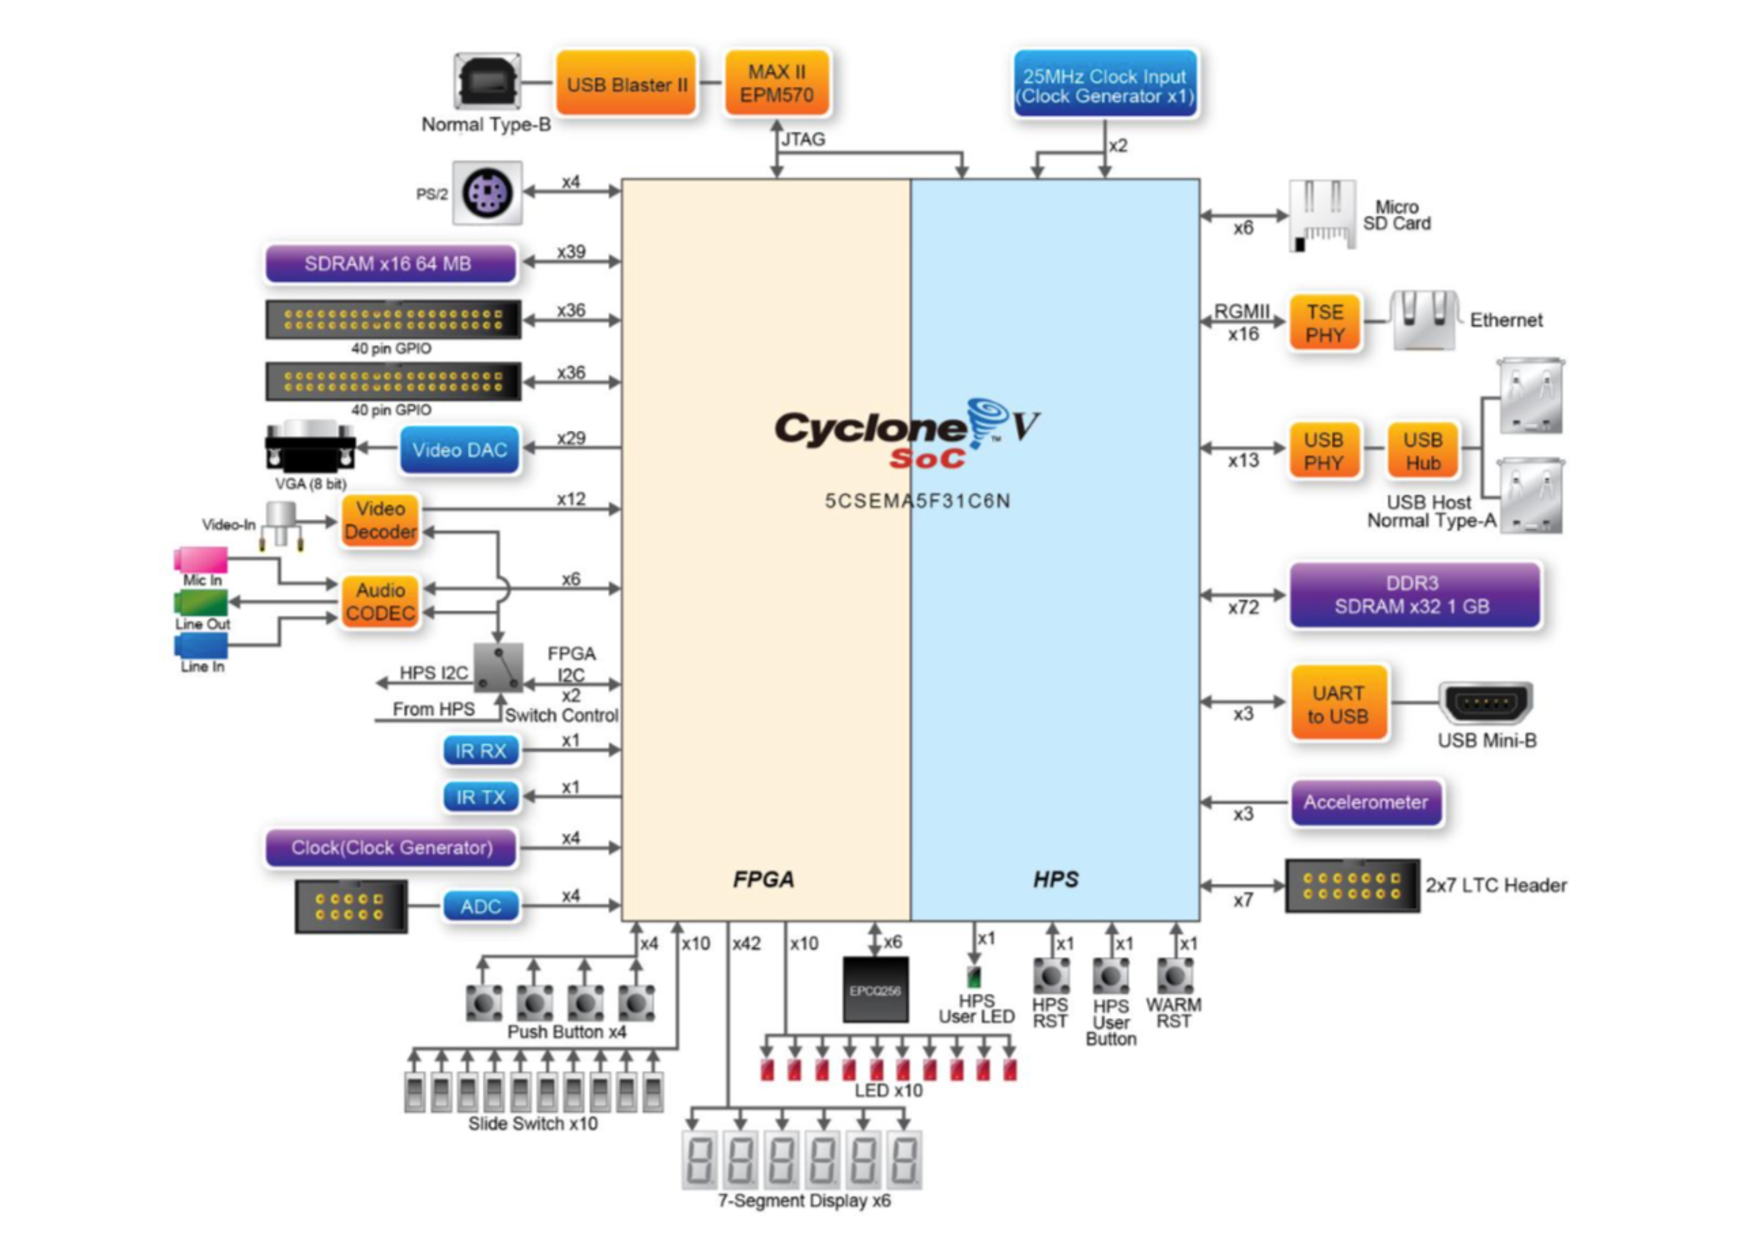
\includegraphics[width=0.7\linewidth]{images/de1_soc_block_diagram}
	\caption{DE1-SoC Blockdiagramm \cite[9]{manual:de1soc}}
	\label{fig:de1_soc_block_diagram}
\end{figure}

Auf dem DE1-SoC-Board stehen folgende Komponenten zur Verfügung \cite{manual:de1soc}:
\begin{easylist}[itemize]
	& \gls{FPGA}
	&& Altera Cyclone\textregistered V SE \gls{FPGA}
	&& \SI{64}{\mega\byte} SDRAM (\SI{16}{bit} Datenbus)
	&& 4 Taster
	&& 10 Schalter
	&& 10 rote LEDs
	&& 6 7-Segment-Anzeigen
	&& 4 \SI{50}{\mega\hertz} Oszillatoren
	&& \SI{24}{bit} Audio-CODEC mit Line- und Mikrofoneingängen und Line-Ausgang
	&& VGA DAC mit VGA-Ausgang
	&& TV Decoder (NTSC/PAL/SECAM) und TV-Eingang
	&& PS/2 Maus-/Tastaturanschluss
	&& Infrarot Sender/Empfänger
	&& Zwei 40-Pin GPIO-Leisten
	
	& \gls{HPS}
	&& \SI{800}{\mega\hertz} Dual-core ARM Cortex-A9 MPCore Prozessor
	&& \SI{1}{\giga\byte} DDR3 SDRAM (\SI{32}{bit} Datenbus)
	&& 1 Gigabit Ethernet PHY mit einem RJ45 Anschluss
	&& 2-Port USB Host, normal Type-A USB Stecker
	&& Micro SD-Kartenschacht
	&& Beschleunigungssensor (I2C)
	&& UART to USB, USB Mini-B Stecker
	&& Warm-Reset und Cold-Reset-Taster
	&& Ein benutzerdefinierte Taster, eine benutzerdefinierte LED
	&& LTC 2x7 Erweiterungsstecker
\end{easylist}

In \cref{fig:de1_soc_view_layout} ist die Ober- und Unterseite des DE1-SoC-Boards mit Hervorhebung der einzelnen Komponenten abgebildet.

\begin{figure}[!htbp]
	\centering
	\begin{subfigure}{.6\textwidth}
		\centering
		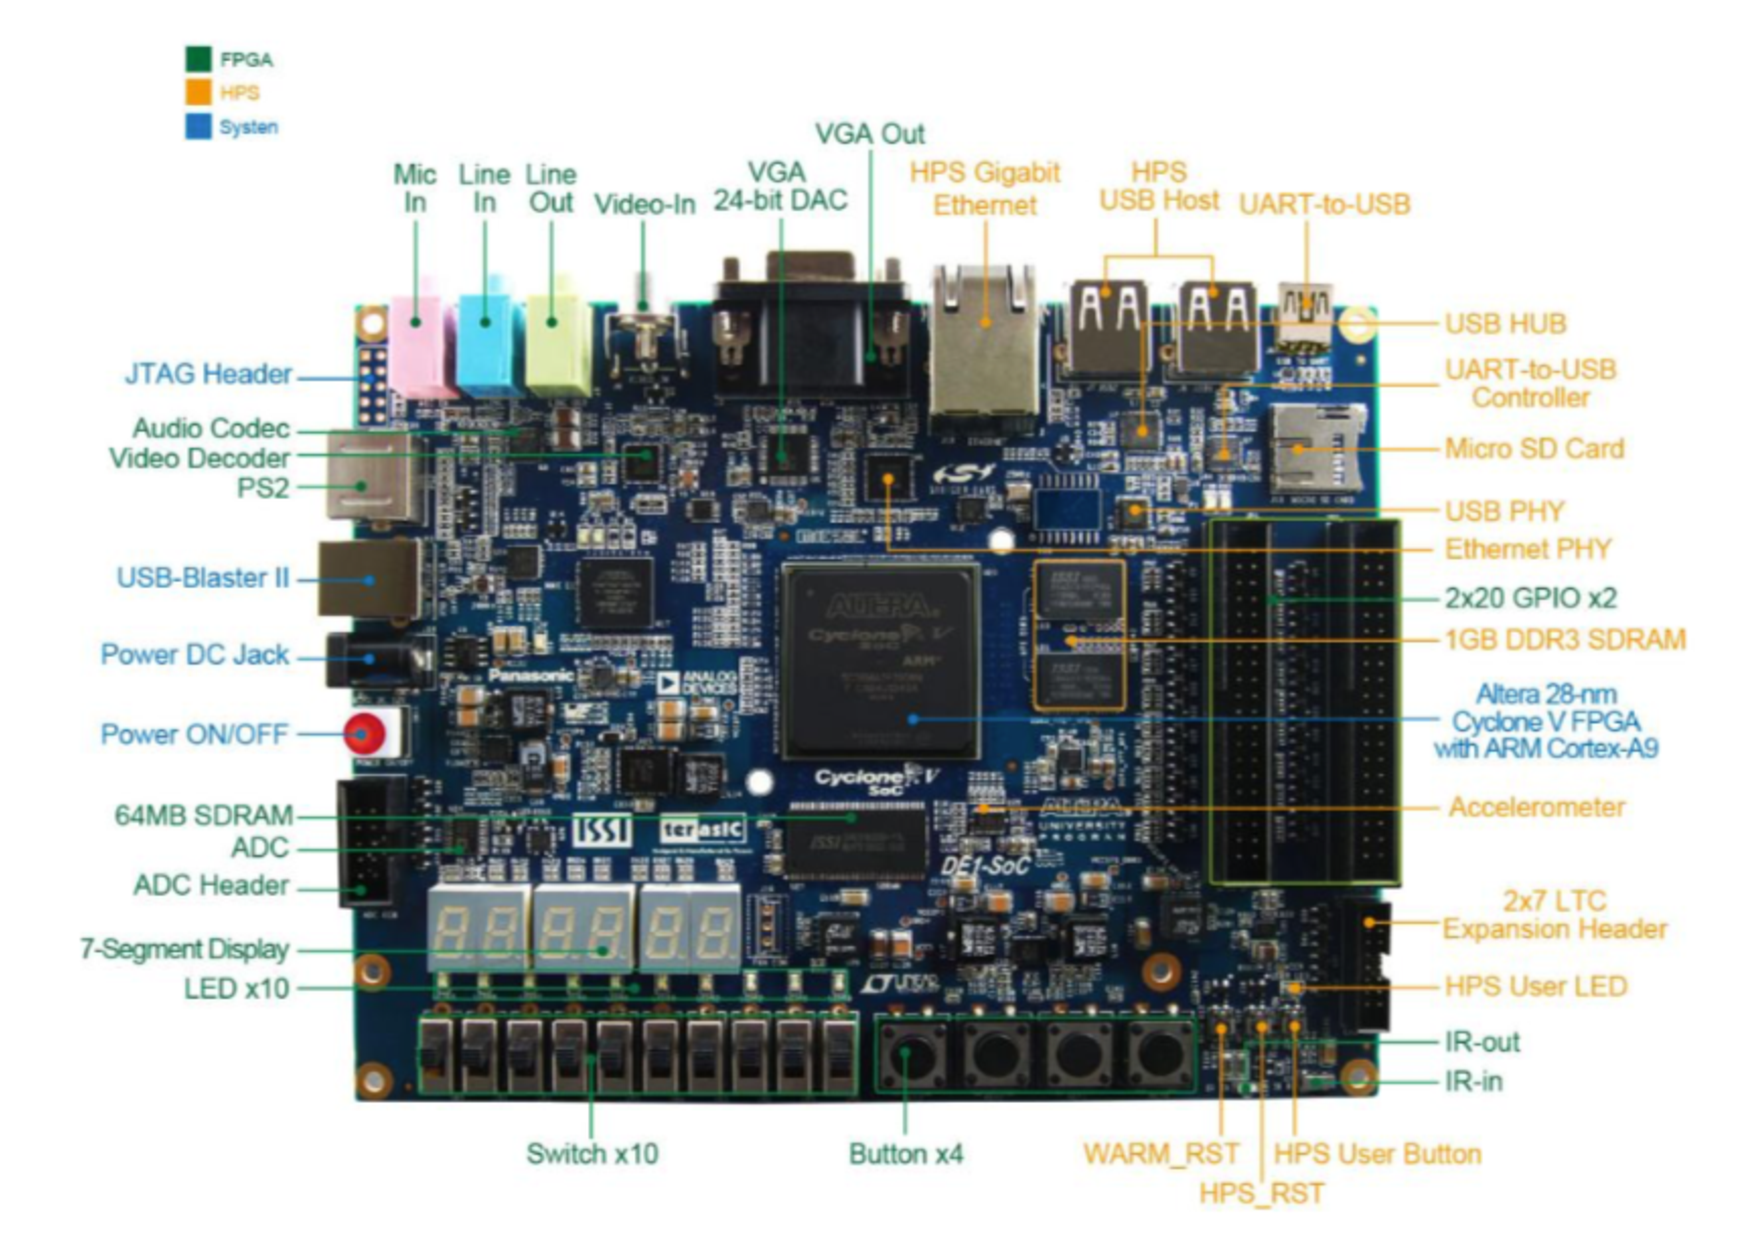
\includegraphics[width=.9\linewidth]{images/de1_soc_view_top}
		\caption{Oberseite}
		\label{fig:de1_soc_view_top}
	\end{subfigure}%
	\begin{subfigure}{.4\textwidth}
		\centering
		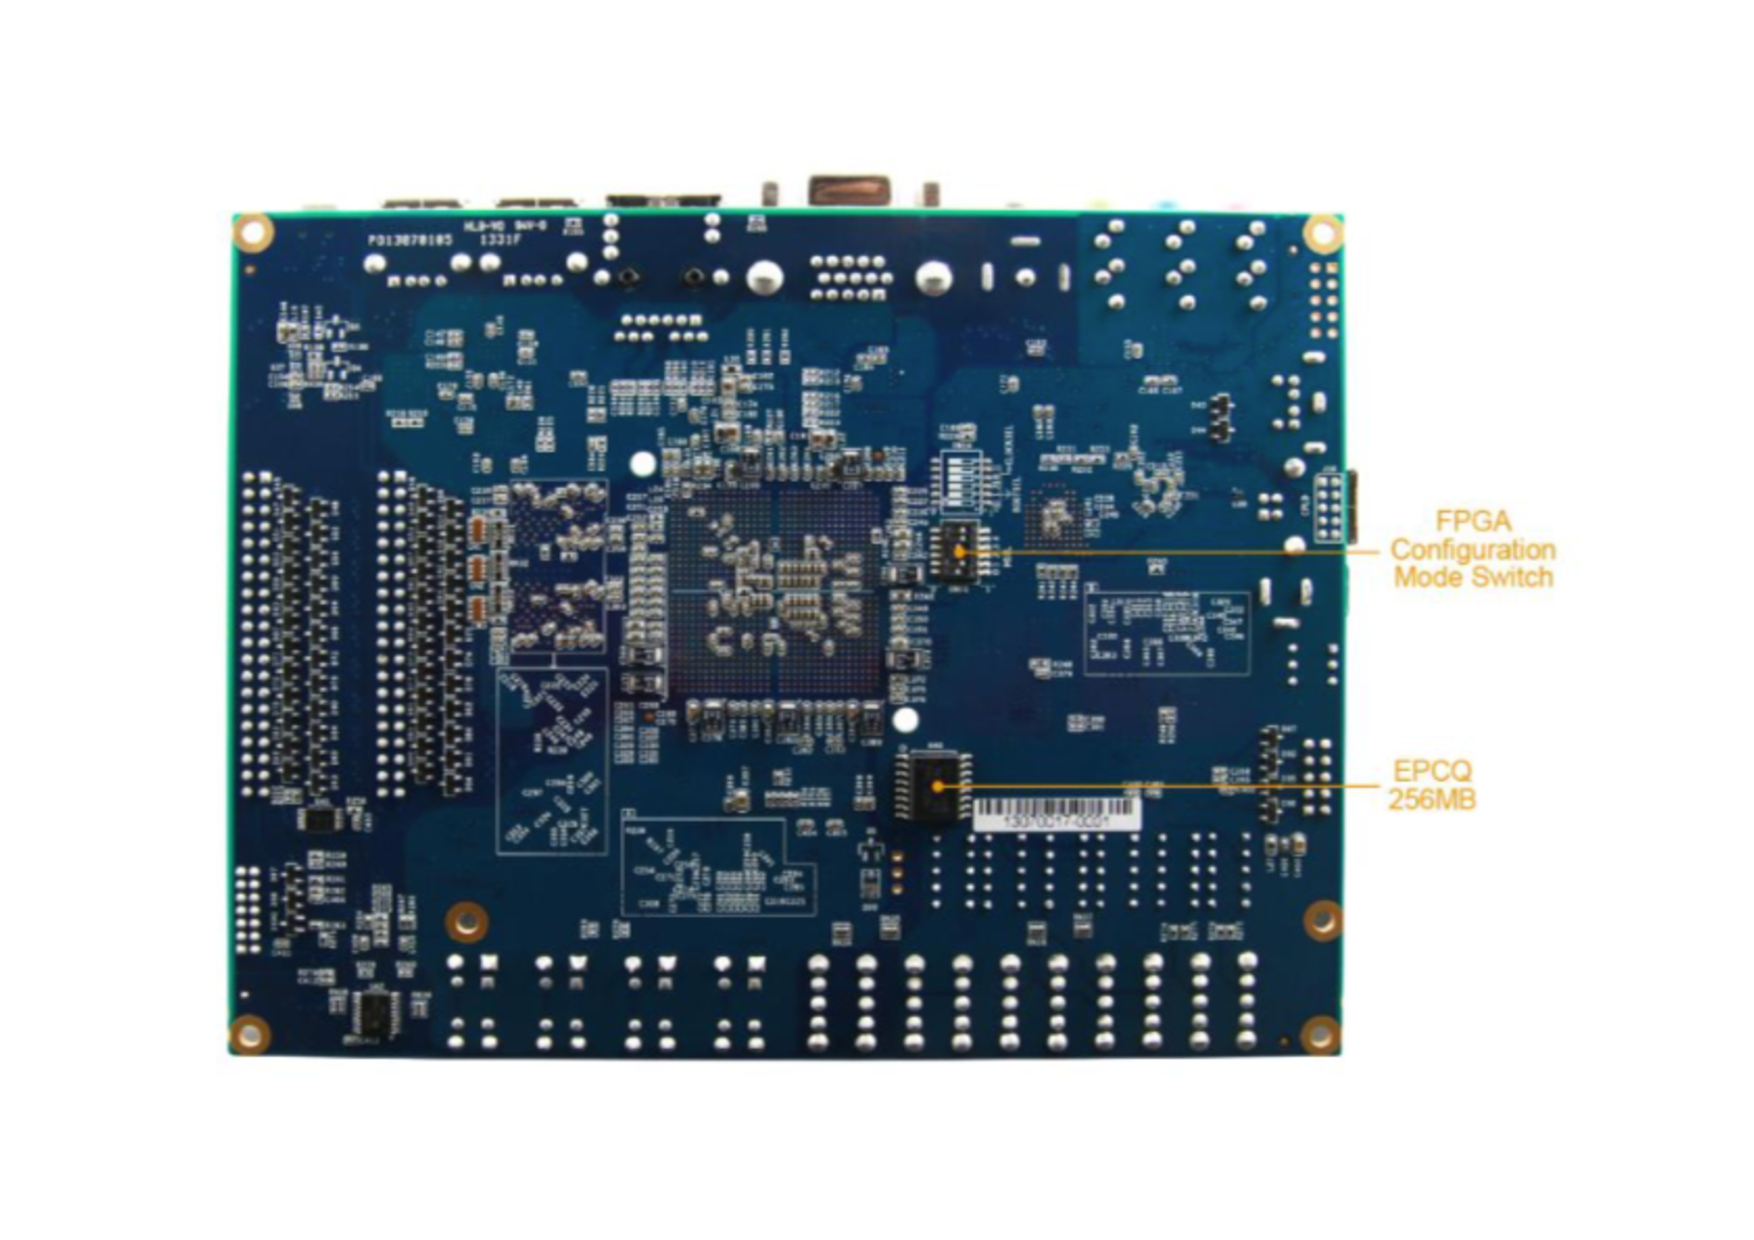
\includegraphics[width=.9\linewidth]{images/de1_soc_view_bottom}
		\caption{Unterseite}
		\label{fig:de1_soc_view_bottom}
	\end{subfigure}
	\caption{DE1-SoC Board-Layout \cite[7]{manual:de1soc}}
	\label{fig:de1_soc_view_layout}
\end{figure}

Zu beachten ist die Einstellung des \enquote{FPGA Configuration Mode Switch} auf der Unterseite des Boards (siehe \cref{fig:de1_soc_msel_switch}). Davon hängt der Konfigurationszeitpunkt des \gls{FPGA} und Programmierbarkeit des \gls{FPGA} zur Laufzeit.

\begin{figure}[!htbp]
	\centering
	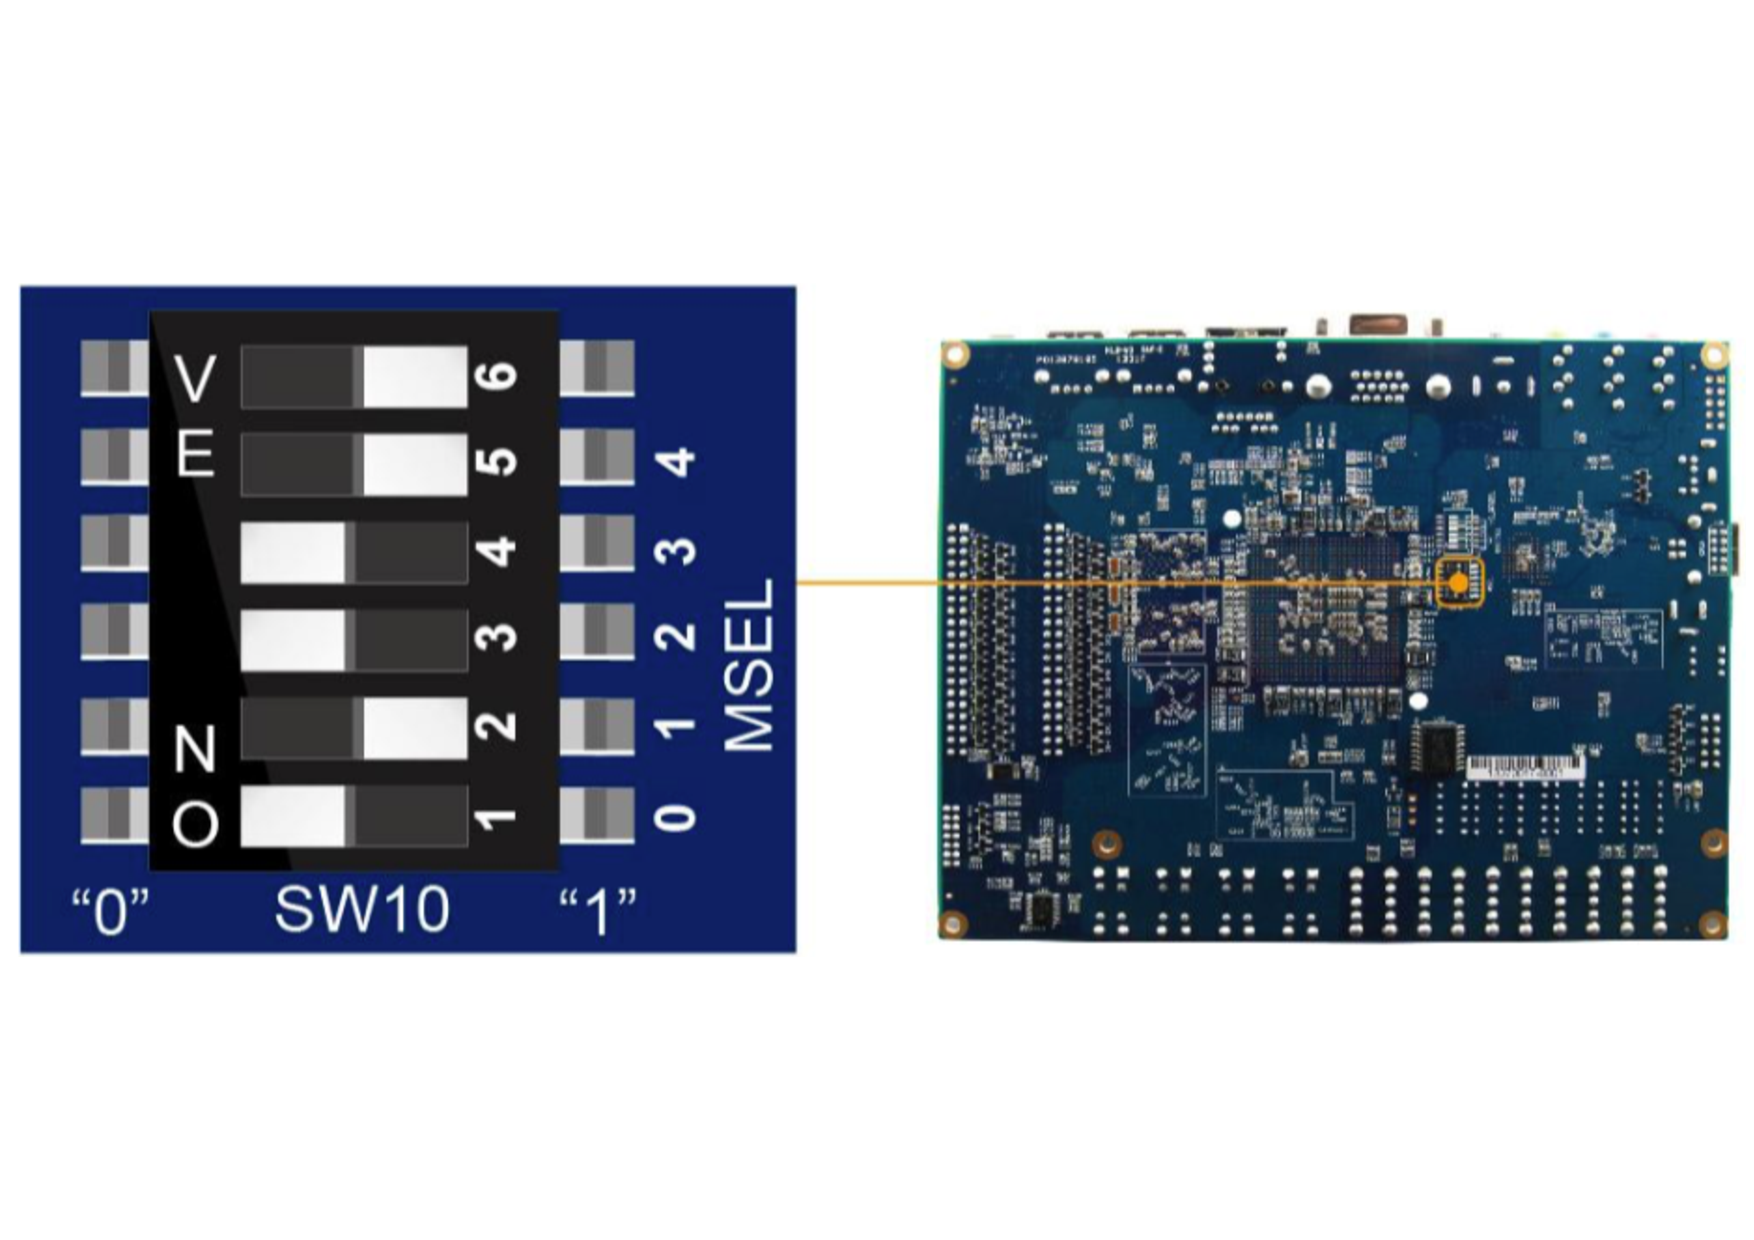
\includegraphics[width=0.7\linewidth]{images/MSEL_config}
	\caption{FPGA Configuration Mode Switch \cite[12]{manual:de1soc}}
	\label{fig:de1_soc_msel_switch}
\end{figure}

\begin{table}[!htbp]
	\bigskip
	\centering
	\begin{tabular}{| l | l | l | }
		\hline
		\textbf{MSEL[4:0]} & \textbf{Konfiguration} & \textbf{FPGA-Konfigurationsquelle} \\
		\hline
		\texttt{10010} & AS & EPCS (Voreinstellung) \\
		\hline
		\texttt{01010} & FPPx32 & \gls{HPS}-Software (Linux) \\
		\hline
		\texttt{00000} & FPPx16 & \gls{HPS}-Software (U-Boot, Abbild auf der SD-Karte) \\
		\hline
	\end{tabular}
	
	\caption{FPGA Konfigurationsmodi \cite[13]{manual:de1soc}}
	\label{tab:de1_soc_msel}
\end{table}

\alertwarning{Eine häufige Fehlerquelle ist eine spiegelverkehrte Einstellung der Konfigurationsschalter, wenn das Board so gehalten wird, dass die PCB-Legenden auf der Unterseite des Boards von links nach rechts gelesen werden können. Die Pin-Belegung ist nicht intuitiv, das MSB befindet sich \textbf{rechts}, und logisch \enquote{1} ist \textbf{unten}}

\section{Quartus Prime 18.0}
Um Hardware für einen \gls{FPGA} entwickeln zu können, bedarf es einer passenden Entwicklungsumgebung. Da dem verwendeten Board ein Altera/Intel \gls{FPGA} zugrundeliegt, wird die Entwicklungsumgebung \enquote{Quartus Prime} verwendet. Diese ist nach einer Registrierung kostenfrei in der Version \enquote{Quartus Prime Lite Edition 18.0} im Downloadportal\footnote{\url{http://fpgasoftware.intel.com/?edition=lite}} von Intel verfügbar. 

In der Entwicklungsumgebung sind mehrere Anwendungen (siehe \cref{fig:quartus_apps}) enthalten, die in dieser Bachelorarbeit verwendet werden:
\begin{easylist}[itemize]
	& Quartus Prime: Wird zur \gls{HDL}-Synthese verwendet
	& Platform Designer: Grafisches \gls{SoC}-Designwerkzeug
	& Signal Tap: Synthetisierbarer Logikanalysator mit grafischer Benutzeroberfläche zur Signaldefinition und Auswertung
	& Modelsim: \gls{HDL}-Simulator
\end{easylist}

\begin{figure}[!htbp]
	\centering
	\begin{subfigure}[b]{0.475\textwidth}
		\centering
		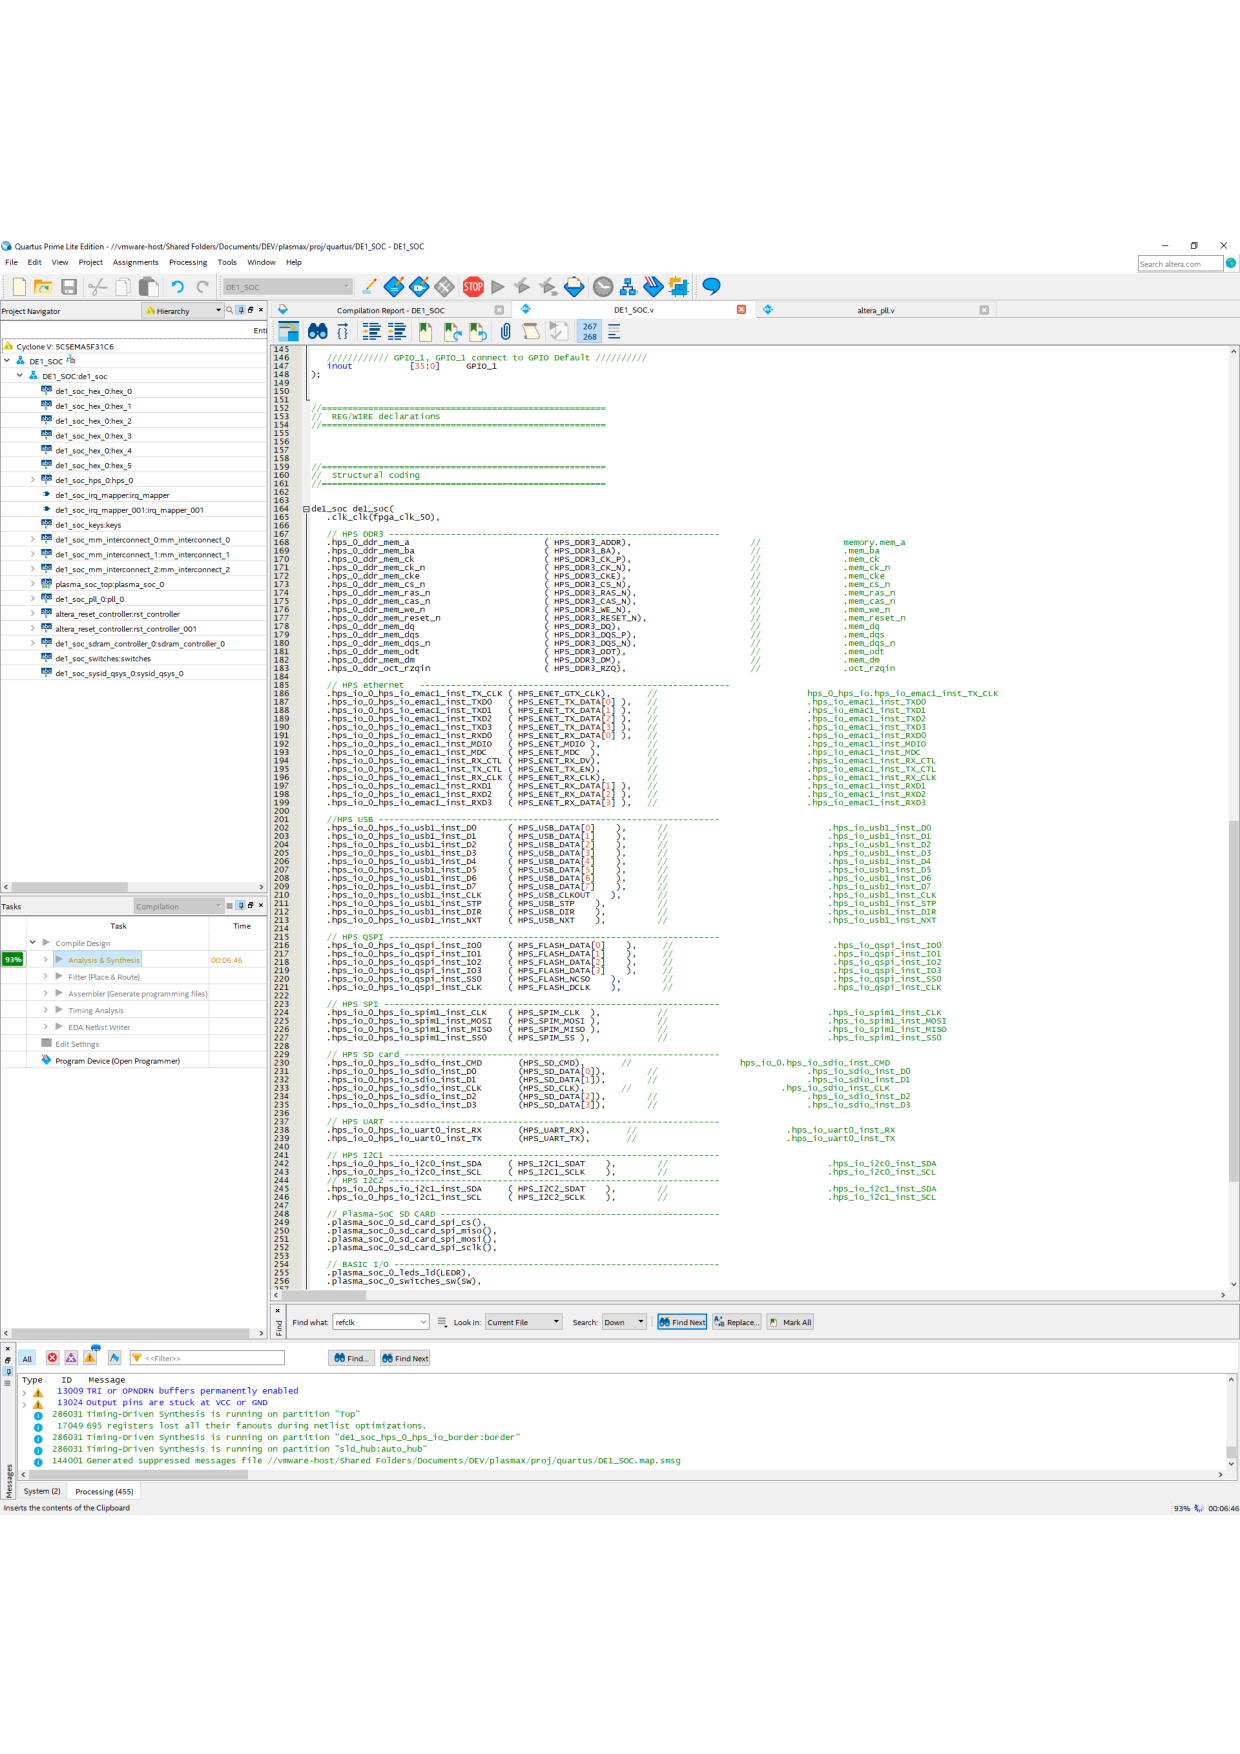
\includegraphics[width=\textwidth]{images/quartus_mainwindow}
		\caption{Quartus}
		\label{fig:quartus_mainwindow}
	\end{subfigure}
	\hfill
	\begin{subfigure}[b]{0.475\textwidth}  
		\centering 
		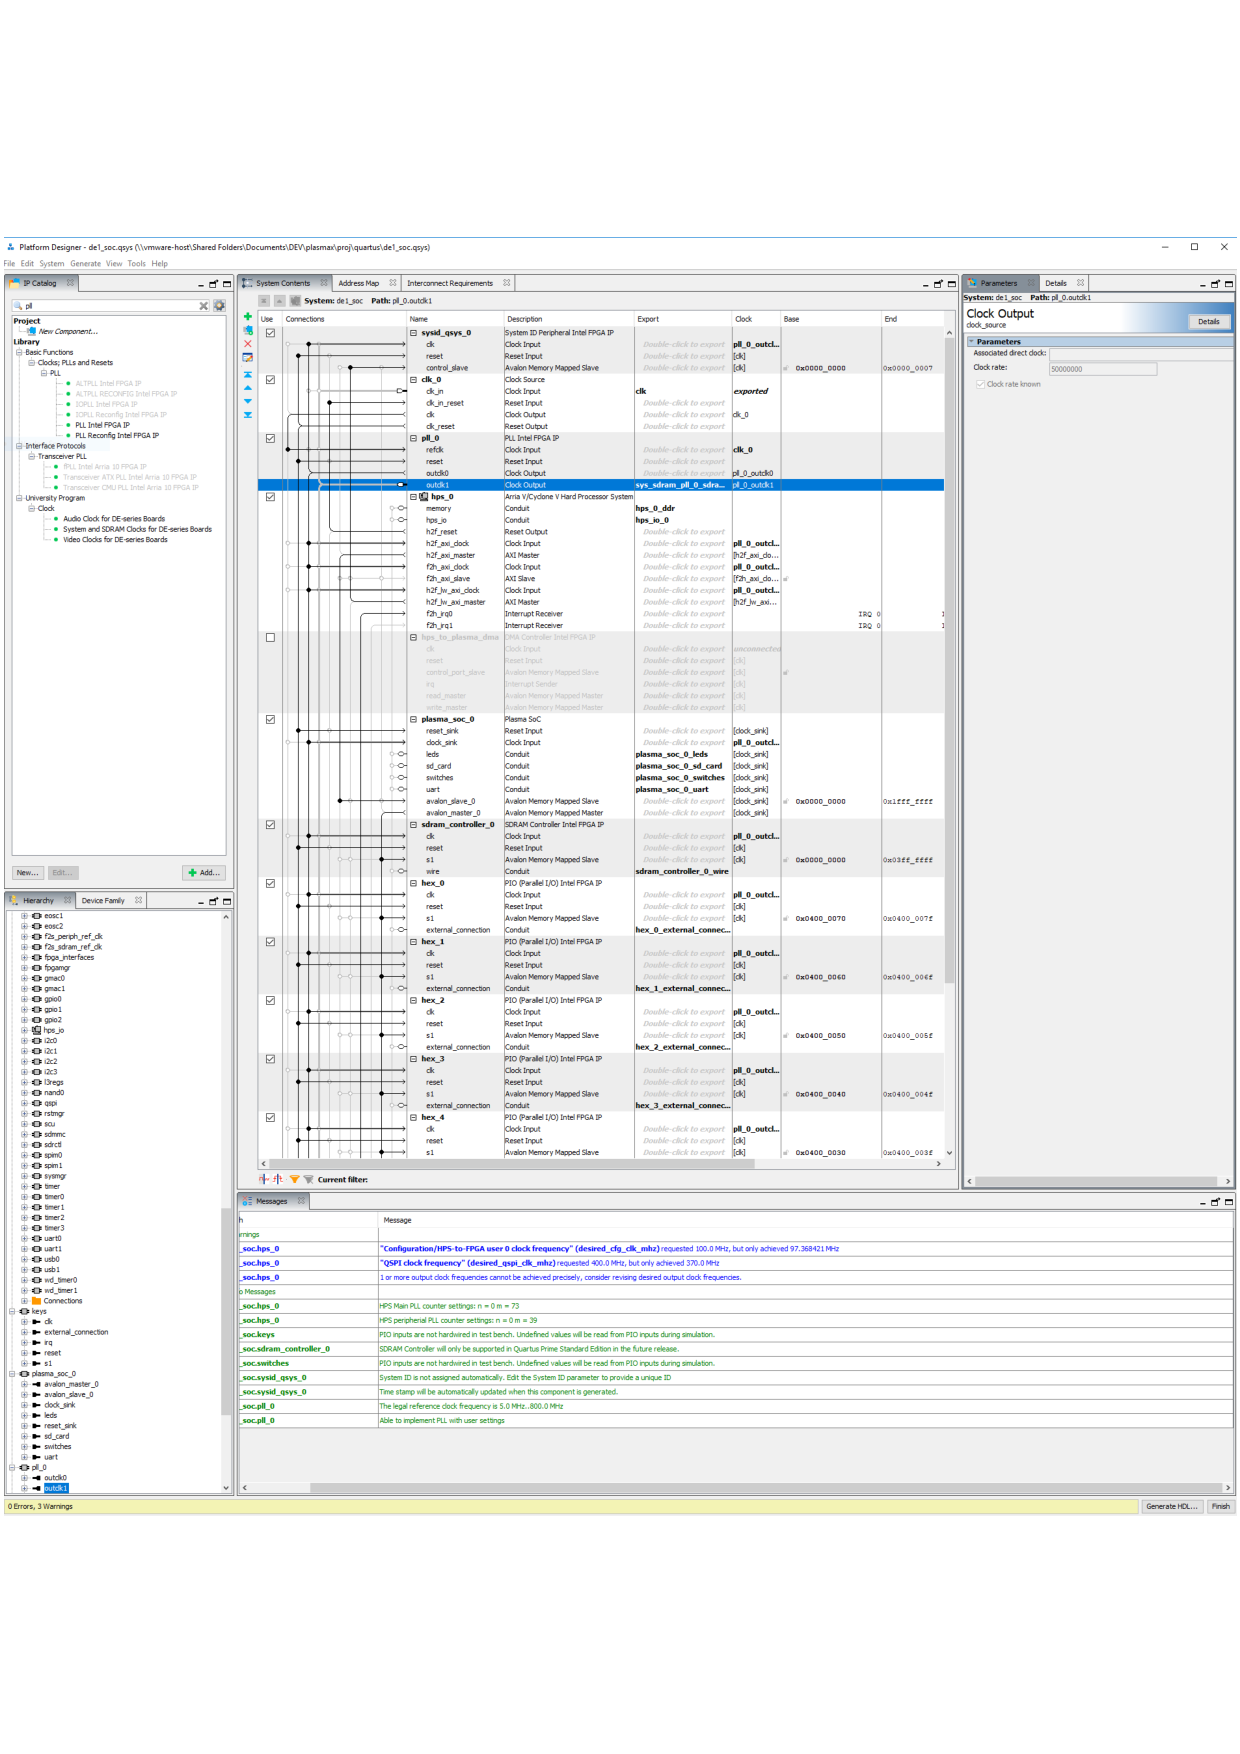
\includegraphics[width=\textwidth]{images/quartus_platformdesigner}
		\caption{Platform Designer}
		\label{fig:quartus_platformdesigner}
	\end{subfigure}
	\vskip\baselineskip
	
	\begin{subfigure}[b]{0.475\textwidth}   
		\centering 		
		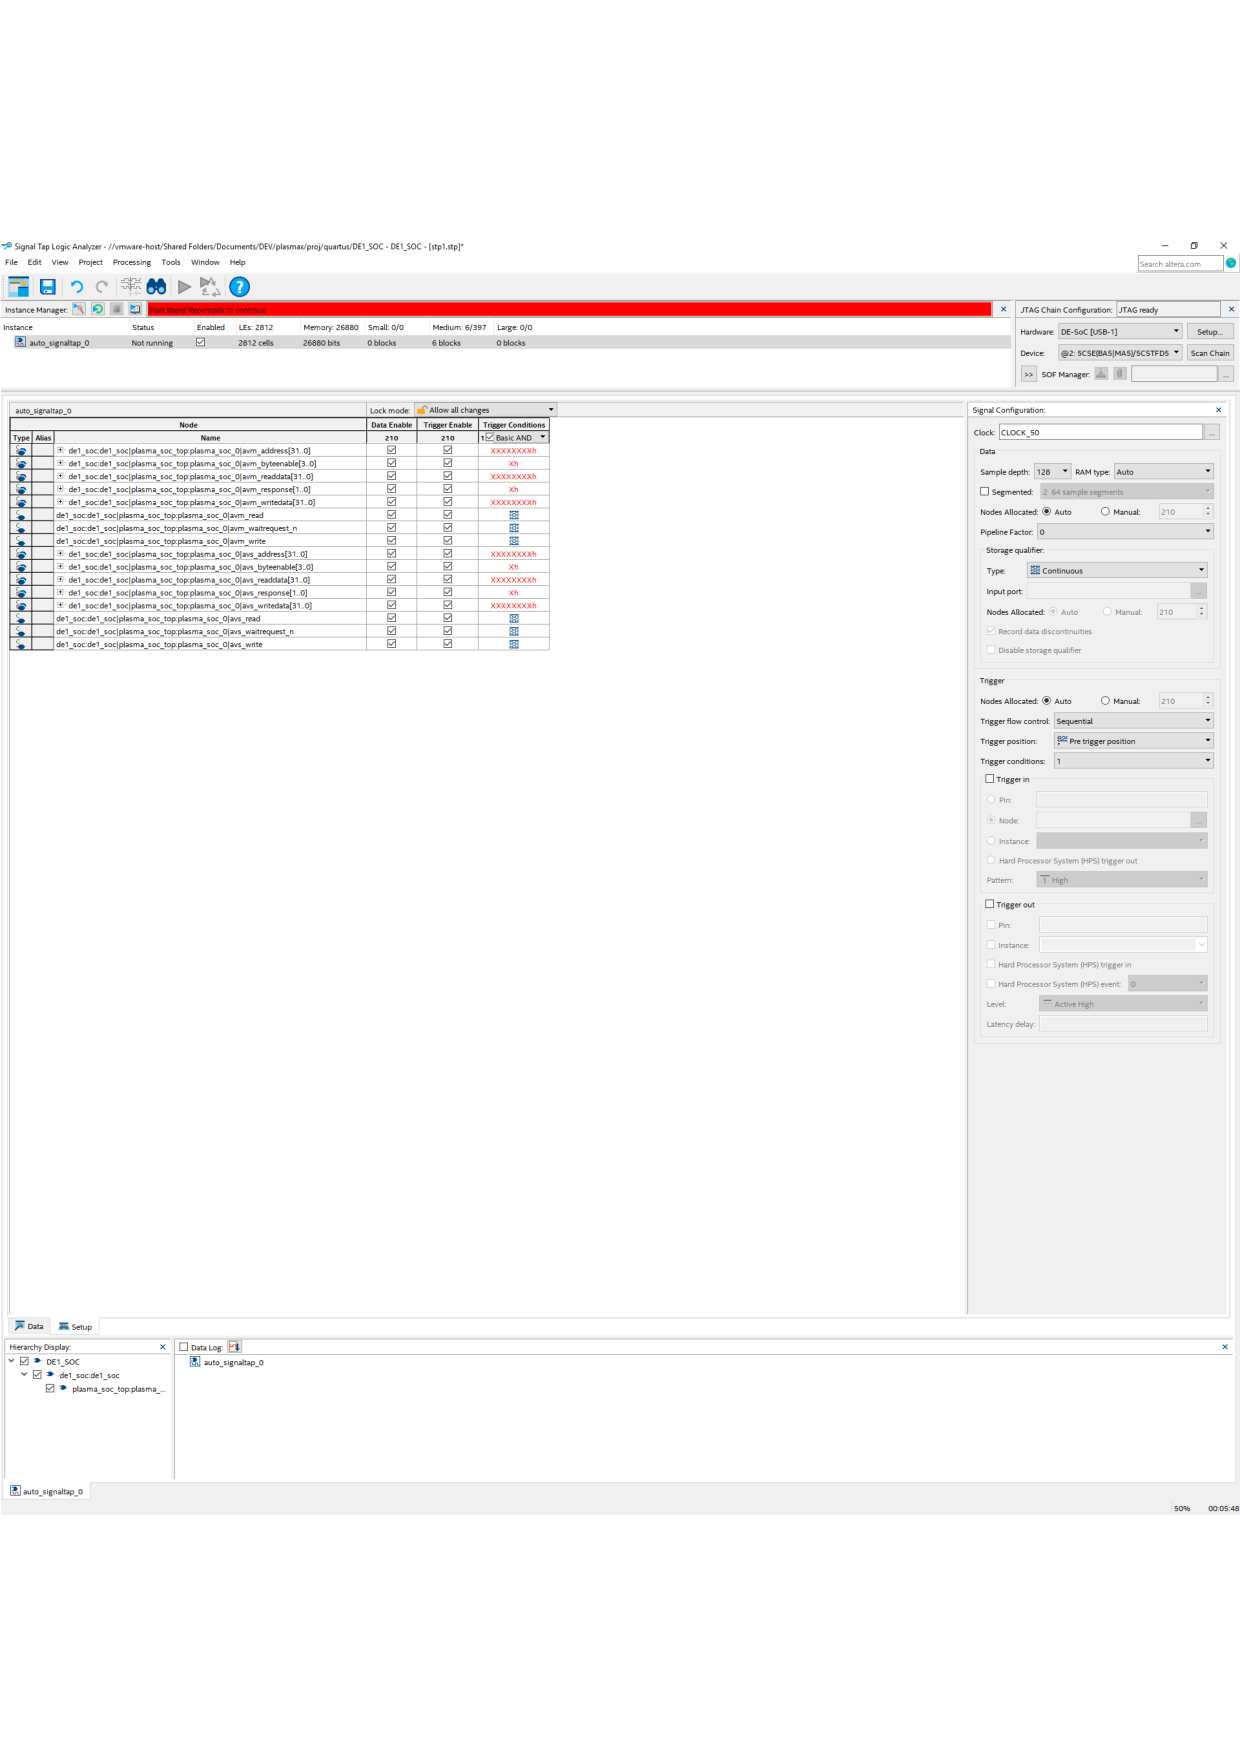
\includegraphics[width=\textwidth]{images/signaltap}
		\caption{Signal Tap}
		\label{fig:signaltap}
	\end{subfigure}
	\quad
	\begin{subfigure}[b]{0.475\textwidth}   
		\centering 
		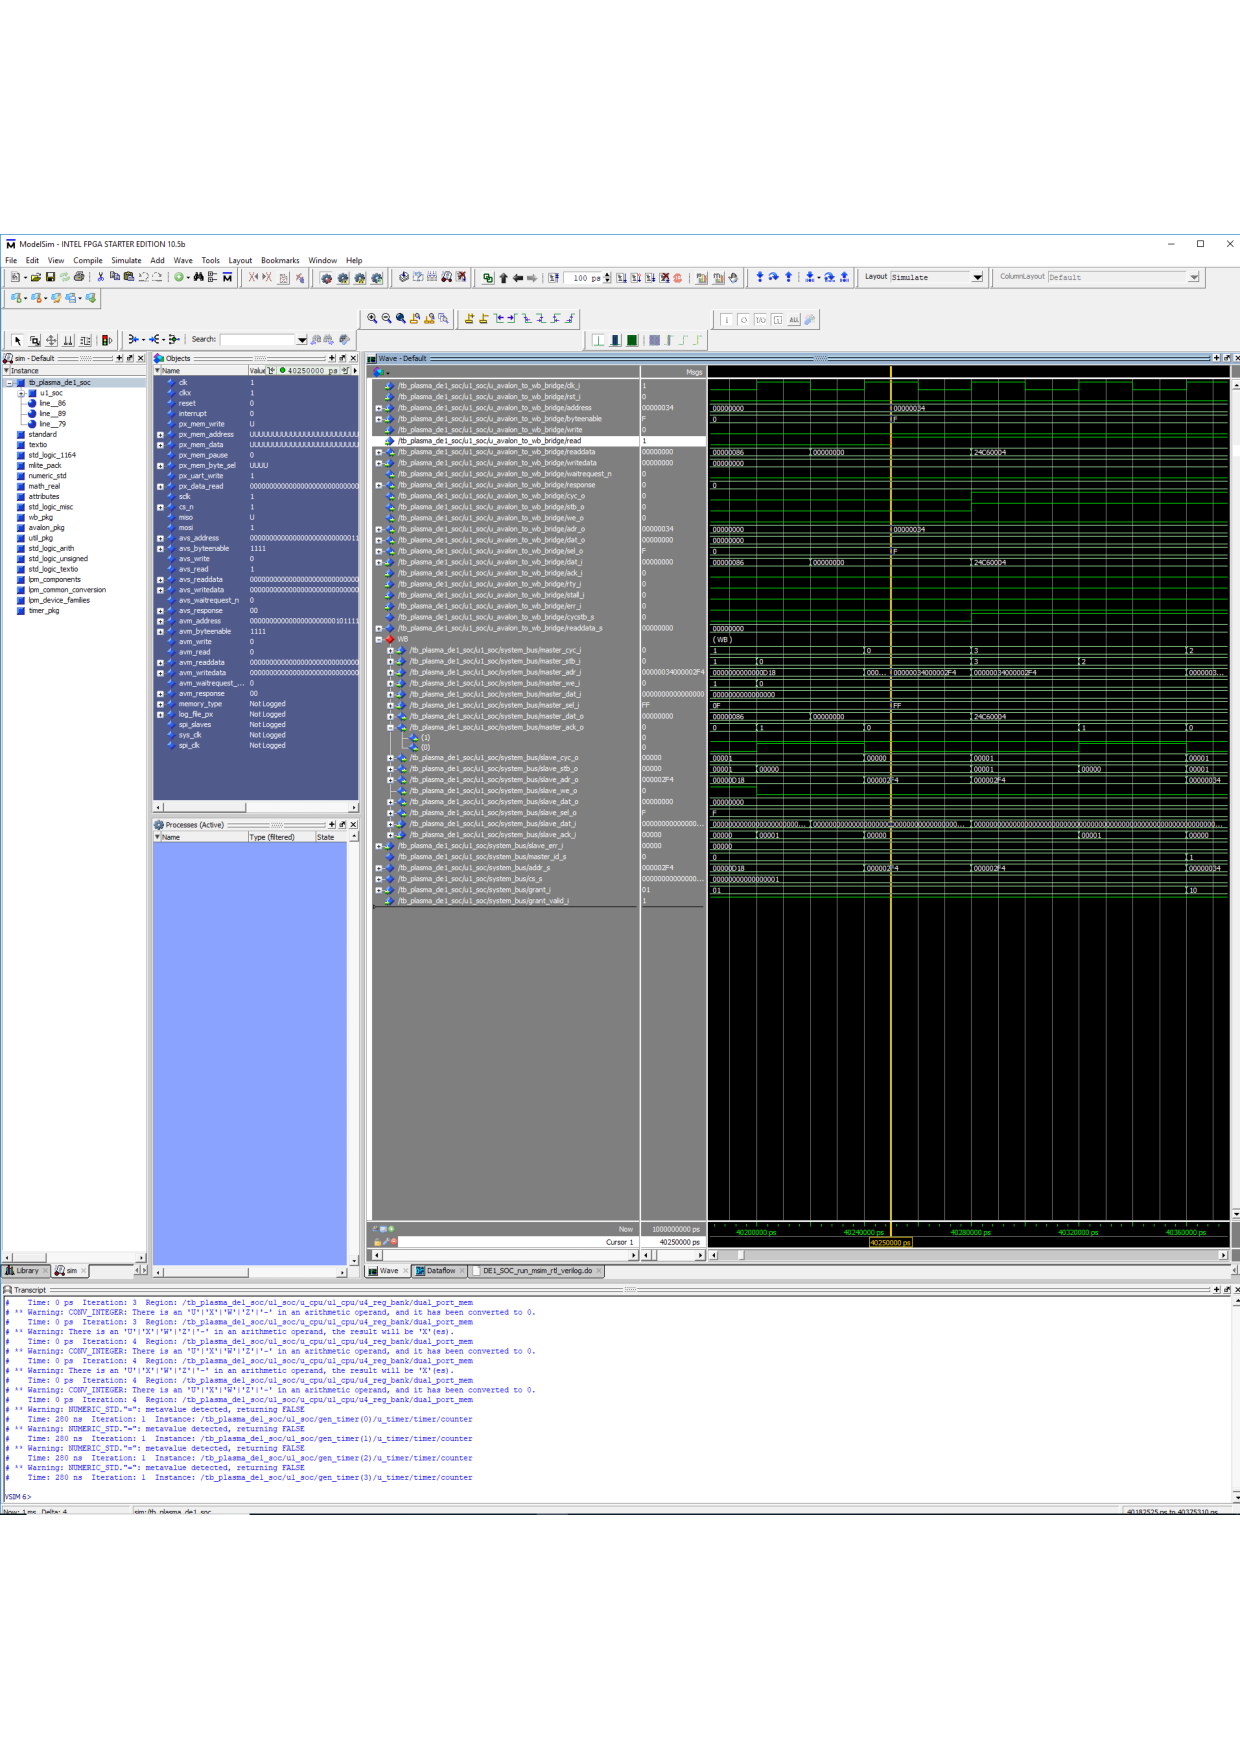
\includegraphics[width=\textwidth]{images/modelsim}
		\caption{Mentor Graphics Modelsim}
		\label{fig:modelsim}
	\end{subfigure}
	\caption{Quartus Anwendungen}
	\label{fig:quartus_apps}
\end{figure}

\section{SoC FPGA Embedded Development Suite (SoC EDS)}
Um Software für \gls{ARM}-basierte eingebettete Systeme entwickeln zu können, wird eine weitere Entwicklungsumgebung benötigt.
 
Genau so wie Quartus Prime ist SoC EDS nach einer Registrierung kostenfrei im Downloadportal\footnote{\url{http://fpgasoftware.intel.com/soceds/18.0/?edition=standard}} von Intel verfügbar. 

Folgende Anwendungen werden in dieser Bachelorarbeit verwendet:
\begin{easylist}[itemize]
	& Cross-Compiler für die \gls{ARM}-Architektur
	& Devicetree Compiler
	& \gls{BSP}-Editor
\end{easylist}
	\chapter{Grundlagen}
\label{cha:basics}

In diesem Kapitel wird zunächst auf die Motivation für ein \gls{SoC} und dessen Grundaufbau eingegangen. In diesem Zusammenhang wird auf die Bus-Architekturen \enquote{Wishbone} und \enquote{Avalon} eingegangen. Danach wird das Plasma-System von Steve Rhoads, sowie die Entwicklungs- und Evaluationsboards ZedBoard \cite{manual:zedboard} von Digilent und DE1-SoC \cite{manual:de1soc} von Terasic vorgestellt.

\section{System-On-Chip}

Der Begriff \gls{SoC} wurde durch die Integration eines gesamten Systems (Prozessor, Speicher und Peripherie) auf einem einzigen Chip geprägt.
Die \glspl{SoC} sind aus modernen Geräten nicht wegzudenken. Ein prägnantes Beispiel hierfür ist ein Smartphone: auf einem einzigen Chip sind beispielsweise eine \gls{CPU}, \gls{GPU}, \gls{GSM}-Modem, ein Display-Controller sowie der Kamera-Controller samt einem \gls{DSP} zur Bildverarbeitung integriert. Moderne Medizin-, Automobil-, Avionik-, Raumfahrt- und Militär-Systeme wären ohne \glspl{SoC} nicht möglich. Doch auch banal erscheinende Geräte wie Küchengeräte und sogar die Heimbeleuchtung (\gls{IoT} und Smart-Home) profitieren von der zunehmenden Miniaturisierung und den Einsatzmöglichkeiten der \glspl{SoC}. 

Der Entwurf eines \gls{SoC} ist mit einem sehr hohen Zeit- und Arbeitsaufwand verbunden. Je komplexer das System, desto aufwändiger wird ein von Grund auf neuer Aufbau. \cite[189]{book:embedded_sopc_design} Darum wird heutzutage, analog zur Softwareentwicklung, auf erprobte, wiederverwendbare Komponenten gesetzt. Diese sind als IP-Cores verfügbar und können in eigene Projekte integriert werden. Davon sind einige parametrisierbar und somit auf Projektbedürfnisse anpassbar. Ein IP-Core kann als high-level \gls{HDL} Code, auch Soft-Core genannt, oder auch als ein detailliertes Layout auf Transistorebene, Hard-Core genannt, ausgeliefert werden. \cite[189]{book:embedded_sopc_design} 

Ein gutes Beispiel für parametrisierbare IP-Cores ist die \gls{ARM}-CPU. ARM als Unternehmen ist kein Prozessorhersteller an sich, sondern bietet ledeglich die \gls{CPU}-Architektur als IP-Core zur Erwerb an. Ein Interessent kann diese lizenzieren, auf seine Bedürfnisse anpassen und bei einem Halbleiterfertiger in Produktion geben. Durch Kombination verschiedener auf dem Markt verfügbarer IP-Cores kann innerhalb kürzester Zeit ein neues Produkt mit einem gegenüber den Einzelkomponenten erhöhten Mehrwert entwickelt werden.

\section{Bussysteme}
\label{the:bus_system}
In vorigen Abschnitten wurden beispielhaft einige Komponenten eines \gls{SoC} genannt. Im Wesentlichen handelt es sich hierbei um eine \gls{CPU}, die mit sämtlichen domänenspezifischen Prozessoren und Peripheriegeräten bzw. Schnittstellen kommuniziert. Essentiell hierfür ist ein Bus-System, welches allen relevanten Modulen ein Kommunikationsmedium bereitstellt. Verbreitet sind standardisierte Bus-Architekturen wie AMBA, CoreConnect, Wishbone, STBus und weitere. \cite[2]{article:soc_buses} AMBA ist sehr verbreitet in der Entwicklung von \glspl{SoC} auf Basis von \gls{ARM}-Prozessoren. In dieser Arbeit wird besondere Aufmerksamkeit dem Wishbone- und Avalon-Bus gewidmet. 

\subsection{Topologien}

Unter einer Bus-Topologie versteht man die Anordnung der Master- und Slavegeräte zueinander. Je nach Topologie muss u.U. eine Arbitrierung vorgenommen werden, um Ressourcen unter mehreren Teilnehmern verteilen zu können. Die nachfolgenden Abbildungen entstammen der Wishbone-Spezifikation \cite{website:wishbone_b4_spec} und sind auch auf andere Bussysteme übertragbar. 

\begin{figure}[!htbp]
	\centering
	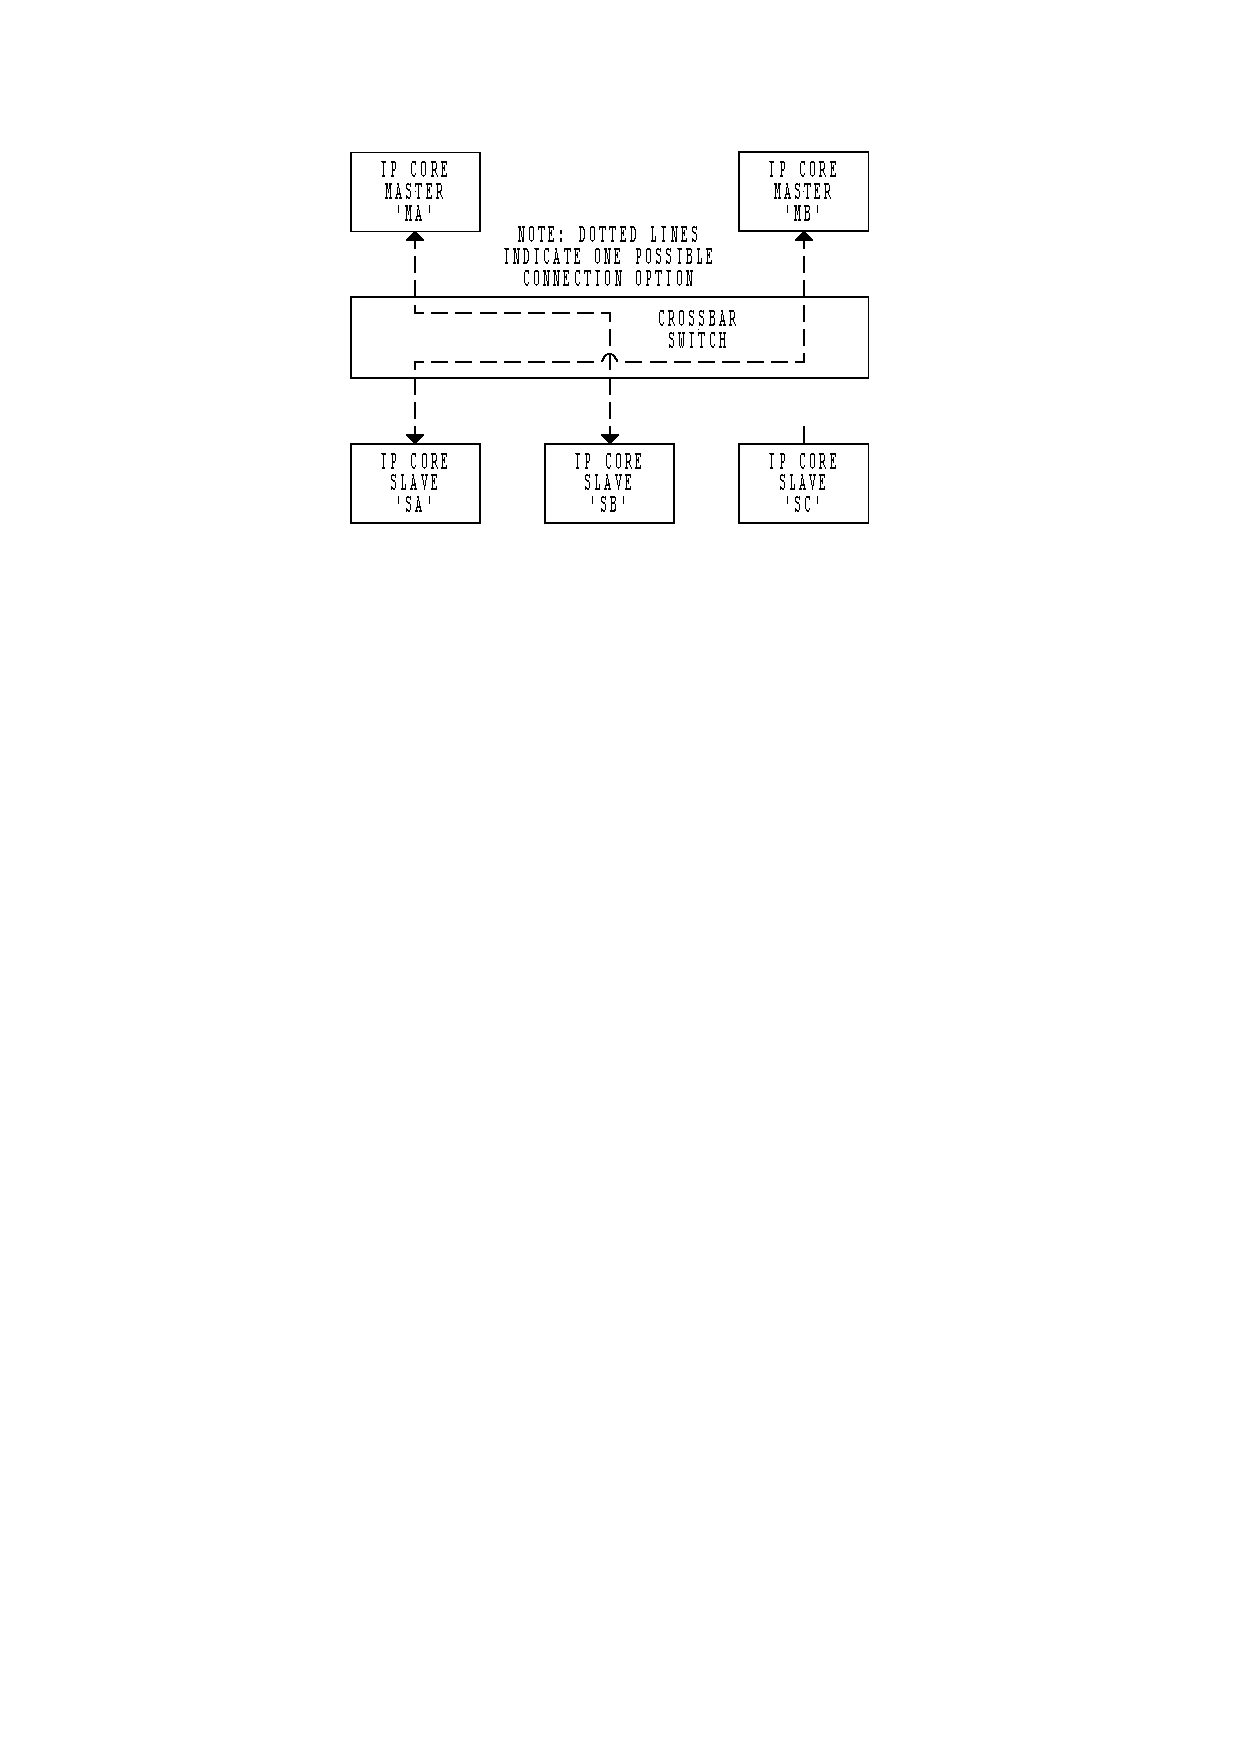
\includegraphics[width=0.6\linewidth]{images/crossbar_switch_interconnection}
	\caption{Crossbar (Switch) \cite[17]{website:wishbone_b4_spec}}
	\label{fig:crossbar_switch_intercon}
\end{figure}

In \cref{fig:crossbar_switch_intercon} ist eine Crossbar-Switch-Topologie dargestellt. In diesem Fall können mehrere Master zeitgleich eine Verbindung zu einem Slave aufnehmen. Jede Verbindung ist unabhängiig von den anderen und kann parallel betrieben werden. Durch diese Parallelität erhöht sich der Durchsatz des ganzen Systems. Diese Topologie ist geschwindigkeitsmäßig den klassischen Bussystemen überlegen. Grundsätzlich unterstützen die Crossbar Routingmechanismen dynamische Konfiguration, was zu einen zuverlässigem und konfigurierbaren Netzwerk führt. Außerdem sind die meisten Crossbar-Architekturen skalierbar, können also bei Bedarf erweitert werden. \cite[16]{website:wishbone_b4_spec}

\begin{figure}[!htbp]
	\centering
	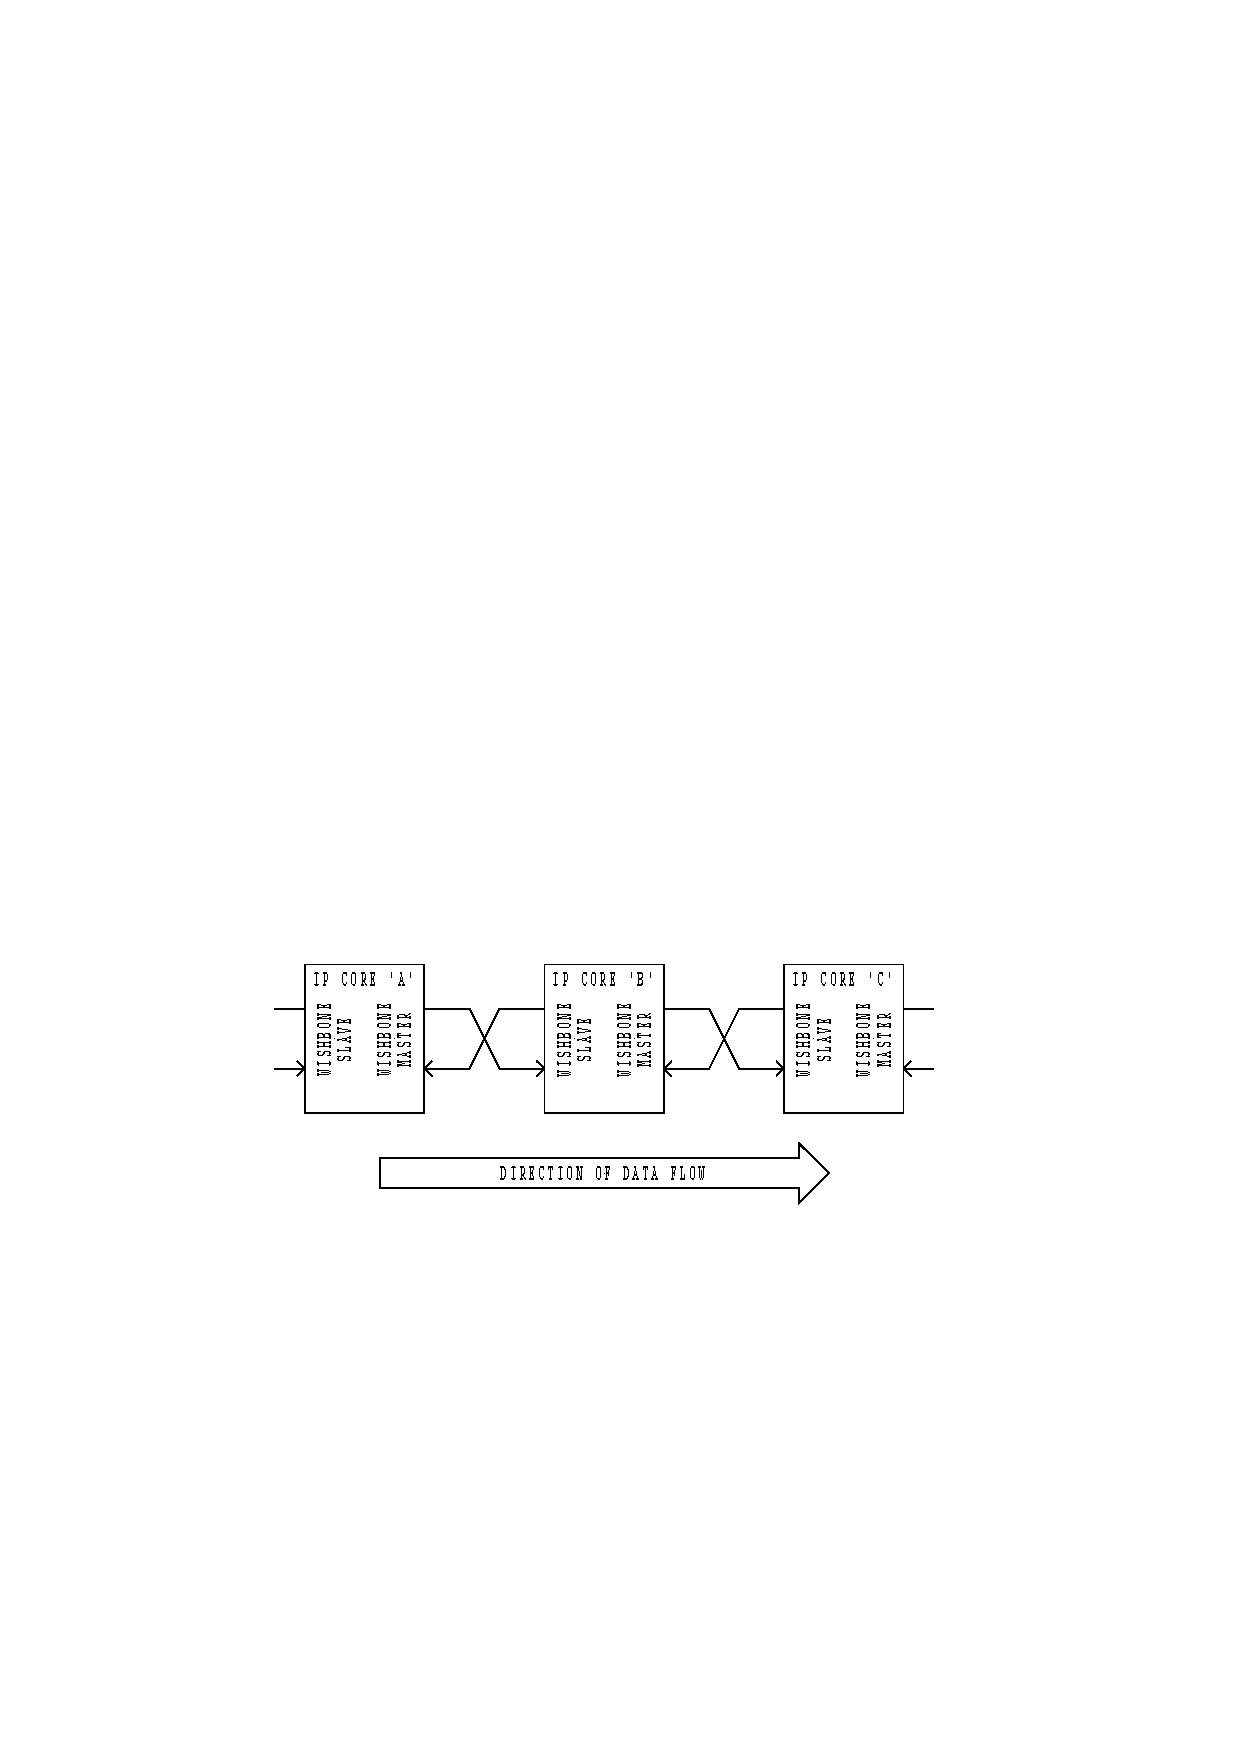
\includegraphics[width=0.9\linewidth]{images/data_flow_interconnection}
	\caption{Data flow \cite[17]{website:wishbone_b4_spec}}
	\label{fig:data_flow_intercon}
\end{figure}

In \cref{fig:data_flow_intercon} ist eine Data-Flow-Topologie dargestellt. Hierbei fließt der Datenstrom sequentiell durch einen vordefinierten Satz an IP-Cores. Data-Flow-Architekturen weisen oft eine Parallelität auf: eine oder mehrere werden Funktionen zeitgleich ausgeführt. \cite[17]{website:wishbone_b4_spec}

\begin{figure}[!htbp]
	\centering
	
\includegraphics[width=0.6\linewidth]{images/point_to_point_interconnection}
	\caption{Point to point \cite[21]{website:wishbone_b4_spec}}
	\label{fig:p2p_intercon}
\end{figure}

Eine Punkt-zu-Punkt Topologie, wie in \cref{fig:p2p_intercon} abgebildet, ist die einfachste aller Topologien mit einem einzigen Master und einem Slave.\cite[20]{website:wishbone_b4_spec}

\begin{figure}[!htbp]
	\centering
	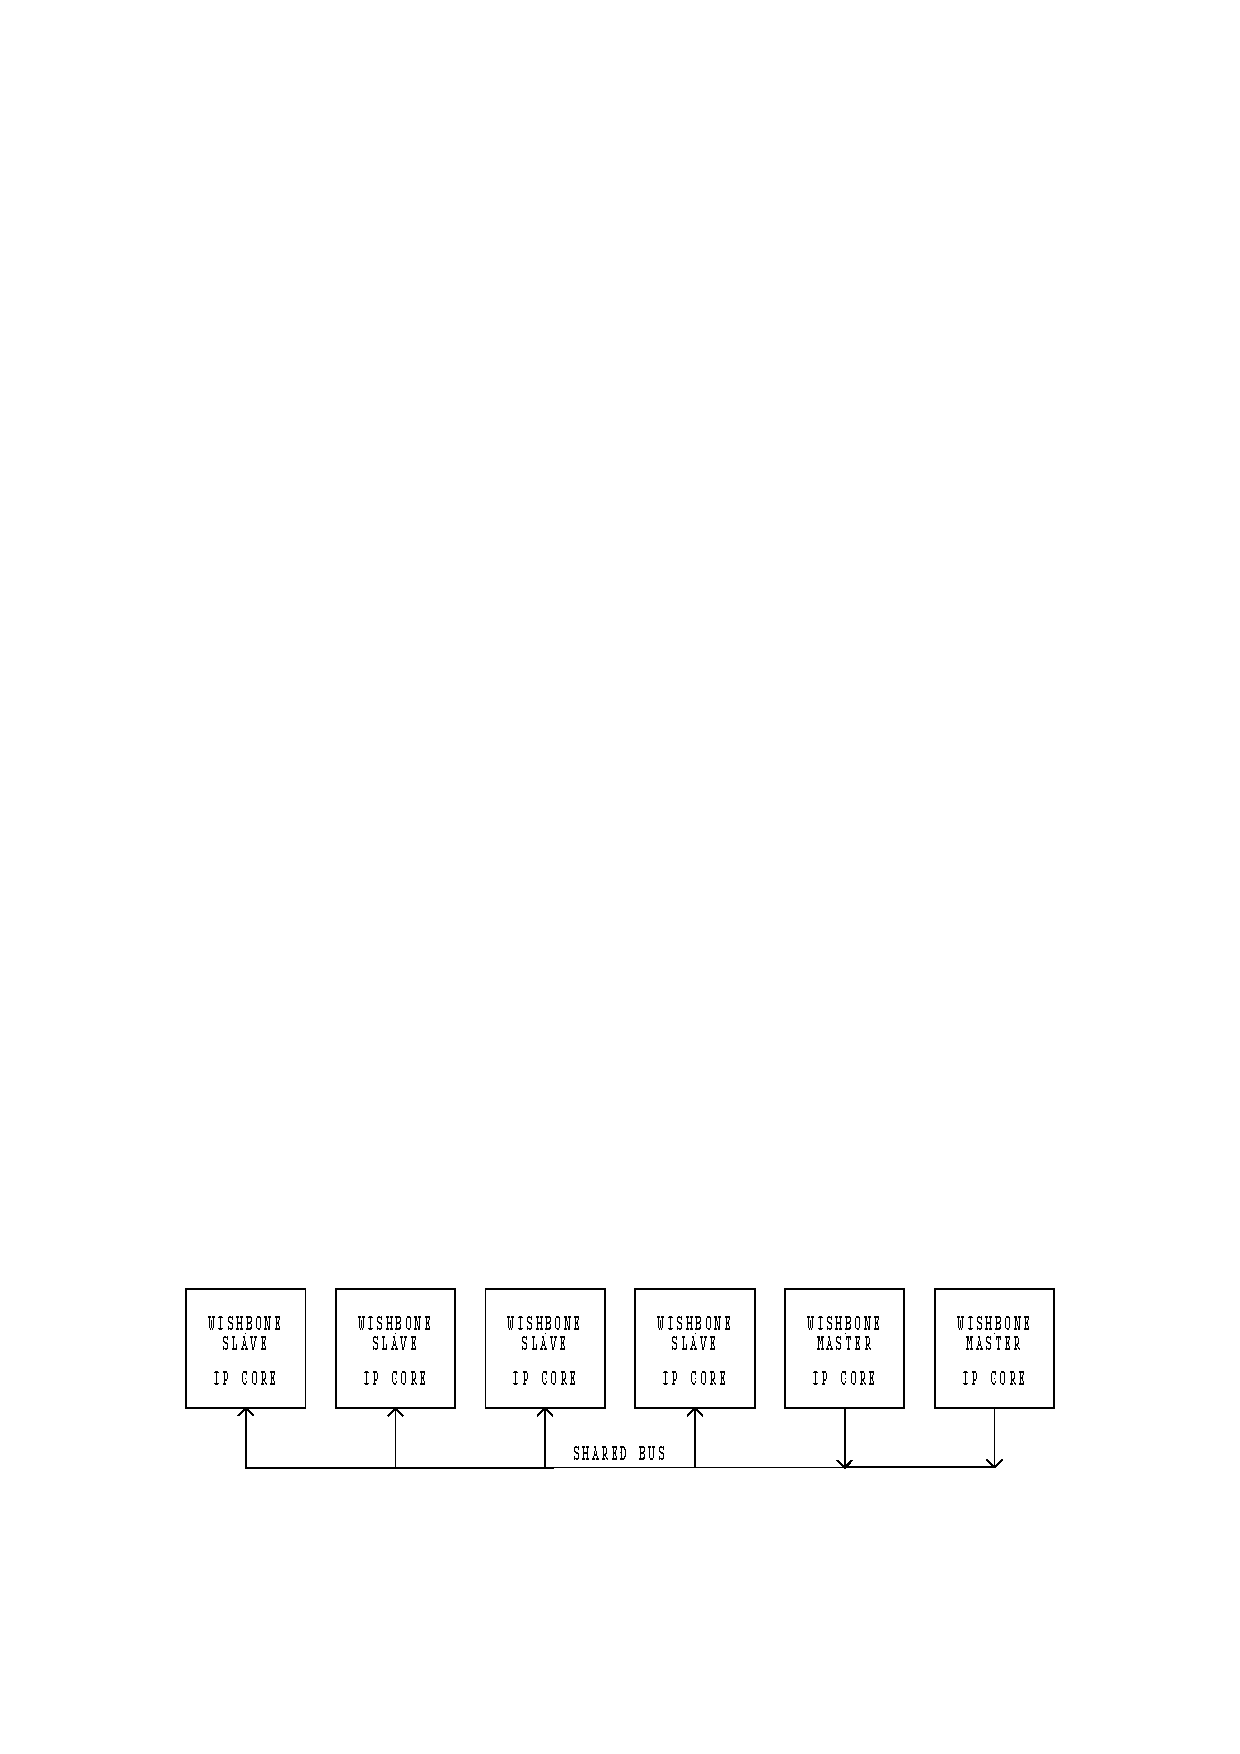
\includegraphics[width=0.9\linewidth]{images/shared_bus_interconnection}
	\caption{Shared bus \cites[21]{website:wishbone_b4_spec}}
	\label{fig:shared_bus_intercon}
\end{figure}

In \cref{fig:shared_bus_intercon} ist eine Shared-Bus-Topologie dargestellt. Hierbei initiiert ein Master einen Buszyklus zum Slave. Traditionelle Busse wie VMEbus und PCI Bus nutzen diese Topologie. Architekturbedingt kann hier nur ein Master zu einem Zeitpunkt den Bus nutzen. \cite[21]{website:wishbone_b4_spec}

\subsection{Wishbone}

Wishbone ist ein Open-Source-Hardware Computerbus, welcher die Kommunikation der Komponenten eines \gls{SoC} durch eine einheitliche Schnittstelle deutlich vereinfacht. Entwickelt wurde dieser von der Silicore Corporation, und später von OpenCores\footnote{\url{https://opencores.org}} veröffentlicht. Überwiegend wird Wishbone-Standard von quelloffenen Hardware-Projekten verwendet. 

Eine mögliche Portkonfiguration für Wishbone-Master bzw Slave ist in \cref{fig:standard_connection_for_timing_diagrams} dargestellt.

\begin{figure}[!htbp]
	\centering
	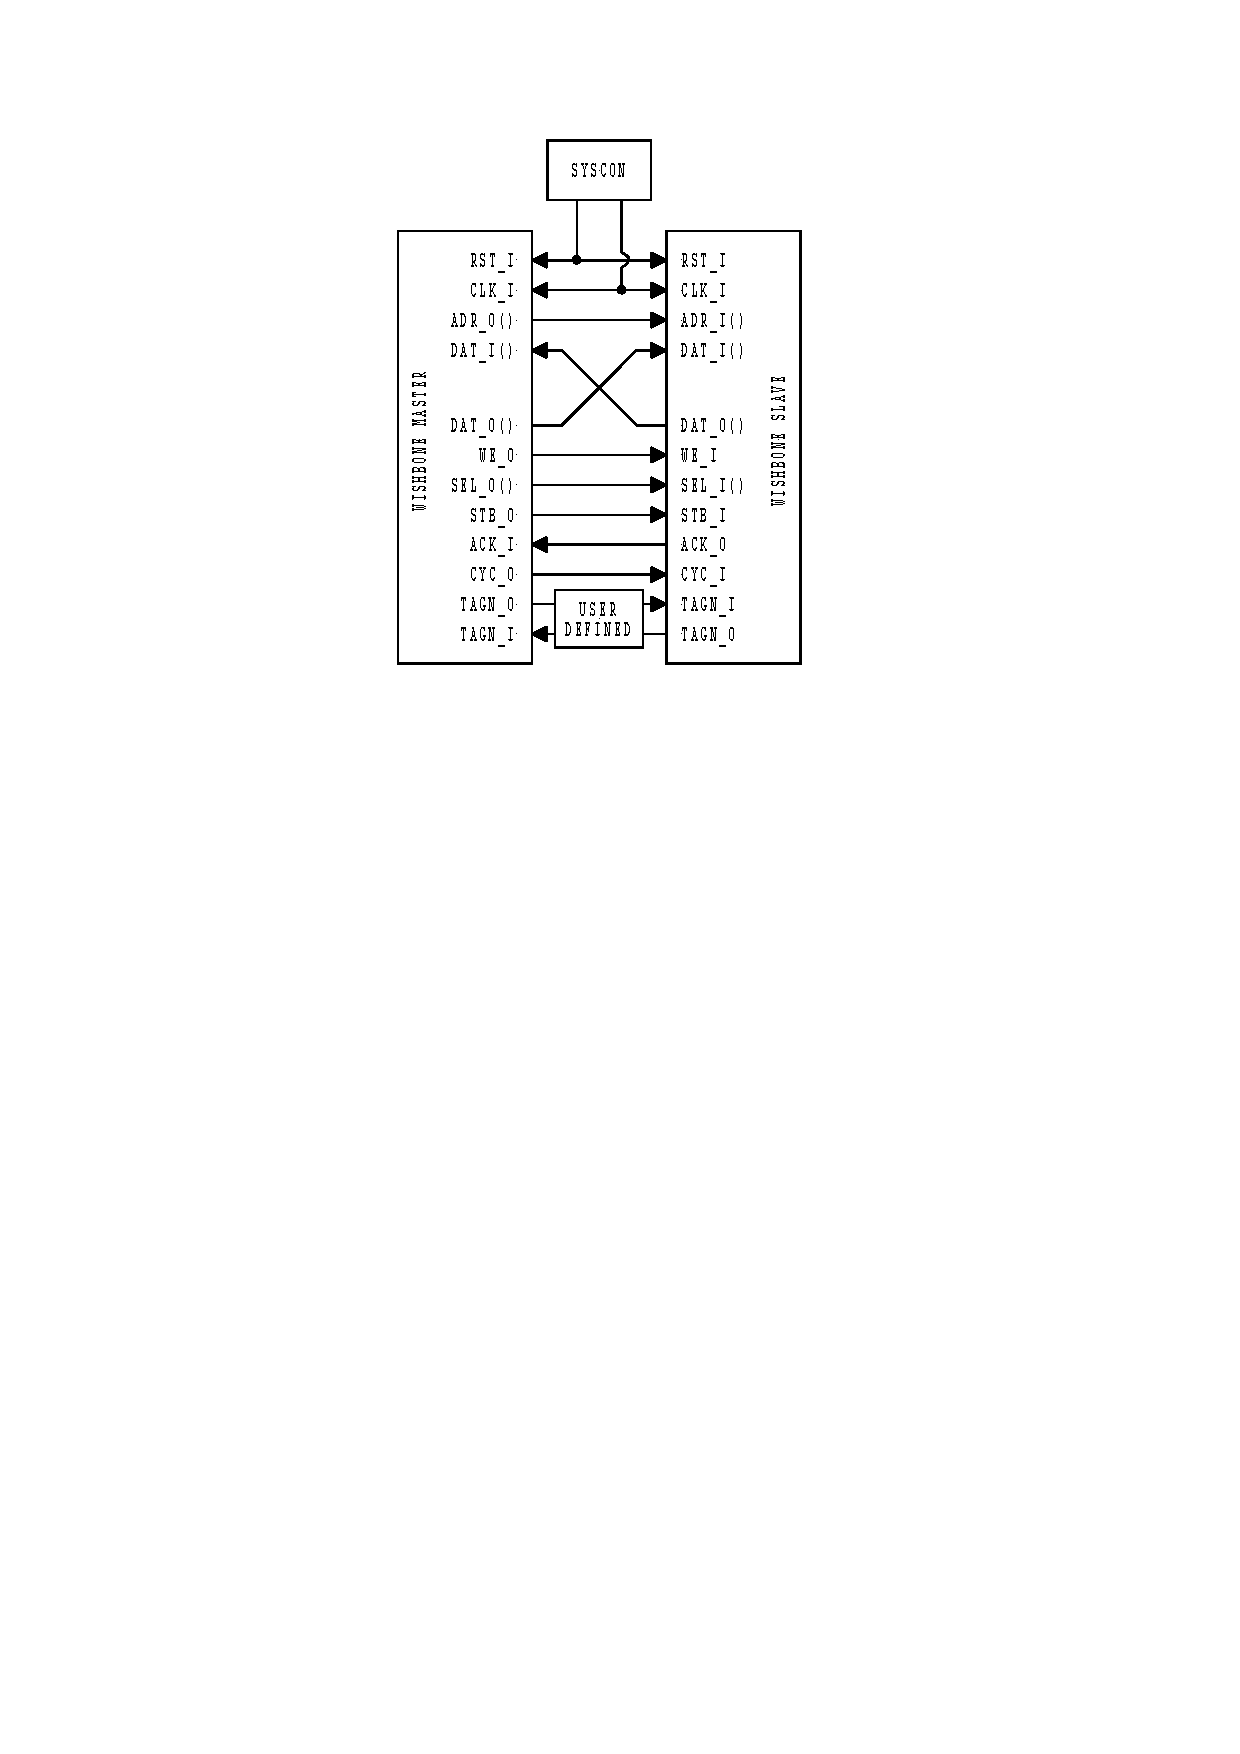
\includegraphics[width=0.5\linewidth]{images/standard_connection_for_timing_diagrams}
	\caption{Standard connection for timing diagrams \cite[14]{website:wishbone_b4_spec}}
	\label{fig:standard_connection_for_timing_diagrams}
\end{figure}

\subsection{Avalon}
\label{sec:theory_avalon}

Avalon ist eine proprietäre Bus-Architektur und wurde ursprünglich von Altera entwickelt, um On-Chip-Prozessoren und Peripherie zu einem \gls{SOPC} zu verknüpfen. \cite[{7-6}]{article:soc_buses} Nutzbar ist Avalon als eine Sammlung parametrisierbarer IP-Cores, die vom Platform Designer (früher als Qsys bzw. SOPC Builder bekannt) im Laufe der Systementwicklung automatisch generiert und parametrisert werden. 

Ein mögliches System mit Avalon ist auf \cref{fig:avalon_bus_based_system} abgebildet.

\begin{figure}[!htbp]
	\centering
	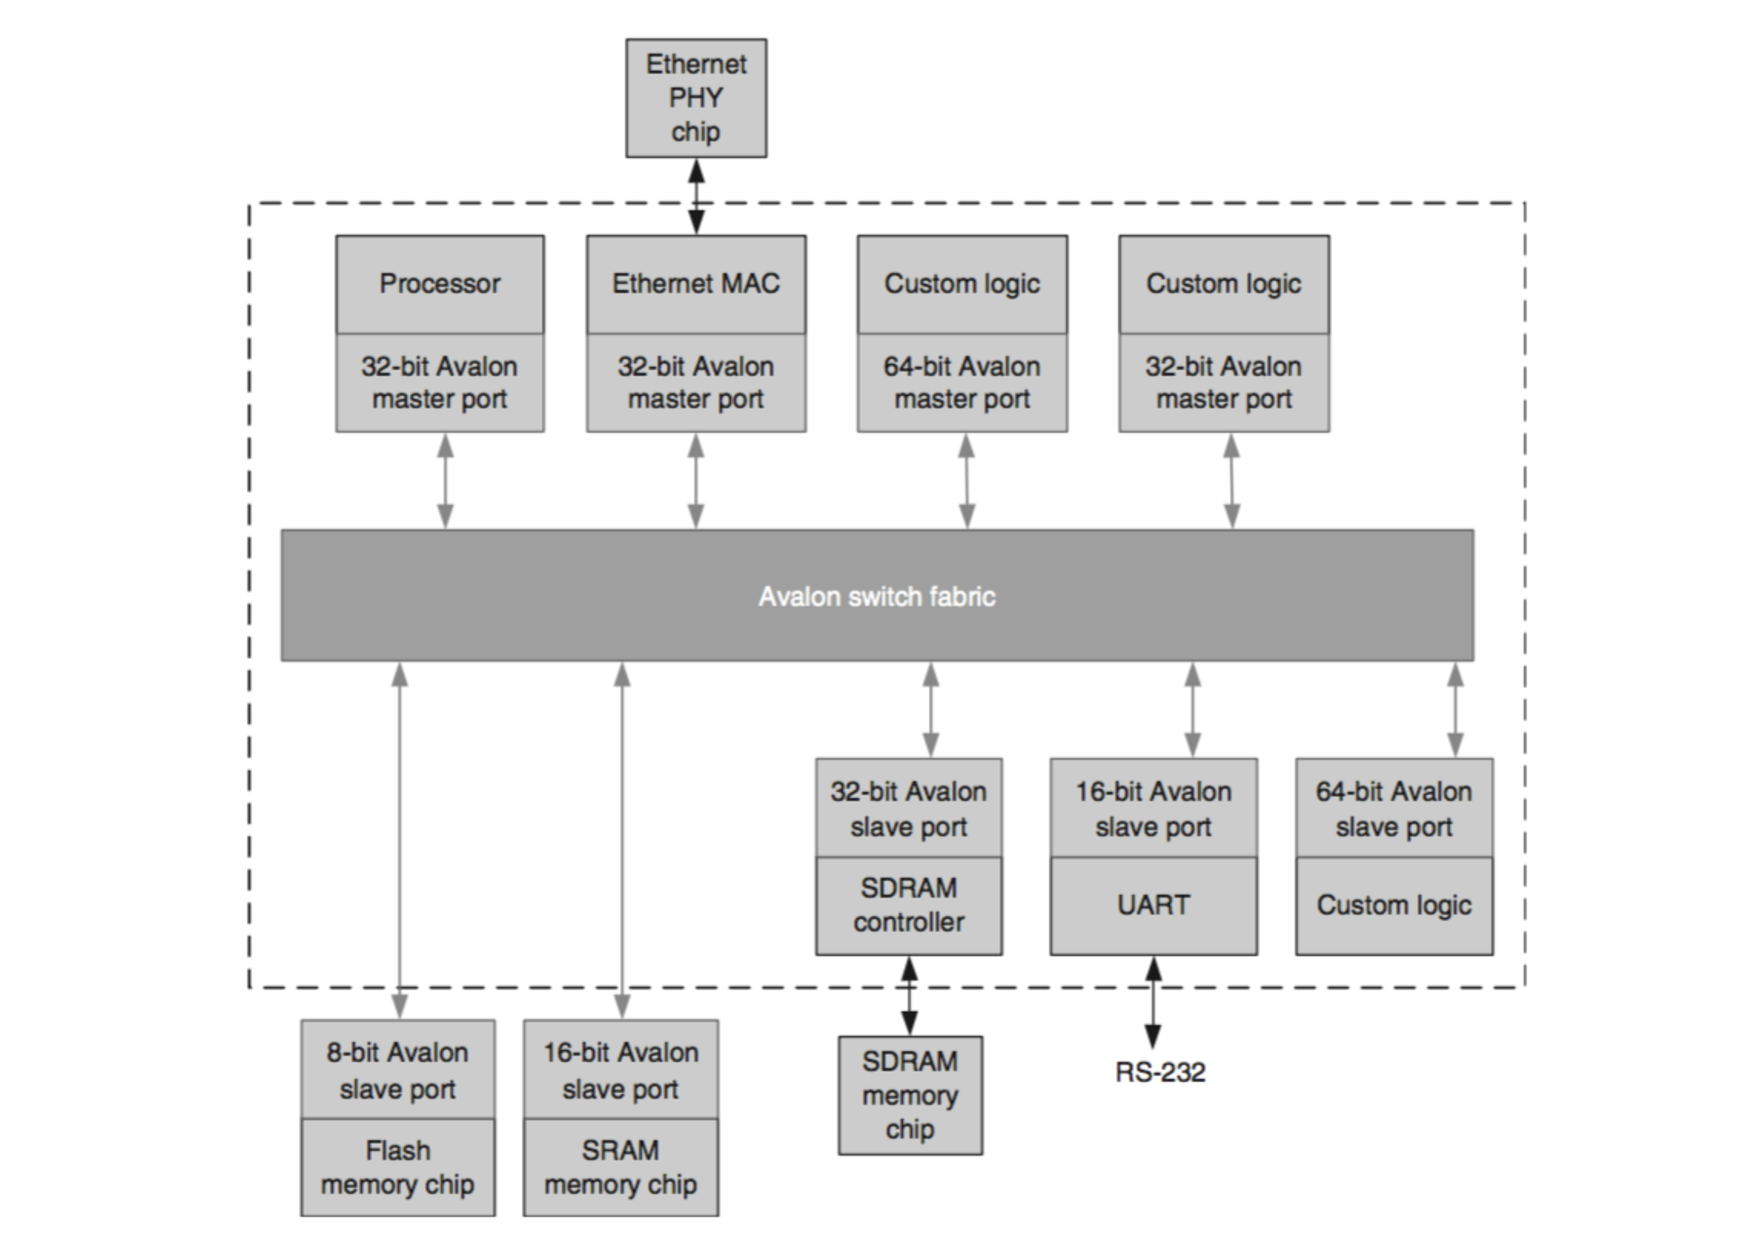
\includegraphics[width=0.7\linewidth]{images/avalon_bus_based_system}
	\caption{Avalon-Bus basiertes System \cite[{7-6}]{article:soc_buses}}
	\label{fig:avalon_bus_based_system}
\end{figure}

Die Avalon-Spezifikation sieht sieben Schnittstellentypen vor \cite[4]{manual:avalon_spec}: 
\begin{easylist}[itemize]
	& Avalon Streaming Interface (Avalon-ST) - unterstützt unidirektionalen Datenfluss (vgl. \cref{fig:data_flow_intercon})
	& Avalon Memory Mapped Interface (Avalon-MM) - unterstützt adressbasierte bidiriektionale Master-Slave Kommunikation 
	& Avalon Conduit Interface - fasst Signale, die nicht einem Avalon-Schnittstellentyp zuzuordnen sind, zusammen. Eine Verbindung im Platform Designer bzw. Export zur manuellen Verknüpfung ist möglich
	& Avalon Tri-State Conduit Interface (Avalon-TC) - unterstützt Verbindungen zu Off-Chip Komponenten. Mehrere Peripheriegeräte können Pins durch Signalmultiplexing teilen
	& Avalon Interrupt Interface - ermöglicht Komponenten Ereignisse an andere Komponenten zu vermitteln
	& Avalon Clock Interface - Schnittstelle für Taktein- bzw. Ausgang
	& Avalon Reset Interface - Schnittstelle für Reset-Logik	
\end{easylist}

Avalon nutzt separate Adress-, Daten-, und Steuerleitungen. \cite[7-6]{article:soc_buses}
In \cref{tab:avalonmm_signals} sind die für diese Arbeit wichtigsten Avalon-MM Signale aufgelistet.
\begin{table}[!htbp]
	\bigskip
	\centering
	\begin{tabular}{  l | l }
		\textbf{Signal} & \textbf{Beschreibung} \\
		\hline
		address & Adresse \\
		byteenable & Byte-Selektor \\		
		read & Signalisiert einen Lesezugriff \\ 
		write & Signalisiert einen Schreibzugriff \\ 
		readdata & Vom Slave übertragenes Datenwort \\
		writedata & An den Slave übertragenes Datenwort \\
		waitrequest & An den Master übermitteltes Wartesignal \\
		response & Optionaler Antwortcode \\
		\hline
	\end{tabular}
	
	\caption{Avalon-MM Signale \cite[14-16]{manual:avalon_spec}}
	\label{tab:avalonmm_signals}
\end{table}

\section{Plasma CPU}
\label{the:plasma}

Die Plasma \gls{CPU} ist ein kleiner, synthetisierbarer 32-bit \gls{RISC} Mikroprozessor. Derzeit führt es einen Webserver mit einem Interruptcontroller, \gls{UART}, \gls{SRAM} oder \gls{DDR SDRAM} Controller, und einem Ethernetcontroller aus. Die Plasma CPU führt bis auf unausgerichtete Lade und Speicheroperationen alle \gls{MIPS} \RN{1} User-Mode Instruktionen aus \cite{website:plasma_cpu}.

Der auf dem Plasma ausgeführte Webserver ist unter der angegebenen Adresse \textit{https://plasmacpu.no-ip.org:8080/} \cite{website:plasma_cpu}, geprüft am \DTMdate{2018-04-22}, nicht erreichbar.

In \cref{fig:plasma_cpu_block_diagram} ist das Block-Diagramm der Plasma-\gls{CPU} dargestellt.

\begin{figure}[!htbp]
	\centering
	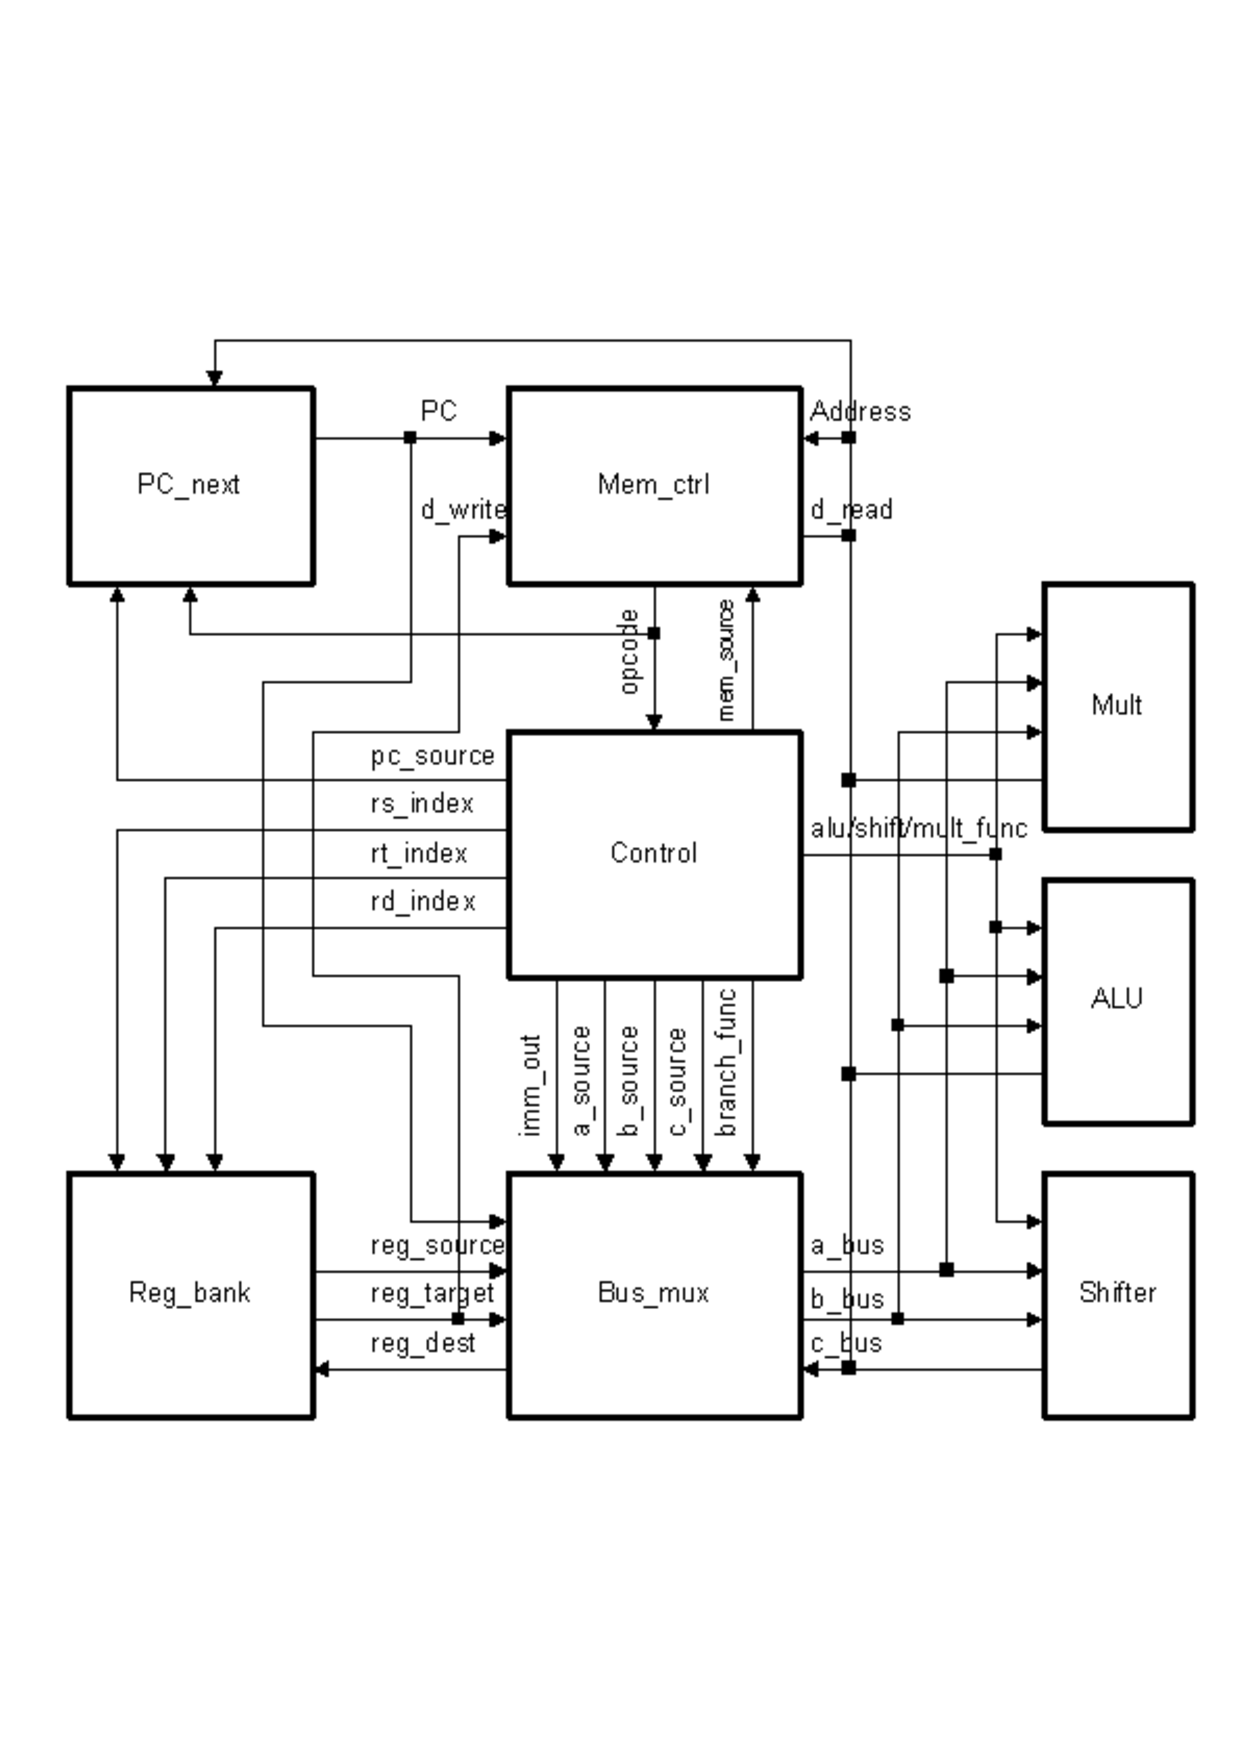
\includegraphics[width=0.6\linewidth]{images/plasma_block_diagram}
	\caption{Plasma-CPU Blockdiagramm \cite{website:plasma_cpu}}
	\label{fig:plasma_cpu_block_diagram}
\end{figure}



\section{Device Tree}

Der Device Tree ist eine baumartige Datenstruktur, mit der eine deklarative Beschreibung der auf einem System verfügbaren Hardware  möglich ist. Jeder Knoten hat Schlüssel/Wert-Paare, welche die Charakteristika des repräsentierten Geräts beschreiben. Die Baum-Struktur ist dadurch gegeben, dass jeder Knoten genau einen Elternknoten besitzt. Die einzige Ausnahme ist der Wurzelknoten, welcher keinem Elternknoten zugeordnet ist \cite[6]{manual:devicetree_specification}. 

Bevor die Device Tree-Spezifikation eingeführt wurde, beinhaltete der Linux-Kernel gerätespezifischen Code. Bereits geringfügige Änderungen, wie die Änderung einer Basisadresse, führten dazu, dass der ganze Kernel neu kompiliert werden musste \cite[1]{manual:intro_to_devicetrees}. 

Für eingebettete Systeme, welche im Gegensatz zu größeren Systemen wie Desktop-Computern nur selten über automatische Erkennungsmechanismen neuer Hardware verfügen, bedeutet es einen enormen Entwicklungs- und Wartungsaufwand. Dieser Aufwand übertrug sich auch auf die Kernel-Entwickler, die Unmengen an verschiedensten Systemkonfigurationen im Kernel verwalten mussten.  

%In \cref{lst:dts_gpio_expl} ist eine beispielhafte Definition für ein \gls{GPIO}-Device dargestellt. Diese wird schrittweise näher erklärt. 
%\begin{code}
%	\begin{minted}[breaklines, autogobble]{text}
%	gpio0: gpio@ff708000 {
%		#address-cells = <1>;
%		#size-cells = <0>;
%		compatible = "snps,dw-apb-gpio";
%		reg = <0xff708000 0x1000>;
%		clocks = <&l4_mp_clk>;
%		status = "disabled";
%		
%		porta: gpio-controller@0 {
%			compatible = "snps,dw-apb-gpio-port";
%			gpio-controller;
%			#gpio-cells = <2>;
%			snps,nr-gpios = <29>;
%			reg = <0>;
%			interrupt-controller;
%			#interrupt-cells = <2>;
%			interrupts = <0 164 4>;
%		};
%	};
%	\end{minted}
%	
%	\caption{Devicetree: Komponenten am Avalon-Bus}
%	\label{lst:dts_gpio_expl}
%\end{code}
%
%
%Der Ausdruck \texttt{gpio0} definiert das Label, wodurch die nachfolgende Gerätebeschreibung an anderen Stellen referenziert werden kann. Der Ausdruck \texttt{gpio} definiert den Gerätetypen und \texttt{ff708000} die Basisadresse:
%\begin{minted}[breaklines, autogobble]{text}
%	gpio0: gpio@ff708000
%\end{minted}
%
%Das Rautenzeichen (\#) gibt an, dass der Schlüssel einen \SI{32}{\bit} breiten vorzeichenlosen Ganzzahlwert annimmt.
%Mit \texttt{address-cells} und \texttt{size-cells} wird die Adressierungsart der Kinderknoten spezifiziert. In diesem Beispiel werden \SI{32}{\bit} (eine Zelle) für die Adresskodierung und \SI{0}{\bit} (0 Zellen) für den Adressbereich genutzt:
%\begin{minted}[breaklines, autogobble]{text}
%#address-cells = <1>;
%#size-cells = <0>;
%\end{minted}
%
%Der Schlüssel \texttt{compatible} gibt den kompatiblen Treiber an. Wenn dieser vorhanden ist, so wird er vom Kernel geladen und an diese Gerätebeschreibung gebunden:
%\begin{minted}[breaklines, autogobble]{text}
%compatible = "snps,dw-apb-gpio";
%\end{minted}
%
%Mit dem \texttt{reg}-Schlüssel wird nochmals die Basisadresse angegeben. Hinzu kommt der Adressbereich \texttt{0x1000}:
%\begin{minted}[breaklines, autogobble]{text}
%reg = <0xff708000 0x1000>;
%\end{minted}
%
%Der \texttt{clocks}-Schlüssel gibt die Taktgeber an. Hierbei wird auch der Einsatz einer Referenz auf ein definiertes Label mit \&label\_name deutlich:
%\begin{minted}[breaklines, autogobble]{text}
%clocks = <&l4_mp_clk>;
%\end{minted}
%
%Ein Gerät kann sich in drei allgemeinen Zuständen befinden: \enquote{okay} (Betriebsbereit), \enquote{disabled} (Deaktiviert bzw. nicht angeschlossen) und \enquote{fail} (Fehlerzustand). Dies wird mit dem \texttt{status}-Schlüssel angegeben:
%\begin{minted}[breaklines, autogobble]{text}
%status = "disabled";
%\end{minted}
%
%Ein untergeordnetes Gerät mit dem Label \texttt{porta} wird definiert:
%\begin{minted}[breaklines, autogobble]{text}
%porta: gpio-controller@0
%\end{minted}
%
%Es ist möglich, treiberspezifische Schlüssel zu setzen, welche für die geladenen Treiber aus der \texttt{compatible}-Liste gelten:
%\begin{minted}[breaklines, autogobble]{text}
%snps,nr-gpios = <29>;
%\end{minted}
%
%Der \texttt{interrupt}-Schlüssel definiert die von diesem Gerät emittierten Interrupts:
%\begin{minted}[breaklines, autogobble]{text}
%interrupts = <0 164 4>;
%\end{minted}

\section{Lebenszyklus des Cyclone V SoCFPGA}

Am Startvorgang eines komplexen Rechnersystems sind etappenweise mehrere Softwaresysteme beteiligt. So kann die Firmware die initiale Hardwarekonfiguration vornehmen, um dann die Kontrolle an eine weitere Software wie z.B einen Bootloader oder ein Betriebssystem zu übergeben \cite[3]{manual:devicetree_specification}. Das Standard-Szenario für Altera SoCFPGA-Systeme ist in \cref{fig:bootflow} abgebildet.

\begin{figure}[!htbp]
	\centering
	\begin{tikzpicture}[node distance=2cm, scale=0.6, every node/.style={scale=0.6}]
	\node (reset) [startstop] {Reset};
	\node (bootrom) [process, below of=reset, align = center] {Boot ROM};
	\node (preloader) [process, below of=bootrom, align = center] {Preloader};
	\node (uboot) [process, below of=preloader, align = center] {Bootloader (U-Boot)};
	\node (linux) [process, below of=uboot, align = center] {OS (Linux)};
	\node (app) [startstop, below of=linux, align = center] {Benutzeranwendung};
	
	\draw [->] (reset) -- (bootrom);
	\draw [->] (bootrom) -- (preloader);
	\draw [->] (preloader) -- (uboot);	
	\draw [->] (uboot) -- (linux);
	\draw [->] (linux) -- (app);
	
	\end{tikzpicture}
	\caption{Bootvorgang \cite[95]{manual:ws2_kernel_intro}}
	\label{fig:bootflow}
\end{figure}

Der erste Bootloader befindet sich im BootROM und ist fest vom Hersteller Altera einprogrammiert. Seine Aufgabe besteht darin, den \gls{MBR}-Eintrag der Speicherkarte auszulesen, die Altera-spezifische Partition mit der Kennung \texttt{0xA2} zu identifizieren und den Preloader vom Anfang der Partition zu verifizieren und auszuführen \cite[98]{manual:ws2_kernel_intro}. 

Die Aufgabe des Preloaders besteht darin, sämtliche Taktgeneratoren, \glspl{PLL}, \glspl{RAM}, \glspl{IO} und Pin-Multiplexer zu initialisieren. Im Anschluss wird vom Preloader von der Partition mit der Kennung \texttt{0xA2} der nächste Bootloader, wie z.B. \enquote{Das U-Boot}, verifiziert, geladen und gestartet. 

Werden die \gls{HPS}-Peripherieeinstellungen im Platform Designer verändert, so muss der Preloader neu generiert, kompiliert und auf das Startmedium übertragen werden \cite[96]{manual:ws2_kernel_intro}.

\alertwarning{Eine häufige Fehlerquelle ist ein veralteter Preloader. Dieser muss bei jeder Änderung der \gls{HPS}-Konfiguration im Platform Designer aktualisiert werden! \cite[96]{manual:ws2_kernel_intro}}

Für eingebettete Systeme eignet sich der Bootloader \enquote{Das U-Boot}. Dieser Bootloader ist quelloffen, portabel, bietet Treiber für ein breites Spektrum an Peripheriegeräten und richtet eine Umgebung mit einer Kommandozeile ein. Außerdem lädt er den Device Tree und ist in der Lage, diesen zur Laufzeit mit aktuellen Daten zu modifizieren. Sobald die Umgebung eingerichtet ist, lädt dieser Bootloader den Linux-Kernel vom Dateisystem, Netzwerk oder serieller Schnittstelle und übergibt sämtliche Bootargumente an den Kernel \cite[105-106]{manual:ws2_kernel_intro}.
	\chapter{Systemarchitektur}
\label{cha:architecture}

Dieses Kapitel beschreibt die vorhandene Architektur, schlägt neue vor und dient dem besseren Verständnis über die Umsetzung in \cref{cha:implementation}.

Im \cref{sec:arch_plasma} wird die Architektur des Ausgangssystems in der Version 2.1 beschrieben.

Im \cref{sec:arch_plasma_soc_zedboard} wird eine neue Architektur, die den Wishbone-\gls{Interconnect} nutzt, neue Komponenten aufweist und speziell auf das Zedboard zugeschnitten ist, vorgestellt. 

Im \cref{sec:arch_plasma_soc_de1_soc} werden zwei neue Architekturen vorgeschlagen. Die erste stellt einer Portierung auf das DE1-SoC Board dar, in der zweiten wird die erste Architektur erneut aufgegriffen und erweitert. 

\tikzstyle{block} = [draw, fill=white, rectangle, minimum height=3em, minimum width=6em]

\tikzset{
	block crossed out/.style={
		block,
		append after command={
			node [
				fit=(\tikzlastnode),
				draw=red,
				thick,
				inner sep=-\pgflinewidth,
				cross out
			] {}
		}
	}
}

\tikzstyle{sum} = [draw, fill=white, circle, node distance=1cm]
\tikzstyle{pinstyle} = [pin edge={to-,thin,black}]
\tikzstyle{container} = [draw, rectangle, dashed, inner sep=2em]

\section{Plasma}
\label{sec:arch_plasma}

Auf \cref{fig:sysarch_plasma} ist die Architektur des Plasma-Systems im Ausgangszusatand (Version 2.1) abgebildet. Diese beinhaltet nur einen rudimentären Interrupt-Controller, zwei \glspl{GPIO}, einen Counter sowie einen \gls{UART} Controller. Außerdem ist der interne \gls{RAM} als \gls{FPGA}-interner Block-\gls{RAM} implementiert und der externe \gls{RAM} ungenutzt. Die Verknüpfung zwischen der Plasma-CPU und den Komponenten erfolgt über einen sehr einfachen Multiplexer mit Adressdekoder, dessen Erweiterung sich allerdings als äußerst umständlich erweist. 

\begin{figure}[!htbp]
	\centering	
	\begin{tikzpicture}[auto]
	\node [block] (plasma) {Plasma CPU};
	\node [block, below = of plasma.south west, anchor=north west, minimum width = \linewidth] (intercon) {MUX};
	
	\node [block, below = of intercon.south west, anchor=north west, xshift=1cm] (irq) {IRQ};
	\node [block, right = of irq] (iram) {Int. RAM};
	\node [block, below = of iram] (eram) {Ext. RAM};
	
	\node [block, right = of iram] (gpios) {GPIO\textsubscript{0..1}};
	\node [block, below = of gpios] (counters) {CNT\textsubscript{0}};	
	
	\node [block, right = of gpios] (uartc) {UART};
	
	\draw[->]             (plasma.south) -- (plasma.south |- intercon.north);
	
	\draw[<-]             (irq.west) -- ++(-5mm, 0) -- (\currentcoordinate |- intercon.south); 
	
	\draw[<-]             (iram.west) -- ++(-5mm, 0) -- (\currentcoordinate |- intercon.south);
	\draw[<-]             (eram.west) -- ++(-5mm, 0) -- (\currentcoordinate |- intercon.south);
	
	\draw[<-]             (gpios.west) -- ++(-5mm, 0) -- (\currentcoordinate |- intercon.south);
	\draw[<-]             (counters.west) -- ++(-5mm, 0) -- (\currentcoordinate |- intercon.south);
	
	\draw[<-]             (uartc.west) -- ++(-5mm, 0) -- (\currentcoordinate |- intercon.south);
	\end{tikzpicture}
	
	\caption{Blockdiagramm des Plasma im Ausgangszustand}
	\label{fig:sysarch_plasma}
\end{figure}

\section{Plasma-SoC auf dem ZedBoard}
\label{sec:arch_plasma_soc_zedboard}

Die erste Entwicklungsiteration erfolgt für das Digilent ZedBoard. Es werden ein Wishbone-\gls{Interconnect} und die dazugehörigen Wrapper bzw. Adapter entwickelt. 
Außerdem werden neue Komponenten wie z.B. Zähler, ein Controller für das Display mit der Modellnummer UG-2832HSWEG04 sowie ein \gls{SPI}-Controller eingeführt. Einen Überblick über die neue Systemarchitektur verschafft \cref{fig:sysarch_plasmasoc_zedboard}.
\begin{figure}[!htbp]
	\centering	
	\begin{tikzpicture}[auto]
	\node [block] (plasma) {Plasma CPU};
	\node [block, right = of plasma] (arbiter) {Arbiter};
	\node [block, below = of plasma.south west, anchor=north west, minimum width = \linewidth] (intercon) {Wishbone Intercon};
	
	\node [block, below = of intercon.south west, anchor=north west, xshift=1cm] (irc) {IRC};
	\node [block, right = of irc] (iram) {Int. RAM};
	\node [block, below = of iram] (eram) {Ext. RAM};
	
	\node [block, right = of iram] (gpios) {GPIO\textsubscript{0..3}};
	\node [block, below = of gpios] (counters) {CNT\textsubscript{0..3}};
	\node [block, below = of counters] (timers) {TIM\textsubscript{0..3}};
	
	\node [block, right = of gpios] (uartc) {UART};
	\node [block, below = of uartc] (oledc) {Display};
	\node [block, below = of oledc] (spic) {SPI};
	
	\draw[->]             (plasma.east) -- (arbiter.west);
	
	\draw[->]             (plasma.south) -- (plasma.south |- intercon.north);
	\draw[->]             (arbiter.south) -- (arbiter.south |- intercon.north);
	
	\draw[<-]             (irc.west) -- ++(-5mm, 0) -- (\currentcoordinate |- intercon.south); 
	
	\draw[<-]             (iram.west) -- ++(-5mm, 0) -- (\currentcoordinate |- intercon.south);
	\draw[<-]             (eram.west) -- ++(-5mm, 0) -- (\currentcoordinate |- intercon.south);
	
	\draw[<-]             (gpios.west) -- ++(-5mm, 0) -- (\currentcoordinate |- intercon.south);
	\draw[<-]             (counters.west) -- ++(-5mm, 0) -- (\currentcoordinate |- intercon.south);
	\draw[<-]             (timers.west) -- ++(-5mm, 0) -- (\currentcoordinate |- intercon.south);
	
	\draw[<-]             (oledc.west) -- ++(-5mm, 0) -- (\currentcoordinate |- intercon.south);
	\draw[<-]             (uartc.west) -- ++(-5mm, 0) -- (\currentcoordinate |- intercon.south);
	\draw[<-]             (spic.west) -- ++(-5mm, 0) -- (\currentcoordinate |- intercon.south);
	\end{tikzpicture}
	
	\caption{Blockdiagramm des Plasma-SoC auf dem ZedBoard}
	\label{fig:sysarch_plasmasoc_zedboard}
\end{figure}

\section{Plasma auf dem DE1-SoC-Board}
\label{sec:arch_plasma_soc_de1_soc}

In der zweiten Iteration wird das vorhandene Plasma-SoC auf das neue Terasic DE1-SoC-Board portiert. Die dabei verfolgte Architektur ist auf \cref{fig:sysarch_plasmasoc_de1_soc} abgebildet.
Da das Terasic DE1-SoC-Board nicht über ein Display verfügt, wird dieser aus dem Wishbone-Bus und der Adresszuordnung entfernt. Ebenso wird auf die externe \gls{RAM}-Schnittstelle verzichtet. 

\begin{figure}[!htbp]
	\centering	
	\begin{tikzpicture}[auto]
	
	\node [block] (plasma) {Plasma CPU};
	\node [block, right = of plasma] (arbiter) {Arbiter};
	\node [block, below = of plasma.south west, anchor=north west, minimum width = \linewidth] (intercon) {Wishbone Intercon};
	
	\node [block, below = of intercon.south west, anchor=north west, xshift=1cm] (irc) {IRC};
	\node [block, right = of irc] (iram) {Int. RAM};
	\node [block crossed out, below = of iram] (eram) {Ext. RAM};
	
	\node [block, right = of iram] (gpios) {GPIO\textsubscript{0..3}};
	\node [block, below = of gpios] (counters) {CNT\textsubscript{0..3}};
	\node [block, below = of counters] (timers) {TIM\textsubscript{0..3}};
	
	
	\node [block, right = of gpios] (uartc) {UART};
	\node [block crossed out, below = of uartc] (oledc) {Display};
	\node [block, below = of oledc] (spic) {SPI};
	
	\draw[->]             (plasma.east) -- (arbiter.west);
	
	\draw[->]             (plasma.south) -- (plasma.south |- intercon.north);
	\draw[->]             (arbiter.south) -- (arbiter.south |- intercon.north);
	
	\draw[<-]             (irc.west) -- ++(-5mm, 0) -- (\currentcoordinate |- intercon.south); 
	
	\draw[<-]             (iram.west) -- ++(-5mm, 0) -- (\currentcoordinate |- intercon.south);
	\draw[<-]             (eram.west) -- ++(-5mm, 0) -- (\currentcoordinate |- intercon.south);
	
	\draw[<-]             (gpios.west) -- ++(-5mm, 0) -- (\currentcoordinate |- intercon.south);
	\draw[<-]             (counters.west) -- ++(-5mm, 0) -- (\currentcoordinate |- intercon.south);
	\draw[<-]             (timers.west) -- ++(-5mm, 0) -- (\currentcoordinate |- intercon.south);
	
	\draw[<-]             (oledc.west) -- ++(-5mm, 0) -- (\currentcoordinate |- intercon.south);
	\draw[<-]             (uartc.west) -- ++(-5mm, 0) -- (\currentcoordinate |- intercon.south);
	\draw[<-]             (spic.west) -- ++(-5mm, 0) -- (\currentcoordinate |- intercon.south);
	
	\end{tikzpicture}
	\caption{Blockdiagramm des Plasma-SoC auf dem DE1-SoC}
	\label{fig:sysarch_plasmasoc_de1_soc}
\end{figure}

Die dritte Iteration sieht eine Erweiterung des auf das Terasic DE1-SoC-Board portierten Plasma-SoC vor. In diesem Schritt werden jeweils eine Avalon-Wishbone und eine Wishbone-Avalon Bridge als Master bzw. Slave zum Wishbone-Bus hinzugefügt, wie auf \cref{fig:sysarch_plasmasoc_de1_soc_qsys} dargestellt. Diese Neuerung und die Erstellung eines IP-Core ermöglicht eine Integration in das das im Platform Designer entworfene QSYS-System. 

\begin{figure}[!htbp]
	\centering	
	\begin{tikzpicture}[auto]
	
	\node [block] (hps) {HPS (ARM CPU)};
	\node [block, right = of hps] (sysid) {SysID};
		
	\node [block, below = 1.5cm of hps.south west, anchor=north west, minimum width = \linewidth] (avalons) {Avalon Bridge (Wishbone Master)};
	
	\node [block, below = of avalons.south west, anchor=north west] (plasma) {Plasma CPU};
	\node [block, right = of plasma] (arbiter) {Arbiter};
	\node [block, below = of plasma.south west, anchor=north west, minimum width = \linewidth] (intercon) {Wishbone Intercon};
	
	\node [block, below = of intercon.south west, anchor=north west, xshift=1cm] (irc) {IRC};
	\node [block, right = of irc] (iram) {Int. RAM};
	
	\node [block, right = of iram] (gpios) {GPIO\textsubscript{0..3}};
	\node [block, below = of gpios] (counters) {CNT\textsubscript{0..3}};
	\node [block, below = of counters] (timers) {TIM\textsubscript{0..3}};
	
	\node [block, right = of gpios] (uartc) {UART};
	\node [block, below = of uartc] (spic) {SPI};
	
	\node [block, below = 7.5cm of intercon.south east, anchor=north east, minimum width = \linewidth] (avalonm) {Avalon Bridge (Wishbone Slave)};
	
	\node [block, below = 1.5cm of avalonm.south west, anchor=north west, xshift=1cm] (eram) {Ext. RAM};
	\node [block, right = of eram] (hex) {7 segment display};
	\node [block, right = of hex] (switches) {Schalter};
	\node [block, right = of switches] (buttons) {Taster};
	
	
	\node[container, fit=(plasma) (intercon) (avalons) (avalonm)] (plasmasoc) {};
	\node at (plasmasoc.north west) [above right] {Plasma SoC};
	
	\draw[->]             (plasma.east) -- (arbiter.west);
	\draw[<-]             (arbiter.east) -- ++(5mm, 0) -- (\currentcoordinate |- avalons.south); 
	
	\draw[->]             (hps.south) -- (hps.south |- avalons.north);
	\draw[->]             (hps.east) -- (sysid.west);
	
	\draw[->]             (avalons.355) -- (intercon.5);
	
	\draw[->]             (plasma.south) -- (plasma.south |- intercon.north);
	\draw[->]             (arbiter.south) -- (arbiter.south |- intercon.north);
	
	\draw[<-]             (irc.west) -- ++(-5mm, 0) -- (\currentcoordinate |- intercon.south); 
	
	\draw[<-]             (iram.west) -- ++(-5mm, 0) -- (\currentcoordinate |- intercon.south);
	
	\draw[<-]             (gpios.west) -- ++(-5mm, 0) -- (\currentcoordinate |- intercon.south);
	\draw[<-]             (counters.west) -- ++(-5mm, 0) -- (\currentcoordinate |- intercon.south);
	\draw[<-]             (timers.west) -- ++(-5mm, 0) -- (\currentcoordinate |- intercon.south);
	
	\draw[<-]             (uartc.west) -- ++(-5mm, 0) -- (\currentcoordinate |- intercon.south);
	\draw[<-]             (spic.west) -- ++(-5mm, 0) -- (\currentcoordinate |- intercon.south);
	
	\draw[->]             (intercon.355) -- (avalonm.5);	
	
	\draw[<-]             (eram.west) -- ++(-5mm, 0) -- (\currentcoordinate |- avalonm.south); 
	\draw[<-]             (hex.west) -- ++(-5mm, 0) -- (\currentcoordinate |- avalonm.south); 
	\draw[<-]             (switches.west) -- ++(-5mm, 0) -- (\currentcoordinate |- avalonm.south); 
	\draw[<-]             (buttons.west) -- ++(-5mm, 0) -- (\currentcoordinate |- avalonm.south); 
	
	\end{tikzpicture}
	\caption{Blockdiagramm des Plasma-SoC auf dem DE1-SoC mit Verbindung zu weiteren IP-Cores und ARM Prozessor über den Avalon-Bus}
	\label{fig:sysarch_plasmasoc_de1_soc_qsys}
\end{figure}
	\chapter{Umsetzung}
\label{cha:implementation}

In diesem Kapitel wird auf die Umsetzungsdetails der Hardware- und Softwareentwicklung, sowie der Systemeinrichtung eingegangen. 

Im \cref{sec:impl_wishbone} werden wesentliche Etappen der Entwicklung des Wisbone-\gls{Interconnect}, neuer Module und Wrapper für bereits vorhandene Komponenten geschildert, um nachvolgende Erweiterungen besser nachvollziehen zu können.

Die Entwicklung der Firmware für das Plasma-\gls{SoC} wird in \cref{sec:plasma_fw} umrissen.

Auf die Portierung des im \cref{sec:impl_wishbone} geschilderten \gls{SoC} auf das in dieser Bachelorarbeit verwendete DE1-SoC Board wird in \cref{sec:impl_port_hw_to_de1_soc} eingegangen. 

Im \cref{sec:impl_extend_hw_for_de1_soc} wird das System aus \cref{sec:impl_port_hw_to_de1_soc} um zusätzliche Hardware-Komponenten erweitert, sodass der externe, \SI{64}{\mega\byte} umfassende, \gls{RAM}  und auch die \gls{ARM}-\gls{CPU} verwendet werden können. 

Im \cref{sec:impl_extend_tools_for_de1_soc} wird die Erweiterung der Hilfssoftware geschildert.

Die Portierung der Plasma-Firmware und der Plasma-Beispielanwendung auf das DE1-SoC wird im \cref{sec:impl_port_plasma_sw_to_de1_soc} geschildert.

Der \cref{sec:impl_setup_linuxfor_de1_soc} beschreibt die Einrichtung eines Linux-Betriebssystems auf dem DE1-SoC Board und der dafür notwendigen Schritte. 

Im \cref{sec:impl_develop_linux_sw_for_de1_soc} wird die Entwicklung der Linux Anwendungen, welche mit auf dem \gls{HPS} ausgeführt werden und Zugriff auf das Plasma-\gls{SoC} haben, beschrieben.

Im \cref{sec:impl_develop_linux_drivers_for_de1_soc} wird die Entwicklung der Linux Treiber, welche einen alternativen Zugriff auf das Plasma-Soc erlauben, beschrieben.
\section{Entwicklung des Wishbone-basierten Systems}
\label{sec:impl_wishbone}

Im Ausgangssystem stehen alle Komponenten durch manuelle Adressdekodierung und Datenmultiplex dem Plasma zur Verfügung. Jegliche Erweiterung erforderte mehrere Eingriffe und Komponenten mit mehreren Kontroll- und Datenregistern waren nur sehr schwer einzubinden. 

Es wird ein Shared-Bus (vgl. \cref{fig:shared_bus_intercon}) gemäß der Wishbone-Spezifikation \cites[21]{website:wishbone_b4_spec} entwickelt. Als Entwicklungsgrundlage dient das \enquote{boschmitt/wishbone}\cite{website:boschmitt_wishbone} Projekt. 

Sollte eine Adresse außerhalb des gültigen Bereiches angesprochen werden, so signalisiert der Bus einen Busfehler. Ein Fehler wird ebenfalls signalisiert, wenn eine korrekt ausgewählte Komponente innerhalb ihrer eigenen Adressdekodierung eine Zugriffsverletzung feststellt. Um einen Busfehler an den Kernel weiterzugeben, wird der Interrupt 31 verwendet (vgl. \cref{tab:interrupts}).

Die Adressbereiche, welche bei der partiellen Adressdekodierung verwendet werden, sind in \cref{tab:wb_plasma_zedboard_address_map} aufgelistet.

\begin{table}[!htbp]
	\bigskip
	\centering
	\begin{tabular}{| l | r | r |}
		\hline	
		\textbf{Gerät} & \textbf{Startadresse} & \textbf{Adressbereich} \\
		\hline		
		Interner \gls{RAM} & \texttt{0x00000000} & \texttt{0x0FFFFFFF} \\
		Externer \gls{RAM} & \texttt{0x10000000} & \texttt{0x001FFFFF} \\
		\hline		
		IRC\textsubscript{0} & \texttt{0x20000000} & \texttt{0x1F} \\
		\hline		
		UART\textsubscript{0}& \texttt{0x20000100} & \texttt{0x0F} \\
		\hline
		\multirow{4}{*}{Timer\textsubscript{0:3}} & \texttt{0x20000200} & \texttt{0x0F} \\
		& \texttt{0x20000210} & \texttt{0x0F} \\
		& \texttt{0x20000220} & \texttt{0x0F} \\
		& \texttt{0x20000230} & \texttt{0x0F} \\
		\hline
		\multirow{4}{*}{Zähler\textsubscript{0:3}} & \texttt{0x20000300} & \texttt{0x0F} \\
		& \texttt{0x20000310} & \texttt{0x0F} \\
		& \texttt{0x20000320} & \texttt{0x0F} \\
		& \texttt{0x20000330} & \texttt{0x0F} \\
		\hline
		\multirow{4}{*}{GPIO\textsubscript{0:3}}  & \texttt{0x20000400} & \texttt{0x0F} \\
		& \texttt{0x20000410} & \texttt{0x0F} \\
		& \texttt{0x20000420} & \texttt{0x0F} \\
		& \texttt{0x20000430} & \texttt{0x0F} \\
		\hline
		SPI\textsubscript{0} & \texttt{0x20000500} & \texttt{0x0F} \\
		\hline
		Display & \texttt{0x40000000} & \texttt{0x7F} \\
		\hline
	\end{tabular}
	
	\caption{Adresszuordnung}
	\label{tab:wb_plasma_zedboard_address_map}
\end{table}

Um destruktive Änderungen an bereits vorhandenen Komponenten, wie der Plasma-CPU, \gls{RAM}, \gls{UART}, etc. zu vermeiden, werden Wishbone-Wrapper als zusätzliche Entitäten entwickelt. Dieses Entwurfsmuster wird auch für neue Module verwendet, da sie zum Teil auch als Untermodule in anderen Komponenten verwendet werden. Zu den neu eingeführten Komponenten gehören der Interrupt-Controller, Zähler, Timer, \gls{GPIO}-, \gls{UART}-, \gls{SPI}-Schnittstellen sowie der Display-Controller.

Es wird ein einheitliches Register-Schema für alle Komponenten entworfen (siehe \cref{tab:device_reg_map}). An den unteren drei Adressen liegen nacheinander das Kontroll-, Status- und Datenregister. Die jeweils unteren beiden Bits sind für \gls{CSR} reserviert. 


\begin{table}[!htbp]
	\bigskip
	\centering
	\begin{tabular}{ | r | l | c | c | c | c |}
		\hline
		\textbf{Offset} & \textbf{Register} & \textbf{R/W} & \textbf{31 .. 2} & \textbf{1} & \textbf{0} \\
		\hline
		0x00 & control & r/w & user defined & enable & reset \\
		\hline
		0x04 & status &  r & user defined & data available & ready\\
		\hline
		0x08 & data & r/w & \multicolumn{3}{c|}{data} \\
		\hline
		\multicolumn{1}{|c|}{\vdots} & \vdots & \vdots & \multicolumn{3}{c|}{\vdots} \\
		\hline
	\end{tabular}
	
	\caption{Allgemeine Register-Map}
	\label{tab:device_reg_map}
\end{table}

Der Plasma Prozessor wird an das Wishbone-Interface angepasst. Dazu wird ein Wishbone-Master-Wrapper entwickelt. Dieser kontrolliert die \textit{cyc} und \textit{stb} Ausgangssignale, und reagiert auf \textit{ack}, \textit{stall}, \textit{err}, \textit{rty} Signale. 

Der interne \gls{RAM} wird an den Wishbone Bus angebunden. Der entsprechende Wrapper ist im Vergleich zu anderen Devices sehr einfach, da das in \cref{tab:device_reg_map} beschriebene Schema hier nicht befolgt werden muss und die Daten ohne weitere Adressdekodierung am Bus anliegen.

Der Interrupt Controller wird aus P. Tofahrns Abschlussprojekt \cite{article:plasma_interrupt_controller} übernommen und angepasst. Für diesen wird ein Wishbone-Wrapper entwickelt. Zusätzlich waren Änderungen an der Plasma-CPU notwendig, da die CPU \textquote{bei einem Reset an Adresse 0 und bei einem Interrupt an 0x3C} \cite[5]{article:plasma_interrupt_controller} sprang.

\begin{table}[!htbp]
	\bigskip
	\centering
	\begin{tabular}{ | r | l | c | c | c | c |}
		\hline
		\textbf{Offset} & \textbf{Register} & \textbf{R/W} & \textbf{31 .. 2} & \textbf{1} & \textbf{0} \\
		\hline
		0x00 & control & r/w & & enable & reset \\
		\hline
		0x04 & status &  r &  \multicolumn{3}{c|}{unused} \\
		\hline
		0x08 & data & r/w & \multicolumn{3}{c|}{data} \\
		\hline
		0x0C & imm flags &  r & \multicolumn{3}{c|}{immediate interrupt flag state} \\	
		\hline
		0x10 & clear & r/w & \multicolumn{3}{c|}{clear interrupt flag} \\
		\hline
	    0x14 & invert & r/w &  \multicolumn{3}{c|}{polarity}\\
	    \hline
		0x18 & mask & r/w & \multicolumn{3}{c|}{interrupt mask} \\
		\hline
		0x1C & edge & r/w &  \multicolumn{3}{c|}{edge detection} \\
		\hline
	\end{tabular}
	
	\caption{Interrupt Controller Register-Map}
	\label{tab:ir_contrroller_reg_map}
\end{table}

Für sämtliche Komponenten werden Interrupts definiert. Da der neue Interrupt-Controller mit 32 Kanälen parametrisiert ist, können 32 verschiedene \glspl{IRQ} definiert werden. Diese sind in \cref{tab:interrupts} aufgelistet. Dabei sind die \glspl{IRQ} 30 bis 15 nicht zugeordnet und für künftige Erweiterungen gedacht.

\begin{table}[!htbp]
	\bigskip
	\centering
	\begin{tabular}{ l | c | c | c | c | c | c | c | c }
		\textbf{\gls{IRQ}} & 31 & 30:15 & 14 & 13:10 & 9:6 & 5:2 & 1 & 0 \\
		\hline
		& Busfehler & $\emptyset$ & Display & GPIO\textsubscript{3:0} & Zähler\textsubscript{3:0} & Timer\textsubscript{3:0} & UART\textsubscript{w} & UART\textsubscript{r} \\
		\hline
	\end{tabular}
	
	\caption{\glspl{IRQ}}
	\label{tab:interrupts}
\end{table}

Ein neuer Zähler mit neuen Features wird entwickelt. Bei diesem sind die Zählerrichtung, Reload-Wert sowie der Auto-Reload zur Laufzeit konfigurierbar. Bei Erreichen eines Grenzwertes (Aufwärts: reload - 1, Abwärts: 0) wird ein Interrupt ausgelöst. Die Register-Map ist in \cref{tab:counter_reg_map} dargestellt.

\begin{table}[!htbp]
	\bigskip
	\centering
	\begin{tabular}{ | r | l | c | c | c | c | c | c |}
		\hline
		\textbf{Offset} & \textbf{Register} & \textbf{R/W} & \textbf{31 .. 4} & \textbf{3} & \textbf{2} & \textbf{1} & \textbf{0} \\
		\hline
		0x00 & control & r/w & & autoreload & direction & enable & reset \\
		\hline
		0x04 & status & r & \multicolumn{3}{c|}{} & overflow & ready \\
		\hline
		0x08 & data & r & \multicolumn{5}{c|}{current counter value} \\
		\hline
		0x0C & reload & r/w & \multicolumn{5}{c|}{reload value} \\
		\hline
	\end{tabular}
	
	\caption{Zähler Register-Map}
	\label{tab:counter_reg_map}
\end{table}

Die Timer-Komponente baut auf dem obengenannten Zähler auf und erbt dessen wesentlichen Eigenschaften. Der Reload-Wert wird intern - abhängig von der konfigurierten Zeiteinheit - modifiziert.
Bei Erreichen des Schwellwertes wird analog zum Zähler ein Interrupt ausgelöst. 

\begin{table}[!htbp]
	\bigskip
	\centering
	\begin{tabular}{ | r | l | c | c | c | c | c | c |}
		\hline
		\textbf{Offset} & \textbf{Register} & \textbf{R/W} & \textbf{31 .. 6} & \textbf{5:3} & \textbf{2} & \textbf{1} & \textbf{0} \\
		\hline
		0x00 & control & r/w & & unit \hyperref[notes:timer_reg_map]{(1)} & autoreload & enable & reset \\
		\hline
		0x04 & status & r & \multicolumn{3}{c|}{} & overflow & ready \\
		\hline
		0x08 & data & r & \multicolumn{5}{c|}{current timer value} \\
		\hline
		0x0C & reload & r/w & \multicolumn{5}{c|}{reload value} \\
		\hline
		\multicolumn{8}{| l |}{\textbf{Anmerkungen:}\label{notes:timer_reg_map} } \\
		\multicolumn{8}{| l |}{1. Erlaubte Zeiteinheiten sind aus \cref{tab:timer_units} zu entnehmen } \\
		\hline
	\end{tabular}
	
	\caption{Timer Register-Map}
	\label{tab:timer_reg_map}
\end{table}

\begin{table}[!htbp]
	\bigskip
	\centering
	\begin{tabular}{ | l | r | l | }
		\hline
		\textbf{Einheit} & \textbf{Code} & \textbf{Reload-Wert} \\
		\hline
		\SI{1}{\tick}  & 0 & $1$  \\
		\hline
		\SI{1}{\nano\second} & 1 & $ 50 * 10^{-3} $ \\
		\hline
		\SI{1}{\micro\second} & 2 & $ 50 * 10^0 $  \\
		\hline
		\SI{1}{\milli\second} & 3 & $ 50 * 10^3 $  \\
		\hline
		\SI{1}{\second} & 4 & $ 50 * 10^6 $  \\
		\hline
	\end{tabular}
	
	\caption{Timer Zeiteinheiten Kodierung und Reloadwert [ticks]}
	\label{tab:timer_units}
\end{table}

Für den bereits im Plasma-System vorhandenen \gls{UART}-Controller wird ein Wishbone-Wrapper entwickelt. Die zugrundeliegende Komponente wird fest für eine Systemfrequenz von \SI{50}{\mega\hertz} konfiguriert, sodass eine Kommunikation mit \SI{57600}{\baud} erfolgen kann.

\begin{table}[!htbp]
	\bigskip
	\centering
	\begin{tabular}{ | r | l | c | c | c | c | c | c |}
		\hline
		\textbf{Offset} & \textbf{Register} & \textbf{R/W} & \textbf{31 .. 2} & \textbf{1} & \textbf{0} \\
		\hline
		0x00 & control & r/w & & enable & reset \\
		\hline
		0x04 & status & r & & data available & ready \\
		\hline
		0x08 & data & r/w & \multicolumn{3}{c|}{data} \\
		\hline
	\end{tabular}
	
	\caption{UART-Controller Register-Map}
	\label{tab:uart_reg_map}
\end{table}

Um Peripherie über \gls{GPIO} ansteuern zu können, wird ein rudimentärer \gls{GPIO}-Controller entwickelt. Dieser unterstützt einfache Ausgaben; die Eingaben sind jedoch über eine konfigurierbare Maske maskiert, sodass nur bei bestimmten Pins ein Interrupt ausgelöst wird. 

\begin{table}[!htbp]
	\bigskip
	\centering
	\begin{tabular}{ | r | l | c | c | c | c | c | c |}
		\hline
		\textbf{Offset} & \textbf{Register} & \textbf{R/W} & \textbf{31 .. 2} & \textbf{1} & \textbf{0} \\
		\hline
		0x00 & control & r/w & & enable & reset \\
		\hline
		0x04 & status & r & & data available & ready \\
		\hline
		0x08 & data & r/w & \multicolumn{3}{c|}{data} \\
		\hline
		0x0C & mask & r/w & \multicolumn{3}{c|}{mask} \\
		\hline
	\end{tabular}
	
	\caption{GPIO-Controller Register-Map}
	\label{tab:gpio_reg_map}
\end{table}

Basierend auf den SPI Controllern aus den \textquote{ZedBoard OLED Display} \cite{website:zedboard_oled} und \textquote{NexysVideo/GPIO} \cite{website:digilent_nexys_video} Projekten wird ein generischer SPI-Master entwickelt. Konfigurierbar sind die Anzahl Slaves, Datenwortbreite, System- und SPI-Frequenz. Aus der System- und SPI-Frequenz wird der Faktor für den Frequenzteiler gewonnen.

\begin{table}[!htbp]
	\bigskip
	\centering
	\begin{tabular}{ | r | l | c | c | c | c |}
		\hline
		\textbf{Offset} & \textbf{Register} & \textbf{R/W} & \textbf{31 .. 2} & \textbf{1} & \textbf{0} \\
		\hline
		0x00 & control & r/w & & enable & reset \\
		\hline
		0x04 & status & r & & overflow & ready \\
		\hline
		0x08 & data & r/w & \multicolumn{3}{c|}{data} \\
		\hline
		0x0C & address & r/w & \multicolumn{3}{c|}{SPI slave address} \\
		\hline
	\end{tabular}
	
	\caption{SPI Controller Register-Map}
	\label{tab:spic_reg_map}
\end{table}

Aufbauend auf Michael Mattioli's Projekt \textquote{ZedBoard OLED Display} \cite{website:zedboard_oled} wird der Display-Controller entwickelt. Der Display-Controller unterstützt derzeit nur den Textmodus, d.h der Inhalt des VRAM wird als ASCII-Zeichen interpretiert. Weitere Details sind der Registerzuordnung in \cref{tab:oled_controller_reg_map} zu entnehmen.

\begin{table}[!htbp]
	\bigskip
	\centering
	\begin{tabular}{ | r | l | c | c | c | c | c | c | c | c | c | c |}
		\hline
		\textbf{Offset} & \textbf{Register} & \textbf{R/W} & \textbf{31 .. 6} & \textbf{5} & \textbf{4} & \textbf{3} & \textbf{2} & \textbf{1} & \textbf{0} \\
		\hline
		0x00 & control & r/w & & clear & flush & text & imm & enable & reset \\
		\hline
		0x04 & status & r & \multicolumn{6}{c|}{}& ready \\
		\hline
		0x08:0x208 & data & w & \multicolumn{7}{c|}{data} \\
		\hline
	\end{tabular}
	
	\caption{Display-Controller Register-Map}
	\label{tab:oled_controller_reg_map}
\end{table}


\begin{table}[!htbp]
	\bigskip
	\centering
	\begin{tabular}{ | r | l | l | }
		\hline
		\textbf{Bit} & \textbf{Name} & \textbf{Beschreibung} \\
		\hline
		0 & reset & Setzt das Display zurück \\
		\hline
		1 & enable & Aktiviert das Display\\
		\hline
		2 & imm & Datenregister wird als Display-Commandos interpretiert \\
		\hline
		3 & text & VRAM wird als ASCII-Zeichen interpretiert \\
		\hline
		4 & flush & Schreibt das VRAM an das Display \\
		\hline
		5 & clear & Leert den VRAM \\
		\hline
	\end{tabular}
	
	\caption{Control Register Bits}
	\label{tab:oled_controller_control_reg_bits}
\end{table}

\section{Entwicklung der Plasma-Firmware}
\label{sec:plasma_fw}
%\epigraph{Solltest du jemals ein Betriebssystem entwickeln, nenne es doch KebabOS - so wie unser KebabJS-Framework.}{Öner Caniperk}

Zur Inbetriebnahme des Plasma-\gls{SoC} benötigt man eine \gls{Firmware}. Die neu entwickelten Geräte erfordern Treiber, um von der Software angesteuert werden zu können. 

\subsection{Treiber}

Die entwickelten Treiber bauen auf memory-mapped Strukturen auf. Dies hat den Vorteil, dass man nicht jede einzelne Speicher- bzw. Geräteadresse über eine Basisadresse+Offset ansprechen muss. Es reicht, die Basisadresse der Struktur zu setzen und die Strukturfelder werden vom Compiler automatisch auf inkrementierte Adressen abgebildet.
Es wird eine Übereinstimmung der verwendeten Datenwortbreite und Reihenfolge zur Definition in \cref{tab:device_reg_map} vorausgesetzt.

\begin{minted}{C}
typedef struct
{
	reg32_t control;
	reg32_t status;
	reg32_t data;
} volatile device_t;
\end{minted}

Es wäre hilfreich, zur Laufzeit erkennen zu können, welches Gerät angesprochen wird. Dafür wurde ein Gerätedeskriptor entwickelt, welcher eine Gerätestruktur aufnehmen kann und mit einer Gerätetypkennung versieht. Die aktuell unterstützen Geräte sind:
\begin{easylist}
	& Zähler
	& Timer
	& Interrupt Controller
	& GPIO Port
	& UART Controller
	& SPI Controller
	& Display Controller
	& Dateisystem
	& Unbekanntes Gerät (Standard-Wert)
\end{easylist}

Zusätzlich zu den Strukturen, welche Geräte-Register abbilden, wurden allgemeine Funktionen entwickelt, die eine Arbeit mit allen kompatiblen Geräten vereinfachen. Die umgesetzten Funktionen sind in \cref{tab:drv_generic_func} aufgelistet. 

\begin{table}[!htbp]
	\bigskip
	\centering
	\begin{tabular}{ l | l }
		\textbf{Kernfunktion} & \textbf{Beschreibung} \\
		\hline				
		\texttt{kd\_await\_ready} & \multirow{2}{*}{\parbox{0.5\linewidth}{Blockierendes Warten auf Bereitschaft oder Daten}} \\
		\texttt{kd\_await\_data}  \\
		\hline
		\texttt{kd\_reset} & \multirow{3}{*}{\parbox{0.5\linewidth}{Gerät zurücksetzen, aktivieren und deaktivieren}} \\
		\texttt{kd\_enable}  \\
		\texttt{kd\_disable} \\
		\hline
		\texttt{kdd\_read} & \multirow{2}{*}{\parbox{0.5\linewidth}{Datenregister des Geräts auslesen und beschreiben}} \\
		\texttt{kdd\_write} \\
		\hline
		\texttt{kdc\_read} & \multirow{5}{*}{\parbox{0.5\linewidth}{Kontrollregister des Geräts gänzlich oder über Bitmaske auslesen und beschreiben}} \\
		\texttt{kdc\_test} \\
		\texttt{kdc\_write} \\
		\texttt{kdc\_set} \\
		\texttt{kdc\_unset} \\
		\hline
		\texttt{kds\_read} & \multirow{2}{*}{\parbox{0.5\linewidth}{Statusregister des Geräts gänzlich oder über Bitmaske auslesen}} \\
		\texttt{kds\_write} \\
		\hline
	\end{tabular}
	
	\caption{Allgemeine Treiberfunktionen}
	\label{tab:drv_generic_func}
\end{table}

Die Funktionen des \gls{UART}-Treibers werden durch Aufrufe der in \cref{tab:drv_uart_func} aufgelisteten Funktionen umgesetzt.

Der Lese- bzw. Schreibzugriff ist auch über eine über eine \gls{UART}-Datei möglich. Diese kann man über \mintinline{C}{FILE* uf = fopen("dev/uart0", /*modus*/);} öffnen.

\begin{table}[!htbp]
	\bigskip
	\centering
	\begin{tabular}{ l | l | l}
		\textbf{Funktion} & \textbf{Beschreibung} & \textbf{Kernfunktion} \\
		\hline		
		\texttt{uart\_reset} & UART zurücksetzen & \texttt{kd\_reset} \\
		\texttt{uart\_enable} & UART aktivieren & \texttt{kd\_enable} \\
		\texttt{uart\_disable} & UART deaktivieren & \texttt{kd\_disable}\\
		\texttt{uart\_read} & UART-Datenregister auslesen & \texttt{kdd\_read}\\
		\texttt{uart\_write} & UART-Datenregister beschreiben & \texttt{kdd\_write}\\
		\hline
	\end{tabular}
	
	\caption{Treiberfunktionen des Display-Controllers}
	\label{tab:drv_uart_func}
\end{table}

Der Timer wird ebenfalls über einen Treiber konfiguriert. Ein Möglichkeit, die Zeiteihneit zu setzen (\SI{}{\tick}, \SI{}{\nano\second}, \SI{}{\micro\second}, \SI{}{\milli\second}, \SI{}{\second}) ist gegeben. Der Timer kann als selbstzurücksetzend konfiguriert werden, das heißt dass er kontinuierlich weiterzählt und bei jedem Erreichen des Schwellwertes einen Interrupt setzt und wieder beim Initialwert beginnt. Die Treiberfunktionen sind in \cref{tab:drv_timer_func} aufgelistet.

\begin{table}[!htbp]
	\bigskip
	\centering
	\begin{tabular}{ l | l }
		\textbf{Funktion} & \textbf{Beschreibung} \\
		\hline		
		\texttt{timer\_set\_reload} & Neuen Zählwert setzen \\
		\texttt{timer\_set\_unit} & Zeiteinheit setzen \\
		\texttt{timer\_set\_autoreset} & Timer automatisch zurücksetzen \\
		\hline
	\end{tabular}
	
	\caption{Treiberfunktionen des Timers}
	\label{tab:drv_timer_func}
\end{table}

Mithilfe des Zählertreibers wird die Konfiguration vereinfacht. Es werden Strukturen und Funktionen eingeführt, um einen neuen Schwellwert zu setzen, den Zähler zurückzusetzen und zu aktivieren. Im Gegensatz zu anderen Geräten, dürfen hier nicht die generischen \texttt{kd\_enable} und \texttt{kd\_reset} Funktionen zum Aktivieren bzw. Zurücksetzen des Zählers verwendet werden, da der Schwellwert abhängig von der Zählrichtung zurückgesetzt wird und es zu undefiniertem Laufzeitverhalten kommen kann.
Die Treiberfunktionen sind in \cref{tab:drv_counter_func} aufgelistet.

\begin{table}[!htbp]
	\bigskip
	\centering
	\begin{tabular}{ l | l }
		\textbf{Funktion} & \textbf{Beschreibung} \\
		\hline
		\texttt{counter\_set\_reload} & Neuen Zählwert setzen \\
		\texttt{counter\_reset} & Zähler zurücksetzen \\
		\texttt{counter\_enable} & Zähler aktivieren \\
		\hline
	\end{tabular}
	
	\caption{Treiberfunktionen des Zählers}
	\label{tab:drv_counter_func}
\end{table}

Für den Display-Controller werden in \cref{tab:drv_display_func} aufgelistete Funktionen umgesetzt. Der Zugriff auf den Videopuffer erfolgt über die Dateisystem-Abstraktionsschicht (empfohlen) über  \mintinline{C}{FILE* df = fopen("dev/display0", /*modus*/);} oder alternativ direkt über die Display-Struktur bzw. generische Treiberfunktionen. 

\begin{table}[!htbp]
	\bigskip
	\centering
	\begin{tabular}{ l | l | l }
		\textbf{Funktion} & \textbf{Beschreibung} & \textbf{Kernfunktion} \\
		\hline		
		\texttt{display\_reset} & Display zurücksetzen & \texttt{kd\_reset} \\
		\texttt{display\_enable} & Display aktivieren & \texttt{kd\_enable} \\
		\texttt{display\_disable} & Display deaktivieren & \texttt{kd\_disable}\\
		\texttt{display\_set\_textmode} & Textmodus setzen & \\
		\texttt{display\_set\_graphicmode} & Rastermodus setzen & \\
		\texttt{display\_flush} & Videopuffer darstellen & \\
		\texttt{display\_clear} & Displayinhalt leeren & \\
		\hline
	\end{tabular}
	
	\caption{Treiberfunktionen des Display-Controllers}
	\label{tab:drv_display_func}
\end{table}

Die umgesetzten Treiberfunktionen des Interrupt-Controllers sind in \cref{tab:drv_irc_func} aufgelistet. Die \glspl{IRQ}, die verwendet werden dürfen, entsprechen exakt den Angaben aus \cref{tab:interrupts}.

\begin{table}[!htbp]
	\bigskip
	\centering
	\begin{tabular}{ l | l }
		\textbf{Funktion} & \textbf{Beschreibung} \\
		\hline		
		\texttt{irc\_is\_set} & Prüfen, ob \gls{IRQ} gesetzt \\
		\texttt{irc\_clear} & \gls{IRQ} zurücksetzen \\
		\texttt{irc\_set\_mask} & Maske für \gls{IRQ} setzen \\
		\texttt{irc\_set\_pol} & Polarität für \gls{IRQ} setzen \\
		\texttt{irc\_set\_edge} & Flankenerkennung für \gls{IRQ} setzen \\
		\hline
	\end{tabular}
	
	\caption{Treiberfunktionen des Interrupt-Controllers}
	\label{tab:drv_irc_func}
\end{table}

\subsection{Dynamisches Speichermanagement}
\label{sec:memalloc}

Das dynamische Speichermanagement ist notwendig, um zur Laufzeit neue Speicherblöcke allozieren und Programme flexibler gestalten zu können. Da für den Plasma kein vollwertiges Betriebssystem verfügbar ist und aus Speichermangel auf die Verwendung der C-Standardbibliothek verzichtet wird, ist eine eigene Implementierung der \texttt{malloc} unf \texttt{free} Funktionen notwendig. Bei einem vollwertigen Betriebssystem würden diese über einen Syscall den Kernel anweisen, einen freien Speicherblock zurückzugeben. Auch darauf wird hier verzichtet, stattdessen rufen diese unmittelbar die \texttt{kmalloc} und \texttt{kfree} Umsetzungen der Firmware auf. Die Umsetzung, die von EmbeddedArtistry \cite{website:embedded_artistry_malloc} übernommen wird, baut auf einer verketteten Liste auf und gibt den jeweils ersten der angeforderten Größe entsprechenden Speicherblock zurück. 

\subsection{I/O}

Es wird eine neue Abstraktionsschicht zur Kommunikation mit den Geräten eingeführt. Diese bietet, ähnlich wie bei UNIX-artigen Betriebssystemen, dateibasierten Zugriff auf Geräte. Beispielsweise schreiben \mintinline{C}{fprint(display_file, "TEST")} und \mintinline{C}{fprint(uart_file, "TEST")} jeweils die Zeichenfolge \enquote{TEST} in den Video- und \gls{UART}-Puffer.  
Um dies zu ermöglichen, wird eine \texttt{FILE}-Datenstruktur entworfen, welche einen Gerätedeskriptor sowie Ein- und Ausgabepuffer und die aktuelle Lese/Schreibposition abstrahiert. Über Funktionen, die mit den Datei-Funktionen aus der C-Standardbiblithek kompatibel sind, lassen sich Dateistrukturen öffnen, auslesen und beschreiben.
Essentiell hierfür ist die in \cref{sec:memalloc} beschriebene dynamische Speicherallokation, mit der zur Laufzeit neue Dateistrukturen und Puffer alloziert werden können.

\section{Portierung der Hardware für  DE1-SoC}
\label{sec:impl_port_hw_to_de1_soc}

Im ersten Schritt wird mit dem DE1-SoC SystemBuilder ein neues Projekt für Quartus erstellt. 
Das Tool generiert zusätzlich zur Projektdatei eine Verilog-Datei mit der Top-Level-Entity und die entsprechende Datei mit den Pin-Zuordnungen (QSF). 
Es werden, wie in \cref{fig:de1_soc_systembuilder} zu sehen ist, alle Optionen ausgewählt, damit die Pin-Zuordnung vollständig ist und bei künftigen Erweiterungen nicht angepasst werden muss. 

\begin{figure}[!htbp]
	\centering
	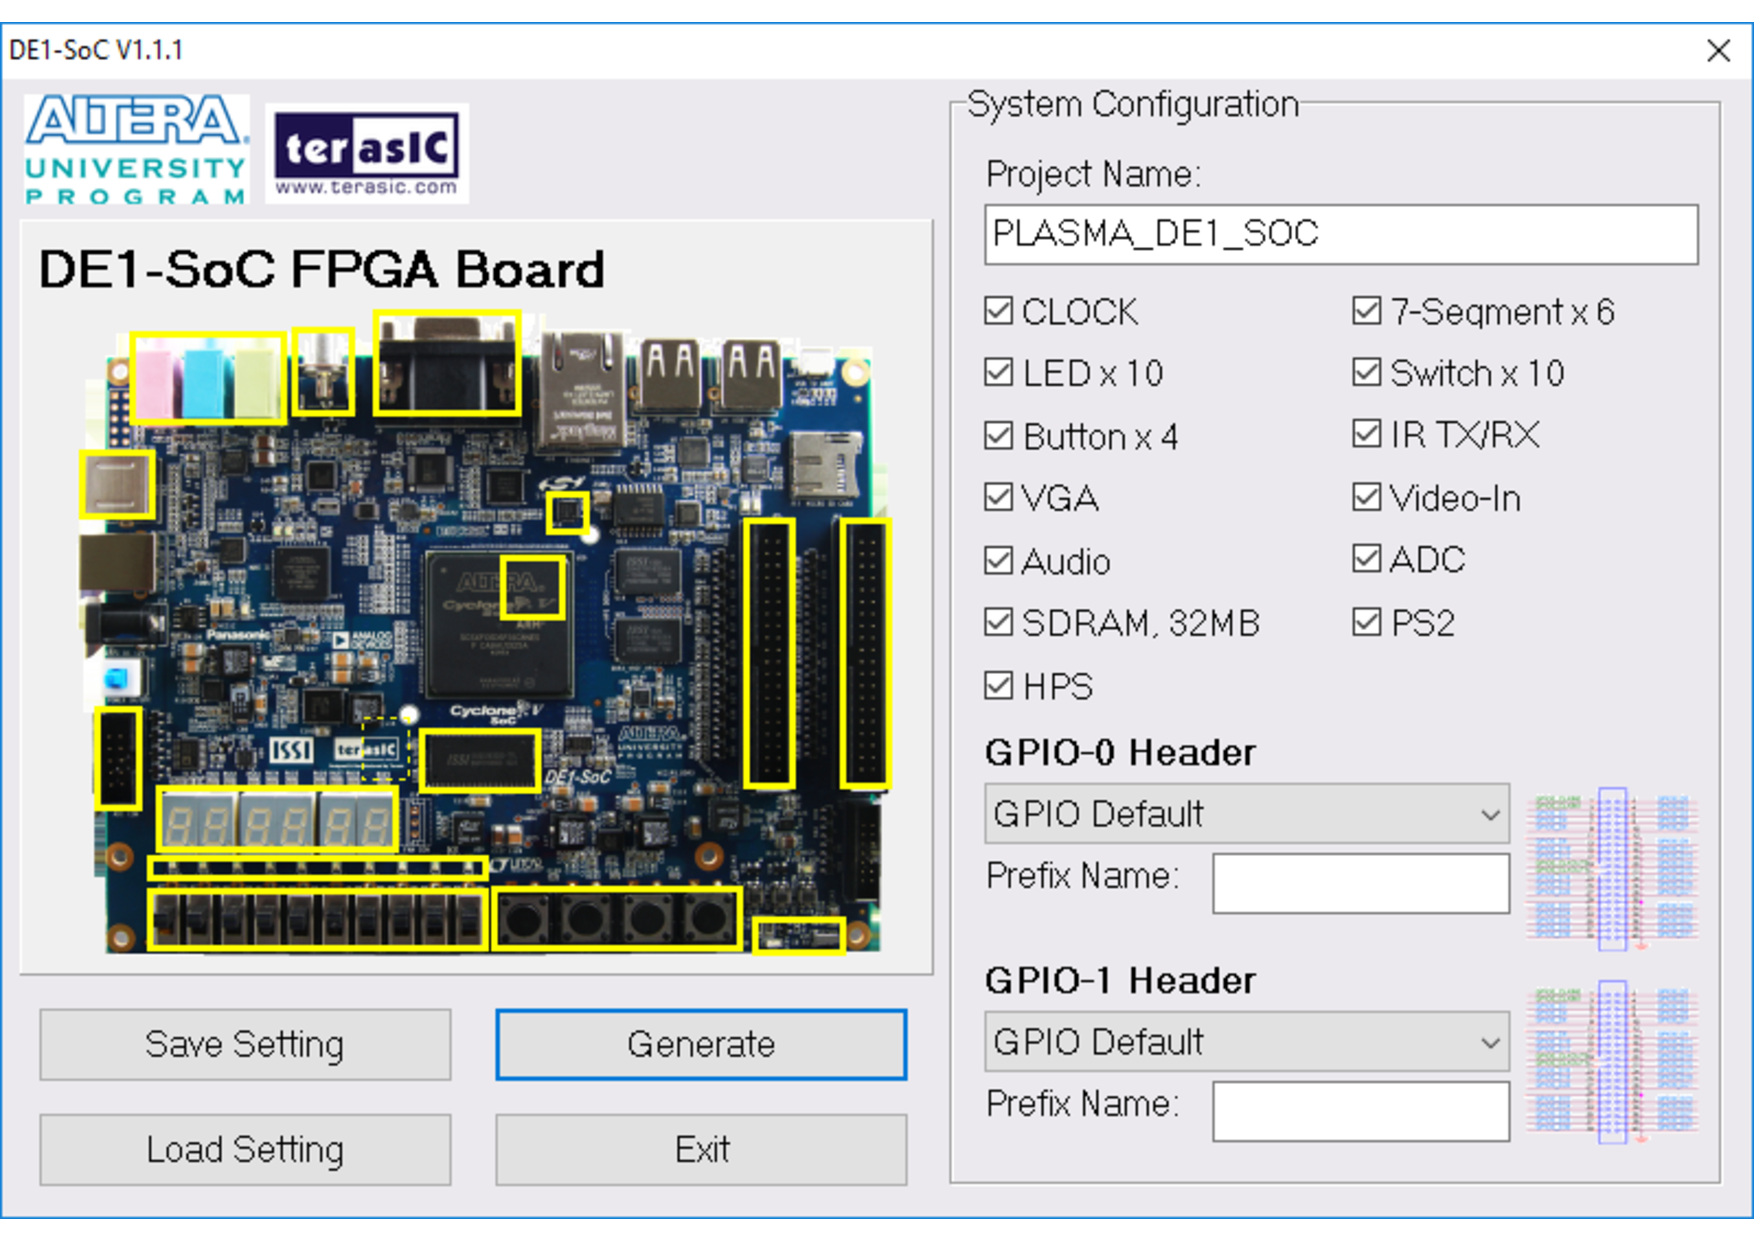
\includegraphics[width=0.6\linewidth]{images/de1_soc_systembuilder}
	\caption{DE1-SoC SystemBuilder}
	\label{fig:de1_soc_systembuilder}
\end{figure}

In der Top-Level-Entity werden die Signalzuordnungen für VGA, Audio, Video, Infrarotsender, A/D Wandler und PS2 auskommentiert, da sie nicht gebraucht werden. 
\alertinfo{Die aktuelle Revision des Entwicklungsboards hat bereits einen \SI{64}{\mega\byte} {SDRAM}-Chip verbaut, die Angabe im SystemBuilder (\SI{32}{\mega\byte} {SDRAM}) wurde allem Anschein nach nicht aktualisiert.}

 Im zweiten Schritt wird das Quartus-Projekt überprüft und die tatsächliche Zielplattform zugewiesen, wie auf \cref{fig:quartus_device_settings} dargestellt. 

\begin{figure}[!htbp]
	\centering
	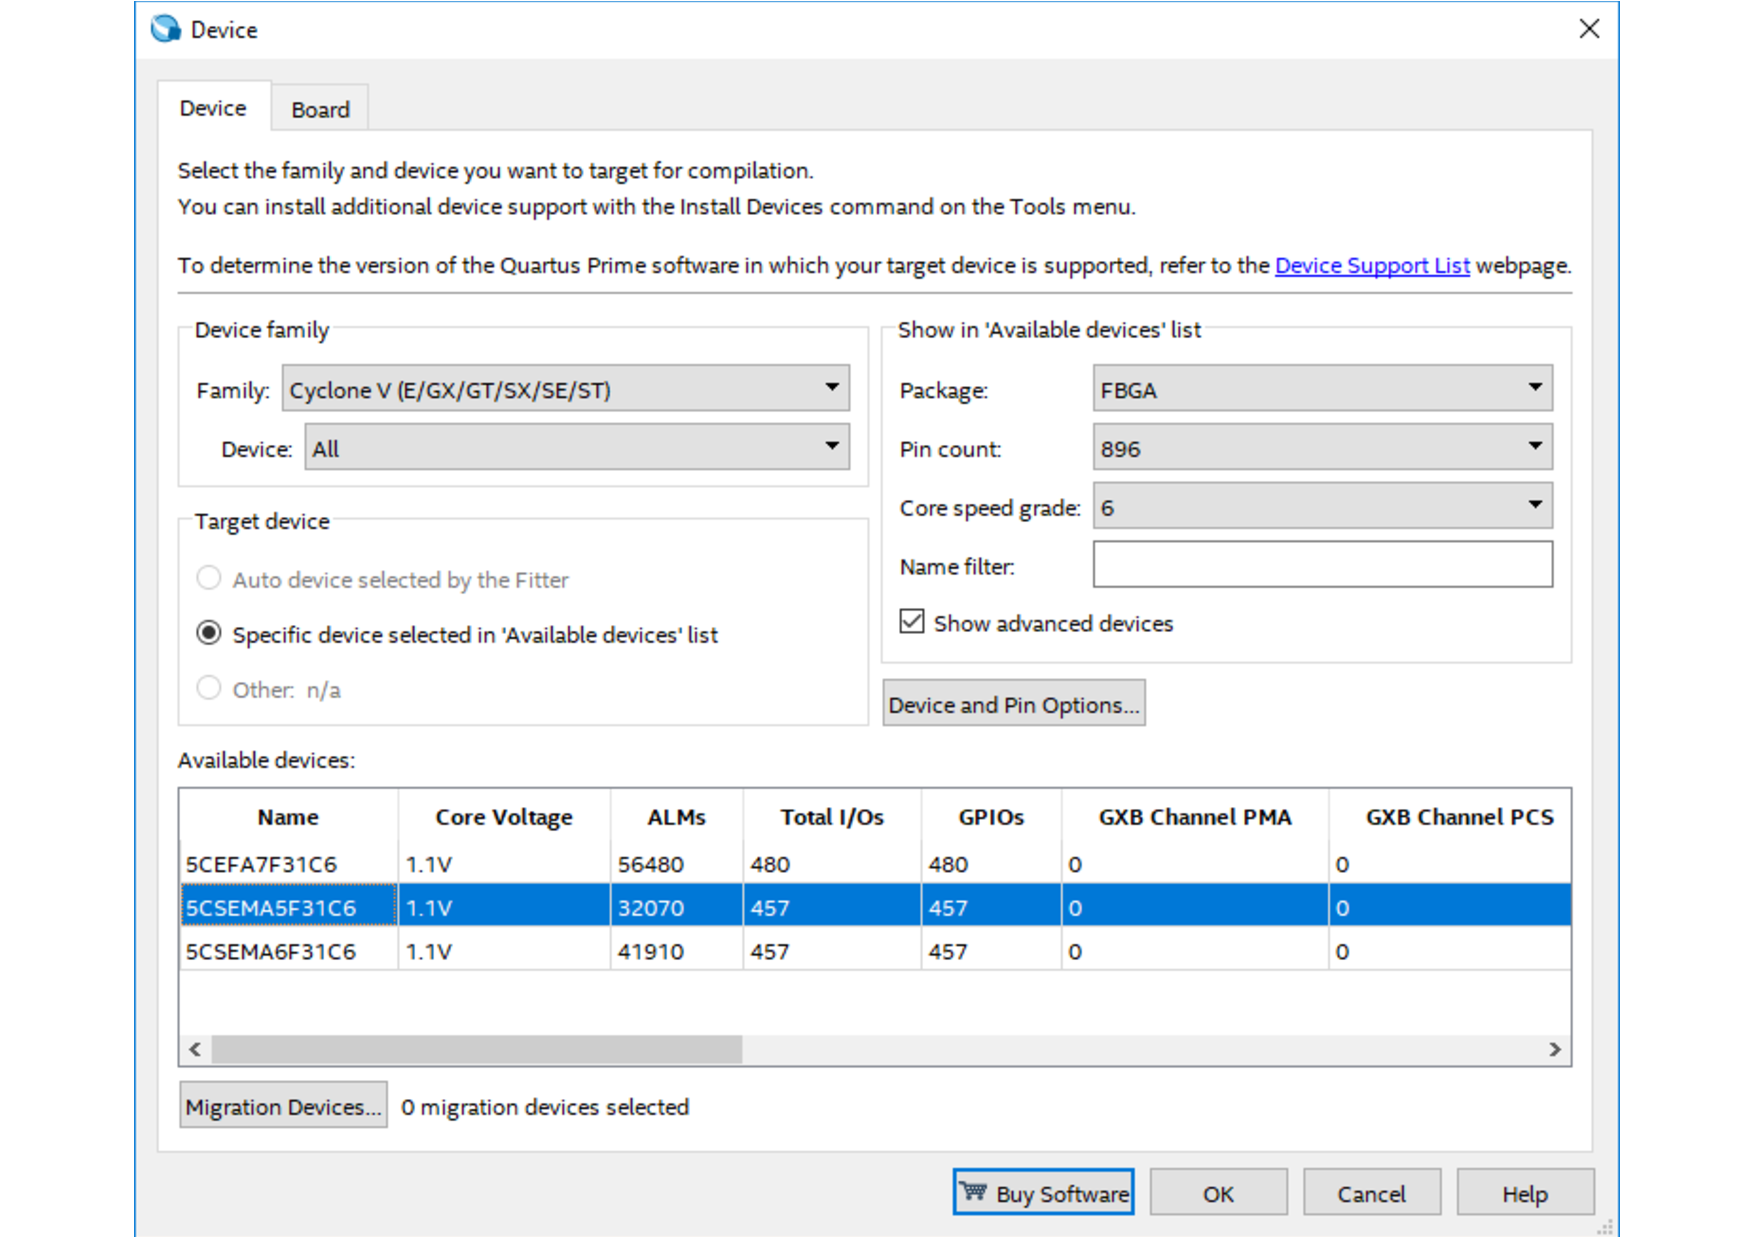
\includegraphics[width=0.6\linewidth]{images/quartus_device_settings}
	\caption{Quartus Boardeinstellungen}
	\label{fig:quartus_device_settings}
\end{figure}


Darauffolgend wird der Platform Designer aufgerufen und über \textit{File \textrightarrow New Component} ein neuer IP-Core erstellt. 
In \cref{fig:plasma_soc_ip_core} wird die Konfiguration für den Plasma-SoC IP-Core gezeigt.

\begin{figure}[!htbp]
	\centering
	\begin{subfigure}{.5\textwidth}
		\centering
		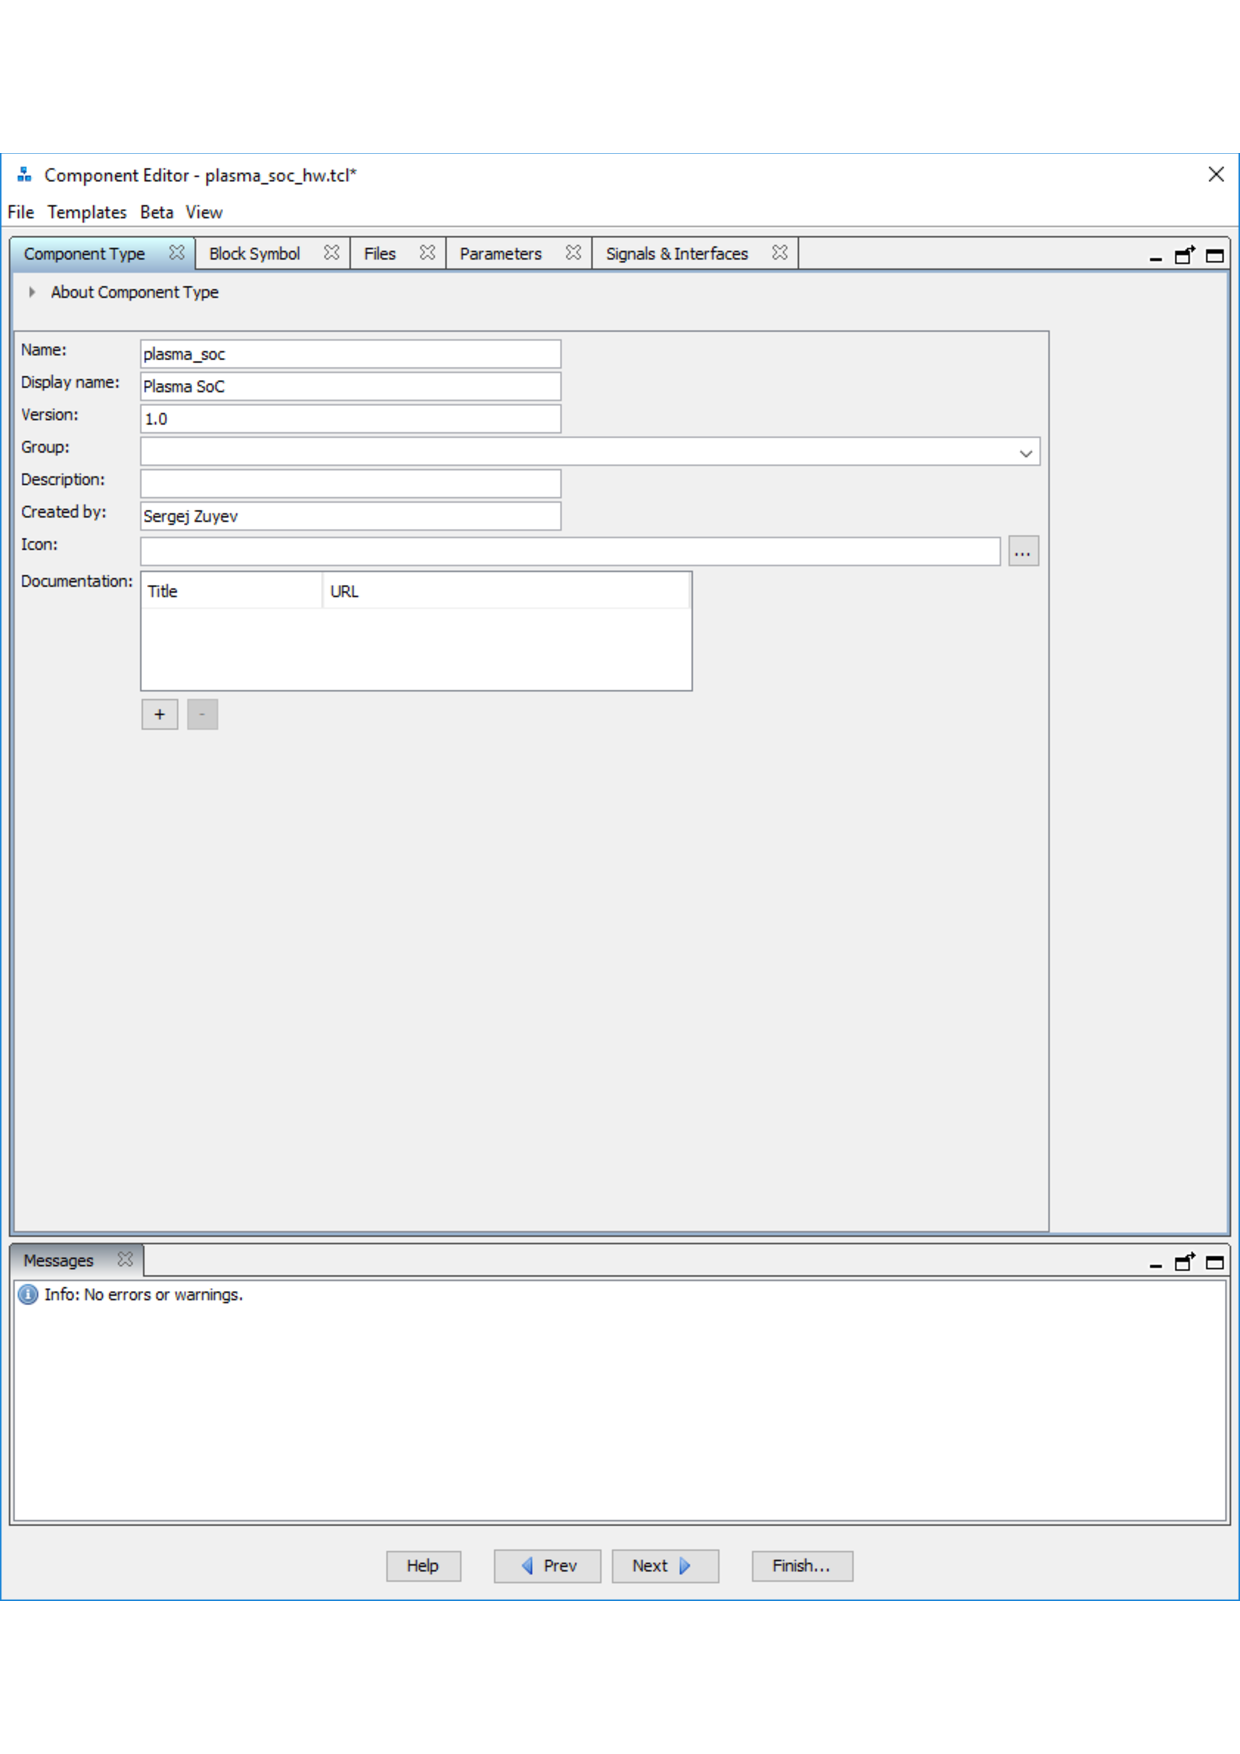
\includegraphics[width=0.9\linewidth]{images/plasma_soc_ip_core_basic}
		\caption{Grundeinstellungen}
		\label{fig:plasma_soc_ip_core_basic}
	\end{subfigure}%
	\begin{subfigure}{.5\textwidth}
		\centering
		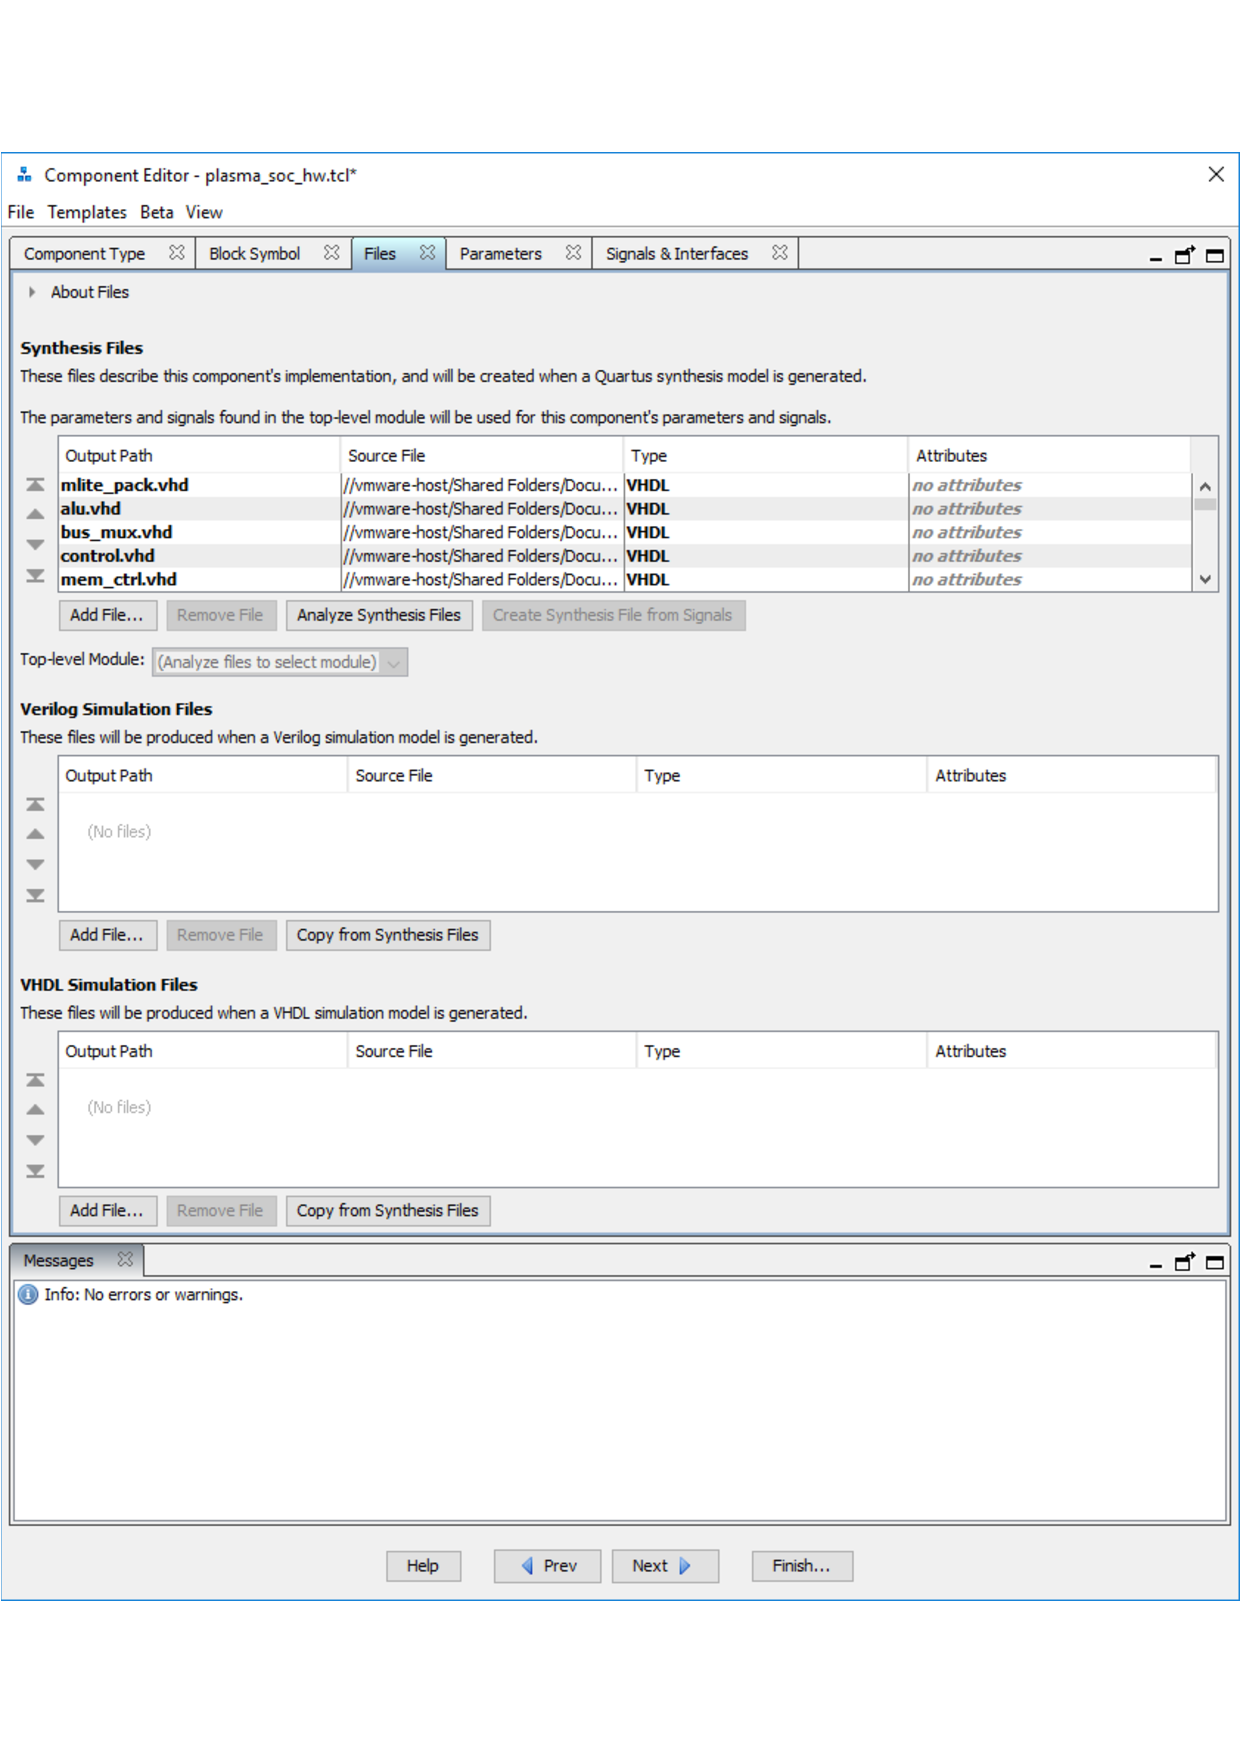
\includegraphics[width=0.9\linewidth]{images/plasma_soc_ip_core_files.pdf}
		\caption{Quelldateien}
		\label{fig:plasma_soc_ip_core_files}
	\end{subfigure}
	\caption{Plasma-\gls{SoC} IP-Core}
	\label{fig:plasma_soc_ip_core}
\end{figure}

Leider kann ein mit dem Platform Designer erstelltes System nicht in Modelsim simuliert werden. Die Ursache dafür ist unklar. Darum wird ein neues Projekt \enquote{quartus\_no\_qsys} angelegt, welches ausschließlich das Plasma-System ohne QSYS-Komponenten beinhaltet und Simulationszwecken dient. 


\subsection{RAM}
Im bestehenden System werden Xilinx-Spezifische \gls{RAM}-Blöcke verwendet, dabei sind mehrere \gls{RAM}-Typen für Altera bzw. Xilinx konfigurierbar. Es gilt, eine passende Variante für den Altera-\glspl{FPGA} zu finden. 

Dabei wird zunächst versucht, den \gls{RAM} über \gls{Inferring} zu implementieren. Dieses Verfahren erweist sich jedoch als ungeeignet, da bei der Synthese der gesamte im Entwicklersystem verfügbare Arbeitsspeicher inkl. Swap aufgebraucht wird:

\begin{minted}[breaklines, autogobble]{text}
Error (114016): Out of memory in module quartus\_map.exe (24430 megabytes used)

Error (114016): Out of memory in module quartus\_map.exe (44107 megabytes used) 
\end{minted}

Als Nächstes werden die Altera \Gls{LPM} Bausteine untersucht. Die Synthese verläuft zwar erfolgreich, jedoch wird das Beispielprogramm nicht ausgeführt. Quartus bietet mit dem In-System Memory Content Editor \cite{manual:memedit} eine Möglichkeit, den Speicherinhalt zu überprüfen und ggf. zu modifizieren. Dazu muss der \gls{LPM}-\gls{RAM}-Instanziierung ein zusätzliches Parameter hinzugefügt werden: \textit{lpm\_hint => \enquote{ENABLE\_RUNTIME\_MOD = YES, INSTANCE\_NAME = <instantiation name>}} \cite[15-2]{manual:memedit}.

Ein weiterer wichtiger Aspekt ist die Initialisierung des Speichers. Der Speicher kann unter Anderem mit einer \Gls{MIF}-Datei (\textbf{.mif}) oder Hexadecimal (Intel-format) Datei (\textbf{.hex}) initialisiert werden \cite[4-18]{manual:ug_ram}. Der Pfad zur Initialisierungsdatei wird im Parameter \textit{LPM\_FILE} angegeben. Verwendet wird in dieser Bachelorarbeit das MIF-Format; Details werden im \cref{sec:impl_extend_tools_for_de1_soc} beschrieben. 

 Nach einem erneuten Testlauf stürzt der Memory Content Editor beim Versuch, den Speicherinhalt zu Laden, ab. Auffällig ist, dass die Blocktiefe 0 beträgt, wie in \cref{fig:quartus_memedit_fail} zu sehen ist. Dieser Wert ist ungültig \cite[4-9]{manual:ug_ram} und muss korrigiert werden. Aus dem Synthese-Log ergibt sich der zu setzende Parameter \textit{LPM\_NUMWORDS}:

\begin{minted}[breaklines, highlightlines=4, autogobble]{text}
	Info (12133): Instantiated megafunction (...) with the following parameter:	
	Info (12134): Parameter "LPM_WIDTH" = "8"	
	Info (12134): Parameter "LPM_WIDTHAD" = "11"	
	Info (12134): Parameter "LPM_NUMWORDS" = "0"	
	Info (12134): Parameter "LPM_INDATA" = "REGISTERED"	
	Info (12134): Parameter "LPM_ADDRESS_CONTROL" = "REGISTERED"	
	Info (12134): Parameter "LPM_OUTDATA" = "UNREGISTERED"	
	Info (12134): Parameter "LPM_FILE" = "../../build/sw/examples/sample_ram_image.vhd_block_1.mif"	
	Info (12134): Parameter "LPM_TYPE" = "LPM_RAM_DQ"	
	Info (12134): Parameter "USE_EAB" = "ON"	
	Info (12134): Parameter "INTENDED_DEVICE_FAMILY" = "UNUSED"
	Info (12134): Parameter "LPM_HINT" = "ENABLE_RUNTIME_MOD = YES, INSTANCE_NAME = RAM1"
\end{minted}


Nach der Parametrisierung des Speichers ist der Inhalt vorhanden und auslesbar, wie in \cref{fig:quartus_memedit} dargestellt.  

\begin{figure}[!htbp]
	\centering
	\begin{subfigure}{.5\textwidth}
		\centering
		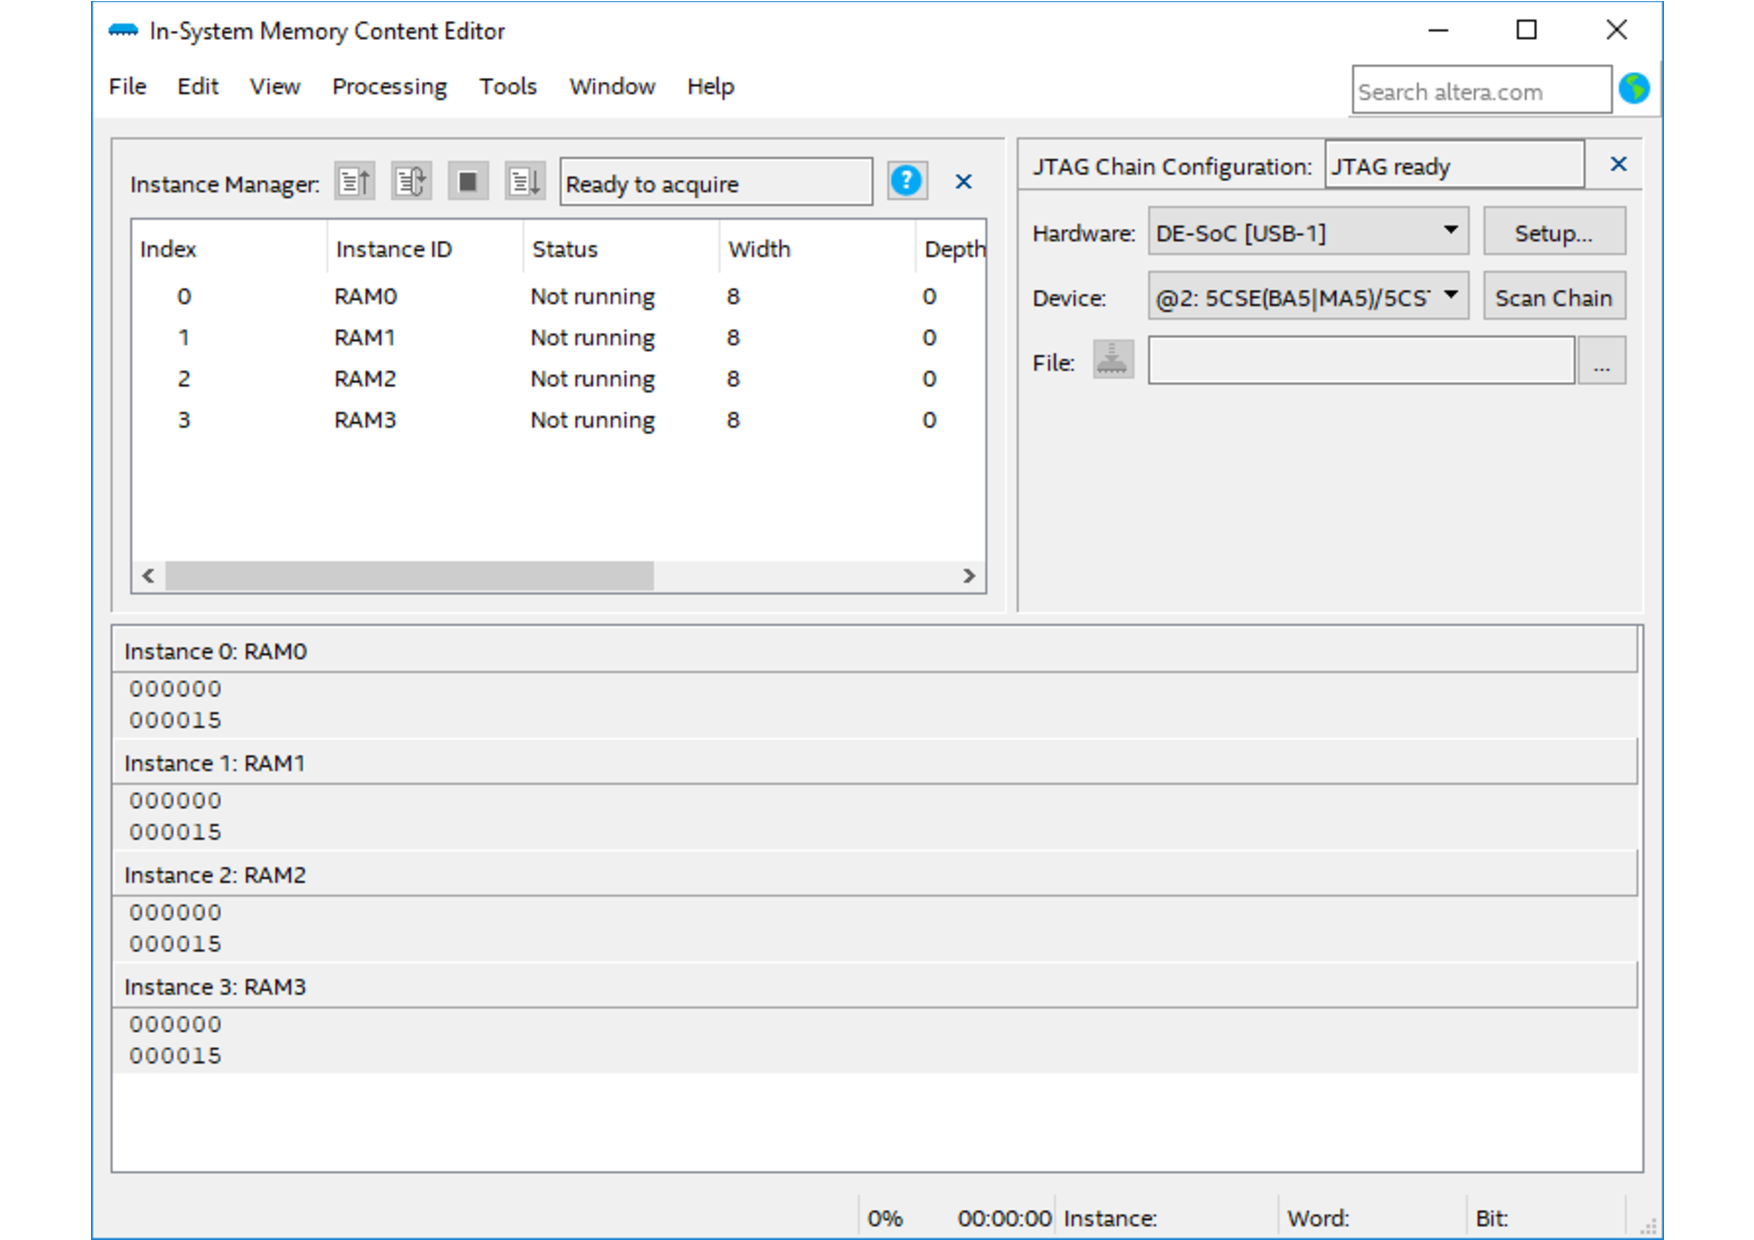
\includegraphics[width=.9\linewidth]{images/quartus_memedit_fail}
		\caption{Fehlerhafte LPM-Parametrisierung}
		\label{fig:quartus_memedit_fail}
	\end{subfigure}%
	\begin{subfigure}{.5\textwidth}
		\centering
		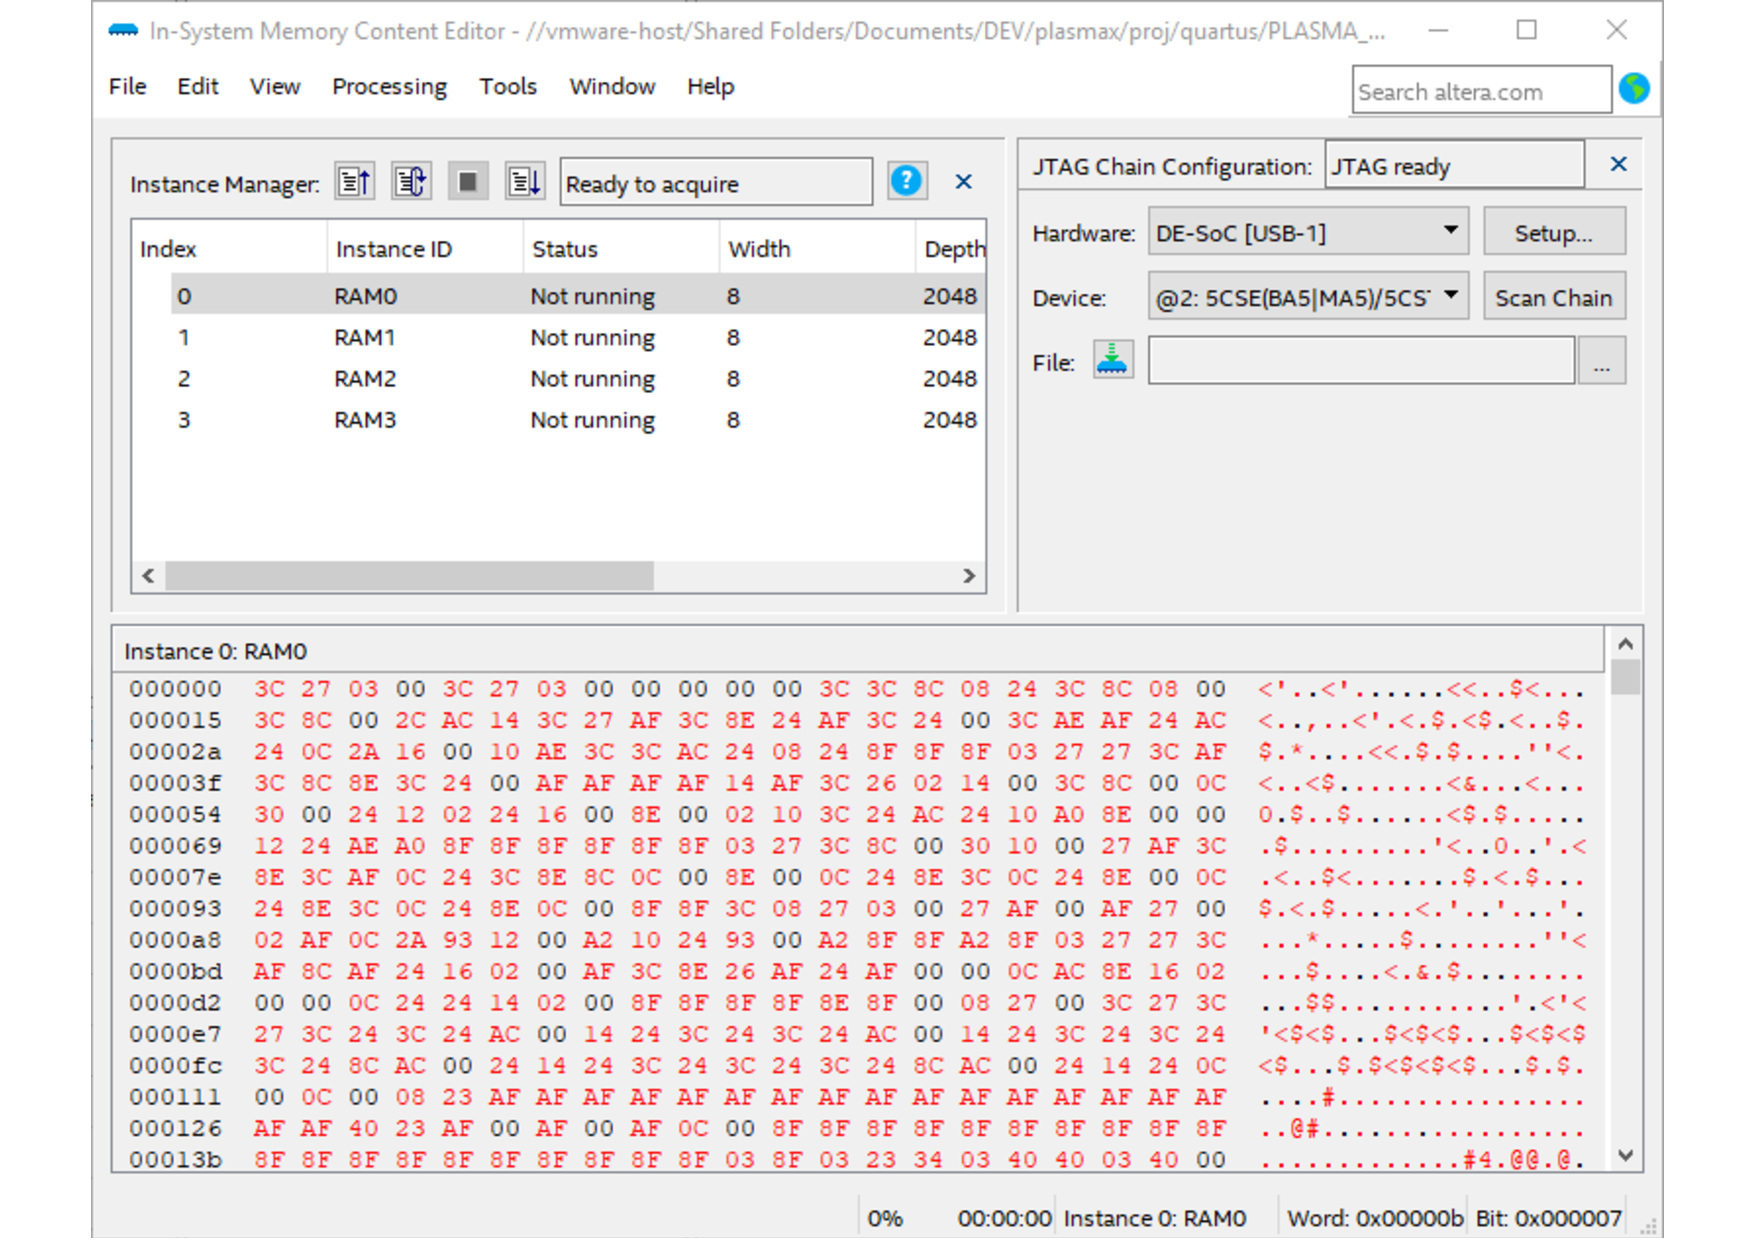
\includegraphics[width=.9\linewidth]{images/quartus_memedit}
		\caption{Korrekte LPM-Parametrisierung}
		\label{fig:quartus_memedit}
	\end{subfigure}
	\caption{Ausgelesener Speicherinhalt}
	\label{fig:cmp_mem_impl}
\end{figure}

\subsection{Register-File}
Das Beispielprogramm wird dennoch nicht ausgeführt. Die Vermutung, dass das als \gls{RAM}-Block implementierte Register-File nicht synthetisiert wird, bestätigt sich durch eine Überprüfung der generierten Netzliste im RTL-Viewer. In \cref{fig:cmp_mem_reg_bank} sind die Netzlisten des Arbeitsspeichers und der Register-Datei gegenübergestellt. Während in \cref{fig:slave_mem_schematics} die \gls{LPM}-\gls{RAM}-Elemente deutlich zu sehen sind, ist im Register-File auf \cref{fig:reg_bank_schematics} nur Steuerlogik ohne \gls{RAM}-Blöcke erkennbar. 

\begin{figure}[!htbp]
	\centering
	\begin{subfigure}{.5\textwidth}
		\centering
		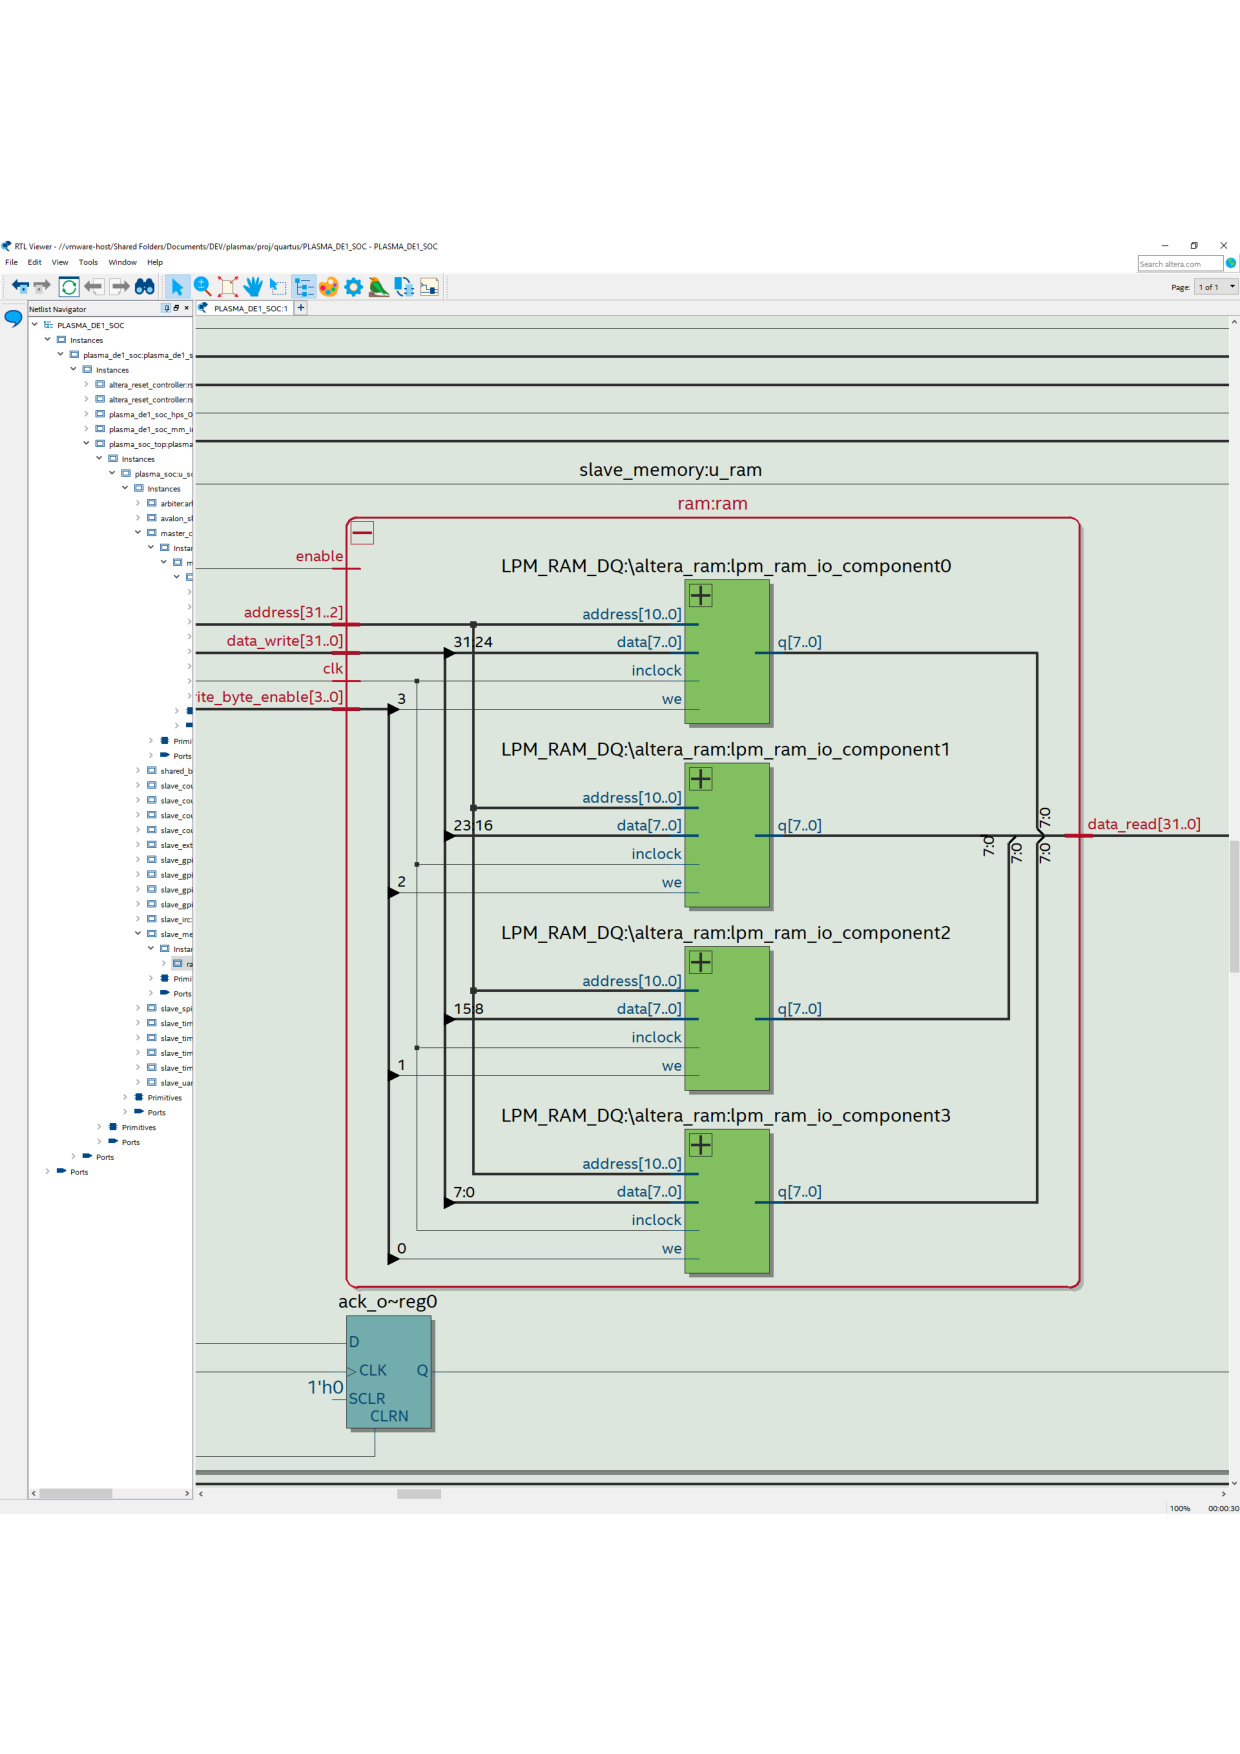
\includegraphics[width=.9\linewidth]{images/slave_mem_schematics}
		\caption{RAM}
		\label{fig:slave_mem_schematics}
	\end{subfigure}%
	\begin{subfigure}{.5\textwidth}
		\centering
		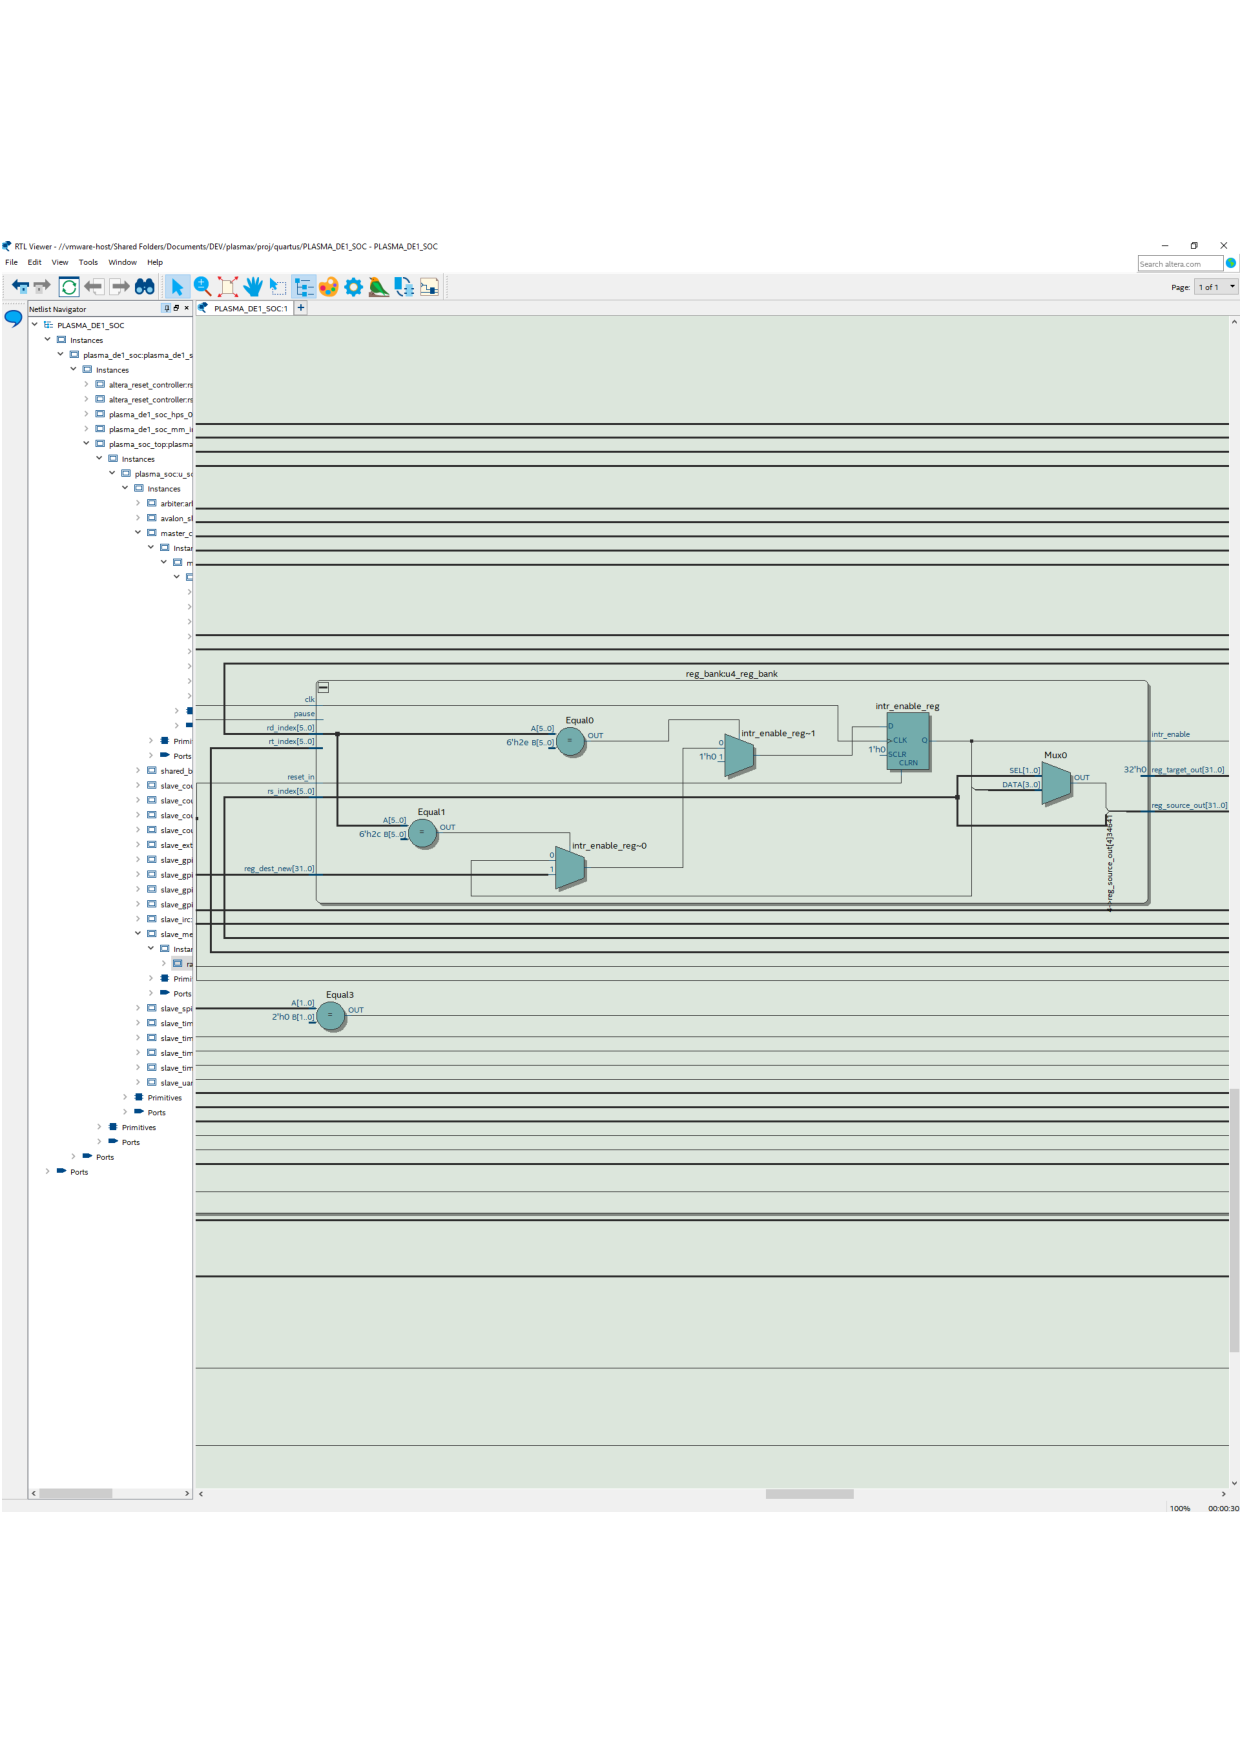
\includegraphics[width=.9\linewidth]{images/reg_bank_schematics}
		\caption{REG\_BANK}
		\label{fig:reg_bank_schematics}
	\end{subfigure}
	\caption{Vergleich der RTL-Netzlisten}
	\label{fig:cmp_mem_reg_bank}
\end{figure}

Es stellt sich heraus, dass für die Register-Datei der Speichertyp-Parameter mit dem ungeeigneten Wert \enquote{XILINX\_16X} konfiguriert ist und die Register-Datei deswegen nicht synthetisiert wird. Altera \gls{LPM}-\gls{RAM}-Blöcke erweisen sich ebenfalls als ungeeignet, da sie mit dem verwendeten Cyclone V \gls{FPGA} inkompatibel sind:

\begin{minted}[breaklines, autogobble]{text}
Warning (272007): DUAL PORT RAM for Cyclone V not possible with the altsyncram megafunction. Implementing using benchmarking mode, trying to tie up the inputs using available clocks. Output behavior will not be the same

Error (287078): Assertion error: Can't convert dual-port RAM for Cyclone V device family using altsyncram megafunction because Cyclone V supports only synchronous dual-port RAM
\end{minted}

Es wird ein durch \gls{Inferring} synthetisierbarer Tri-Port Speicher mit zwei Lese- und einem Schreibport für die Register-Datei ausgewählt. 

\subsection{Laufzeitverhalten}
Durch Prüfung des Speicherinhalts während der Simulation fällt eine unsaktionierte Änderung des Arbeitsspeichers auf. Eine weitreichende Analyse zeigt, dass die Umsetzung des Arbeitsspeichers das vom Wishbone-Wrapper aus dem \textit{STB}-Signal generierte \textit{enable}-Signal nicht nutzt. Dies hat zur Folge, dass bei einem Schreibzugriff auf einen beliebigen Wishbone-Slave der auf dem Datenbus anliegende Wert in den Speicher übernommen wird. Nach der Behebung dieses Fehlers wird das Beispielprogramm korrekt ausgeführt und die im nächsten Abschnitt beschriebene Erweiterung der Hardware beginnt.

\section{Erweiterung der Hardware für DE1-SoC}
\label{sec:impl_extend_hw_for_de1_soc}

\subsection{Avalon-Wishbone Bridge}

Wie bereits im \cref{sec:theory_avalon} erwähnt, nutzt ein vom Platfom Designer generiertes \gls{SoC} den proprietären Avalon-\gls{Interconnect}. Das Plasma-\gls{SoC} hingegen setzt den Wishbone-\gls{Interconnect} ein. Damit beide Systeme sinnvoll verknüpft werden können, bedarf es einer Wishbone{$\leftrightarrow$}Avalon-\gls{Bridge}. 

In \cref{tab:avalonmm_wishbone_comparison} ist eine Gegenüberstellung der wichtigsten Avalon-MM und Wishbone Schnittstellensignale dargestellt. Erkennbar ist, dass Takt-, Adress- und Datensignale, sowie die Steuersignale zum Großteil 1:1 zugeordnet werden können \cite{article:porting_from_wb_to_avalon}. Das \textit{chipselect}-Signal gilt als veraltet \cite[Appendix A]{manual:avalon_spec}. Darum werden die Zuordnungen zu den Steuersignalen wie \textit{cyc\_i}, \textit{stb\_i} und \textit{we\_i} durch kombinatorische Logik und Zustandsautomaten hergeleitet. Die Timingdiagramme sind jeweils für die Avalon\textrightarrow{}Wishbone- und Wishbone\textrightarrow{}Avalon-Bridge in \cref{fig:timing_avalon_wb_bridge} und \cref{fig:timing_wb_avalon_bridge} abgebildet.

\begin{table}[!htbp]
	\bigskip
	\centering
	\begin{tabular}{ | l | l | }
		\hline
	    \textbf{Wishbone Bus} & \textbf{Avalon-MM} \\
	    \hline
 	    {clk\_i} & {clk} \\
 	    \hline
  	    {rst\_i} & {reset\_n} \\
  	    \hline
  	    {cyc\_i} & {read \textit{or} write} \\
  	    \hline
  	    {stb\_i} & {chipselect bzw. read \textit{or} write} \\
  	    \hline
     	{we\_i} & {write \textit{and not} read} \\
  	    \hline
  	    {sel\_i} & {byteenable} \\
  	    \hline
  	    {adr\_i} & {address} \\
  	    \hline
	    {dat\_i} & {readdata} \\
	    \hline
   	    {dat\_o} & {writedata} \\
   	    \hline
   	    {ack\_o} & {waitrequest\_n} \\
		\hline
	\end{tabular}
	
	\caption{Avalon-MM und Wishbone Schnittstellen}
	\label{tab:avalonmm_wishbone_comparison}
\end{table}


\begin{figure}[!htbp]
	\centering
	\begin{subfigure}{\textwidth}
		\centering
		\begin{tikztimingtable} [xscale=1.5,yscale=0.9]
			clk      & [C]24{C} \\
			\\
			address                          & 10D{0} 2U 10D{10} 2U\\
			byteenable              & 10D{F} 2U 10D{F} 2U \\
			read              & 10H 2L 12L \\
			write              & 12L 10H 2L \\
			readdata        &  8U 2D{FF} 2U 12U\\
			writedata              & 12U 10D{EE} 2U \\
			waitrequest\_n              & 8L 2H 2L 8L 2H 2L \\
			response              & 8D{}2D{}2D 8D{}2D{}2D \\
			\\ % Gives vertical space
			cyc\_o     & 2L 8H 2L 2L 8H 2L\\
			stb\_o     & 2L 8H 2L 2L 8H 2L\\
			adr\_o    & 10D{0} 2U 10D{10} 2U\\
			we\_o     & 12L 10H 2L \\
			sel\_o      & 2D{}8D{F}2D{}10D{F}2D \\
			dat\_i 		& 8U 2D{FF} 2U 12U \\
			dat\_o      & 12U 10D{EE} 2U \\
			ack\_i     & 8L 2H 2L 8L 2H 2L\\
			err\_i     & 12L 12L \\			
		\end{tikztimingtable}
		\caption{Avalon\textrightarrow{}Wishbone-Bridge}
		\label{fig:timing_avalon_wb_bridge}
	\end{subfigure}%

	\medskip
	
	\begin{subfigure}{\textwidth}
		\centering
		\begin{tikztimingtable}[xscale=1.5,yscale=0.9]
			clk      & [C]24{C} \\	
			\\ % Gives vertical space
			cyc\_i     & 10H 2L 10H 2L\\
			stb\_i     & 2H 10L 2H 10L\\
			adr\_i    & 10D{0} 2U 10D{10} 2U\\
			we\_i     & 12L 10H 2L \\
			sel\_i      & 10D{F}2D{}10D{F}2D \\
			dat\_i 		& 8U 2D{FF} 2U 12U \\
			dat\_o      & 12U 10D{EE} 2U \\
			ack\_o     & 8L 2H 2L 8L 2H 2L\\
			err\_o     & 12L 12L \\
			\\
			address        & 10D{0} 2U 10D{10} 2U\\
			byteenable   & 10D{F} 2U 10D{F} 2U \\
			read              & 2L 8H 2L 12L \\
			write              & 12L 2L 8H 2L \\
			readdata        &  8U 2D{FF} 2U 12U\\
			writedata        & 12U 10D{EE} 2U \\
			waitrequest\_n  & 8L 2H 2L 8L 2H 2L \\
			response              & 8D{}2D{}2D 8D{}2D{}2D \\
		\end{tikztimingtable}
		\caption{Wishbone\textrightarrow{}Avalon-Bridge}
		\label{fig:timing_wb_avalon_bridge}
	\end{subfigure}
	\caption{Wishbone{$\leftrightarrow$}Avalon-\gls{Bridge} Timings}
	\label{fig:av_wb_timing}
\end{figure}

%\begin{figure}[!htbp]
%	\centering	
%	\begin{tikztimingtable} [xscale=1.5,yscale=0.9]
%		clk      & [C]24{C} \\
%		\\
%		address                          & 10D{0} 2U 10D{10} 2U\\
%		byteenable              & 10D{F} 2U 10D{F} 2U \\
%		read              & 10H 2L 12L \\
%		write              & 12L 10H 2L \\
%		readdata        &  8U 2D{FF} 2U 12U\\
%		writedata              & 12U 10D{EE} 2U \\
%		waitrequest\_n              & 8L 2H 2L 8L 2H 2L \\
%		response              & 8D{}2D{}2D 8D{}2D{}2D \\
%		\\ % Gives vertical space
%		cyc\_o     & 2L 8H 2L 2L 8H 2L\\
%		stb\_o     & 2L 8H 2L 2L 8H 2L\\
%		adr\_o    & 10D{0} 2U 10D{10} 2U\\
%		we\_o     & 12L 10H 2L \\
%		sel\_o      & 2D{}8D{F}2D{}10D{F}2D \\
%		dat\_i 		& 8U 2D{FF} 2U 12U \\
%		dat\_o      & 12U 10D{EE} 2U \\
%		ack\_i     & 8L 2H 2L 8L 2H 2L\\
%		err\_i     & 12L 12L \\			
%	\end{tikztimingtable}
%	\caption{Avalon\textrightarrow{}Wishbone-Bridge Timings}
%	\label{fig:timing_avalon_wb_bridge}
%\end{figure}
%
%\begin{figure}[!htbp]
%	\centering	
%	\begin{tikztimingtable}[xscale=1.5,yscale=0.9]
%		clk      & [C]24{C} \\	
%		\\ % Gives vertical space
%		cyc\_i     & 10H 2L 10H 2L\\
%		stb\_i     & 2H 10L 2H 10L\\
%		adr\_i    & 10D{0} 2U 10D{10} 2U\\
%		we\_i     & 12L 10H 2L \\
%		sel\_i      & 10D{F}2D{}10D{F}2D \\
%		dat\_i 		& 8U 2D{FF} 2U 12U \\
%		dat\_o      & 12U 10D{EE} 2U \\
%		ack\_o     & 8L 2H 2L 8L 2H 2L\\
%		err\_o     & 12L 12L \\
%			\\
%		address        & 10D{0} 2U 10D{10} 2U\\
%		byteenable   & 10D{F} 2U 10D{F} 2U \\
%		read              & 2L 8H 2L 12L \\
%		write              & 12L 2L 8H 2L \\
%		readdata        &  8U 2D{FF} 2U 12U\\
%		writedata        & 12U 10D{EE} 2U \\
%		waitrequest\_n  & 8L 2H 2L 8L 2H 2L \\
%		response              & 8D{}2D{}2D 8D{}2D{}2D \\
%	\end{tikztimingtable}
%	\caption{Wishbone\textrightarrow{}Avalon-Bridge Timings}
%	\label{fig:timing_wb_avalon_bridge}
%\end{figure}

\subsection{Arbiter}

Der bestehende Arbiter ist nicht funktionsfähig. Die Problematik fällt auf dem ZedBoard nicht auf, da der Wishbone-Bus dort mit nur einem Master betrieben wird. Der fehlerhafte Arbiter wird durch einen modifizierten, prioritätsbasierten Round-Robin Arbiter von Benjamin Krill \cite{website:vhdl_round_robin_arbiter} ersetzt.

 Zunächst wird das Zweier-Komplement aus dem Request-Eingangssignal gebildet. Das Ergebnis und das Request-Eingangssignal werden mit dem UND-Operator bitweise verknüpft, wie in \cref{eq:request_lsb} zu sehen ist.  Das Endergebnis hat dann ein \gls{LSB} mit der höchsten Priorität \cite{website:vhdl_round_robin_arbiter}. 

\begin{equation} \label{eq:request_lsb}
	request_{lsb} = request_i \land (\overline{request_i} + 1)	
\end{equation}

In \cref{eq:mask} wird aus dem Request-Eingangssignal und dem gespeicherten vorherigem Grant-Signal eine Maske gebildet, welche dann nach Anwendung der \cref{eq:grant_next} das neue Grant-Signal ergibt \cite{website:vhdl_round_robin_arbiter}.  
\begin{equation} \label{eq:mask}
	mask = request_i \land (\overline{grant_{prev} - 1)  \lor grant_{prev}})
\end{equation}

\begin{equation} \label{eq:grant_next}
	grant_{next} = mask \land (\overline{mask} + 1)
\end{equation}

Anschließend wird in \cref{eq:grant} entweder das neu generierte Grant-Signal bei einer gültigen Maske oder das Request-Signal mit der höchsten Priorität ausgewählt \cite{website:vhdl_round_robin_arbiter}. 
\begin{equation} \label{eq:grant}
	grant = \begin{cases}
		grant_{next}, 	& \text{if } mask \neq 0 \\
		request_{lsb}, 	& \text{otherwise}
		\end{cases}
\end{equation}

Zur Anbindung dieses Arbiters an den Wishbone-Bus wird dieser zusätzlich mit einem One-Hot dekodierten Grant-Signal versehen, da sich  so der entsprechende Master mit den Daten-, Adress- und Steuersignalen einfacher selektieren lässt. Der Wishbone-Wrapper für die \gls{CPU} wird ebenfalls angepasst, sodass die Wishbone-Steuersignale \textit{CYC} und \textit{STB} nur bei einer gültigen Buszuteilung generiert werden.

\subsection{Wishbone-Bus}

Nach der Einführung des verbesserten Arbiters fällt auf, dass die Adresse nach Auswahl des Masters erst einen Taktzyklus später dekodiert anliegt, was zum falschen Betriebsablauf führt. Als Konsequenz wird auf eine mit dem Takt verknüpfte Auswertung und Speicherung im Register verzichtet.

Beim simulationsbasierten Testen der Avalon\textrightarrow{}Wishbone-Bridge, welche als Wishbone-Master fungiert, fällt auf, dass ein vom Slave bereitgestelltes Datenwort erst zwei Taktzyklen nach dem \textit{ACK}-Signal anliegt. Dadurch werden fehlerhafte Werte übernommen.
Um dieses Problem zu umgehen, wird aus dem Wishbone-Bus die letzte an den Takt gebundene Komponente vom Takt enkoppelt. Dadurch verursacht der Bus keine nennenswerte Verzögerung mehr und die Daten liegen zeitgleich an den Ein- und Ausgängen an. Bei höheren Taktfrequenzen könnte es jedoch zu Problemen führen.

Die Plasma-\gls{CPU} erwartet die Daten jedoch immer noch mit einem Taktzyklus Versatz. Darum wird im Wishbone-Wrapper der Plasma-\gls{CPU} ein Register für die Datenleitung hinzugefügt, sodass das aktuell anliegende Datenwort erst einen Takt später zur Verfügung steht. 

\subsection{Externer SDRAM}
\label{sec:external_sdram}
Auf dem DE1-SoC-Board ist ein SDRAM-Chip mit der Modellnummer \texttt{IS42S16320D} von ISSI Technologies verbaut. Dieser fasst \SI{64}{\mega\byte} (32Mx16) und ist mit dem \gls{FPGA} über eine \SI{16}{\bit} breite Datenleitung sowie Kontroll- und Adressleitungen verbunden \cite[38]{manual:de1soc}. Die Grundparameter lassen sich aus \cref{tab:sdram_timings} und \cref{tab:sdram_addresses} entnehmen.

\begin{table}[!htbp]
	\bigskip
	\centering
	\begin{tabular}{ | l | c | c | c | c | }
		\hline
		\textbf{Parameter} & \textbf{-5} &  \textbf{-6} &  \textbf{-7} & \textbf{Einheit} \\
		\hline
		Taktzykluszeit & & & & \\
		\hspace{3mm}\textoverline{CAS} - Latenz = 3 & 5 & 6 & 7 & \SI{}{\nano\second} \\
		\hspace{3mm}\textoverline{CAS} - Latenz = 2 & 10 & 10 & 7.5 & \SI{}{\nano\second} \\
		\hline
		Taktfrequenz & & & & \\
		\hspace{3mm}\textoverline{CAS} - Latenz = 3 & 200& 167 & 143 & \SI{}{\mega\hertz} \\
		\hspace{3mm}\textoverline{CAS} - Latenz = 2 & 100 & 100 & 133 & \SI{}{\mega\hertz} \\
		\hline
		Zugriffszeit & & & & \\
		\hspace{3mm}\textoverline{CAS} - Latenz = 3 & 5.0 & 5.4 & 5.4 & \SI{}{\nano\second} \\
		\hspace{3mm}\textoverline{CAS} - Latenz = 2 & 6 & 6 & 5.4 & \SI{}{\nano\second} \\
		\hline
	\end{tabular}
	\caption{Timing Parameter \cite[1]{manual:issi_sdram}}
	\label{tab:sdram_timings}
\end{table}

\begin{table}[!htbp]
	\bigskip
	\centering
	\begin{tabular}{ | l | l | l | l |}
		\hline
		\textbf{Parameter} & \textbf{16M x 32} & \textbf{32M x 16} & \textbf{64M x 8} \\
		\hline
		Konfiguration & 4M x 32 x 4 banks & 8M x 16 x 4 banks & 16M x 8 x 4 banks\\
		\hline
		Bank Adress Pins & BA0, BA1 & BA0, BA1 & BA0, BA1 \\
		\hline
		Autoprecharge Pins & A10/AP & A10/AP & A10/AP \\
		\hline
		Zeilenadresse & 512(A0 – A8) & 1K(A0 – A9) & 2K(A0 – A9, A11) \\
		\hline
	\end{tabular}	
	\caption{Adresstabelle \cite[1]{manual:issi_sdram}}
	\label{tab:sdram_addresses}
\end{table}

Um den Speicher in Betrieb zu nehmen, ist ein SDRAM-Controller nötig. Dieser steht als IP-Core im Platform Designer zur Verfügung. Folgende Parameter werden mit neuen Werten überschrieben \cite[6]{manual:using_the_sdram}:

\begin{easylist}[itemize]
	& Bits: 16
	& Chip select: 1
	& Banks: 4 (vgl. Konfiguration in \cref{tab:sdram_addresses})
	& Row: 13
	& Column: 10 (vgl. Zeilenadresse in \cref{tab:sdram_addresses})	
\end{easylist}

Die Timings werden ebenfalls angepasst \cite[6]{manual:using_the_sdram}:

\begin{easylist}[itemize]
	& CAS latency cycles: 3
	& Issue one refresh command every: \SI{7.8125}{\micro\second}
	& Duration of refresh command(t\_rp): \SI{15.0}{\nano\second}
	& Duration of precharge command(t\_rcd): \SI{15.0}{\nano\second}
	& Access time(t\_ac): \SI{5.4}{\nano\second} (vgl. Zugriffszeit in \cref{tab:sdram_timings})
\end{easylist}

In \cref{fig:sdram_ctl_params} und \cref{fig:sdram_controller_timings} sind die Parameter im Konfigurationsdialog des SDRAM-Controller-IP-Core abgebildet. 

\begin{figure}[!htbp]
	\centering
	\begin{subfigure}{.5\textwidth}
		\centering
		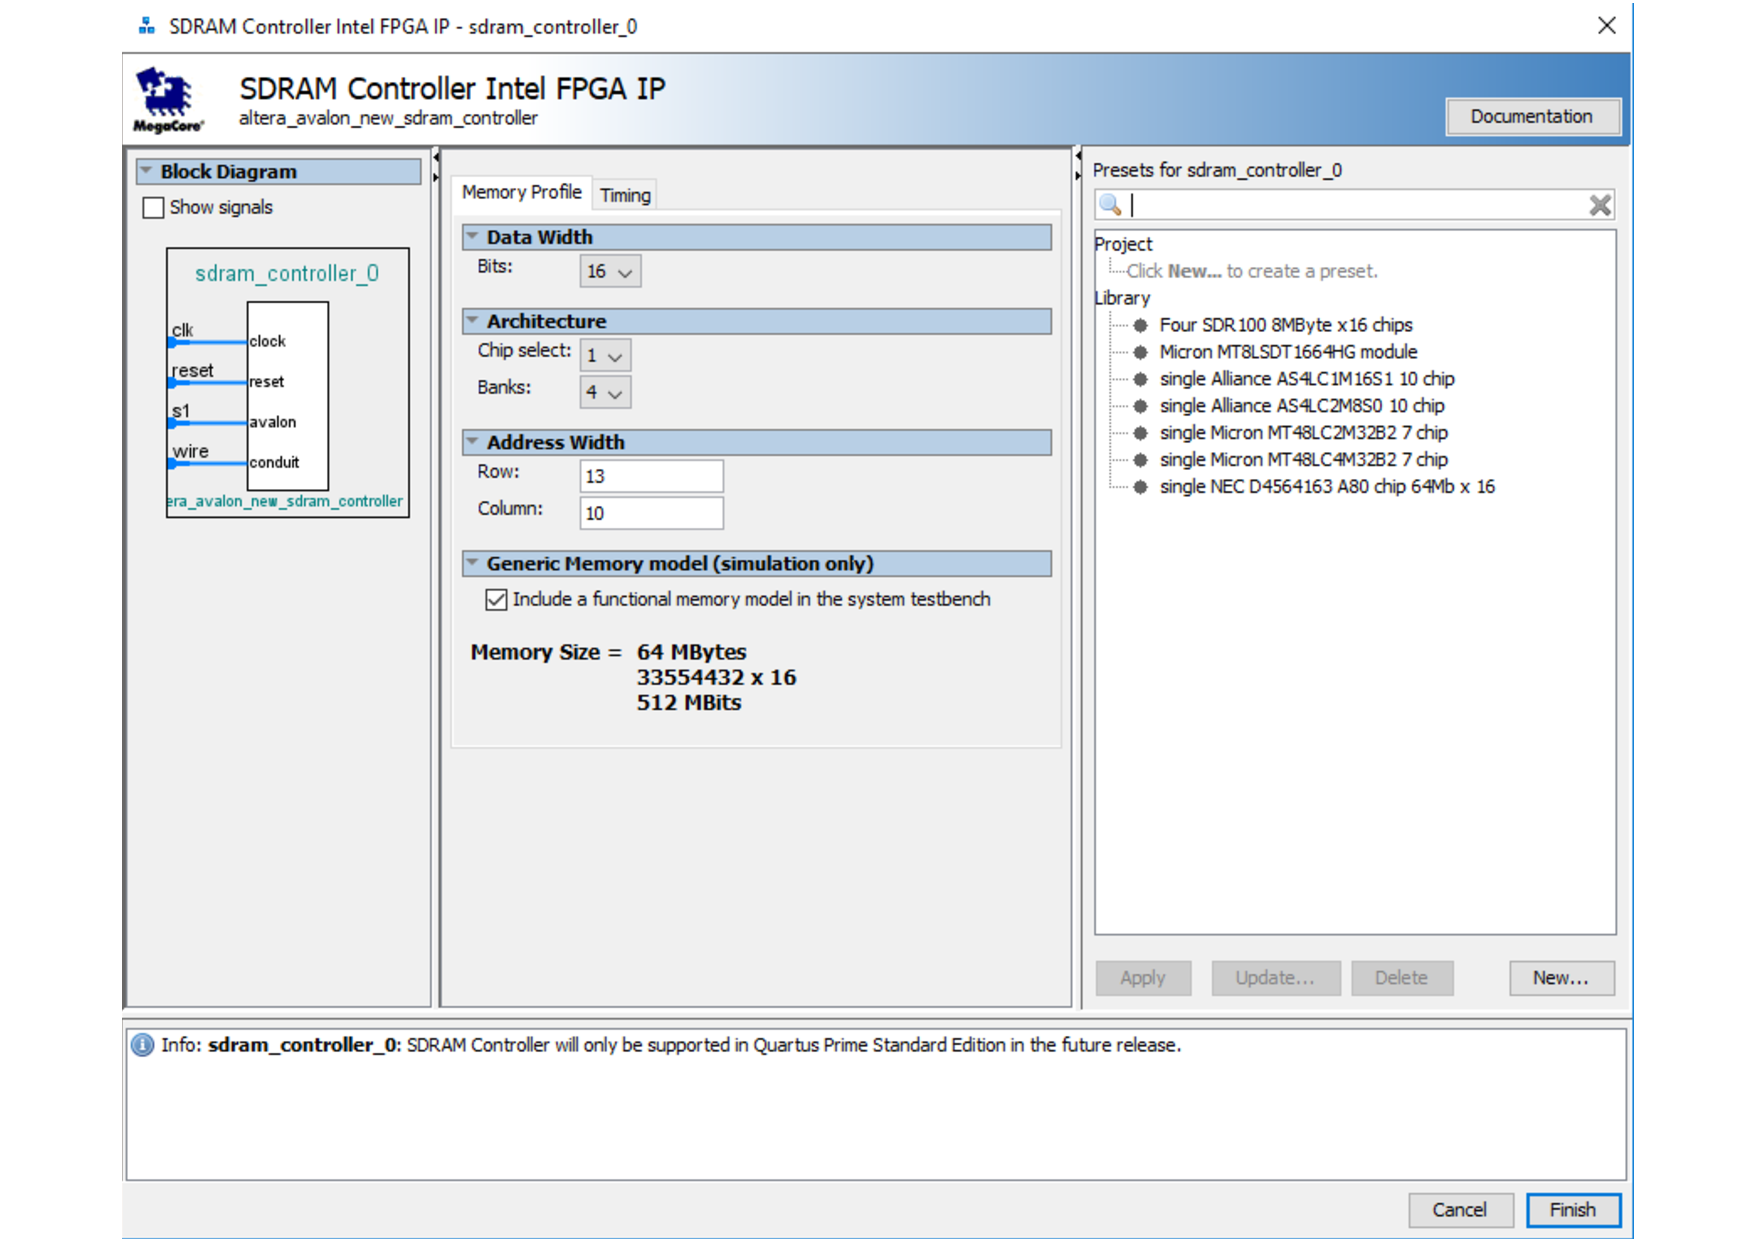
\includegraphics[width=.9\linewidth]{images/sdram_ctl_params.pdf}
		\caption{Allgemeine Parameter}
		\label{fig:sdram_ctl_params}
	\end{subfigure}%
	\begin{subfigure}{.5\textwidth}
		\centering
		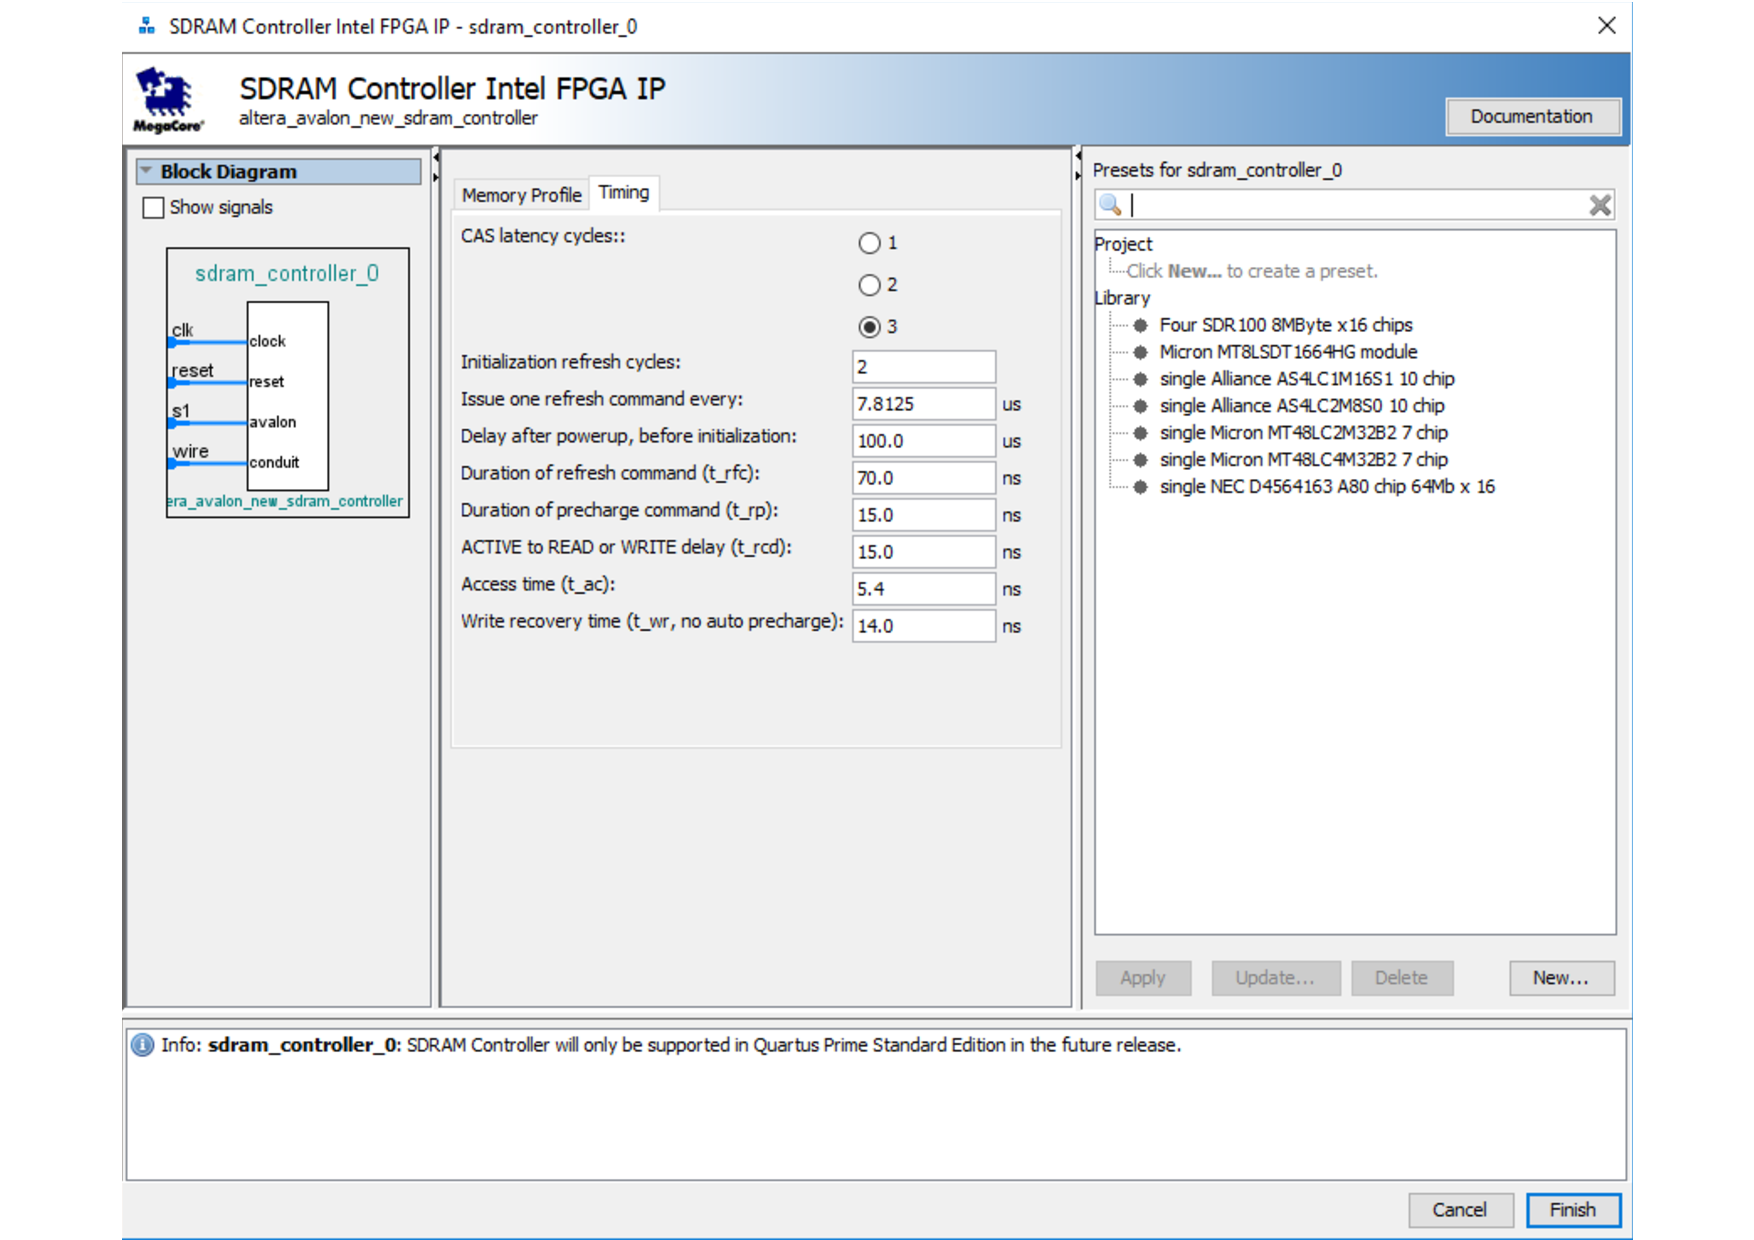
\includegraphics[width=.9\linewidth]{images/sdram_controller_timings.pdf}
		\caption{Timings}
		\label{fig:sdram_controller_timings}
	\end{subfigure}
	\caption{Parametrisierung des SDRAM-Controllers}
	\label{fig:sdram_controller_params}
\end{figure}

Die korrekte Funktion des SDRAM hängt auch von den physikalischen Charakteristika des Boards ab. Unter Anderem hat die Länge der Verbindungsleitungen zwischen dem SDRAM-Chip und dem \gls{FPGA} einen Einfluss auf möglichen Taktversatz. Darum wird eine \gls{PLL} benötigt, die den SDRAM-Takt dem Systemtakt unter Berücksichtigung der physikalischen Parameter um \SI{3}{\nano\second} vorauseilen lässt \cite[13]{manual:using_the_sdram}. 

Dies kann durch Hinzufügen und geeignete Parametrisierung eines \gls{PLL}-IP-Cores oder alternativ durch Hinzufügen des \textit{Clocks Signals for DE-Series Board Peripherals}-IP-Cores geschehen. Die erste Variante setzt eine Berechnung der notwendigen Parameter oder eine aufwändige Analyse mit einem Oszilloskop voraus, sodass die Daten in einem korrekten Zeitfenster anliegen \cite[355ff]{manual:ug_ip_cores}. 

Es wird die zweite Variante gewählt, da sie wesentlich einfacher ist und nur eine Auswahl der Zielhardware im in \cref{fig:sdram_pll_config} dargestellten Konfigurationsdialog erfordert. Es werden der Referenztakt von \SI{50}{\mega\hertz}, der gewünschte Systemtakt von \SI{50}{\mega\hertz} sowie die Zielhardware (das DE1-SoC-Board) eingestellt.

\begin{figure}[!htbp]
	\centering
	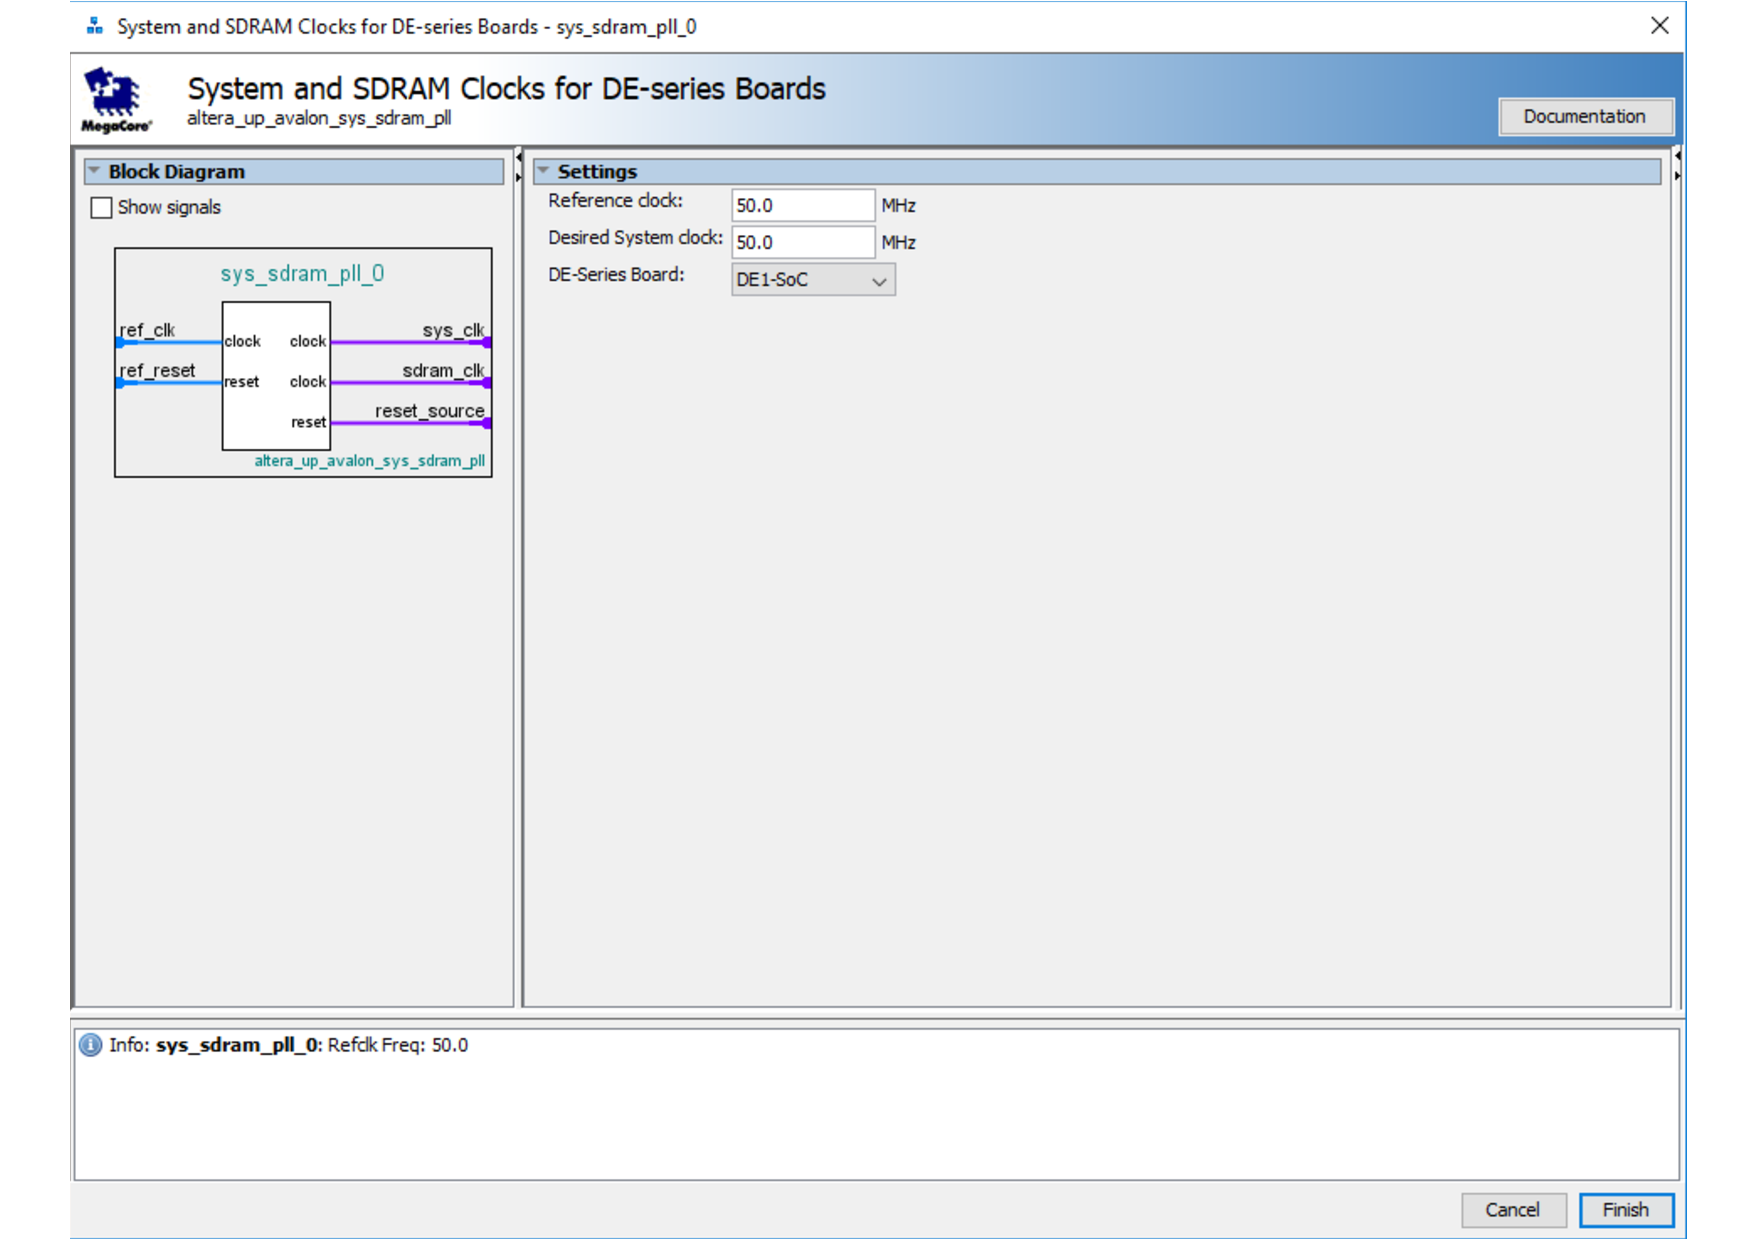
\includegraphics[width=0.6\linewidth]{images/sdram_pll_config}
	\caption{Parametrisierung des \textit{Clocks Signals for DE-Series Board Peripherals}-IP-Core}
	\label{fig:sdram_pll_config}
\end{figure}

Ein wichtiger Aspekt ist, dass der verbaute SDRAM einen \SI{16}{\bit} breiten Datenbus hat. In \cref{fig:sdram_signaltap_waveform} ist ein mit SignalTap aufgezeichneter Zugriff auf den externen SDRAM dargestellt. Von Interesse sind die blau umrahmten Wellenformen für \textit{...|avm\_read} und \textit{...|avm\_waitrequest\_n}. Am oberen Rand der \cref{fig:sdram_signaltap_waveform} ist die Zeit- bzw. Taktleiste zu sehen. Durch Abgleich der Wellenform mit der Zeitleiste lässt sich schlussfolgern, dass der gesamte Lesezyklus 6 Taktzyklen dauert. Da der SDRAM-Controller mit CAS=3 konfiguriert ist, liegen die Daten nach 3 Taktzyklen am Datenbus an. Entsprechend wird ein \SI{32}{\bit} Datenwort aus zwei \SI{16}{\bit} Transfers zusammengesetzt, welche dann zusammen 2x3 Taktzyklen ergeben. 

\begin{figure}[!htbp]
	\centering
	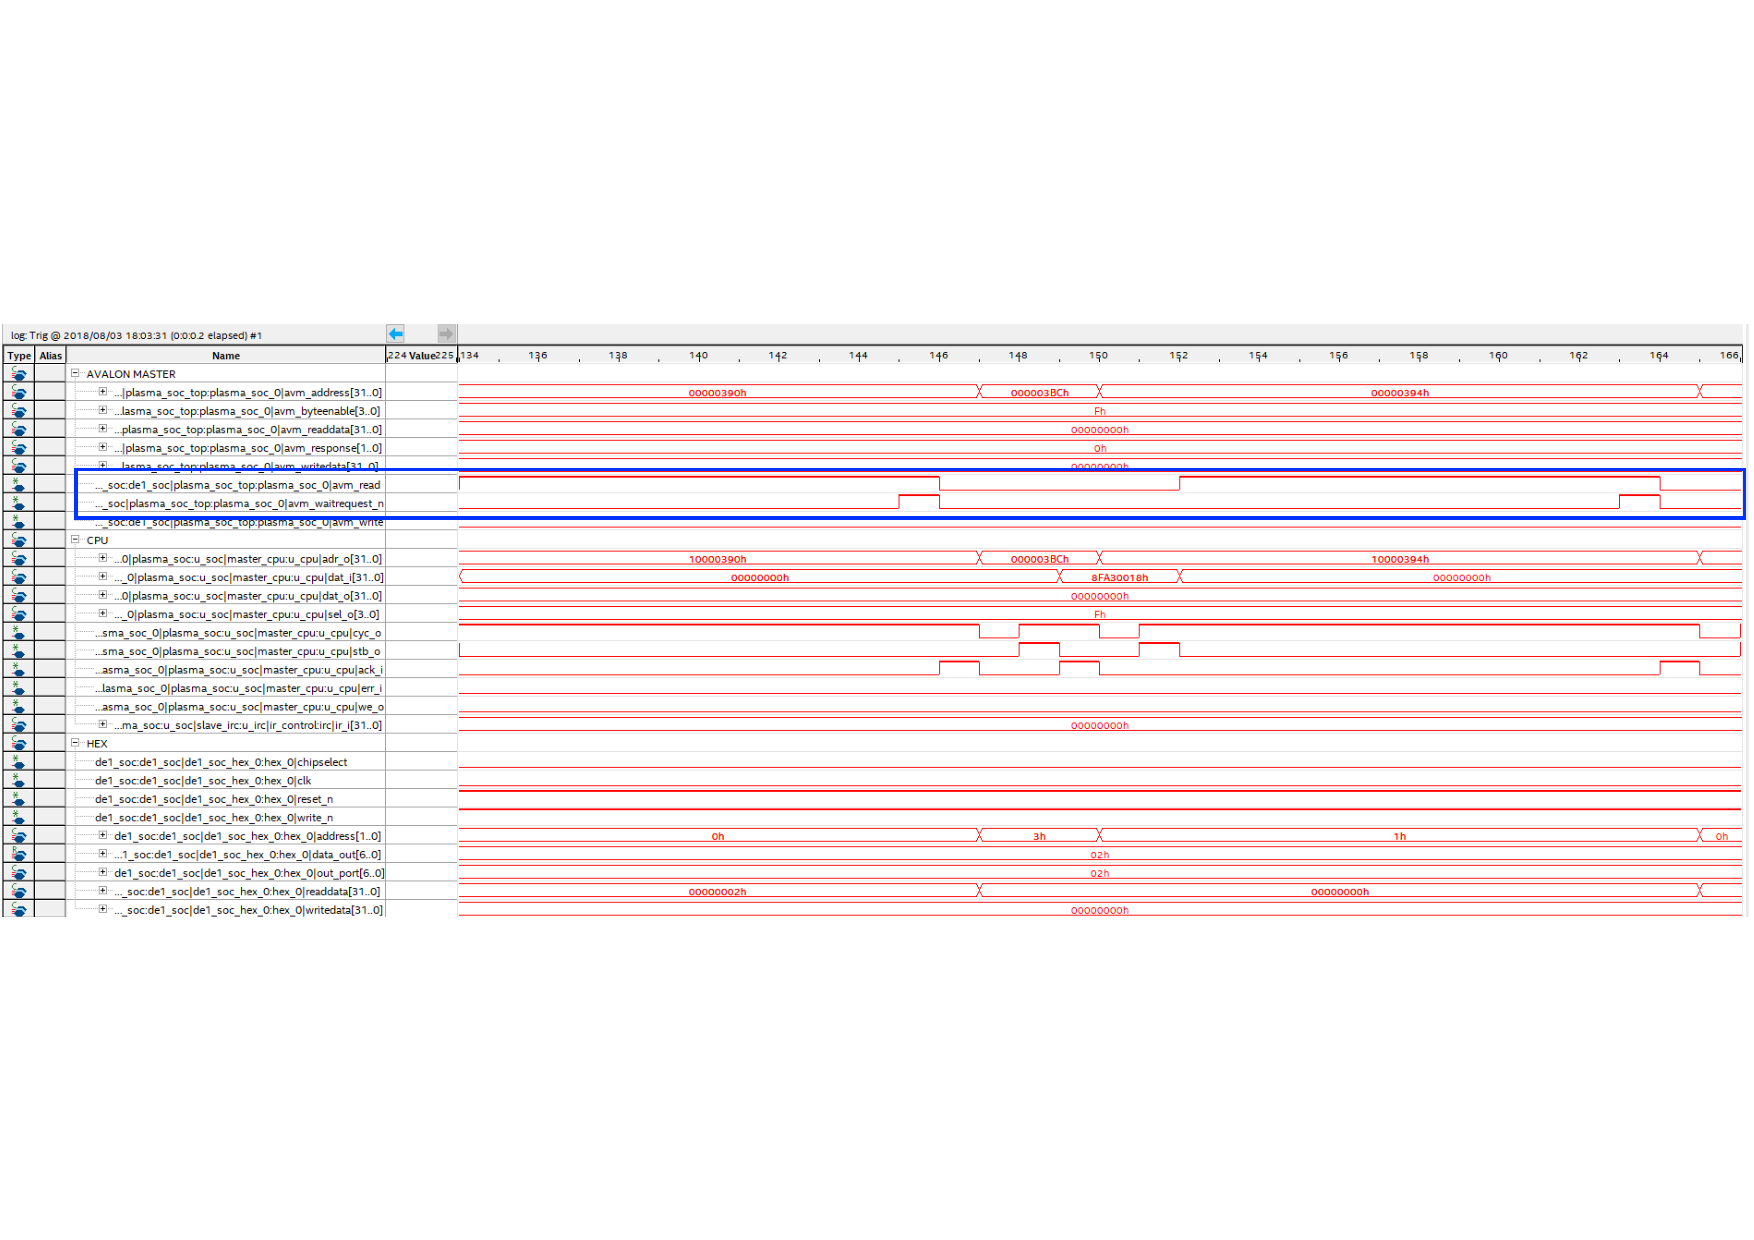
\includegraphics[width=1\linewidth]{images/sdram_signaltap_waveform2}
	\caption{Mit SignalTap aufgezeichneter Zugriff auf den externen SDRAM}
	\label{fig:sdram_signaltap_waveform}
\end{figure}


\subsection{Parallel I/O}

Nach der Fertigstellung der Wishbone{$\leftrightarrow$}Avalon-\gls{Bridge} werden im Platform Designer 8 \gls{PIO}-IP-Cores an die \gls{Bridge} angebunden.

Sechs IP-Cores werden als Ausgänge mit \SI{7}{\bit} Datenbusbreite konfiguriert und mit sechs verfügbaren 7-Segment-Anzeigen verbunden. 

Ein weiterer wird als \SI{10}{\bit}-Eingang konfiguriert und mit dem Schalterblock verbunden, und der letzte wird als \SI{4}{\bit}-Eingang mit dem Tasterblock verbunden.

\subsection{HPS}

Im Platform Designer wird ein \gls{HPS}-Modul hinzugefügt. Dadurch wird die Kommunikation zwischen der \gls{ARM}-\gls{CPU} und dem konfiguriertem System ermöglicht. 

DIe Konfiguration der \gls{FPGA}-Schnittstellen ist in \cref{fig:hps_fpga_interfaces} dargestellt. Es werden Interrupts vom \gls{FPGA} zum \gls{HPS} und drei \gls{AXI}-\Glspl{Bridge} aktiviert: 
	\begin{easylist}[itemize]
		& \gls{FPGA}\textrightarrow{}\gls{HPS}, \SI{128}{\bit} breit
		& \gls{HPS}\textrightarrow{}\gls{FPGA}, \SI{128}{\bit} breit
		& Lightweight \gls{HPS}\textrightarrow{}\gls{FPGA}, \SI{32}{\bit} breit
	\end{easylist}

Der Avalon-Slave Port des Plasma-\gls{SoC} wird an die \gls{HPS}\textrightarrow{}\gls{FPGA}-\gls{Bridge} angebunden. Dadurch wird dem \gls{HPS} der Zugriff auf den gesamten Adressraum des Plasma-\gls{SoC} ermöglicht. 

Die Konfiguration der Peripherie-Pins ist in \cref{fig:hps_periph_pins} dargestellt. 
\begin{figure}[!htbp]
	\centering
	\begin{subfigure}{.5\textwidth}
		\centering
		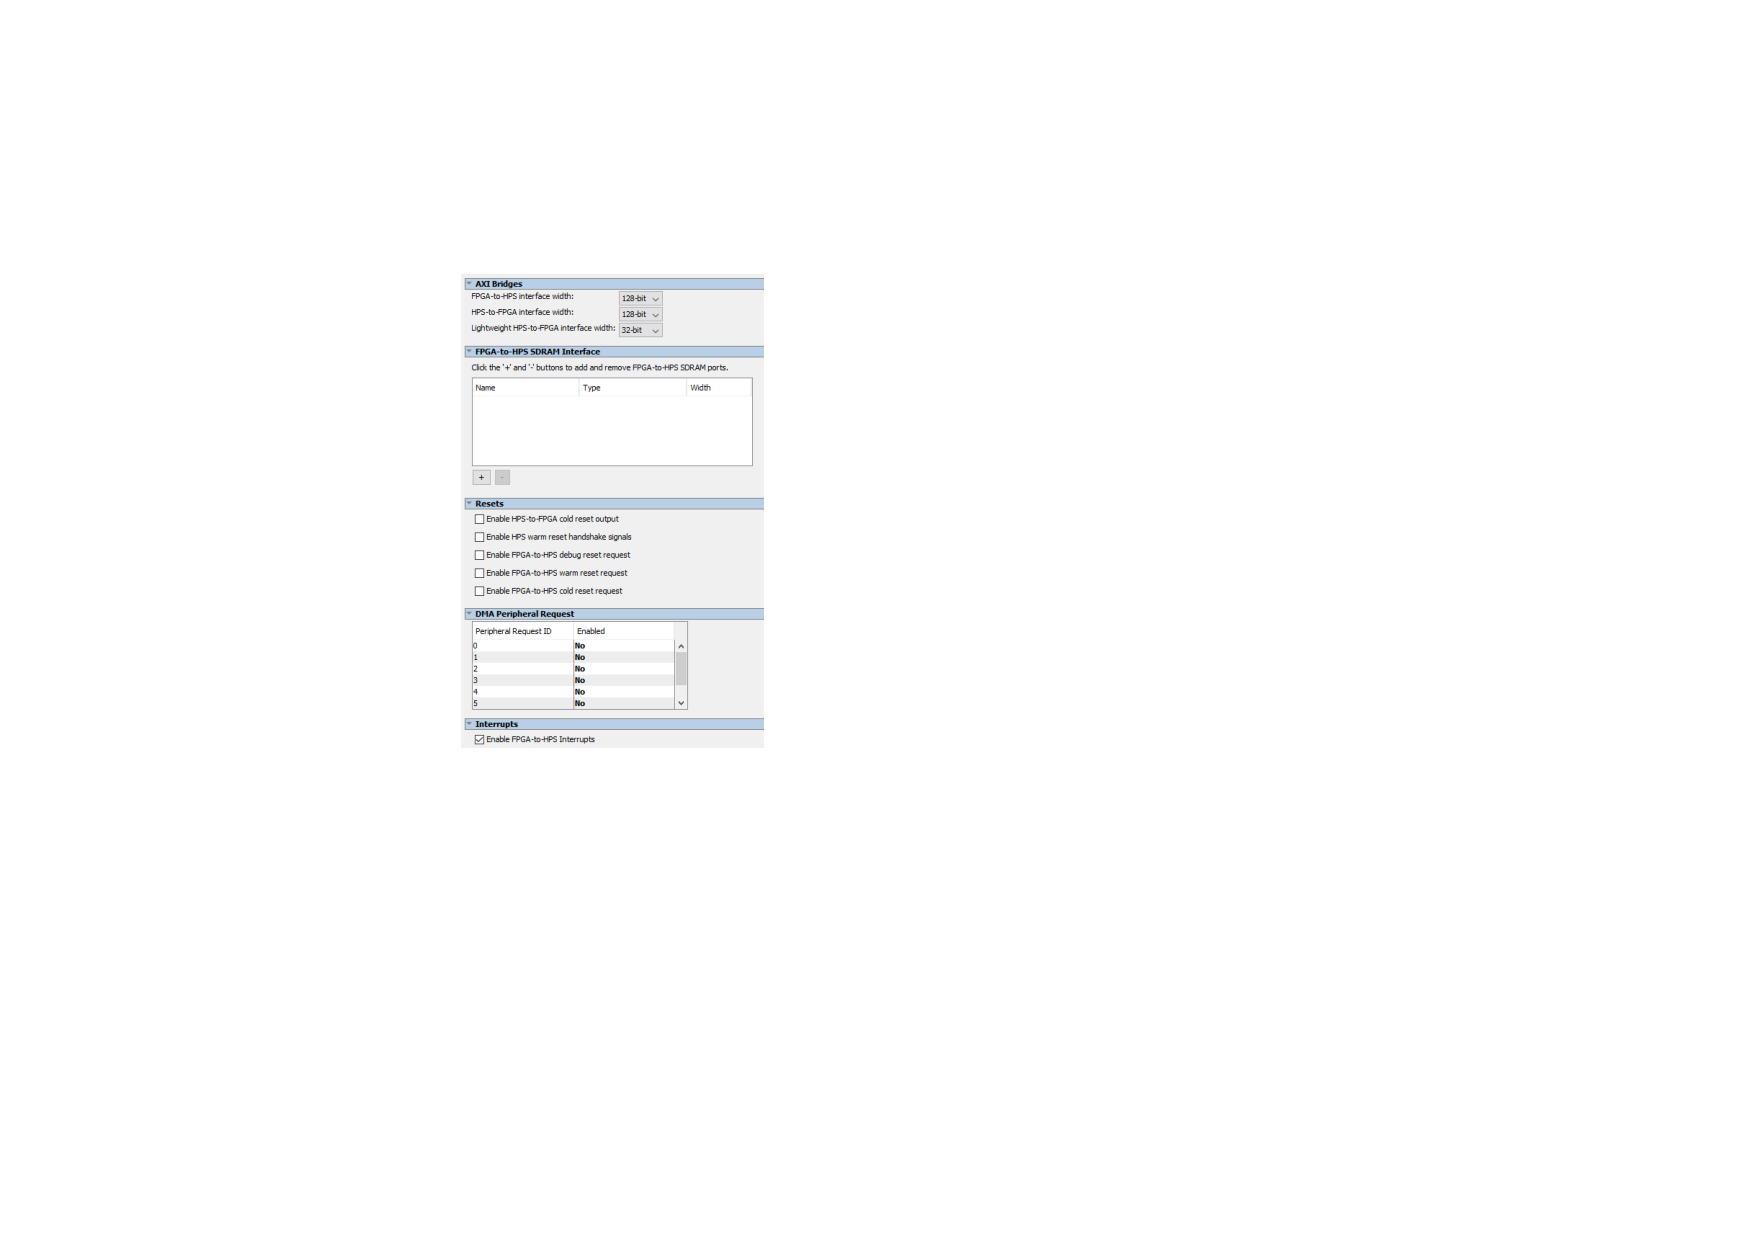
\includegraphics[width=.9\linewidth]{images/hps_fpga_interfaces}
		\caption{\gls{FPGA}-Schnittstellen}
		\label{fig:hps_fpga_interfaces}
	\end{subfigure}%
	\begin{subfigure}{.5\textwidth}
		\centering
		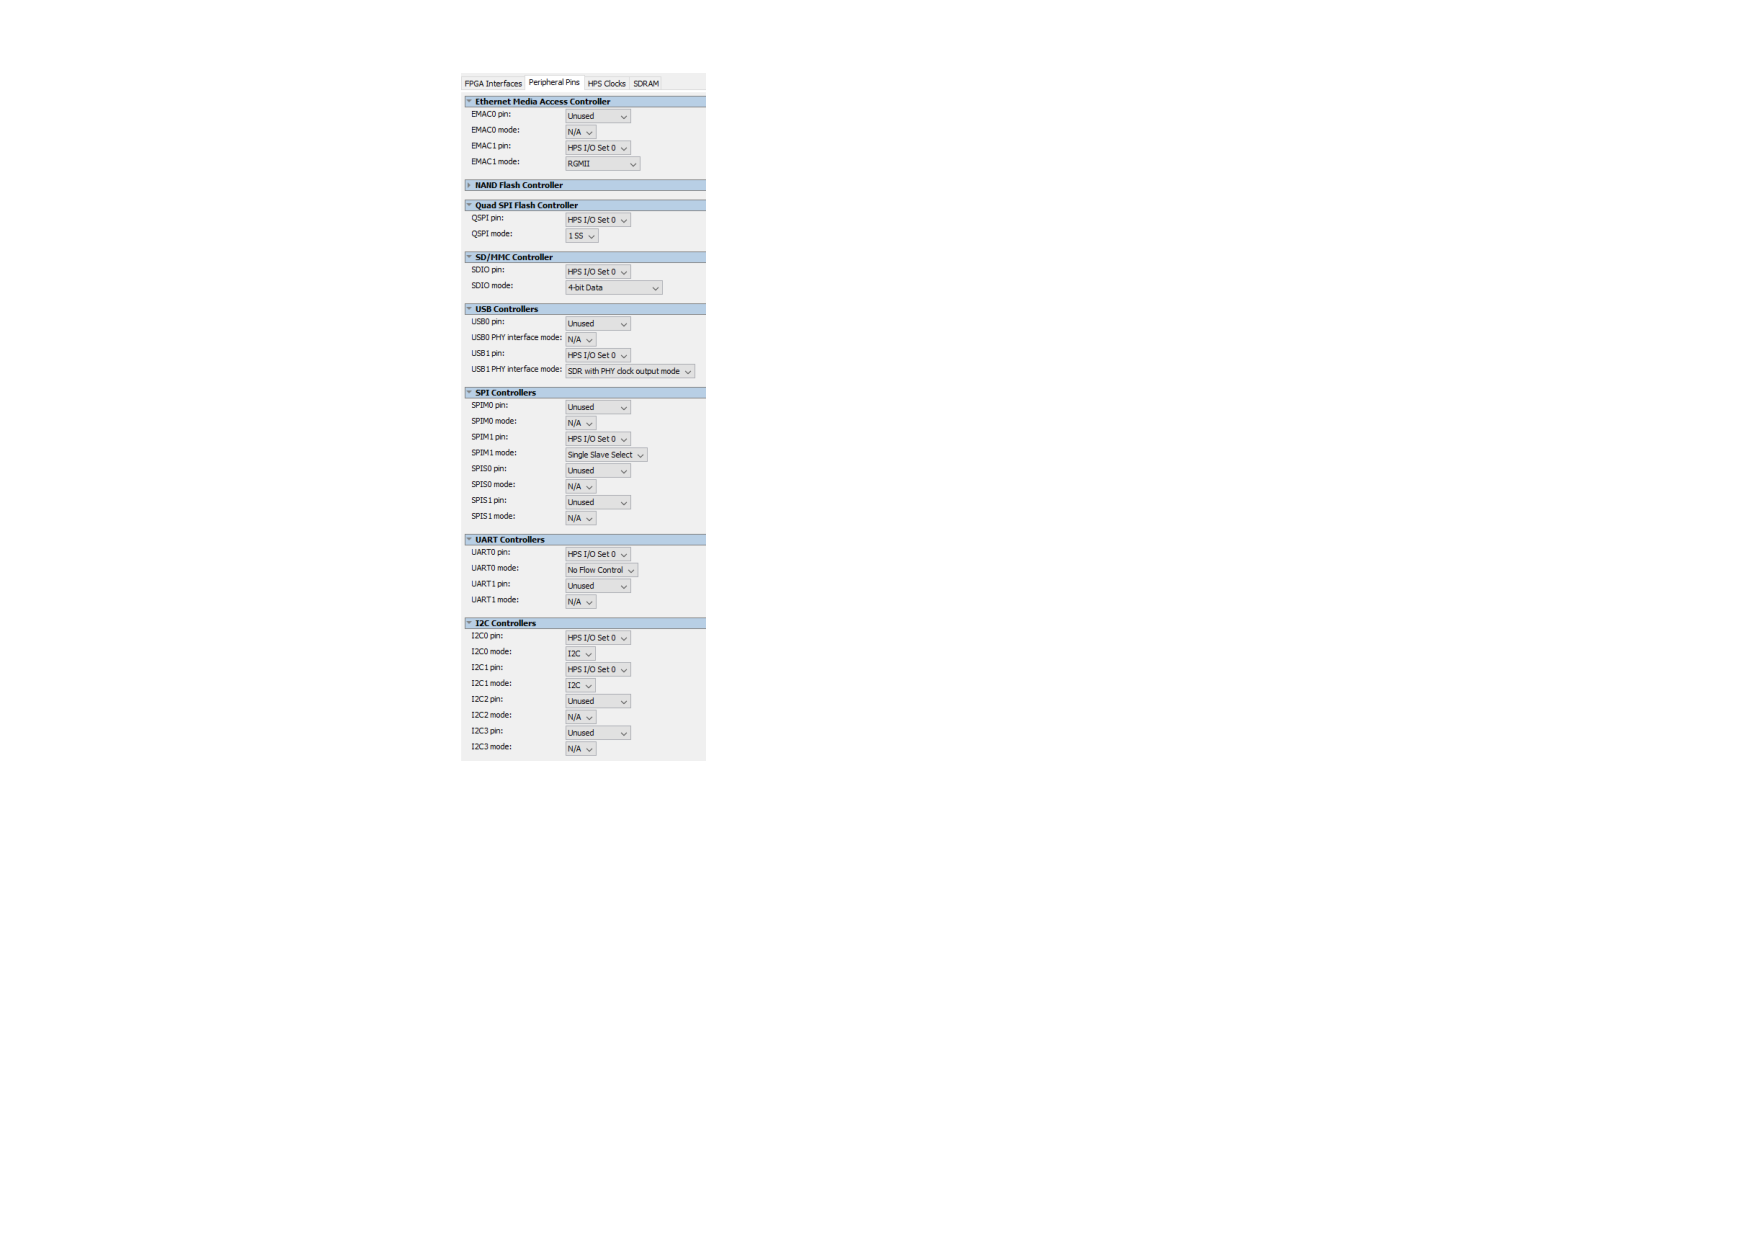
\includegraphics[width=.9\linewidth]{images/hps_periph_pins.pdf}
		\caption{Peripherie-Pins}
		\label{fig:hps_periph_pins}
	\end{subfigure}
	\caption{\gls{HPS}: Konfiguration}
	\label{fig:hps_params}
\end{figure}

Die SDRAM-Konfiguration wird zum bis auf den Memory-Vendor aus einer CERN-Projektdokumentation \cite[6-8]{article:cern_socfpga} übernommen. Die Konfigurationspanels für \gls{PHY}-, \gls{RAM}-, Timing- und Board-Parameter sind in \cref{fig:hps_sdram_params} abgebildet.

\begin{figure}[!htbp]
	\centering
	\begin{subfigure}[b]{0.475\textwidth}
		\centering
		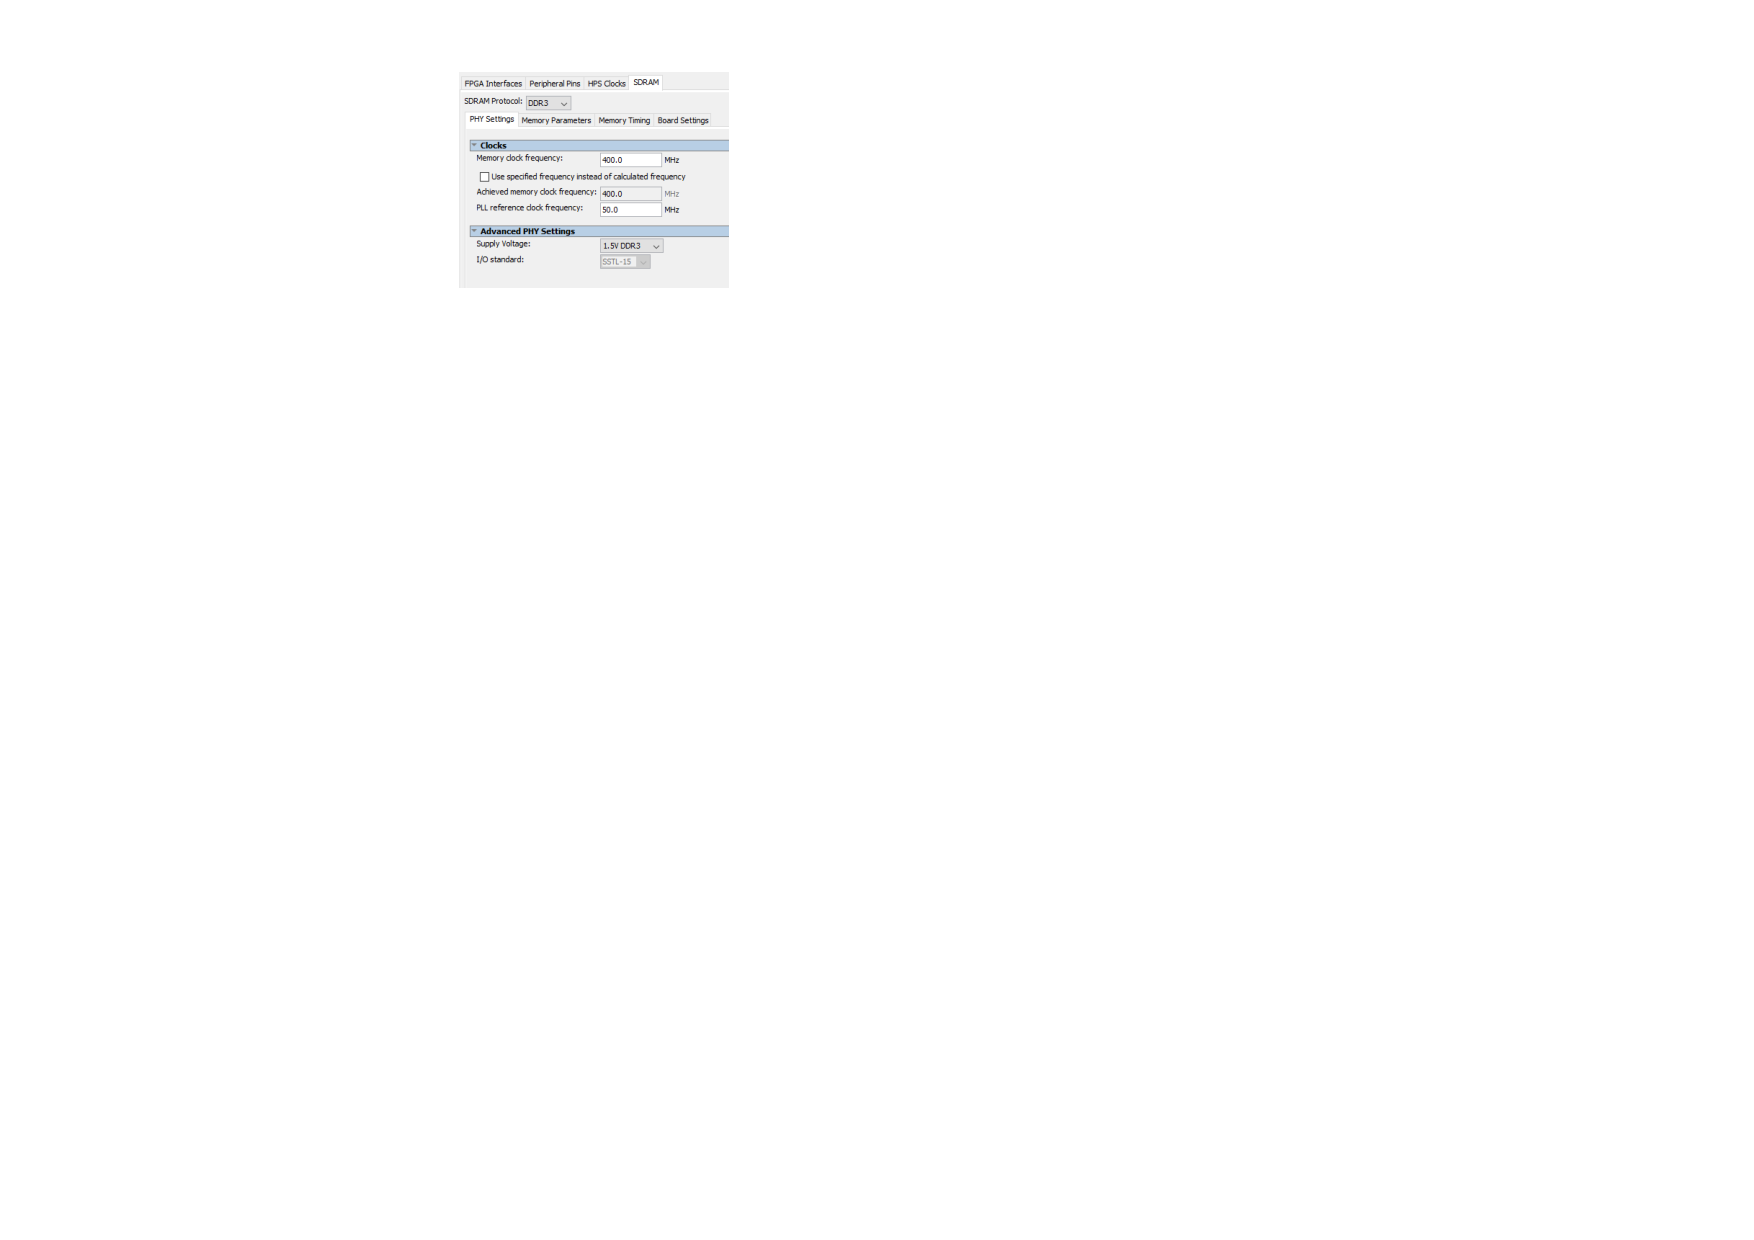
\includegraphics[width=\textwidth]{images/hps_sdram_phy}
	\caption{\gls{PHY}}
		\label{fig:hps_sdram_phy}
	\end{subfigure}
	\hfill
	\begin{subfigure}[b]{0.475\textwidth}  
		\centering 
		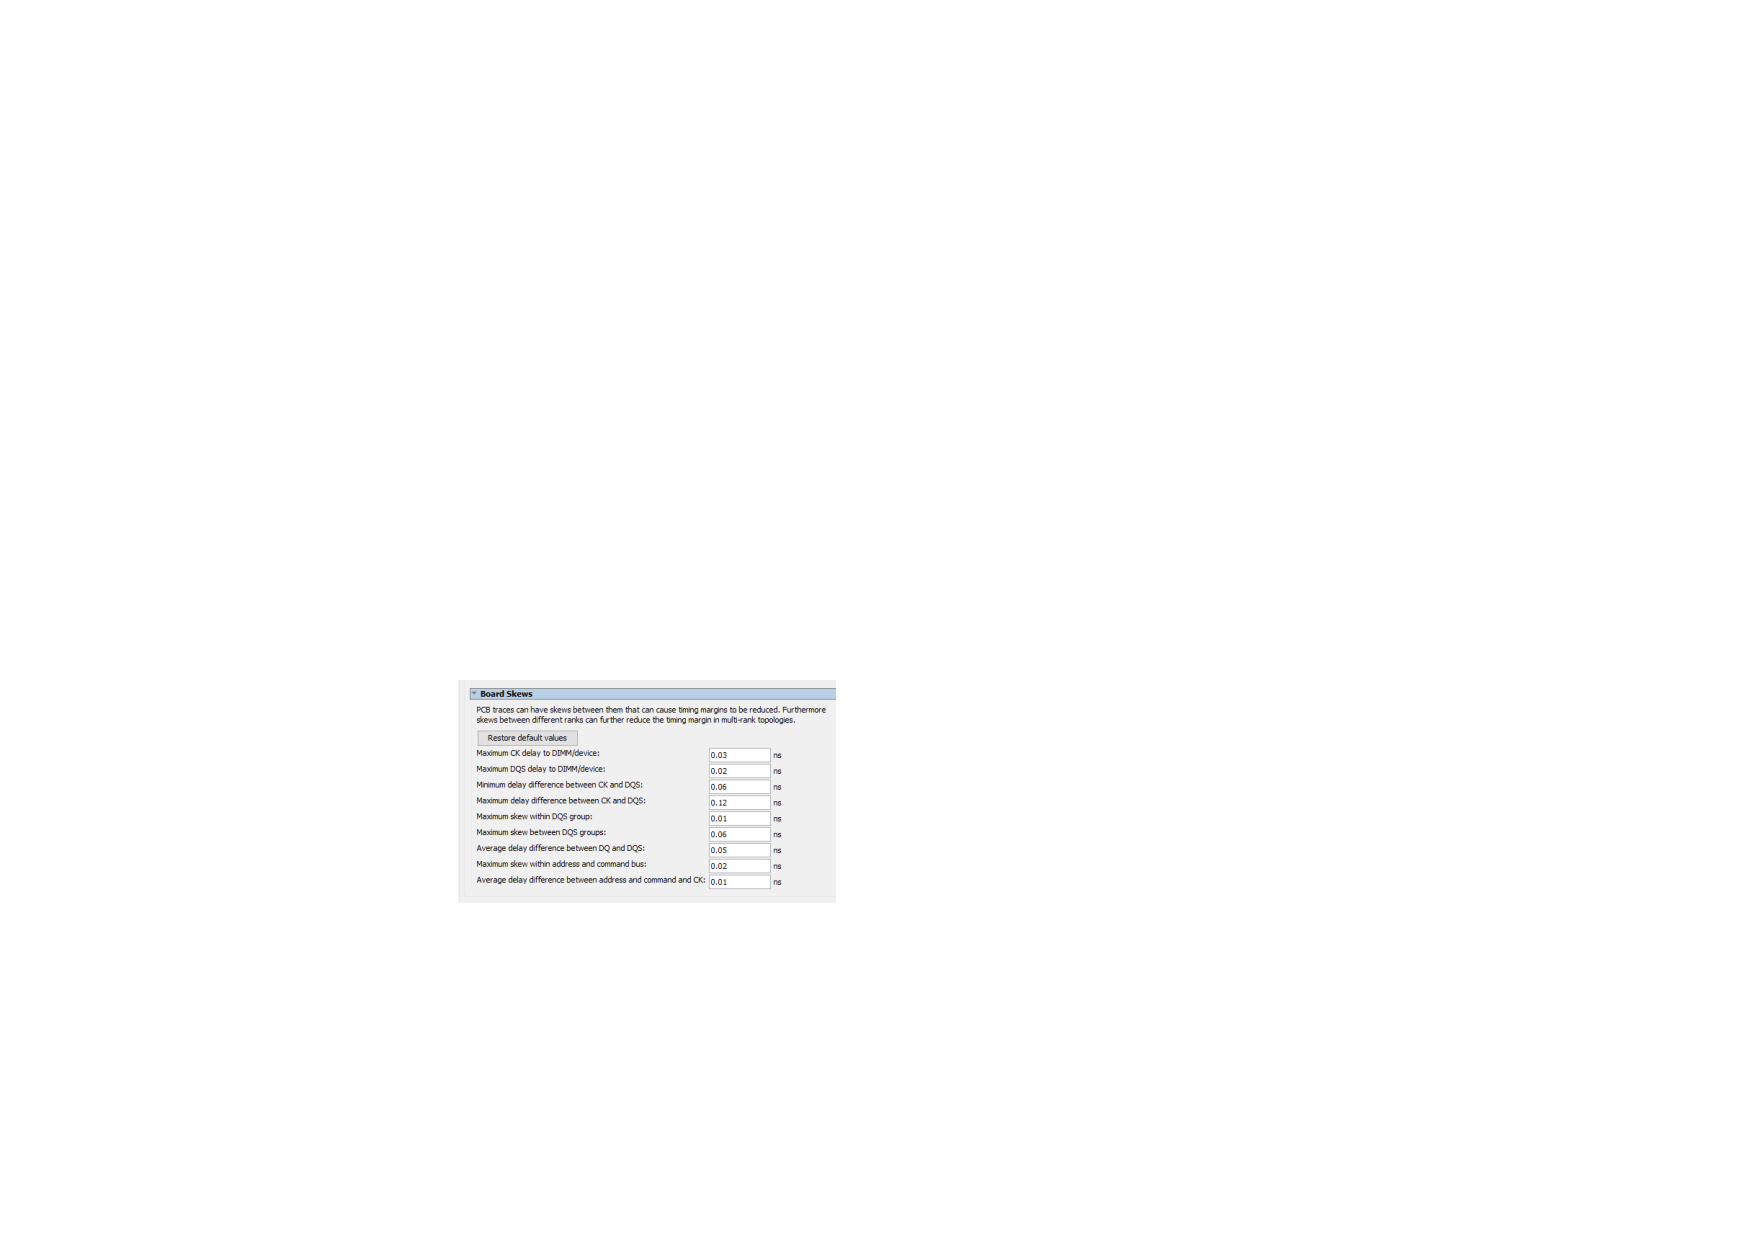
\includegraphics[width=\textwidth]{images/hps_sdram_board_params}
		\caption{Board}
		\label{fig:hps_sdram_board_params}
	\end{subfigure}
	\vskip\baselineskip
	
	\begin{subfigure}[b]{0.475\textwidth}   
		\centering 		
		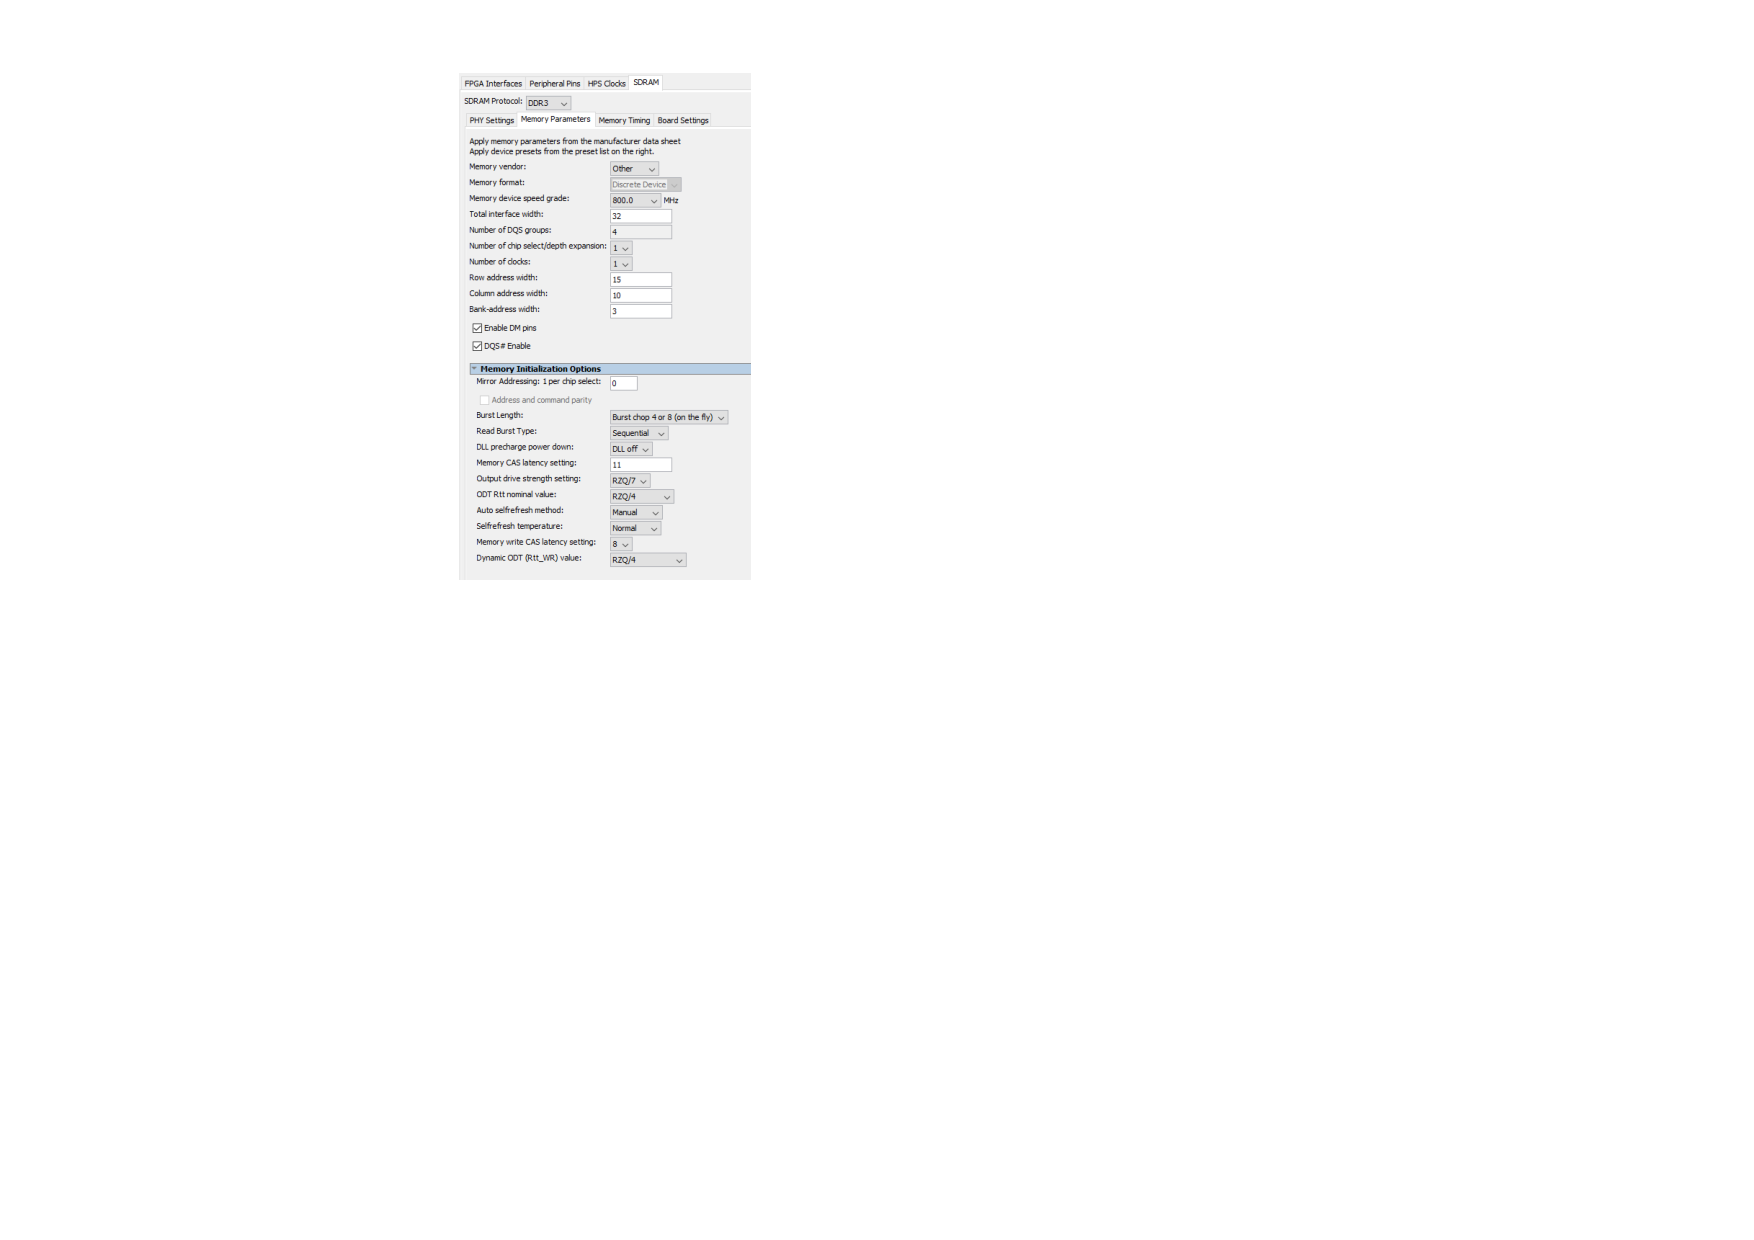
\includegraphics[width=\textwidth]{images/hps_sdram_mem_param}
		\caption{\gls{RAM}}
		\label{fig:hps_sdram_mem_param}
	\end{subfigure}
	\quad
	\begin{subfigure}[b]{0.475\textwidth}   
		\centering 
		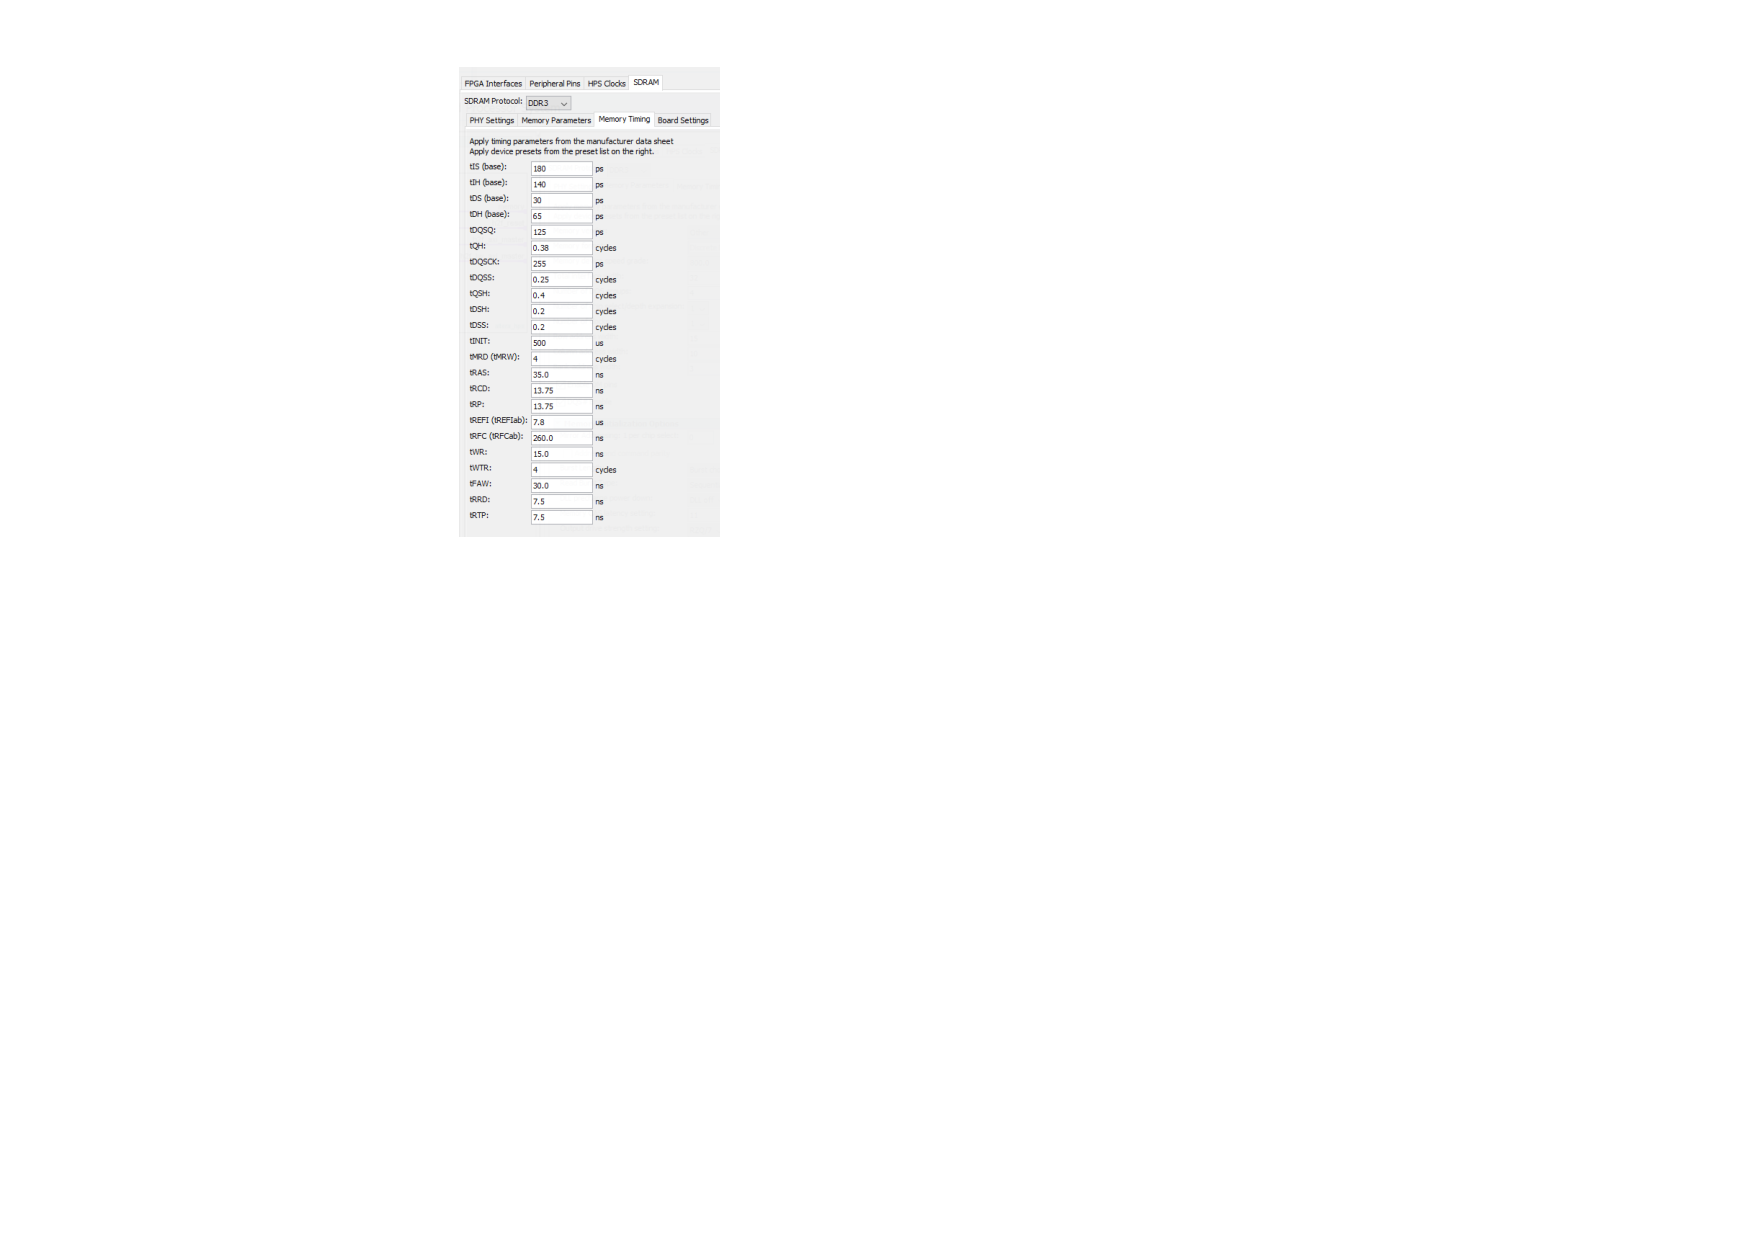
\includegraphics[width=\textwidth]{images/hps_sdram_mem_timings}
		\caption{Timings}
		\label{fig:hps_sdram_mem_timings}
	\end{subfigure}
	\caption{\gls{HPS} SDRAM-Konfiguration}
	\label{fig:hps_sdram_params}
\end{figure}

Nach der Konfiguration des \gls{HPS} und des Arbeitsspeichers muss im Quartus zuerst der \enquote{Analysis \& Synthesis} ausgeführt werden. Danach muss über \textit{Tools}\textrightarrow\textit{TCL Scripts} das \enquote{hps\_sdram\_p0\_assignments.tcl}-Skript ausgeführt werden. Der Skript-Dialog ist in \cref{fig:script_pinassignments} dargestellt.

Dieser Schritt ist notwendig, da vor der Konfiguration keine Timing-Parameter bekannt waren und so keine Pin-Zuweisung für den Arbeitsspeicher vorgenommen werden konnte \cite[46]{article:embedded_systems}. 

\begin{figure}[!htbp]
	\centering
	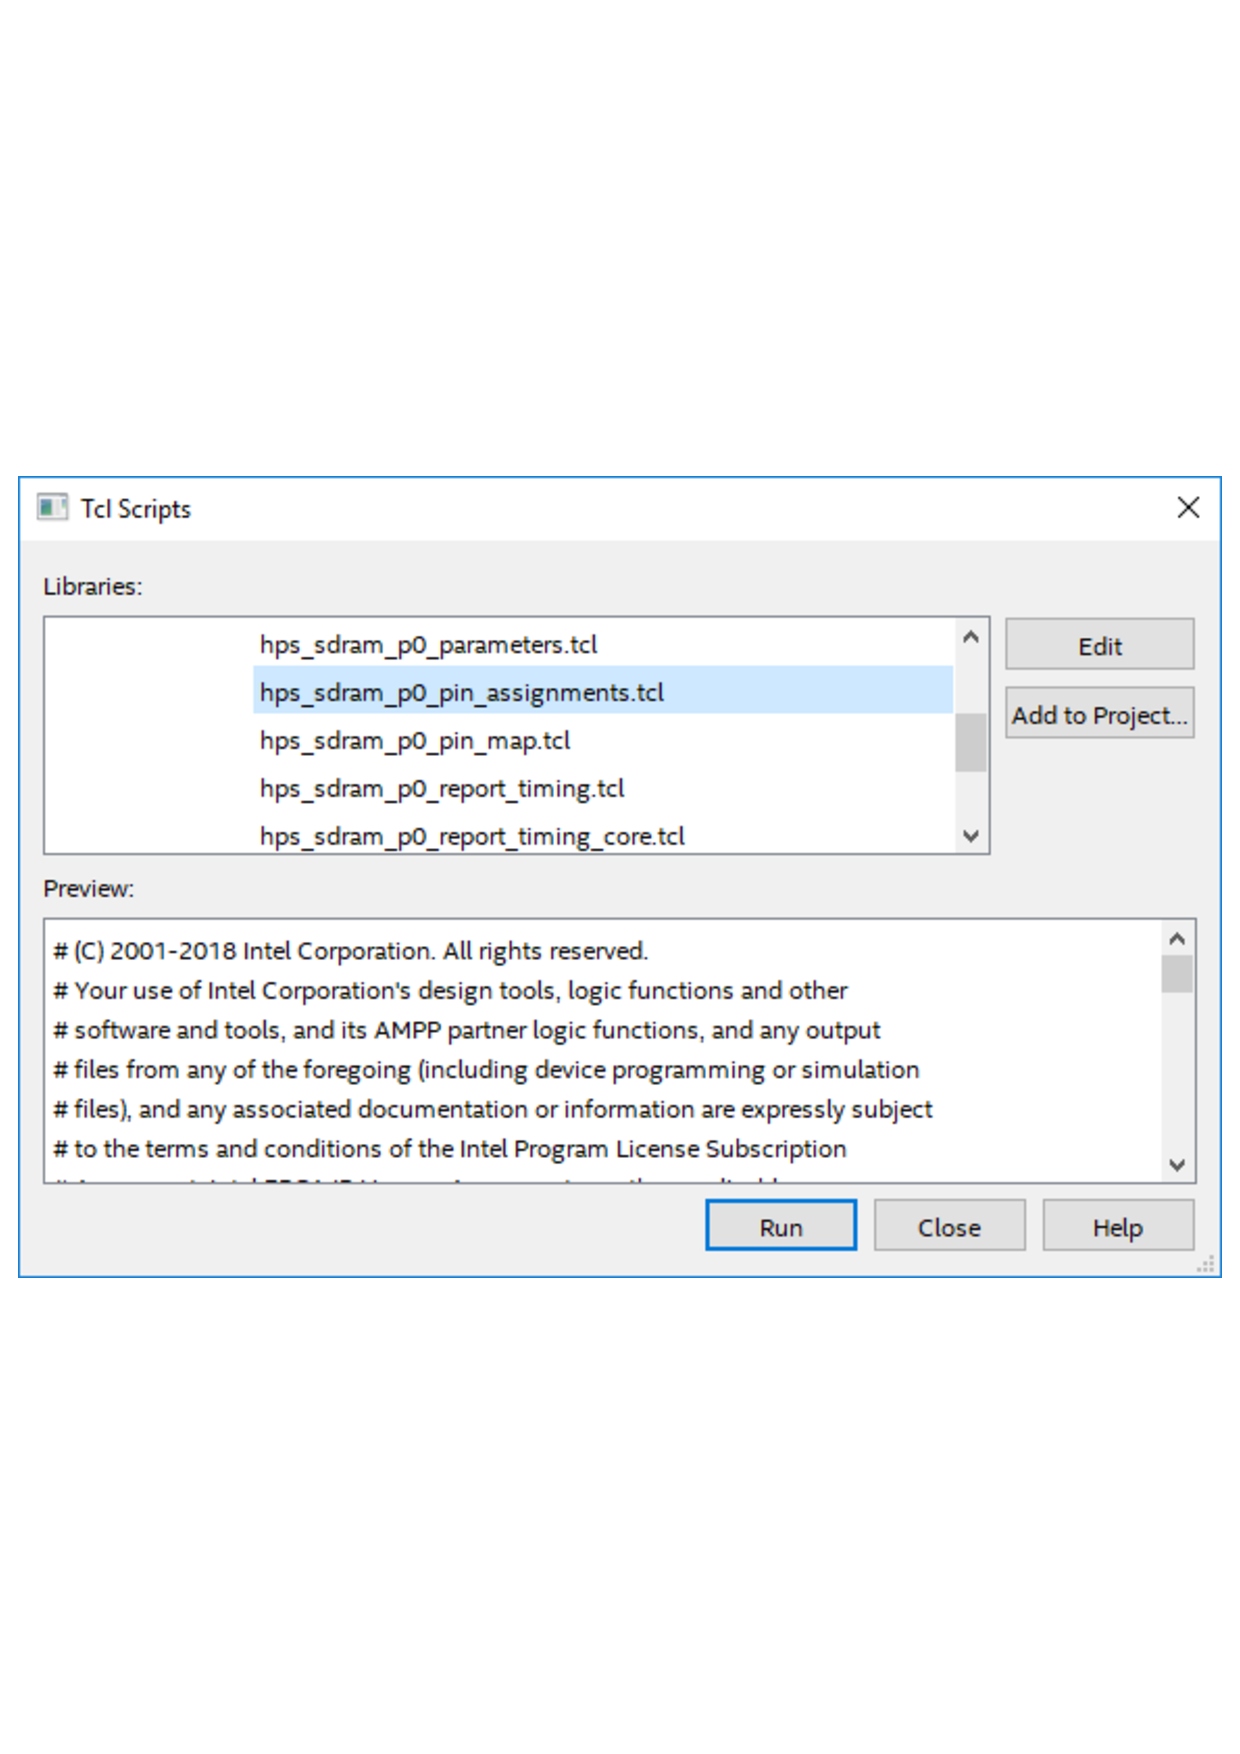
\includegraphics[width=0.61\linewidth]{images/script_pinassignments}
	\caption{Tcl Scripts: hps\_sdram\_p0\_pin\_assignments.tcl}
	\label{fig:script_pinassignments}
\end{figure}

\subsection{System ID}

Ein System ID Peripheral IP-Core wird im Platform Designer hinzugefügt und an die Lightweight \gls{HPS}\textrightarrow{}\gls{FPGA}-Bridge angebunden. Für den einzigen konfigurierbaren Parameter \enquote{\SI{32}{\bit} System-ID} wird der Wert \texttt{0xDEADBEEF} gewählt.

%, wie in \cref{fig:system_id_params} zu sehen ist.
%
%\begin{figure}[!htbp]
%	\centering
%	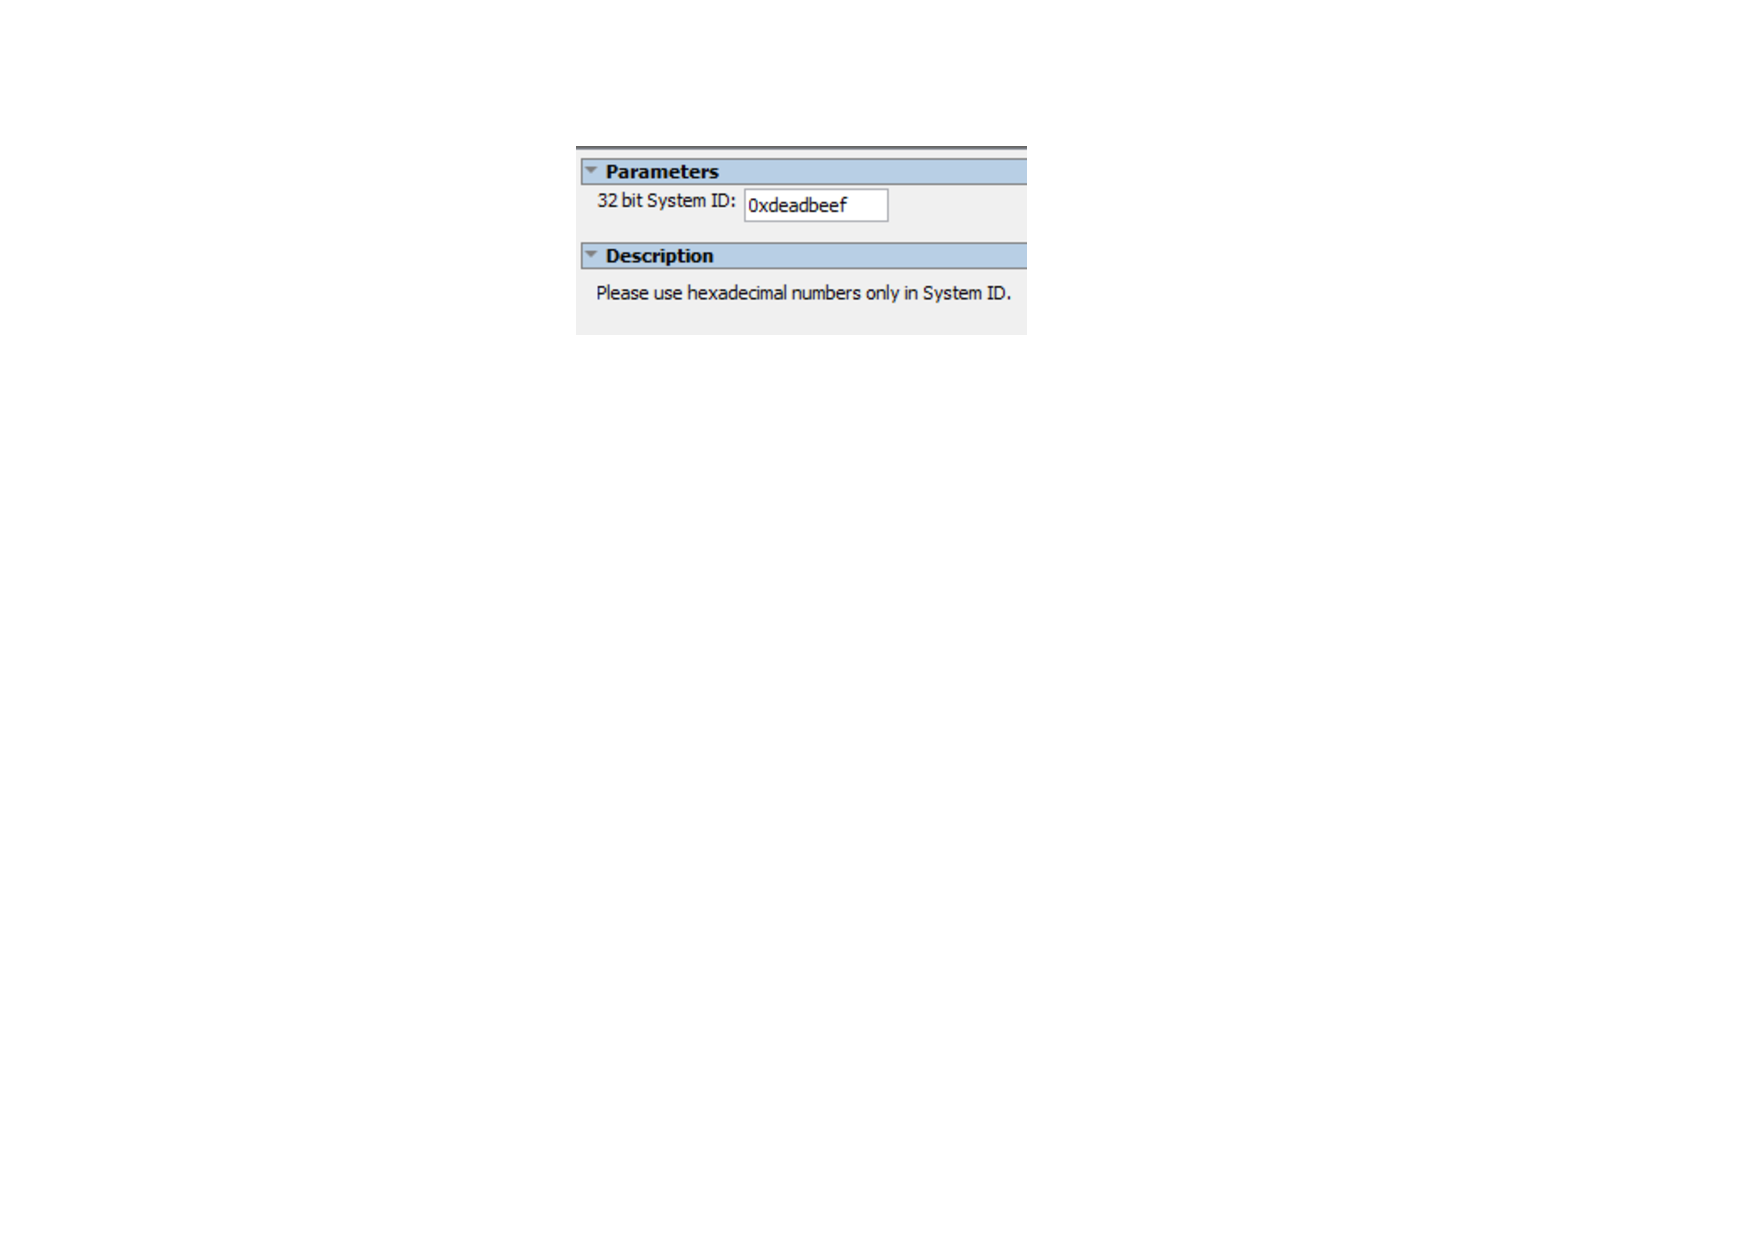
\includegraphics[width=0.4\linewidth]{images/system_id_params}
%	\caption{Parametrisierung des \textit{System ID Peripheral}-IP-Core}
%	\label{fig:system_id_params}
%\end{figure}

\subsection{Adresszuordnung}

Die Adresszuordnung der Plasma-\gls{SoC}-Komponenten wird überarbeitet. Dadurch ergibt sich, wie in \cref{tab:wb_plasma_de1soc_address_map} aufgelistet, eine im Vergleich zur Adresszuordnung in \cref{tab:wb_plasma_zedboard_address_map} und unter Berücksichtigung der neuen Komponenten verbessere Nutzung der Adressbereiche. Über die Wishbone{$\leftrightarrow$}Avalon-\gls{Bridge} angesteuerte Slaves sind mit einem grauen Hintergrund hervorgehoben.

\begin{table}[!htbp]
	\bigskip
	\centering
	\begin{tabular}{| l | r | r |}
		\hline	
		\textbf{Gerät} & \textbf{Startadresse} & \textbf{Adressbereich} \\
		\Xhline{2\arrayrulewidth}		
		\gls{RAM}\textsubscript{0}& \texttt{0x00000000} & \texttt{00001FFF} \\
		\hline		
		IRC\textsubscript{0} & \texttt{0x00005000} & \texttt{0x1F} \\
		\hline		
		UART\textsubscript{0}& \texttt{0x00005100} & \texttt{0x0F} \\
		\hline
		\multirow{4}{*}{Timer\textsubscript{0:3}} & \texttt{0x00005200} & \texttt{0x0F} \\
		& \texttt{0x00005210} & \texttt{0x0F} \\
		& \texttt{0x00005220} & \texttt{0x0F} \\
		& \texttt{0x00005230} & \texttt{0x0F} \\
		\hline
		\multirow{4}{*}{Zähler\textsubscript{0:3}} & \texttt{0x00005300} & \texttt{0x0F} \\
		& \texttt{0x00005310} & \texttt{0x0F} \\
		& \texttt{0x00005320} & \texttt{0x0F} \\
		& \texttt{0x00005330} & \texttt{0x0F} \\
		\hline
		\multirow{4}{*}{GPIO\textsubscript{0:3}}  & \texttt{0x00005400} & \texttt{0x0F} \\
		& \texttt{0x00005410} & \texttt{0x0F} \\
		& \texttt{0x00005420} & \texttt{0x0F} \\
		& \texttt{0x00005430} & \texttt{0x0F} \\
		\hline
		SPI\textsubscript{0} & \texttt{0x00005500} & \texttt{0x0F} \\
		%\hline
		\Xhline{2\arrayrulewidth}
		\rowcolor{gray!30}Wishbone\textrightarrow{}Avalon-\gls{Bridge} & \texttt{0x10000000} & \texttt{0x0FFFFFFF} \\
		\hline
		\rowcolor{gray!20}\gls{RAM}\textsubscript{1} & \texttt{0x10000000} & \texttt{0x03FFFFFF} \\
		\hline
		\rowcolor{gray!20} & \texttt{0x14000070} & \texttt{0x0F} \\
		\rowcolor{gray!20} & \texttt{0x14000060} & \texttt{0x0F} \\
		\rowcolor{gray!20} & \texttt{0x14000050} & \texttt{0x0F} \\
		\rowcolor{gray!20} & \texttt{0x14000040} & \texttt{0x0F} \\
		\rowcolor{gray!20} & \texttt{0x14000030} & \texttt{0x0F} \\
		\rowcolor{gray!20} \multirow{-6}{*}{HEX\textsubscript{0:5}} & \texttt{0x14000020} & \texttt{0x0F} \\
		\hline
		\rowcolor{gray!20} Schalter\textsubscript{0} & \texttt{0x14000010} & \texttt{0x0F} \\
		\hline
		\rowcolor{gray!20} Taster\textsubscript{0} & \texttt{0x14000000} & \texttt{0x0F} \\
		\hline
	\end{tabular}
	
	\caption[Plasma-SoC Adresszuordnung]{Plasma-SoC Adresszuordnung. Grau markierte Komponenten sind an die Wishbone\textrightarrow{}Avalon-\gls{Bridge} angebunden }
	\label{tab:wb_plasma_de1soc_address_map}
\end{table}

\subsection{Zusammenfassung}

Das Gesamtsystem besteht nun aus einem \gls{SoC}-\gls{FPGA} mit einem Plasma-\gls{SoC} im \gls{FPGA}-Bereich. 
Auf alle Geräte und Speicher des Plasma-\gls{SoC} kann vom \gls{HPS} aus zugegriffen werden, da nun, wie in \cref{fig:complete_system} zu sehen ist, alle Komponenten über einen Bus mit dem \gls{HPS} verbunden sind.

\begin{figure}[!htbp]
	\centering
	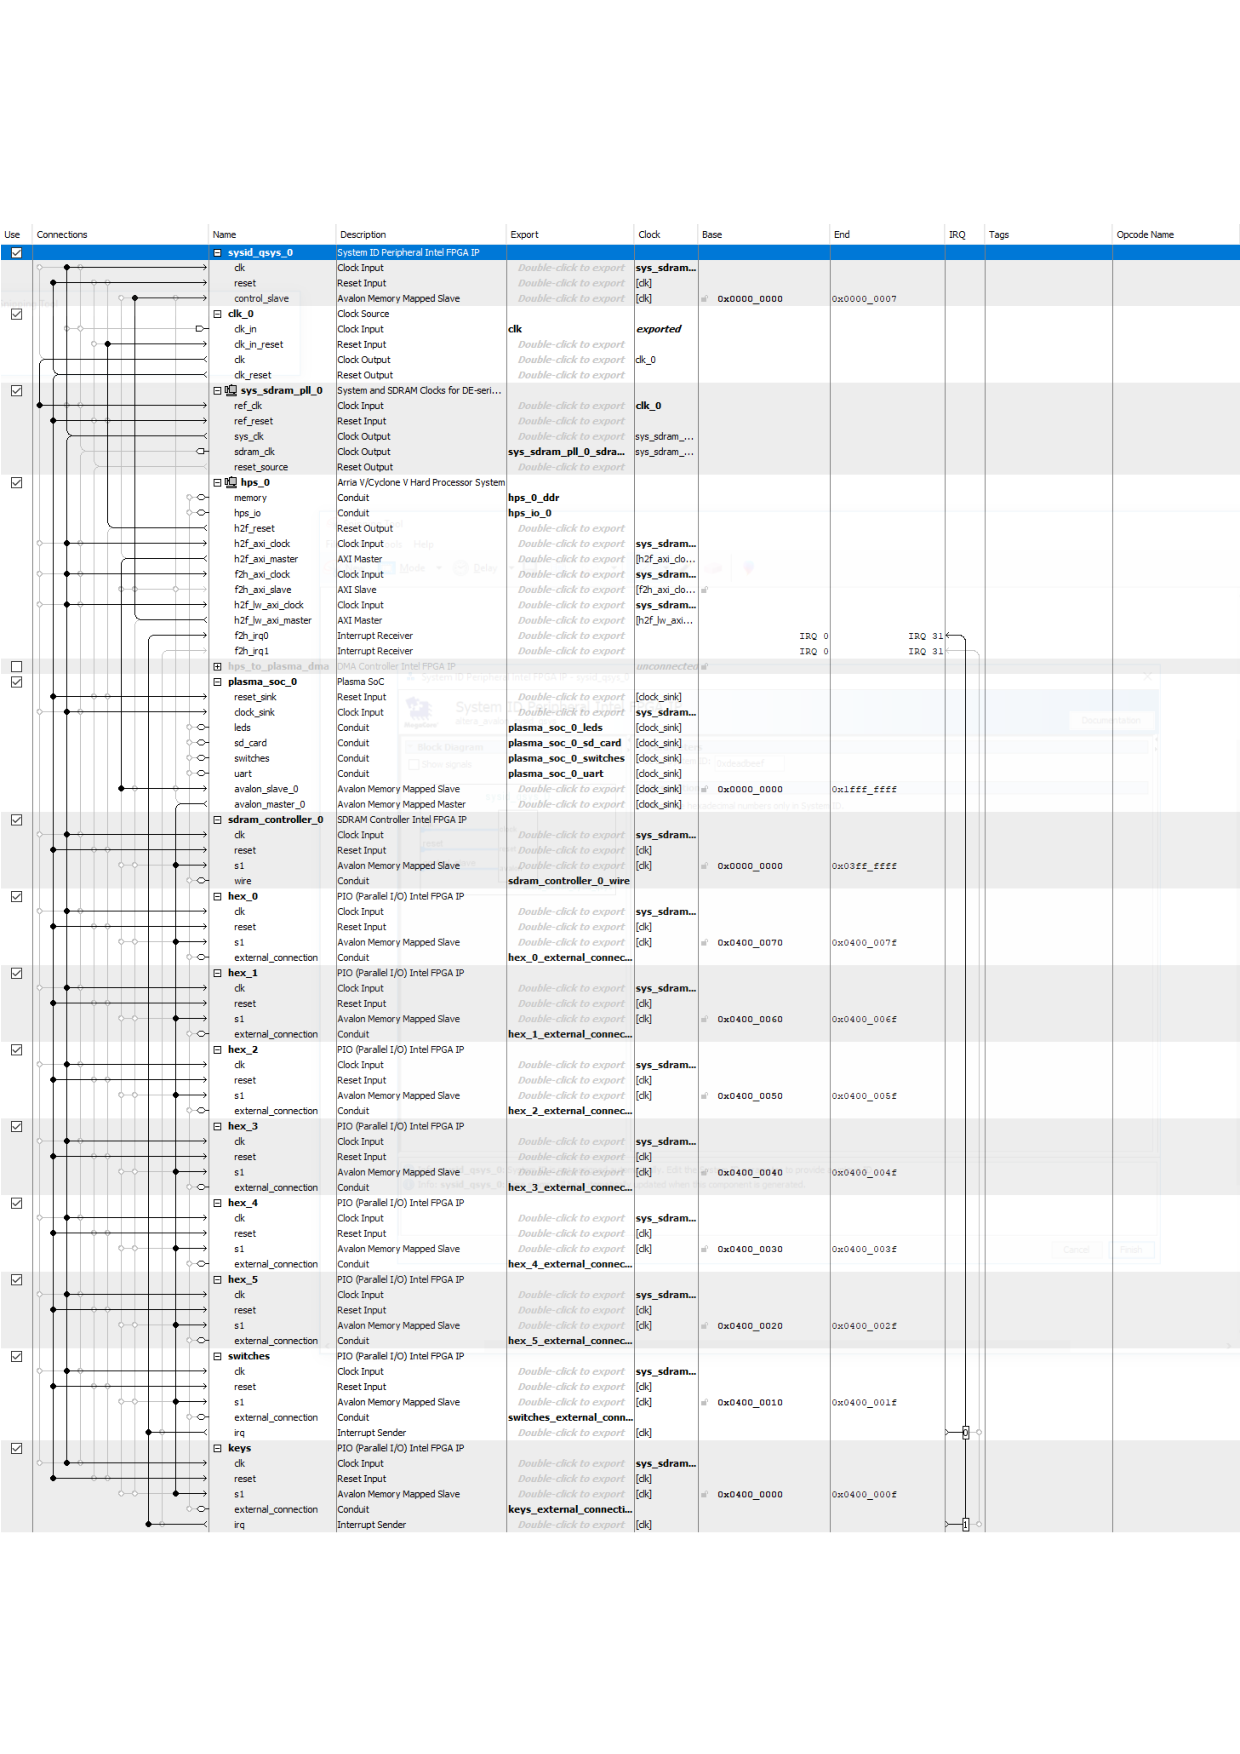
\includegraphics[width=1\linewidth]{images/complete_system}
	\caption{Das Gesamtsystem im Platform Designer}
	\label{fig:complete_system}
\end{figure}


\section{Unterstützende Software}
\label{sec:impl_extend_tools_for_de1_soc}

Zur Initialisierung des internen Arbeitsspeichers muss, wie bereits im \cref{sec:impl_port_hw_to_de1_soc} erwähnt, eine \gls{MIF}-Datei verwendet werden. Um den Speicher mit einer \gls{ELF}-Datei zu initialisieren, wird das \texttt{convert.py}-Skript um einen dem MIF-Format \cite{manual:mif_help} entsprechenden \gls{MIF}-Generator erweitert.

%Diese Datei hat eine im \cref{lst:mif_format} angegebene Struktur. 

%\begin{code}	
%	\begin{minted}[breaklines, autogobble]{text}
%	-- Speichertiefe (DEPTH) und -breite (WIDTH) sind Pflichtfelder	
%	-- DEPTH und WIDTH werden als Dezimalzahlen angegeben
%	DEPTH = 32; -- DEPTH ist die Anzahl der Adressen
%	WIDTH = 14; -- WIDTH ist die Datenwortbreite
%	
%	-- Adress- und Datenbasis sind Pflichtfelder
%	-- Erlaubte Werte: BIN, DEC, HEX, OCT, oder UNS; 
%	-- Standardwert: HEX	
%	ADDRESS_RADIX = HEX; 
%	DATA_RADIX = HEX; 
%	
%	-- Hier werden Adress und Wertpaare angegeben. 
%	-- Adressen können sowohl als Einzeladressen als auch Adressbereiche angegeben werden.
%	CONTENT 
%	BEGIN 
%	[0..F] :   3FFF;  -- Adressbereich: Alle Adressen von 0 bis F = 3FFF
%	6      :   F;     -- Einzeladresse: Adresse 6 = F
%	8      :   F E 5; -- Adressbereich mit einer festgelegten Startadresse
%	                  -- Addr[8] = F, Addr[9] = E, Addr[A] = 5
%	END; 
%	
%	\end{minted}
%	
%	\caption{Struktur des Memory Initialization File \cite{manual:mif_help}}
%	\label{lst:mif_format}
%\end{code}

Ein längere Zeit bestehendes Problem des in \cref{sec:arch_plasma_soc_zedboard} beschriebenen Systems ist das scheinbar von der Programmgröße abhängige Laufzeitverhalten. Durch eine simulationsbasierte Überprüfung des zeitlichen Verlaufs der am Wishbone-Bus anliegenden Adressen und Daten wird festgestellt, dass Variablen in den \texttt{.sdata} und \texttt{.sbss}-Sektionen überschrieben werden. Die Vermutung, dass die Linker-Konfiguration fehlerhaft ist, wird durch einen Vergleich zwischen dem standard-Linkerskript für \gls{MIPS}-\RN{1}-Prozessoren und der eigenen Linker-Konfiguration bestätigt. 

Auffällig sind die nicht übereinstimmenden Positionen der Global Pointer (\texttt{\_gp}) und die Byte-Ausrichtungen. Die eigene Linker-Konfiguration wird so korrigiert, dass der Global Pointer wie im Standard-Linkerskript zwischen den \texttt{.data} und \texttt{.sdata}-Sektionen liegt und an einer \SI{16}{\byte}-Grenze ausgerichtet ist. Nach dieser Korrektur werden die \texttt{.sdata} und \texttt{.sbss}-Sektionen zu keinem Zeitpunkt überschrieben und eine korrekte Ausführung der Anwendungen ist gewährleistet.

%Das voreingestellte Linkerskript lässt sich durch Aufruf des Linkers mit dem \texttt{-verbose}-Schalter ausgeben: \texttt{mips-linux-gnu-ld -verbose}. Die auf das Wesentliche reduzierte Ausgabe ist im \cref{lst:linkerscript_default} zu sehen. 
%
%\begin{code}	
%	\begin{minted}[breaklines, autogobble, highlightlines=7]{text}
%	...
%	.data :
%	{
%		...
%	}
%	...
%	HIDDEN (_gp = ALIGN (16) + 0x7ff0);
%	...
%	.sdata :
%	{
%	...
%	}
%	...
%	.sbss :
%	{
%	...
%	}
%	
%	\end{minted}
%	
%	\caption{MIPS-\RN{1} - Linkerskript (Voreinstellung)}
%	\label{lst:linkerscript_default}
%\end{code}
%
%Zum Vergleich ist im \cref{lst:linkerscript_faulty} die auf das Wesentliche reduzierte eigene Linker-Konfiguration angegeben.
%Auffällig ist, dass die Positionen des Global Pointer (\texttt{\_gp}) sowie die Byte-Ausrichtung nicht übereinstimmen. Die eigene Linker-Konfiguration (siehe \cref{lst:linkerscript_faulty}) wird so korrigiert, dass der Global Pointer wie in \cref{lst:linkerscript_default} zwischen den \texttt{.data} und \texttt{.sdata}-Sektionen liegt und an einer \SI{16}{\byte}-Grenze ausgerichtet ist. Nach dieser Korrektur werden die \texttt{.sdata} und \texttt{.sbss}-Sektionen zu keinem Zeitpunkt überschrieben und eine korrekte Ausführung der Anwendungen ist gewährleistet.
%
%\begin{code}
%	
%	\begin{minted}[breaklines, autogobble, highlightlines=11]{text}
%	...
%	.data :
%	{ 
%	...
%	}
%	...	
%	.sdata :
%	{
%	... 
%	}		
%	__gp = .;		
%	.sbss : 
%	{
%	...
%	}
%	...
%	\end{minted}
%	
%	\caption{MIPS-\RN{1} - Linkerskript (Fehlerhaft)}
%	\label{lst:linkerscript_faulty}
%\end{code}


\section{Portierung der Plasma-Firmware und der Beispielanwendung}
\label{sec:impl_port_plasma_sw_to_de1_soc}
Die Portierung der Firmware erfolgt in Form einer neuen Systemdefinitionsdatei mit einer neuen Adresszuordnung und anderen Komponenten. Die bestehende Definition wird in die Datei \texttt{platform/plasma\_soc.zedboard.h} ausgelagert, und die neue in der Datei \texttt{platform/plasma\_soc.de1\_soc.h} erstellt. Die CMake Build-Skripte werden um neue Einträge erweitert, welche die zwei verschiedenen Systemkonfigurationen repräsentieren. Dabei wird ein Präprozessor-Makro definiert, welcher in der Datei \texttt{plasma\_soc.h} ausgewertet wird und dadurch die passende Systemdefinition einbezogen wird.
Die Headerverzeichnisse der Firmware werden ebenfalls umbenannt, um Kollisionen mit den Linux-Headerverzeichnissen zu vermeiden: \textit{dev} und \textit{sys} werden jeweils mit dem Präfix \enquote{k} versehen. 

Aus der Beispielanwendung werden die Funktionen für die \gls{UART}-Ein- und Ausgabe sowie die Displayausgabe entfernt. 
Stattdessen erfolgt die Anzeige der seit dem Systemstart vergangenen Zeit über die auf dem Board vorhandenen 7-Segment Anzeigen. Dafür wird eine Funktion entwickelt, welche für Ganzzahlen im Bereich von \texttt{0x0...0xF} für Common-Anode 7-Segment-Anzeigen geeignete Codes zurückgibt.

Die LED-Lauflichtfunktion wird erweitert, sodass die Richtung und Muster konfigurierbar sind. Das LED-Muster ist im externen SDRAM über die Adresse \texttt{0x800} und die Richtung über der Adresse \texttt{0x804} ansprechbar.

\section{Einrichtung eines Linux-Betriebssystems}
\label{sec:impl_setup_linuxfor_de1_soc}

In diesem Abschnitt wird in mehreren Schritten vom Devicetree über Bootloader und Kernel bis hin zur Entwicklung eines Treibers ein individuell eingerichtetes Linux-Betriebssystem erstellt. Sehr hilfreich für das Verständnis ist die Embedded-Linux Anleitung von RocketBoards.org \cite{website:embedded_linux_beginners_guide}.
\subsection{Devicetree}
\label{sec:impl_devicetree}
Damit im Betrieb unter Linux die Hardware richtig erkannt wird und auch eigene Treiber geladen werden können, muss eine Devicetree-Definition erstellt werden. 

Zwar ist es möglich, mit der Altera SoC EDS Entwicklungsumgebung eine Device-Tree-Datei zu generieren, jedoch ist das Ergebnis nicht zufriedenstellend. Bis auf die Plasma-\gls{SoC}- und SysID-Einträge fehlen alle weiteren im Platform Designer definierten Komponenten. Außerdem führen Kompatibilitätsprobleme mit verschiedenen Kernel-Versionen zur Fehlfunktion der Treiber und/oder Absturz des Systems. 

Aus diesem Grund wird gemäß Spezifikation Devicetree v0.2 \cite{manual:devicetree_specification} eine für das Plasma-\gls{SoC} und das DE1-SoC-Board geeignete Devicetree-Datei \texttt{socfpga\_cyclone5\_de1\_soc.dts} entworfen. Mit dem C-Präprozessor werden die Definitionen aus den Originaldateien \texttt{socfpga.dtsi} und \texttt{socfpga\_cyclone5.dtsi} miteinander verknüpft \cite[Version~4.9.78-ltsi, \texttt{arch/arm/boot/dts/}]{website:linux_socfpga_repository}. 


Nachfolgend werden die wichtigsten Fragmente beschrieben. 

%Das \texttt{sopc2dts}-Programm erwartet eine \texttt{sopcinfo} Datei, welche bei der Generierung der HDL-Dateien im Platform Designer entsteht. 
%
%\begin{code}	
%	\begin{minted}[breaklines, autogobble]{text}
%	sopc2dts --input ${sopcinfo} \
%	--output dts/plasma_soc.dts \
%	--type dts \
%	--board dts/soc_system_board_info.xml \
%	--board dts/hps_clock_info.xml \
%	--bridge-removal all
%	\end{minted}
%	
%	\caption{Ausschnitt aus der generierten DTS-Datei}
%	\label{lst:sopc2dts}
%\end{code}

%Die mit den Altera-Tools aus der \texttt{sopcinfo}-Datei generierte Devicetree-Defintion ist nicht zufriedenstellend. Bis auf die Plasma-\gls{SoC}- und SysID-Einträge fehlen alle weiteren im Platform Designer angebundenen Komponenten. Außerdem sind die Gerätebeschreibungen nicht mit allen Kernel-Versionen kompatibel, was zur Folge hat, dass die Treiber unter Umständen nicht korrekt funktioneren oder das System nicht startet. 

%\begin{code}	
%	\begin{minted}[breaklines, autogobble]{text}
%	... 
%	hps_0_bridges: bridge@0xc0000000 {
%		compatible = "altr,bridge-18.0", "simple-bus";
%		reg = < 0xC0000000 0x20000000 0xFF200000 0x00200000 >;
%		reg-names = "axi_h2f", "axi_h2f_lw";
%		#address-cells = < 2 >;
%		#size-cells = < 1 >;
%		ranges = < 0x00000000 0x00000000 0xC0000000 0x20000000 0x00000001 0x00000000 0xFF200000 0x00000008 >;
%		
%		plasma_soc_0: unknown@0x000000000 {
%			compatible = "unknown,unknown-1.0";
%			reg = < 0x00000000 0x00000000 0x20000000 >;
%		}; //end unknown@0x000000000 (plasma_soc_0)
%		
%		sysid_qsys_0: sysid@0x100000000 {
%			compatible = "ALTR,sysid-18.0", "ALTR,sysid-1.0", "altr,sysid-1.0";
%			reg = < 0x00000001 0x00000000 0x00000008 >;
%			id = < 3735928559 >;	/* embeddedsw.dts.params.id type NUMBER */
%			timestamp = < 1536706156 >;	/* embeddedsw.dts.params.timestamp type NUMBER */
%		}; //end sysid@0x100000000 (sysid_qsys_0)
%	}; //end bridge@0xc0000000 (hps_0_bridges)
%	...
%	\end{minted}
%	
%	\caption{Ausschnitt aus der generierten DTS-Datei}
%	\label{lst:generated_dts}
%\end{code}

%Darum wird gemäß Devicetree Spezifikation \cite{manual:devicetree_specification} eine für das Plasma-SoC auf dem DE1-SoC-Board geeignete Devicetree-Datei \texttt{socfpga\_cyclone5\_de1\_soc.dts} entworfen. Über einen include-Mechanismus werden die Definitionen aus den Originaldateien \texttt{socfpga.dtsi} und \texttt{socfpga\_cyclone5.dtsi} vererbt \cite[Version~4.9.78-ltsi, \texttt{arch/arm/boot/dts/}]{website:linux_socfpga_repository}. Nachfolgend werden die wichtigsten Fragmente beschrieben. 

%Zunächst werden die Kernel-Bootargumente angegeben:
%\begin{code}
%	\begin{minted}[breaklines, autogobble]{text}
%		chosen {
%			bootargs = "earlyprintk debug console=ttyS0,115200 root=/dev/mmcblk0p2 rw rootwait mem=768M";
%		};.
%	\end{minted}
%	\caption{Devicetree: Kernel-Bootargumente}
%	\label{lst:custom_dts_bootarg_def}
%\end{code}

Die Definition des Arbeitsspeichers wird um Einträge für den internen und externen (siehe \cref{sec:external_sdram}) \gls{RAM} des Plasma-SoC erweitert:
\begin{code}
	\begin{minted}[breaklines, autogobble]{text}
	memory@0 {
		name = "memory";
		device_type = "memory";
		reg =   <0x00000000 0x40000000>, /* 1GB DDR3 */
			<0xC0000000 0x00002000>, /* 8KB Plasma RAM0 */
			<0xD0000000 0x00010000>; /* 64MB Plasma RAM1 */
	};
	\end{minted}
	\caption{Devicetree: Arbeitsspeicherdefinition}
	\label{lst:custom_dts_memory_defs}
\end{code}

Die HPS-Bridge-Definition wird vervollständigt. Das Wichtigste hier ist die Adress-Translation über den \texttt{ranges}-Ausdruck: Die Basisadresse \texttt{0xFF200000} (lightweight HPS‐to‐FPGA bridge \cite[21]{article:embedded_systems}) mit dem Adressbereich \texttt{0x8} wird auf \texttt{0,0}, die Basisadresse \texttt{0xC0000000} (HPS‐to‐FPGA Bridge \cite[22]{article:embedded_systems}) mit dem Adressbereich \texttt{0x5510} wird auf \texttt{1,0}, und die Basisadresse \texttt{0xD4000000} mit dem Adressbereich \texttt{0x80} wird auf \texttt{2,0} abgebildet. Eingehende Basisadressen und Adressbereiche sind im \cref{lst:custom_dts_bridge_ranges} orange markiert, und die Zielbereiche entsprechend grün.

\begin{code}
	\begin{minted}[breaklines, autogobble, escapeinside=||]{text}
	hps_0_bridges: bridge@c0000000 {
		compatible = "altr,bridge-1.0", "simple-bus";
		reg = < 0xC0000000 0x20000000 0xFF200000 0x00200000 >;
		reg-names = "axi_h2f", "axi_h2f_lw";
		#address-cells = < 2 >;
		#size-cells = < 1 >;
		ranges = <|\colorbox{green}{0 0}| |\colorbox{orange}{0xFF200000 0x00000008}| >,
			 <|\colorbox{green}{1 0}| |\colorbox{orange}{0xC0000000 0x00005510}| >,
			 <|\colorbox{green}{2 0}| |\colorbox{orange}{0xD4000000 0x00000080}| >;
		 ...
	\end{minted}
	
	\caption{Devicetree: Adresstranslation in der HPS-Bridge}
	\label{lst:custom_dts_bridge_ranges}
\end{code}

Dem aus der Basisadresse \texttt{0xFF200000} transliertem Adressbereich \texttt{0,0} wird im \cref{lst:custom_dts_sysid} die Beschreibung des SysID-IP-Core zugeordnet. 
\begin{code}
	\begin{minted}[breaklines, autogobble]{text}
	hps_0_bridges: bridge@c0000000 {
	...
		sysid_qsys_0: sysid@0,0 {
			compatible = "ALTR,sysid-13.1", "ALTR,sysid-1.0", "altr,sysid-1.0";
			reg = <0 0 0x00000008>;
			id = < 3735928559 >;
			timestamp = < 1536342590 >;
		}; 
	...
	\end{minted}
	
	\caption{Devicetree: SysID-Definition}
	\label{lst:custom_dts_sysid}
\end{code}

Weiter werden im \cref{lst:custom_dts_plsoc_devices} die Beschreibungen für die im Plasma-SoC am Wishbone-Bus angebundenen Timer, Zähler und \glspl{GPIO} definiert.
Diese sind dem aus der Basisadresse \texttt{0xC0000000} transliertem Adressbereich \texttt{1,0} zugeordnet.
\begin{code}
	\begin{minted}[breaklines, autogobble, escapeinside=||]{text}
	hps_0_bridges: bridge@c0000000 {		 
	...
		timer@1,5200 {
			compatible = "plsoc,timer";
			reg = <1 0x5200 0x10>;
		};
		
	... weitere 3 timer
		
		counter@1,5300 {
			compatible = |\colorbox{orange}{"plsoc,counter"}|;
			reg = <1 0x5300 0x10>;
		};
		
	... weitere 3 Zähler
		
		gpio@1,5400 {
			compatible = "plsoc,gpio";
			reg = <1 0x5400 0x10>;
		};
		
	... weitere 3 GPIOs
		
		spi@1,5500 {
			compatible = "plsoc,spi";
			reg = <1 0x5500 0x10>;
		};
	...
	\end{minted}
	
	\caption{Devicetree: Komponenten im Plasma-SoC}
	\label{lst:custom_dts_plsoc_devices}
\end{code}

Zum Schluss werden die über die Avalon-Wishbone-Bridge angebundenen sechs 7-Segment-Anzeigen, der Schalterblock und der Tasterblock beschrieben:
\begin{code}
	\begin{minted}[breaklines, autogobble]{text}
	hps_0_bridges: bridge@c0000000 {		 
	...
		hex0: gpio@2,70 {
			compatible = "altr,pio-15.0", "altr,pio-1.0";
			reg = <2 0x70 0x00000010>;
			altr,gpio-bank-width = <7>;		
			#gpio-cells = <1>;
			gpio-controller;			
		};
	
	... weitere fünf 7-Segment-Anzeigen
	
		switches: gpio@2,10 {
			compatible = "altr,pio-15.0", "altr,pio-1.0";
			reg = <2 0x10 0x00000010>;							
			altr,gpio-bank-width = <10>;
			#gpio-cells = <1>;
			gpio-controller;			
		};
		
		keys: gpio@2,0 {
			compatible = "altr,pio-15.0", "altr,pio-1.0";
			reg = <2 0x00 0x00000010>;
			altr,gpio-bank-width = <4>;	
			#gpio-cells = <1>;						
			gpio-controller;				
		};
	...
	\end{minted}
	
	\caption{Devicetree: Komponenten am Avalon-Bus}
	\label{lst:custom_dts_avalon_periph}
\end{code}

Im letzten Schritt wird der Devicetree in ein Binärformat kompiliert, damit er vom Kernel verwendet werden kann. Dafür wird der Devicetree-Compiler \texttt{dtc} benötigt. 

Schwierigkeiten bereitet die Zusammenführung von drei Devicetree-Dateien mit dem C-Präprozessor zu einer, da der Devicetree-Compiler die zusammengeführte Datei nicht akzeptiert. Eine Untersuchung ergibt, dass der Devicetree-Compiler mehrere aufeinanderfolgende DTS-Header \enquote{/dts-v1/;} nicht verarbeiten kann. Diese Wiederholungen entstehen durch die Vorverarbeitung mit dem C-Präprozessor. Ein Update des Devicetree-Compilers behebt das Problem auch nicht. 

Als Workaround wird ein Shell-Skript entwickelt, welches die Devicetree-Dateien mit dem C-Präprozessor zusammenführt und mit einem regulären Ausdruck alle außer dem ersten Vorkommen von \enquote{/dts-v1/;} entfernt. Diese Nachbearbeitung führt dazu, dass die Devicetree-Dateien erfolgreich kompiliert werden.

\subsection{Bootloader}
\label{sec:impl_bootloader}

Für das DE1-SoC werden aus den Platform-Designer Daten der Preloader und der Bootloader \enquote{U-Boot} generiert. Hierzu wird das Programm \texttt{bsp-editor} aus dem SoC-EDS-Paket aufgerufen und ein neues \gls{BSP} erstellt. Im sich öffnendem Dialog, welcher in \cref{fig:bsp_editor_handoff} dargestellt ist, wird in das Feld \enquote{Preloader settings directory} der Pfad zum \textit{hps\_isw\_handoff/de1\_soc\_hps\_0}-Ordner im Quartus-Projektverzeichnis eingetragen. In diesem Verzeichnis befinden sich durch den Platform-Designer generierte C-Headerdateien mit Parametern zur Konfiguration der Taktgeneratoren, \glspl{PLL}, \glspl{RAM}, \glspl{IO} und Pin-Multiplexer. 

\begin{figure}[!htbp]
	\centering
	\begin{subfigure}{.5\textwidth}
		\centering
		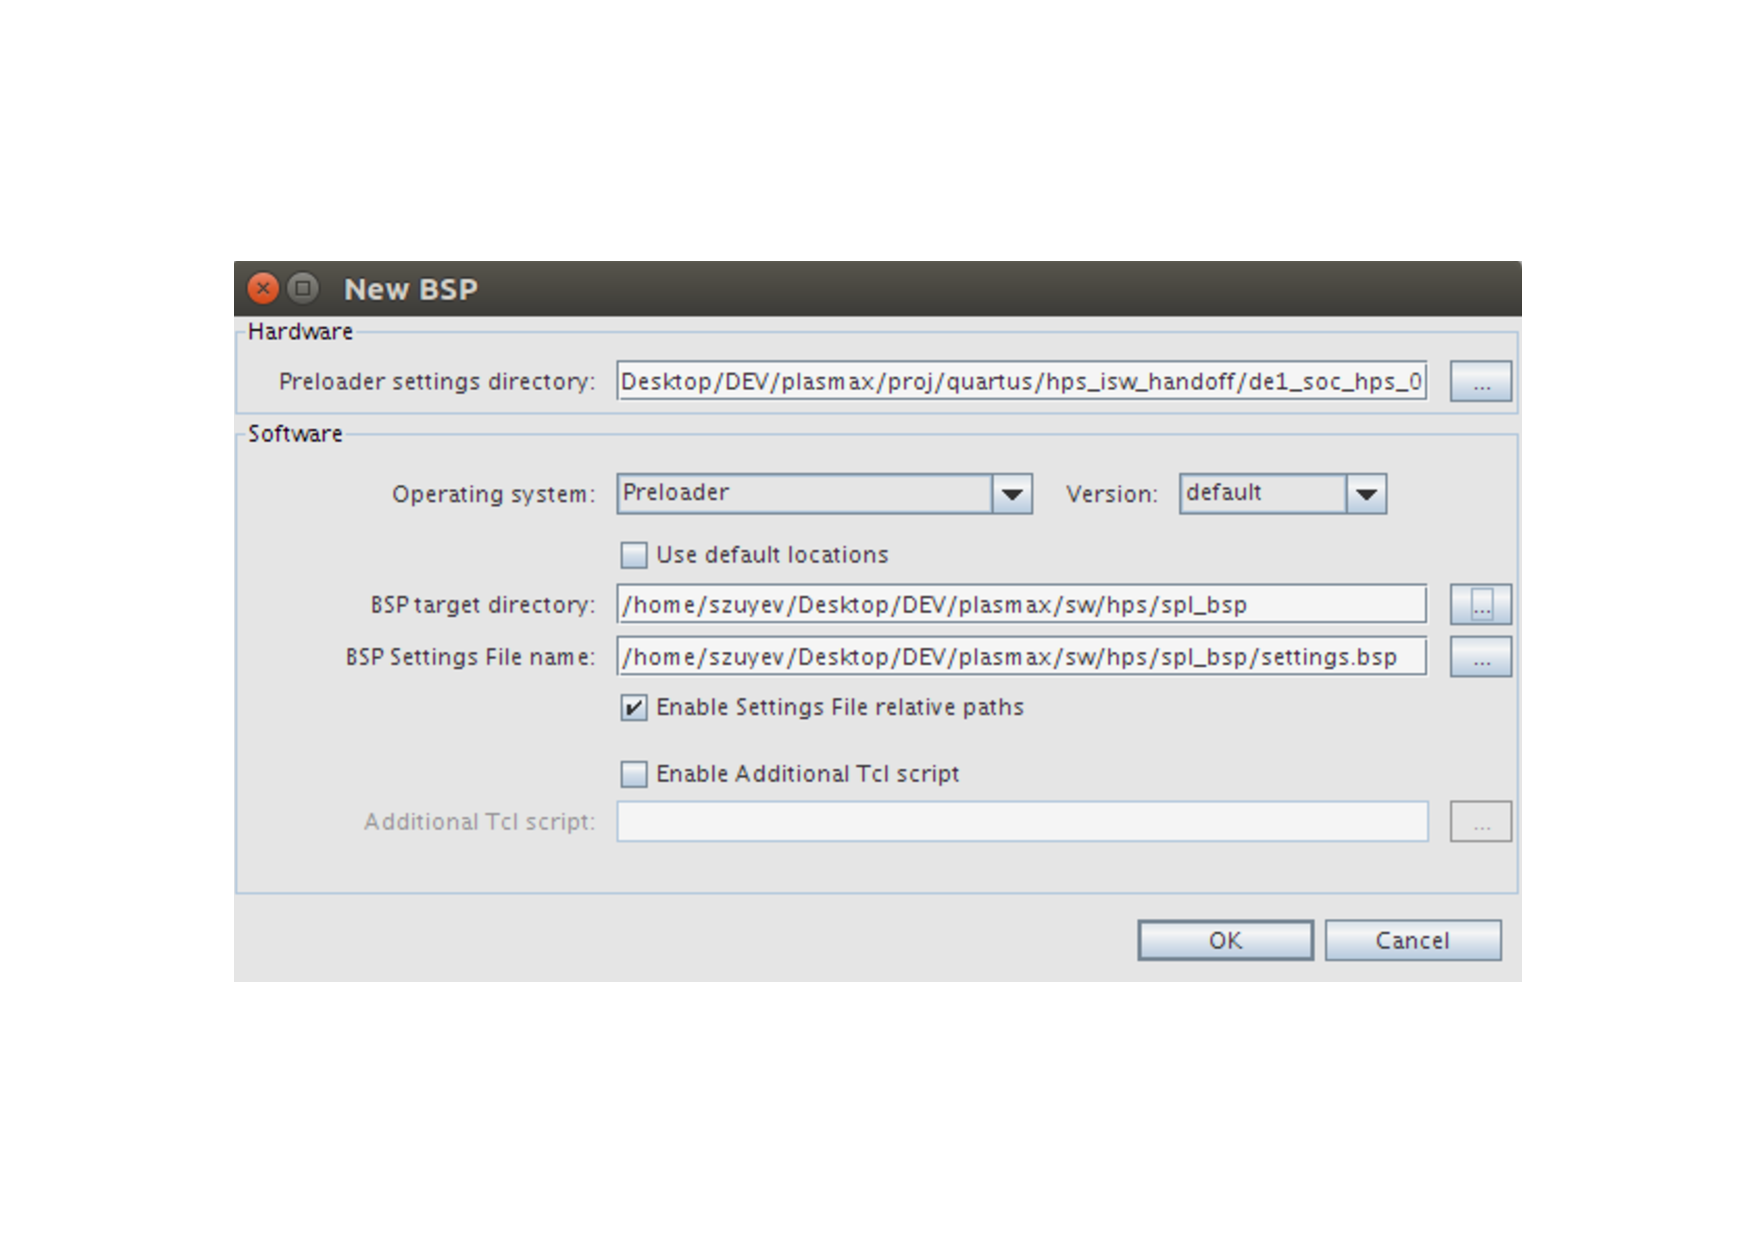
\includegraphics[width=0.9\linewidth]{images/bsp_editor_handoff}
		\caption{Konfiguration eines neuen BSP}
		\label{fig:bsp_editor_handoff}
	\end{subfigure}%
	\begin{subfigure}{.5\textwidth}
		\centering
		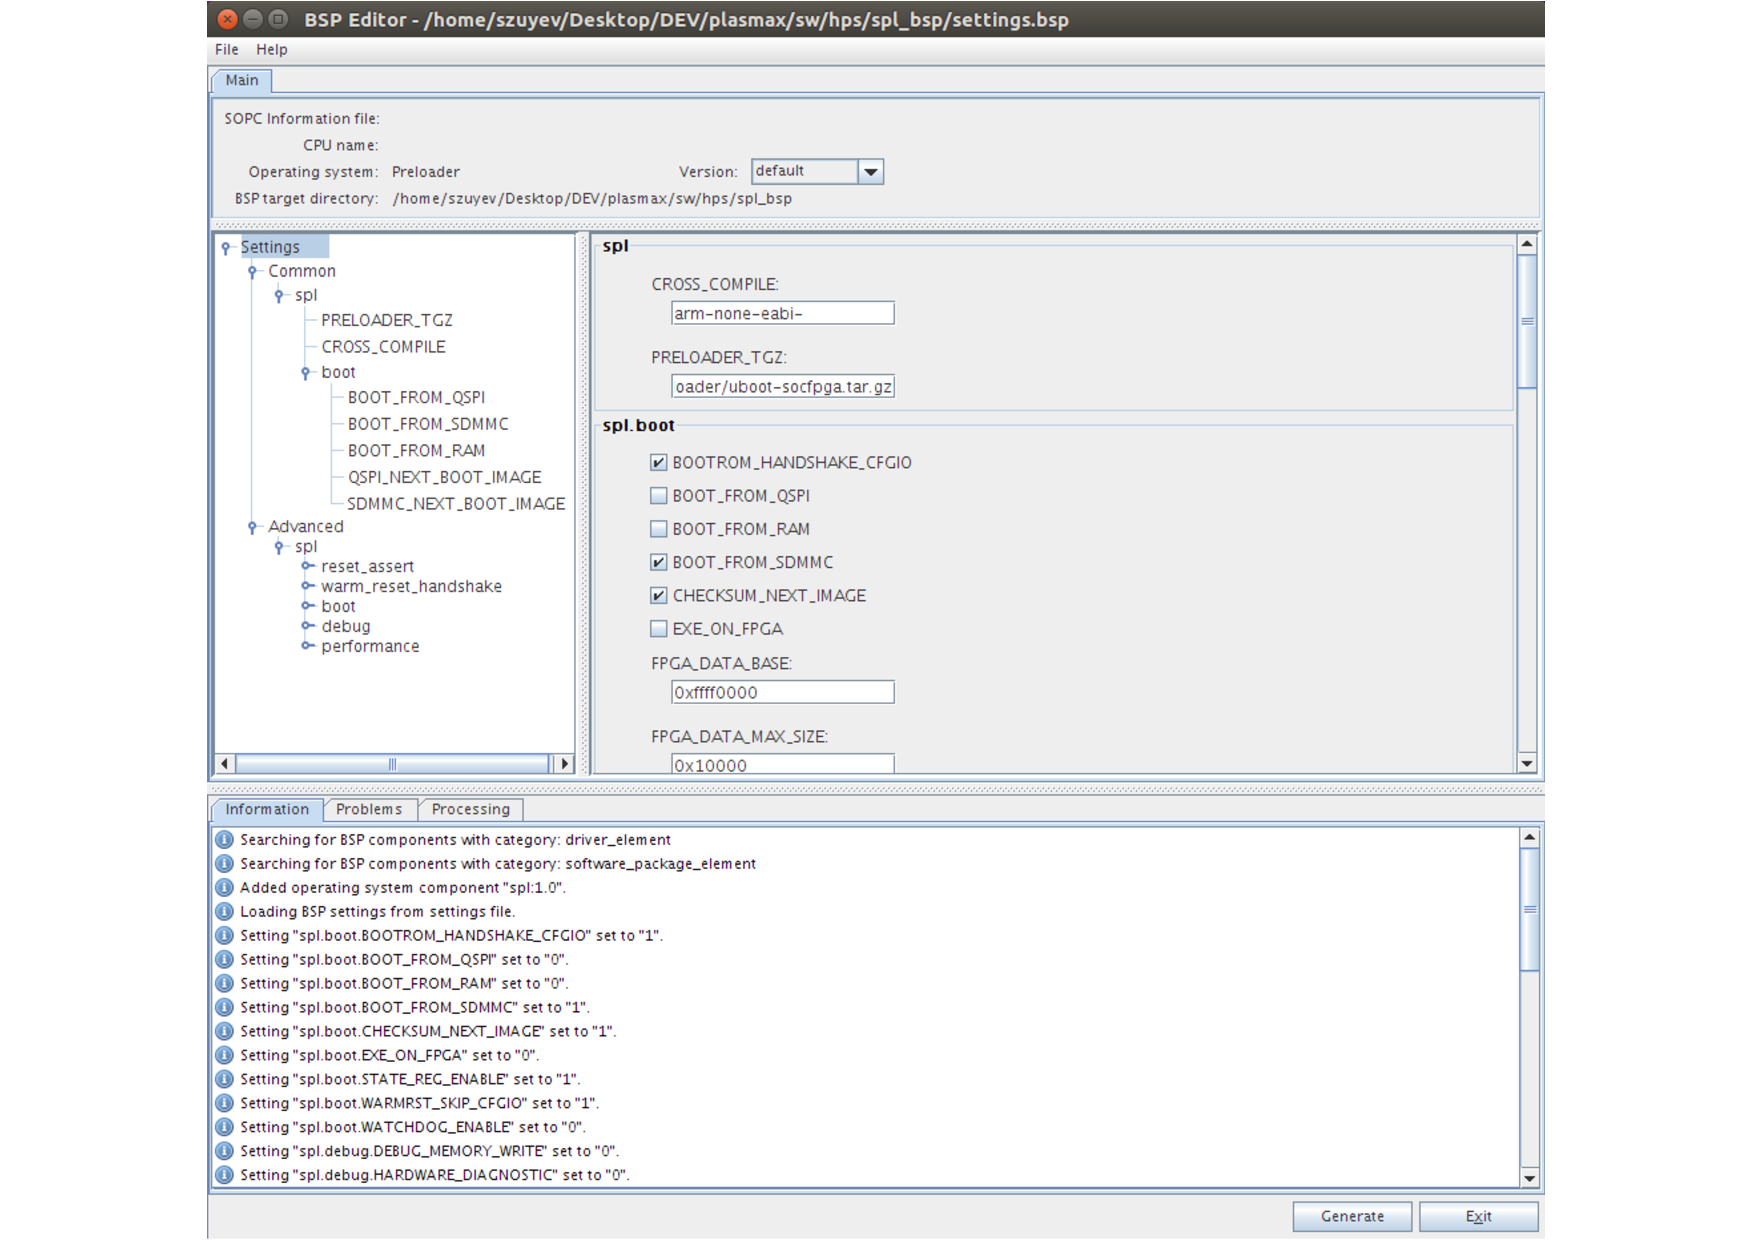
\includegraphics[width=0.9\linewidth]{images/bsp_editor}
		\caption{Parametrisierung}
		\label{fig:bsp_editor_params}
	\end{subfigure}
	\caption{BSP-Editor}
	\label{fig:bsp_editor}
\end{figure}

%\begin{figure}[!htbp] 
%	\centering
%	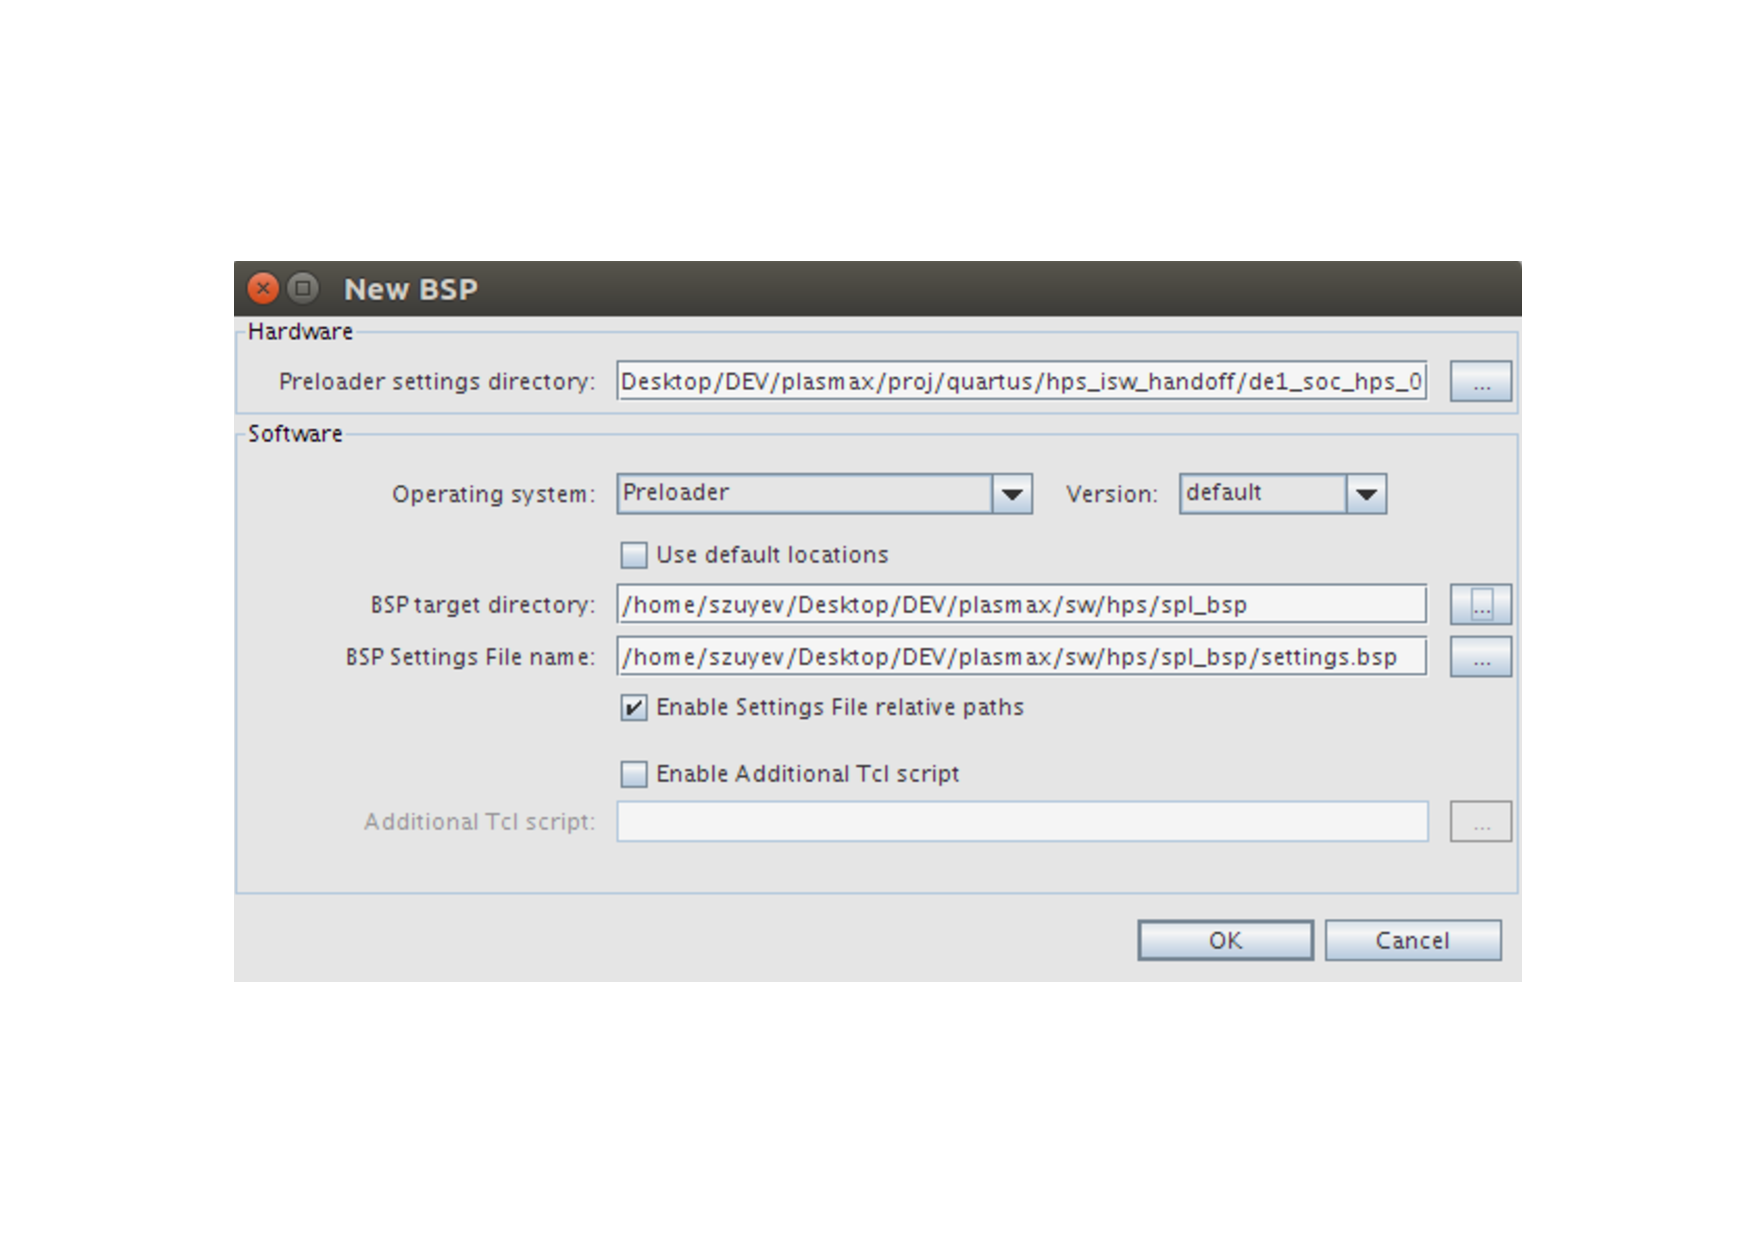
\includegraphics[width=0.8\linewidth]{images/bsp_editor_handoff}
%	\caption{BSP-Editor: Konfiguration eines neuen BSP}
%	\label{fig:bsp_editor_handoff}
%\end{figure}

Im Hauptfenster des \gls{BSP}-Editors (siehe \cref{fig:bsp_editor_params}) werdem die Parameter \texttt{spl\-.performance\-.SERIAL\-\_SUPPORT} und \texttt{spl.reset\-\_assert\-.FPGA\-\_DMA[0-7]} aktiviert, und die Parameter \texttt{spl\-.boot\-.WATCHDOG\-\_ENABLE} und \texttt{spl\-.warm\-\_reset\-\_handshake\-.SDRAM} deaktiviert. 
%\begin{figure}[!htbp] 
%	\centering
%	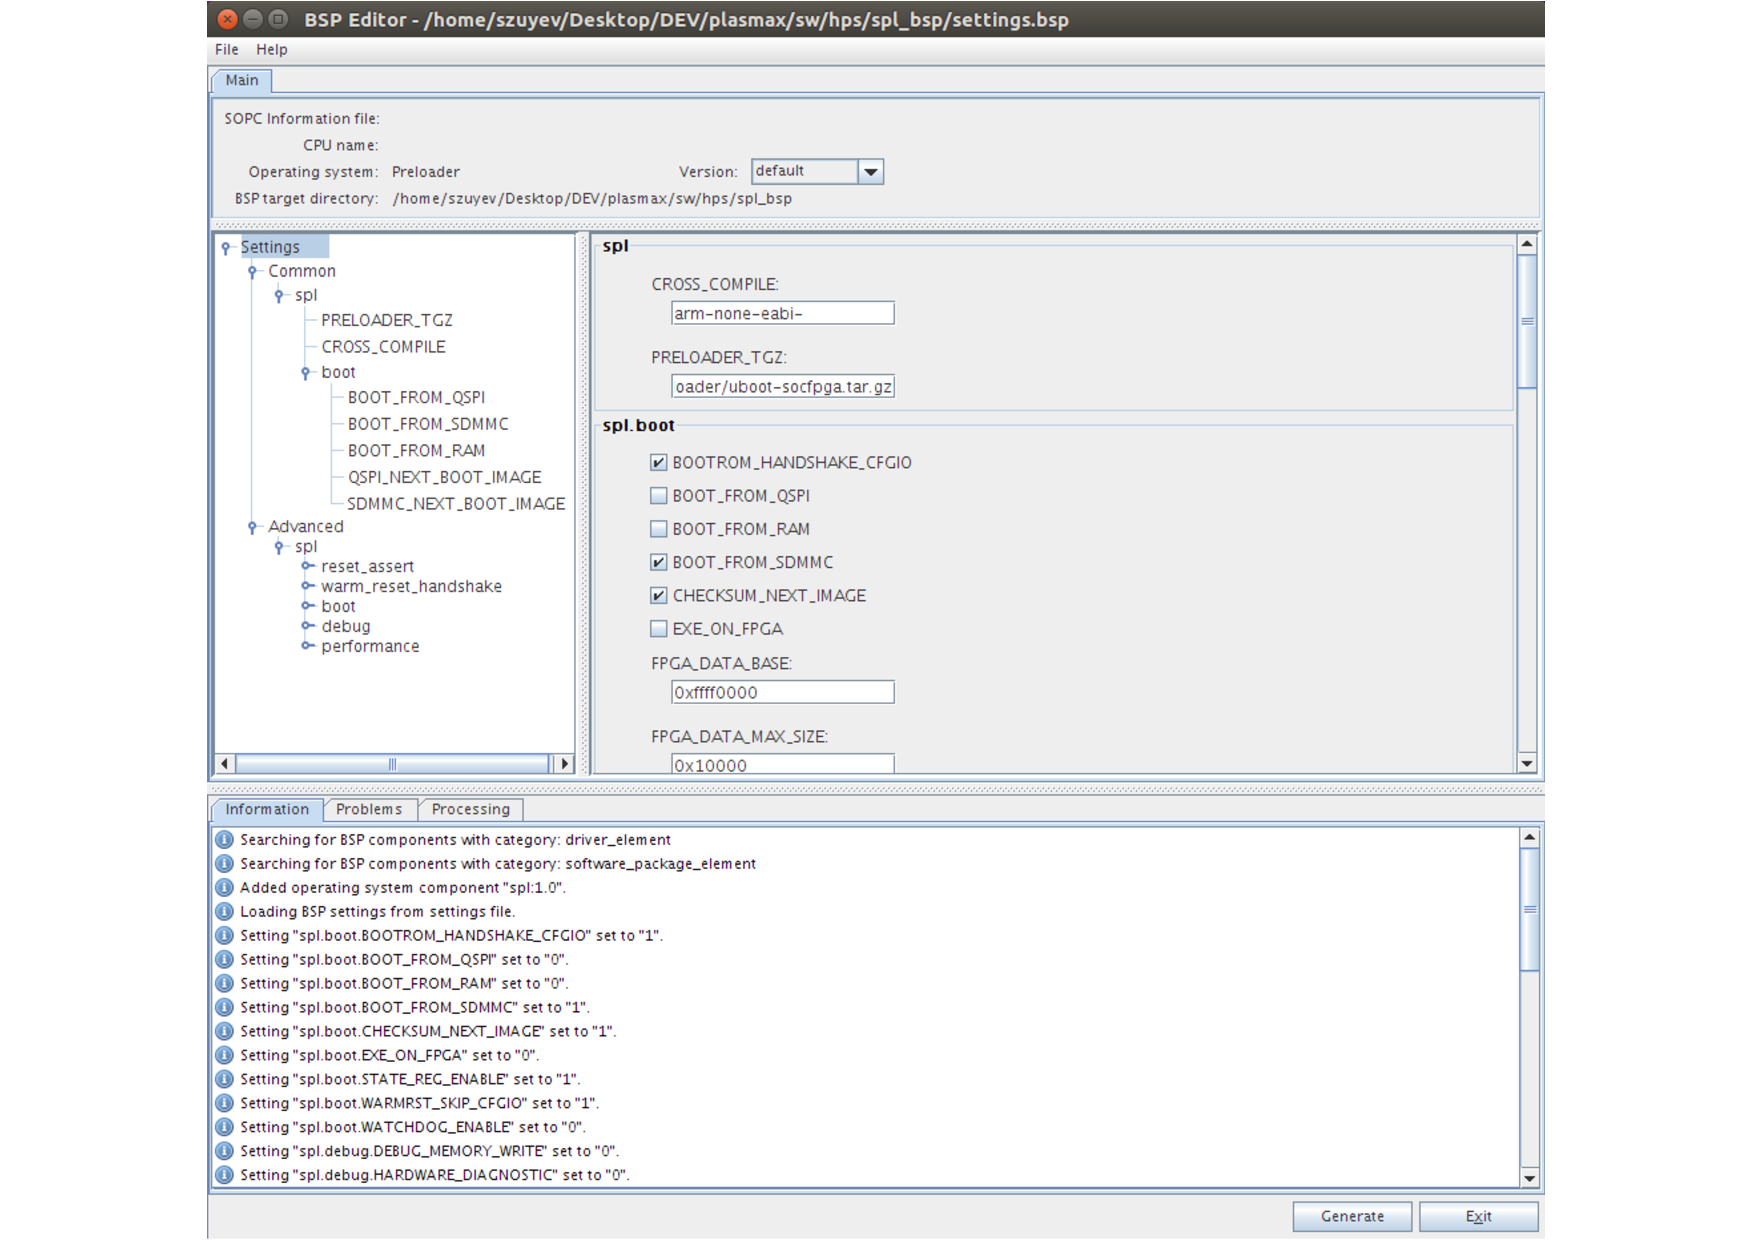
\includegraphics[width=0.8\linewidth]{images/bsp_editor}
%	\caption{BSP-Editor: Parametrisierung}
%	\label{fig:bsp_editor}
%\end{figure}

Im nächsten Schritt wird der Preloader generiert. Im Ausgabeverzeichnis befindet sich der generierte Preloader und nach Ausführung des Befehls \texttt{make uboot} auch der \enquote{U-Boot}-Bootloader. In der Datei \texttt{uboot-socfpga/include/configs/socfpga\_common.h} werden die Konfigurationsvariablen \texttt{mmcloadpart} mit \enquote{2textbackslash{}0} und \texttt{callscript} mit \enquote{if fatload mmc 0:\$mmcloadpart \$fpgadata \$scriptfile} parametrisiert. 

%Zusätzlich wird ein Boot-Skript entworfen:
%\begin{code}	
%	\begin{minted}[breaklines, autogobble]{text}
%	fatload mmc 0:${mmcloadpart} $fpgadata plasma_soc.rbf;
%	fpga load 0 $fpgadata $filesize;
%	run bridge_enable_handoff;
%	
%	echo -- Setting Env Variables --
%	setenv fdtimage socfpga_cyclone5_de1_soc.dtb;
%	setenv mmcroot /dev/mmcblk0p2;
%	setenv mmcload 'mmc rescan;${mmcloadcmd} mmc 0:${mmcloadpart} ${loadaddr} ${bootimage};${mmcloadcmd} mmc 0:${mmcloadpart} ${fdtaddr} ${fdtimage};';
%	setenv mmcboot 'setenv bootargs earlyprintk debug console=ttyS0,115200 root=${mmcroot} rootfstype=ext4 rw rootwait mem=768M; bootz ${loadaddr} - ${fdtaddr}';
%	
%	run mmcload;
%	run mmcboot;
%	\end{minted}
%	
%	\caption{Boot-Skript}
%	\label{lst:boot_script}
%\end{code}
%
%Nach diesen Anpassungen werden der Preloader, der \enquote{U-Boot}-Bootloader und das Boot-Skript kompiliert.

\subsection{Kernel}
\label{sec:impl_kernel}

Für das DE1-SoC wird ein moderner Linux-Kernel konfiguriert und kompiliert, da die vorgefertigten Systemabbilder von Terasic und Altera alte Kernel mit Devicetree-Kompatibilitätsproblemen einsetzen.

Das \enquote{linux-socfpga}-Repository \cite{website:linux_socfpga_repository} wird geklont und das Release 4.9.78-ltsi ausgecheckt.
Mit der Altera Embedded Command Shell \cite[14]{manual:using_linux_on_de1_soc} wird eine Cross-Compiler Umgebung vorbereitet und der Kernel mit dem menugeführtem Konfigurationswerkzeug \texttt{nconfig} konfiguriert. 

Im Konfigurator werden  Parameter wie z.B der Hostname gesetzt, Gerätetreiber und Debug-Möglichkeiten ausgewählt und  Altera-spezifische Einstellungen vorgenommen. Aus der Kernel-Konfiguration wird eine \texttt{defconfig}-Datei generiert, die wie eine Patch-Datei jederzeit auf einer Kernel-Konfiguration angewandt werden kann. 

Kompiliert werden ein zImage und alle ausgewählten Kernel-Module.
%Die \texttt{defconfig}-Datei kann im \cref{lst:kernel_config_defconfig} eingesehen werden.

%Das \enquote{linux-socfpga}-Repository \cite{website:linux_socfpga_repository} wird geklont und das Release 4.9.78-ltsi ausgecheckt.
%\begin{minted}[breaklines, autogobble]{text}
%git clone https://github.com/altera-opensource/linux-socfpga.git
%git checkout rel_socfpga-4.9.78-ltsi_18.08.01_pr -b 4.9.78-ltsi
%\end{minted}
%
%Die Altera Embedded Command Shell \cite[14]{manual:using_linux_on_de1_soc}  wird gestartet und Umgebungsvariablen für den Cross-Compiler gesetzt:
%\begin{minted}[breaklines, autogobble]{text}
%export ARCH=arm 
%export CROSS_COMPILE=arm-linux-gnueabihf-
%\end{minted}
%
%Die Kernel-Standardkonfiguration für Cyclone V \gls{SoC}-\glspl{FPGA} wird geladen:
%\begin{minted}[breaklines, autogobble]{text}
%make socfpga_defconfig
%\end{minted}
%
%Weitere Konfiguration erfolgt mit \texttt{nconfig}:
%\begin{minted}[breaklines, autogobble]{text}
%make nconfig
%\end{minted}
%
%Die menugeführte Konfigurationsoberfläche kann wie in \cref{fig:linux_kernel_config_fpga_bridge} aussehen. 
%\begin{figure}[!htbp]
%	\centering
%	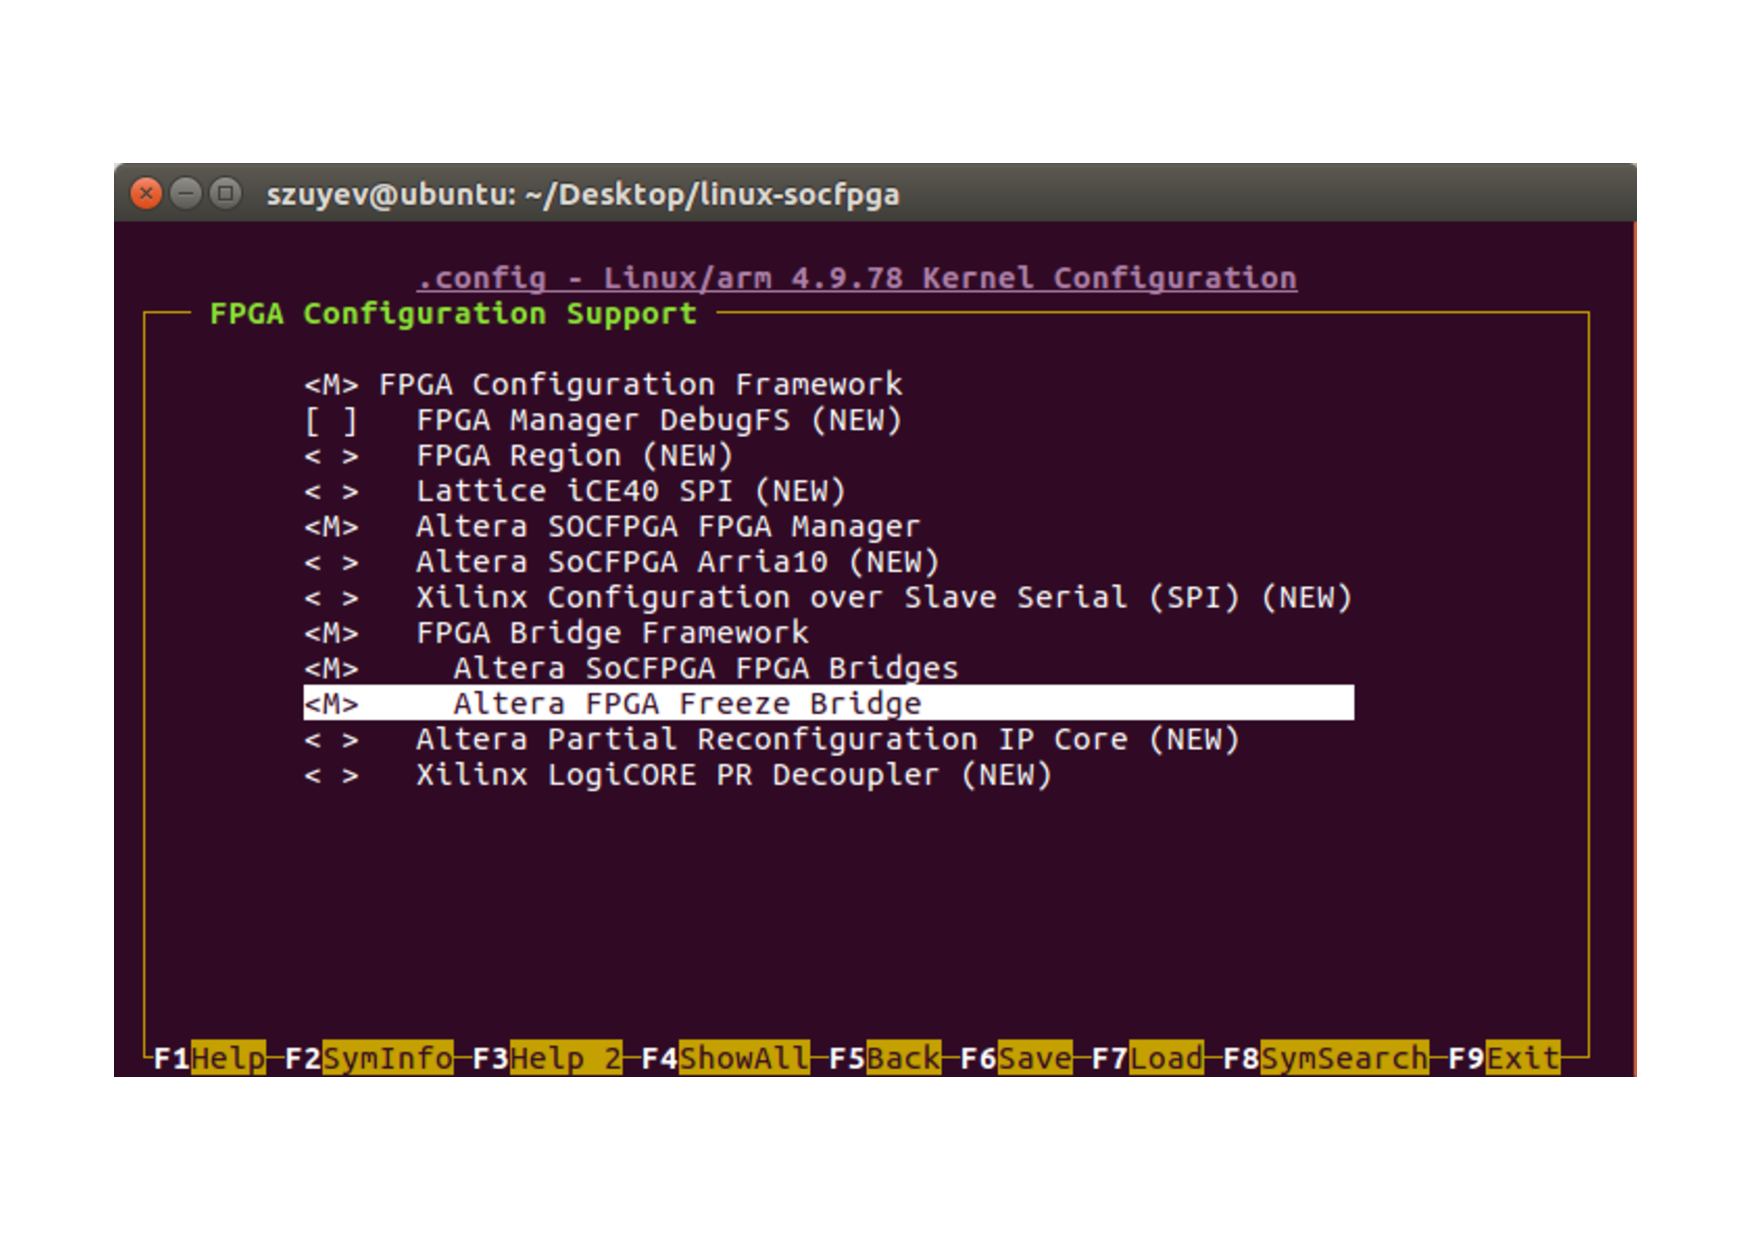
\includegraphics[width=0.6\linewidth]{images/linux_kernel_config_fpga_bridge}
%	\caption{Ausschnitt aus der Kernel-Konfiguration}
%	\label{fig:linux_kernel_config_fpga_bridge}
%\end{figure}

%Im Konfigurator werden  Parameter wie z.B der Hostname gesetzt, Gerätetreiber und Debug-Möglichkeiten ausgewählt und insbesondere Altera-spezifische Einstellungen vorgenommen. Aus der Kernel-Konfiguration wird eine \texttt{defconfig}-Datei generiert, welche die nur vorgenommenen Änderungen beinhaltet und jederzeit an einem anderen Kernel-Quelltext angewandt werden kann. Die \texttt{defconfig}-Datei kann im \cref{lst:kernel_config_defconfig} eingesehen werden.

\subsection{Systemabbild}

Ein im Altera University Program verfügbares Systemabbild\footnote{\url{ftp://ftp.altera.com/up/pub/Altera_Material/16.0/Linux_Images/}} für das DE1-SoC-Board wird als Basis für eigene Anpassungen verwendet. In diesem Abbild ist ein Ubuntu 12.04 Betriebssystem vorkonfiguriert. Um eine auf das DE1-SoC-Board mit einem Plasma-\gls{SoC} zugeschnittene Betriebssystem-Distribution mit graphischer Oberfläche zu erstellen, muss nur wenig Aufwand betrieben werden.

Es werden der Preloader, der \enquote{U-Boot}-Bootloader, das Boot-Skript, der kompilierte Devicetree sowie der Kernel mit den Kernel-Modulen durch neue Komponenten aus \cref{sec:impl_bootloader}, \cref{sec:impl_kernel} und \cref{sec:impl_devicetree} ersetzt.
%
%\begin{figure}[!htbp] 
%	\centering
%	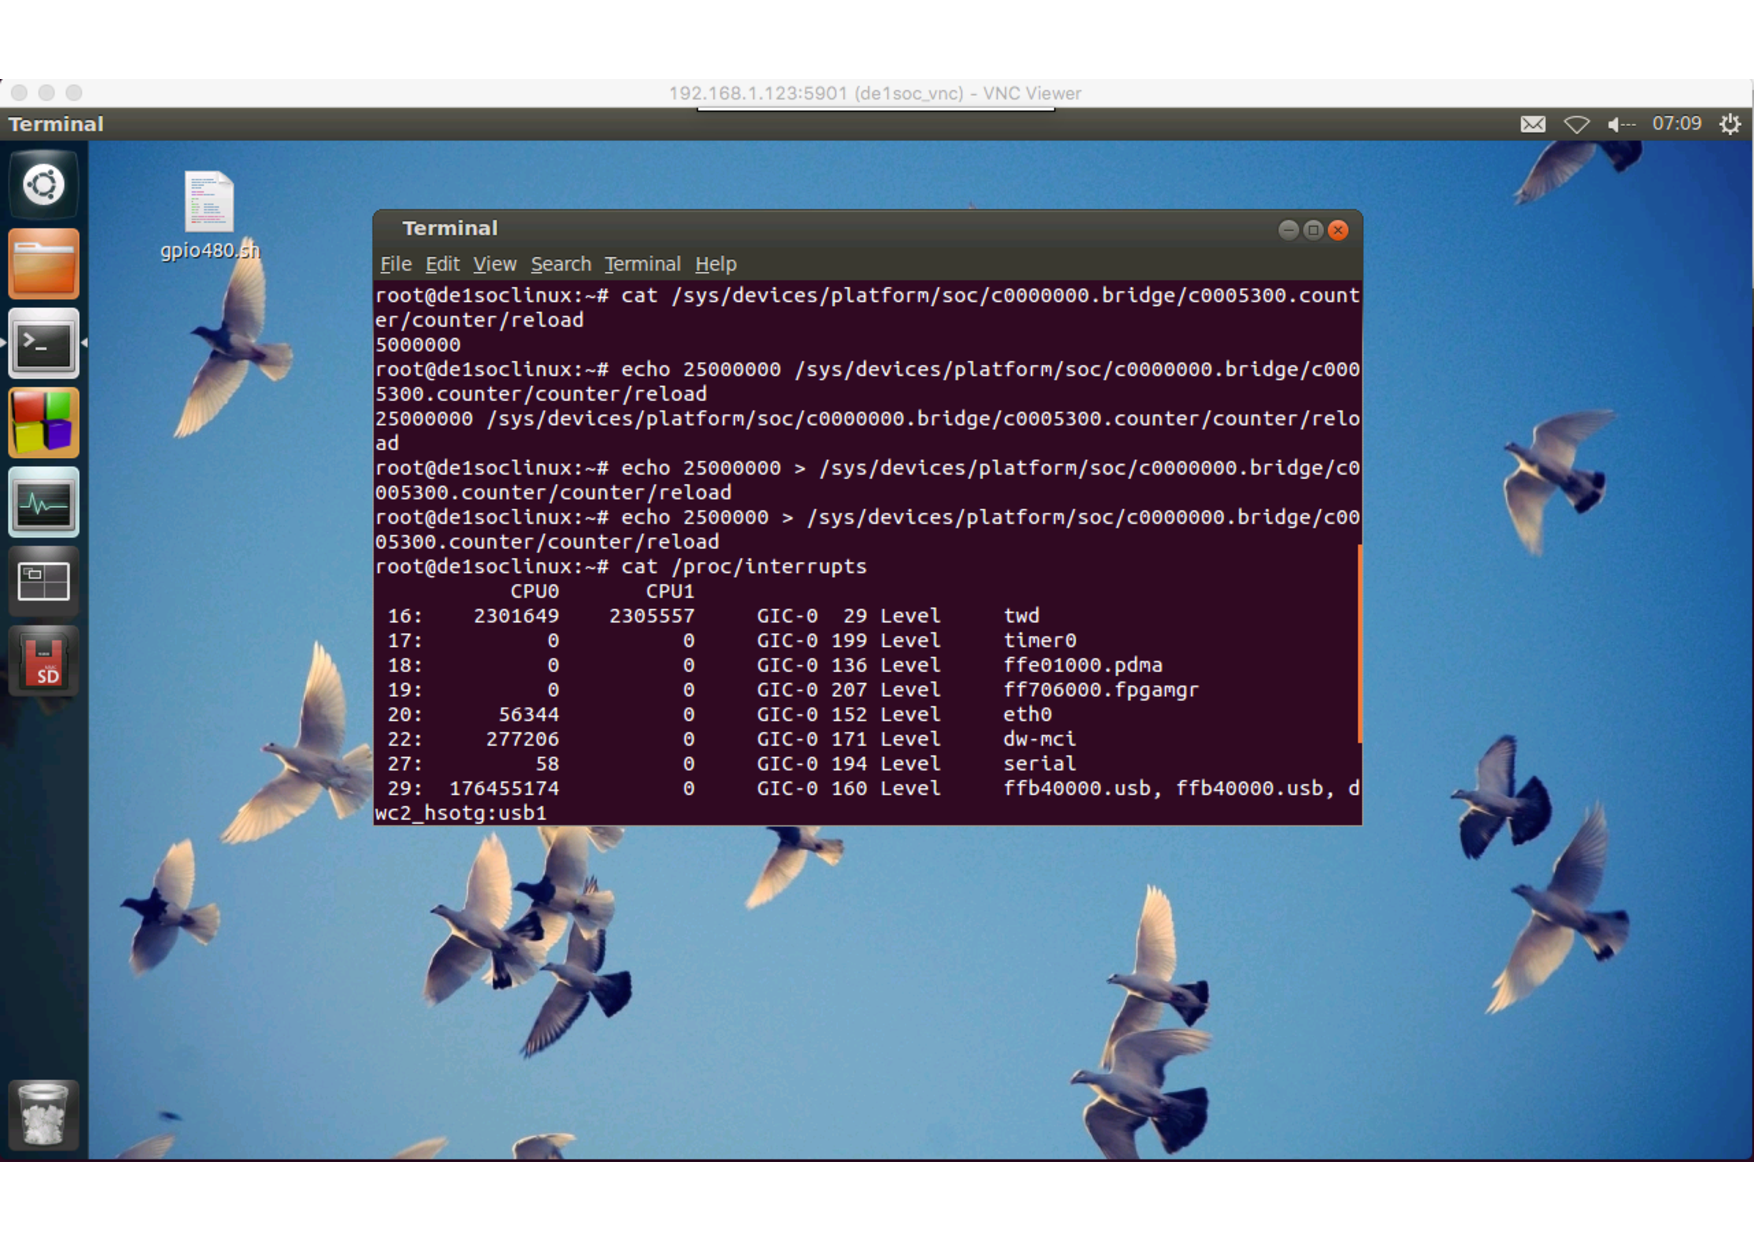
\includegraphics[width=0.8\linewidth]{images/ubuntu_with_custom_kernel}
%	\caption{Ubuntu 12.04-Distribution mit angepasstem Linux 4.9.78 Kernel}
%	\label{fig:ubuntu_with_custom_kernel}
%\end{figure}

\section{Entwicklung von Linux-Anwendungen für das HPS}
\label{sec:impl_develop_linux_sw_for_de1_soc}

Aufbauend auf einem Beispielprogramm zur Kommunikation mit dem \gls{FPGA} \cite[16ff]{manual:using_linux_on_de1_soc} werden zwei mit dem Plasma-\gls{SoC} kommunizierende Linux-Anwendungen entwickelt: \enquote{SysID} und \enquote{LED Pattern Manager}.

Für einen Zugriff auf Hardware-Ressourcen müssen unter einem Betriebssystem mit virtuellem Speichermanagement physische Adressen in virtuelle abgebildet werden. Das Linux-Betriebssystem ist ein System mit virtuellem Speichermanagement und bietet die zur Adressabbildung notwendige Funktionalität an. 

Mit einem Aufruf von \texttt{open("/dev/mem", (O\_RDWR | O\_SYNC))} wird zunächst das Memory-Device zum Lesen und Schreiben geöffnet, und mit einem Aufruf von \texttt{mmap} werden die physischen Adressräume der übergebenen \gls{Bridge}-Adressen in den virtuellen Adressraum abgebildet. 

In beiden Anwendungen wird eine \texttt{goto}-basierte Fehlerbehandlung umgesetzt. Dadurch werden sowohl im Fehlerfall als auch im normalen Betrieb die Ressourcen in der korrekten Reihenfolge wieder freigegeben. Außerdem wird zur Ausgabe von Fehlermeldungen die Funktion \texttt{void perror(const char *s)} verwendet. Diese Funktion gibt nicht nur die benutzerdefinierte Fehlermeldung aus, sondern  auch die Beschreibung der Fehlerursache \cite[50f]{book:c_and_linux}.

Die Anwendung \enquote{SysID} wird zum Testen der Lightweight HPS2FPGA- und der Wishbone{$\leftrightarrow$}Avalon-\glspl{Bridge} entwickelt. Es findet ausschließlich ein Lesezugriff auf die im SysID-IP-Core fest hinterlegten System-ID und Zeitstempel. Diese werden ausgelesen und im Standard-Ausgabestream ausgegeben. 

Die Anwendung \enquote{LED Pattern Manager} wird zum Testen der Lightweight HPS2FPGA, HPS2FPGA- und der Wishbone{$\leftrightarrow$}Avalon-\glspl{Bridge} entwickelt. Es finden sowohl Lese- als auch Schreibzugriffe statt. 

Analog zur \enquote{SysID}-Anwendung werden die System-ID und der Zeitstempel aus dem SysID-IP-Core ausgelesen und im Standard-Ausgabestream ausgegeben. 

Zusätzlich werden jede \SI{500}{\milli\second} die Werte des Schalter- und Tasterblocks über die HPS2FPGA-\gls{Bridge} ausgelesen und ausgewertet. Der Wert des Schalterblocks wird in den externen \gls{RAM} des Plasma-\gls{SoC} geschrieben, und vom dort ausgeführtem Programm als LED-Muster angezeigt. Der Tasterblock ist active-low: im Normalzustand liegt eine logische \enquote{1} an, und bei Aktivierung liegt eine logische \enquote{0} an. Durch bitweise Negation und Maskierung der unteren 4 Bit wird ein active-high Wert ermittelt.

Wird \textit{KEY3} betätigt, so ändert sich die Bewegungsrichtung des LED-Musters zur Linksbewegung, \textit{KEY2} hingegen bewirkt eine Rechtsbewegung.  
 Das Drücken des \textit{KEY1}-Tasters halbiert das Timer-Intervall, sodass die Bewegungsgeschwindigkeit verdoppelt wird. Das Betätigen des \textit{KEY0} verlangsamt die Bewegung durch Verdoppelung des Timer-Intervalls.  
  
 Da die Schalter und Taster in einer Endlosschleife abgefragt werden und keine Konsoleninteraktion genutzt wird, kann die Anwendung nicht ordentlich beendet werden. Damit die Ressourcen trotzdem freigegeben werden, wird ein benutzerdefinierter Signal-Handler für das Interrupt-Signal (\texttt{SIGINT}) eingeführt. Dafür wird die Funktion \texttt{signal(int signum, void *handler())} verwendet \cite[88f]{book:c_and_linux}. 


\section{Entwicklung eines Linux-Treibers für das HPS}
\label{sec:impl_develop_linux_drivers_for_de1_soc}

Um eine gute Integration des Plasma-\gls{SoC} und dem Linux-Betriebssystem auf dem \gls{HPS} zu demonstrieren, wird ein einfacher Treiber für über Wishbone angebundene Zähler im Plasma-\gls{SoC} entwickelt. Mit diesem Treiber wird der Zugriff auf das Reload-Register des Zählers über sysfs ermöglicht. Als Vorlage dient der Altera SysID-Treiber \cite[Version~4.9.78-ltsi, \texttt{drivers/misc/altera\_sysid.c}]{website:linux_socfpga_repository}.

Im \cref{sec:impl_devicetree} wurde bereits eine Devicetree-Datei für den Plasma-\gls{SoC} auf dem DE1-SoC-Board entworfen. Für diesen Abschnitt sind die im \cref{lst:custom_dts_plsoc_devices} dargestellten Definitionen sämtlicher am Wishbone-Bus angebundener Komponenten des Plasma-\gls{SoC} von hoher Bedeutung. Über den \texttt{compatible}-Eintrag wird der Treiber an alle im Devicetree definierten Geräte mit übereinstimmenden \texttt{compatible}-Schlüsselwert gebunden, in diesem Fall an die Zähler.

Bei der Registrierung des Treibers wird ein sysfs-Verzeichnis im übergeordneten Bus-Verzeichnisses erstellt. In diesem Verzeichnis kann der Treiber eine Schnittstelle exportieren, sodass eine Ansteuerung aus dem Userspace möglich wird \cite[Version~4.9.78-ltsi, \texttt{Documentation/driver-model/driver.txt, Zeile~131}]{website:linux_socfpga_repository}.

Um eine Schnittstelle im sysfs zu exportieren, müssen Attribute und dazugehörige Getter- und Settter (in der Kernel-Terminologie: \texttt{show} und \texttt{store}) implementiert werden \cite[Version~4.9.78-ltsi, \texttt{Documentation/filesystems/sysfs.txt}, Zeile~233]{website:linux_socfpga_repository}. 

Sobald eine Bindung zu einem Zähler im Plasma-\gls{SoC} möglich wird, findet automatisch ein Aufruf der \enquote{plsoc\_counter\_probe}-Methode statt. Der Adressraum des Zählers wird mit \texttt{platform\_get\_resource} abgerufen und mit \texttt{devm\_ioremap\_resource} auf den mit \texttt{devm\_kzalloc} allozierten und initialisierten Speicher abgebildet. Abschließend werden die Attribute mit \texttt{sysfs\_create\_group} zum sysfs hinzugefügt, sodass ein Zugriff auf den Zähler über \texttt{/sys/devices/platform/...} möglich wird. 

Die \enquote{plsoc\_counter\_remove}-Methode wird beim Entladen des Treibers bzw. Deaktivierung des Zählers aufgerufen. Es werden die sysfs-Einträge entfernt und der Adressraum des Zählers vom Treiber entbunden.

%\todo{Compilation}
\begin{figure}[!htbp] 
	\centering
	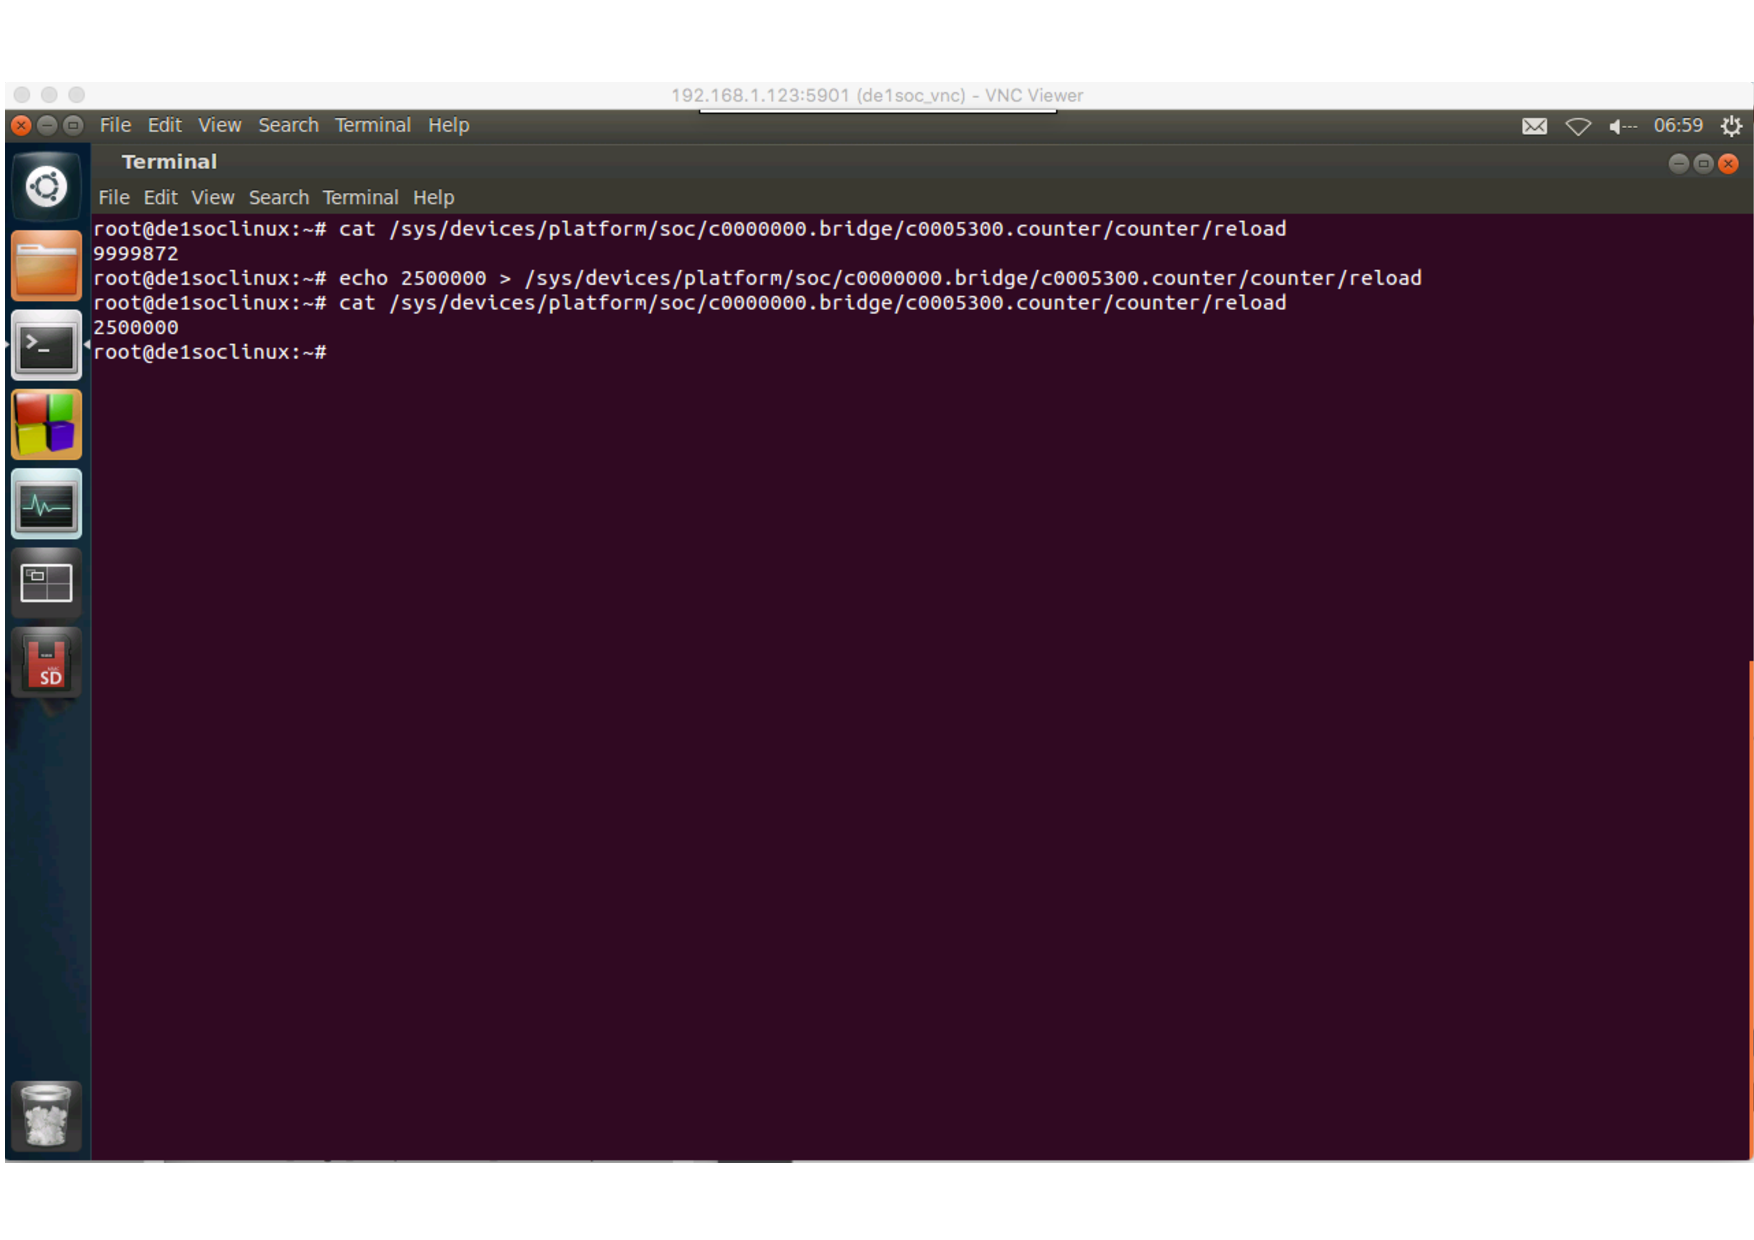
\includegraphics[width=0.9\linewidth]{images/driver_sysfs}
	\caption[Zugriff auf das Reload-Register aus dem Terminal]{Zugriff auf das Reload-Register aus dem Terminal. Es wird der erste Zähler mit der Wishbone-Adresse \texttt{0x5300} angesteuert.}
	\label{fig:driver_sysfs}
\end{figure}
	\chapter{Ergebnisse und Ausblick}
\label{cha:synopsis}

In diesem Kapitel werden die Ergebnisse dieser Bachelorarbeit zusammengefasst und künftige Entwicklungsmöglichkeiten erörtert. Es werden sowohl neue Möglichkeiten, als auch Einschränkungen des entstandenen Systems besprochen. 

\section{Zusammenfassung}

Mit der Einführung des Wishbone-Bus wird ein Ausbau des Plasma-Systems mit eigens entwickelten Komponenten und frei verfügbaren IP-Cores von OpenCores deutlich vereinfacht, da vorher keine standardisierte Schnittstelle zur Plasma-\gls{CPU} gegeben war. 

Die Erweiterung des Plasma-Systems um eine Wishbone{$\leftrightarrow$}Avalon-\gls{Bridge} ermöglicht die Integration als IP-Core in Altera/Intel-\gls{FPGA}-basierte Projekte. Erst mit Einführung dieser Bridge wird eine einfache Anbindung der DE1-SoC-spezifischen Komponenten, wie dem verlötetem SDRAM-Chip, der \gls{ARM}-\gls{CPU}, Schalter, Taster, LEDs und 7-Segmentanzeigen, an das Plasma-\gls{SoC} möglich. 

Durch die Anbindung des externen SDRAM-Chips erhöht sich der im Plasma-System verfügbare Arbeitsspeicher von \SI{8}{\kilo\byte} 
auf über \SI{64}{\mega\byte}, was die Verarbeitung größerer Datenmengen und komplexere Anwendungen ermöglicht. 

Korrekturen des Wishbone-Busses und die Einführung eines neuen Bus-Arbiters legen den Grundstein für einen ordnungsgemäßen Multi-Master-Betrieb. Das System arbeitet in diesem Modus sobald ein Zugriff auf das Plasma-\gls{SoC} über die Wishbone{$\leftrightarrow$}Avalon-\gls{Bridge} erfolgt. 

Die Erstellung eines Linux-Betriebssystems auf Basis eines vorgefertigten Systemabbilds ist ein wichtiger Schritt zur vollen Nutzung der Möglichkeiten, die ein \gls{SoC}-\gls{FPGA} bietet. Das Betriebssystem wird auf dem \gls{ARM}-Prozessor ausgeführt, und greift über einen Treiber und mehrere Benutzeranwendungen auf das Plasma-\gls{SoC} zu. Um den Zugriff auf das Plasma-\gls{SoC} zu ermöglichen, wurde ein aktueller Linux-Kernel konfiguriert und kompiliert, die Linux-Treiber aktualisiert und eine eigene, auf das DE1-SoC-Board und Plasma-\gls{SoC} zugeschnittene Devicetree-Beschreibung entwickelt. 

Der entwickelte Treiber steuert die Reload-Register der Zähler im Plasma-\gls{SoC} an. 

Leider hat die Bearbeitungszeit nicht mehr ausgereicht, um das Plasma-\gls{SoC} mit einer ausführbaren Datei aus dem Linux-Betriebssystem heraus zu programmieren. Aus dem selben Grund konnten für das Plasma-\gls{SoC} keine Regressionstests auf dem Digilent Zedboard durchgeführt werden. 
  
\section{Ausblick}

Der Wishbone-Bus ist in der einfachsten Variante umgesetzt und unterstützt keine Bursttransfers, atomare \Gls{RMW}-Zyklen und split transactions. Pipelining wurde ebenfalls nicht erprobt, da dafür eine Erweiterung der Wishbone-Slaves notwendig wäre. Für einen performanteren Betriebsablauf könnten diese Features implementiert werden. 

Gegebenenfalls könnte eine Plasma-\gls{SoC} \gls{CSR}-Komponente entwickelt werden, die das Auslesen von Statusflags und Anhalten des Plasma-Prozessors von außen ermöglicht. Ein denkbarer Anwendungsfall wäre die Umprogrammierung, da das Verhalten der Plasma-\gls{CPU} beim Überschreiben des Programmspeichers im laufenden Betrieb derzeit nicht absehbar ist. 

Zudem könnten Linux-Treiber für weitere Komponenten des Plasma-\gls{SoC}, wie z.B. Timer und \glspl{GPIO}, sowie ein Treiber, welcher die Speicher des Plasma-\gls{SoC} als eine konsekutive Datei abbildet, entwickelt werden. 

Basierend auf dem \gls{ELF}-Converter-Skript könnte für den Plasma-Prozessor ein \gls{ELF}-Loader entwickelt werden, sodass eine Programmierung aus dem Linux-Betriebssystem heraus möglich wird. 

Da dem Plasma-\gls{SoC} nun deutlich mehr Arbeitsspeicher zur Verfügung steht, wäre die Portierung eines Embedded-Betriebssystems wie z.B FreeRTOS\footnote{\url{https://www.freertos.org/}} oder Zephyr\footnote{\url{https://www.zephyrproject.org/}} eine erwägenswerte Verbesserungsmöglichkeit. 

	
	
	\printbibliography[title={Literaturverzeichnis}]	
	\appendix
	\chapter{Übersicht über elektronische Anhänge}

\begin{easylist}[itemize]
	& Bachelorarbeit in elektronischer Form
	& Bitstreams
	&& plasma\_soc.rbf
	& dts
	&& socfpga\_cyclone5\_de1\_soc.dtb
	&& socfpga\_cyclone5\_de1\_soc.dts
	&& socfpga\_cyclone5.dtsi
	&& socfpga.dtsi
	&& skeleton.dtsi
	& Plasma-SoC - Quelltexte
	&& proj - Vivado und Quartus Projektdateien
	&& rtl - Hardwarebeschreibung
	&& sw - Software
	&& tb - Testbenches
	&& dependencies 
	&&& KebabOS - Firmware-Quellcode
	&&& PlasmaConvert - ELF-Converter
	& Referenzen
	& Webquellen
	& README.md
	& linux-socfpga-socfpga-4.9.78-ltsi.zip
	&& Linux-Kernel-Quelltexte 4.9.78-ltsi
	&&& Als ZIP mitgeliefert, da auf dem MacOS das Dateisystem nicht Case-Sensitiv ist. 
	&& ubuntu-4.9.78.img.gz - modifiziertes Linux-Systemabbild
	&&&  Komprimiertes Image, zum direkten Beschreiben eines Gerätes bitte \texttt{gunzip -c ubuntu-4.9.78.img.gz | pv | sudo dd of=/dev/sdf bs=1M} ausführen
\end{easylist}
%\textsl{}
%
%\chapter{Serielle Verbindung}
%
%Die serielle Verbindung wird mit folgenden Parametern aufgebaut: 
%\begin{easylist}[itemize]
%	& Übertragungsgeschwindigkeit: 115200 Baud
%	& Datenbits: 8
%	& Stoppbits: 1
%	& Parität: keine
%	& Datenflusssteuerung: keine
%\end{easylist}
%
%Eine mögliche Konfiguration für Putty ist in \cref{fig:putty} dargestellt. Sobald die Verbindung erfolgreich aufgebaut wird, sollte der Terminal wie auf \cref{fig:putty_serial_connected} aussehen. 
%
%\begin{figure}[!htbp]
%	\centering
%	\begin{subfigure}{.5\textwidth}
%		\centering
%		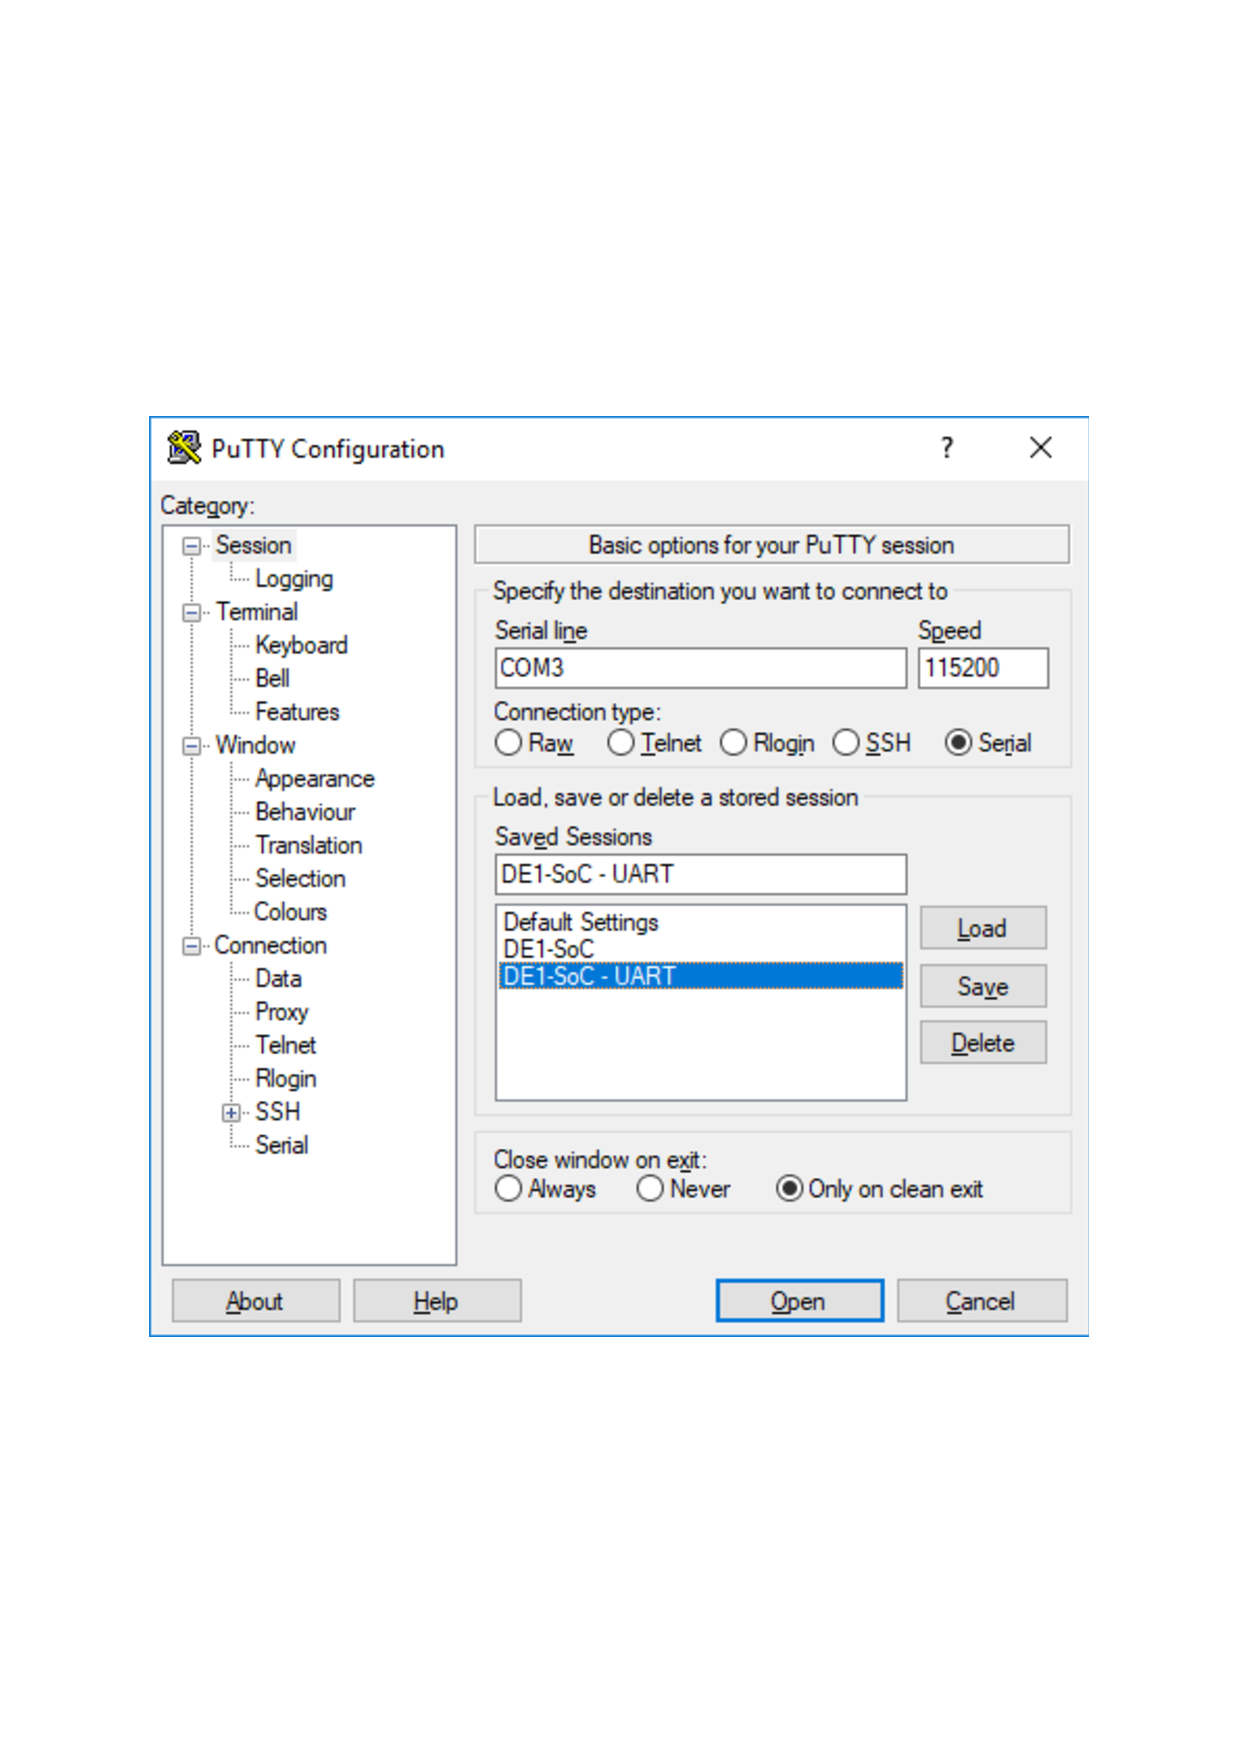
\includegraphics[width=0.9\linewidth]{images/putty_serial}
%		\caption{Grundeinstellungen}
%		\label{fig:putty_serial}
%	\end{subfigure}%
%	\begin{subfigure}{.5\textwidth}
%		\centering
%		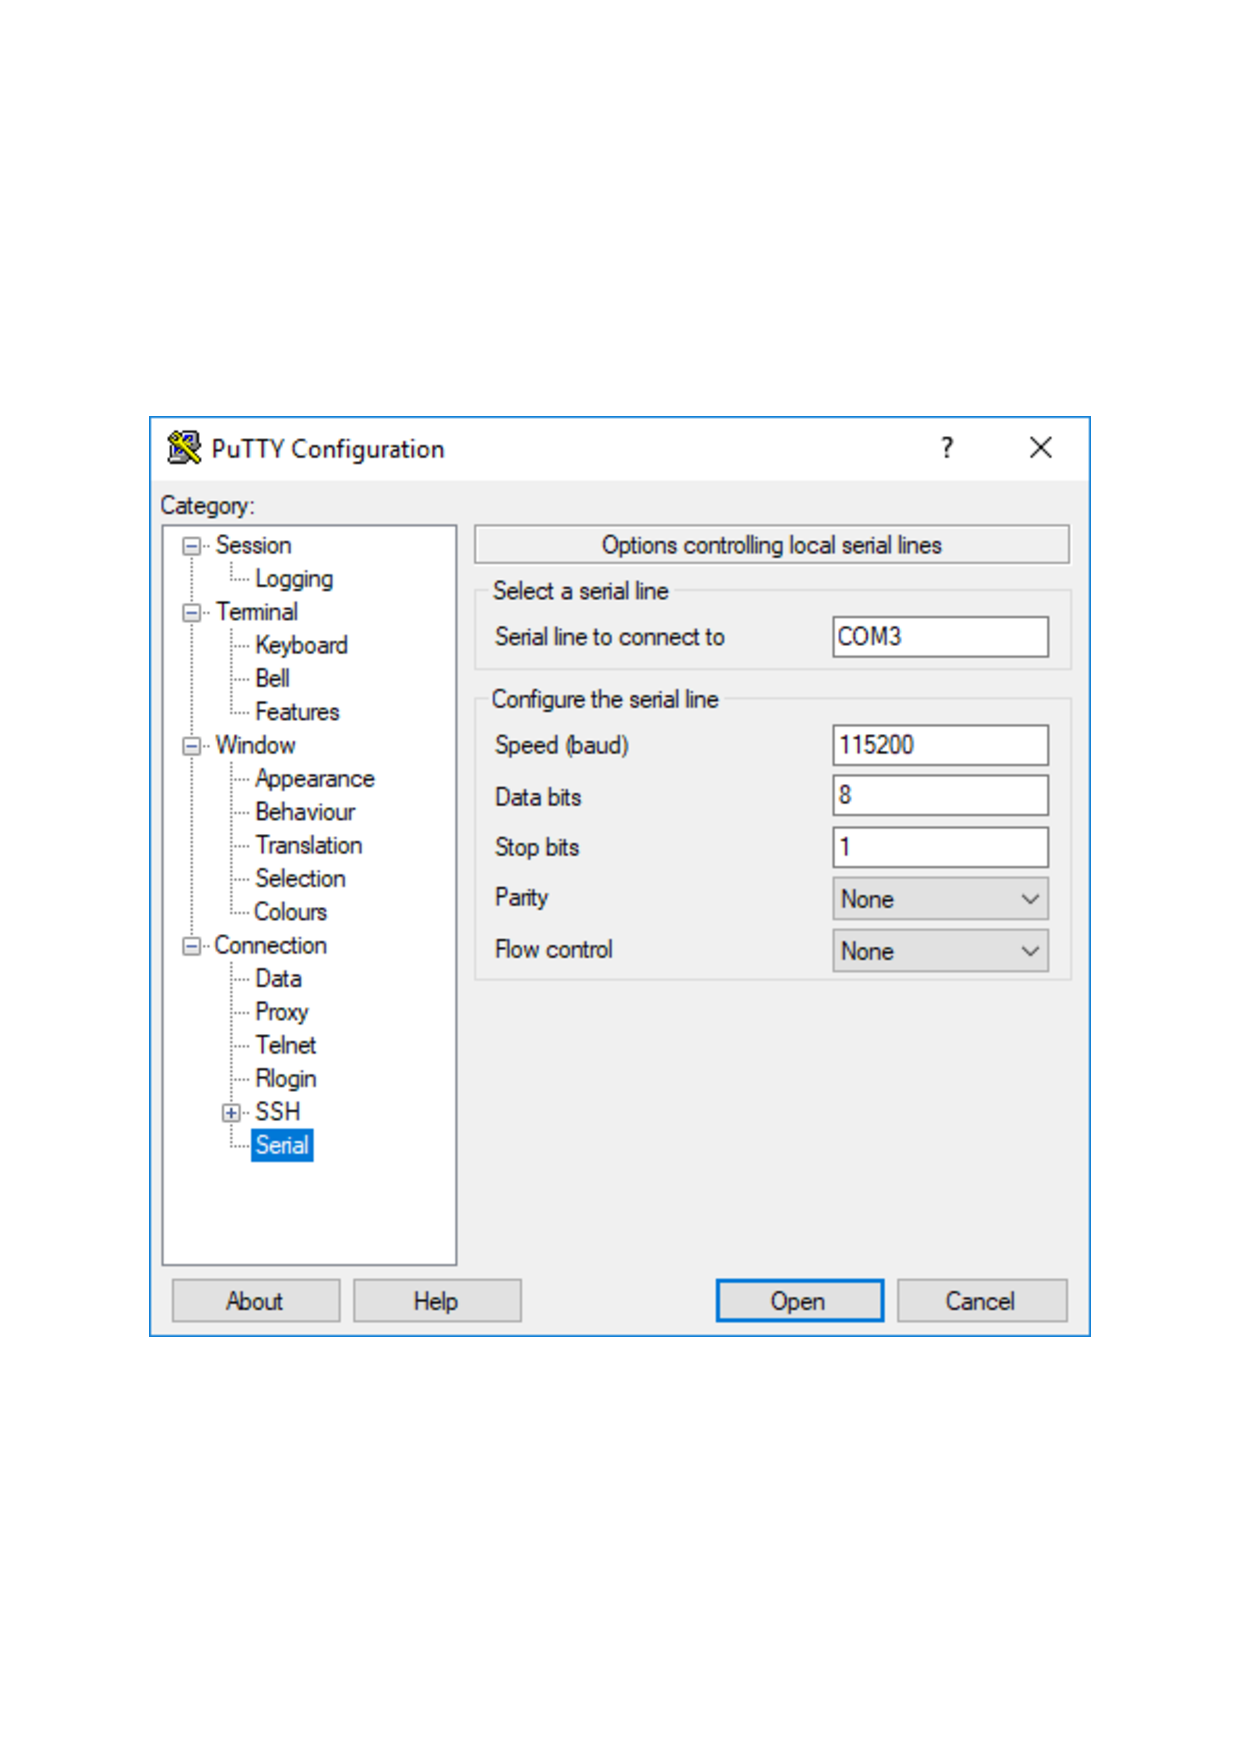
\includegraphics[width=0.9\linewidth]{images/putty_serial_params}
%		\caption{Erweiterte Einstellungen}
%		\label{fig:putty_serial_params}
%	\end{subfigure}
%	\caption{Putty-Konfiguration}
%	\label{fig:putty}
%\end{figure}
%
%\begin{figure}[!htbp]
%	\centering
%	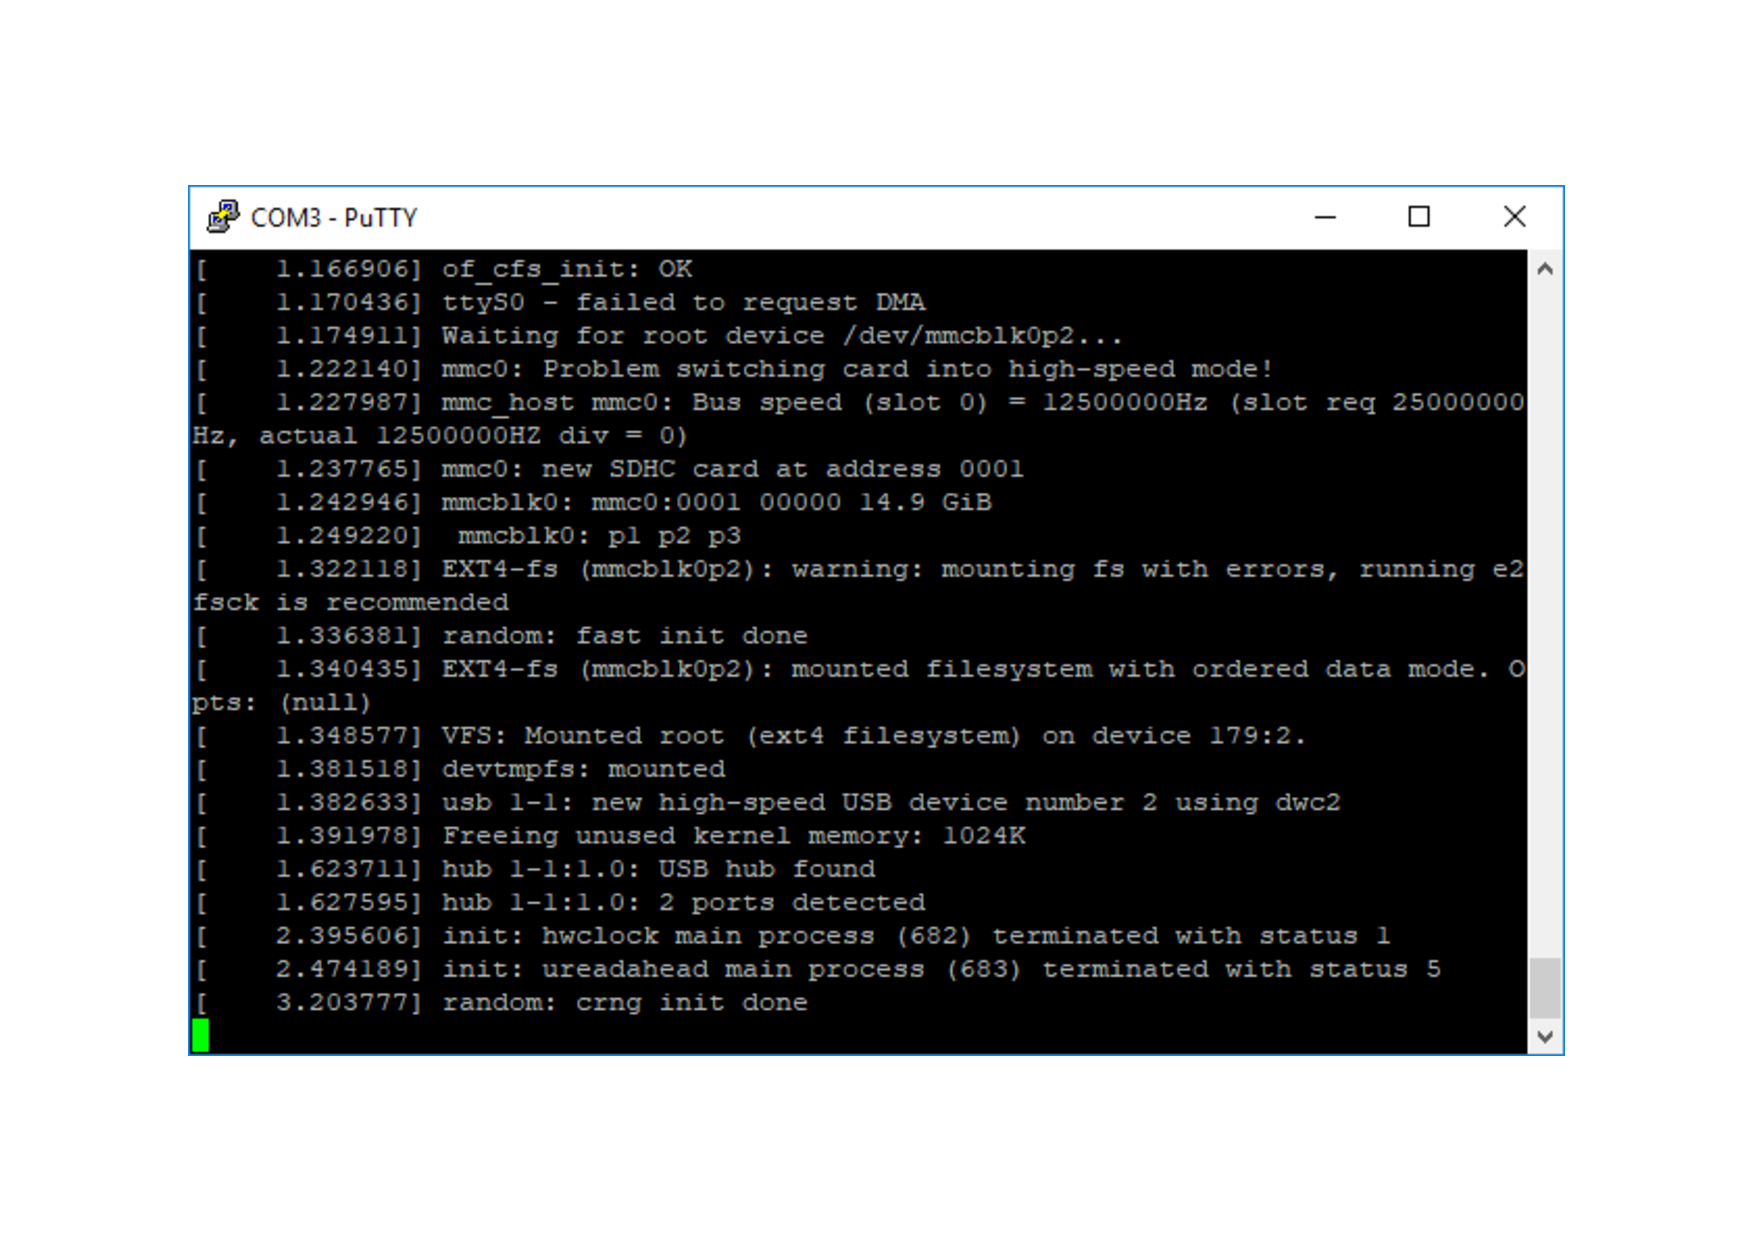
\includegraphics[width=1\linewidth]{images/putty_serial_connected}
%	\caption{Erfolgreich aufgebaute serielle Verbindung}
%	\label{fig:putty_serial_connected}
%\end{figure}
%
%
%\chapter{VNC Verbindung}
%
%Auf dem 
%%\begin{figure}[!htbp]
%%	\centering
%%	\begin{subfigure}{.5\textwidth}
%%		\centering¬
%%		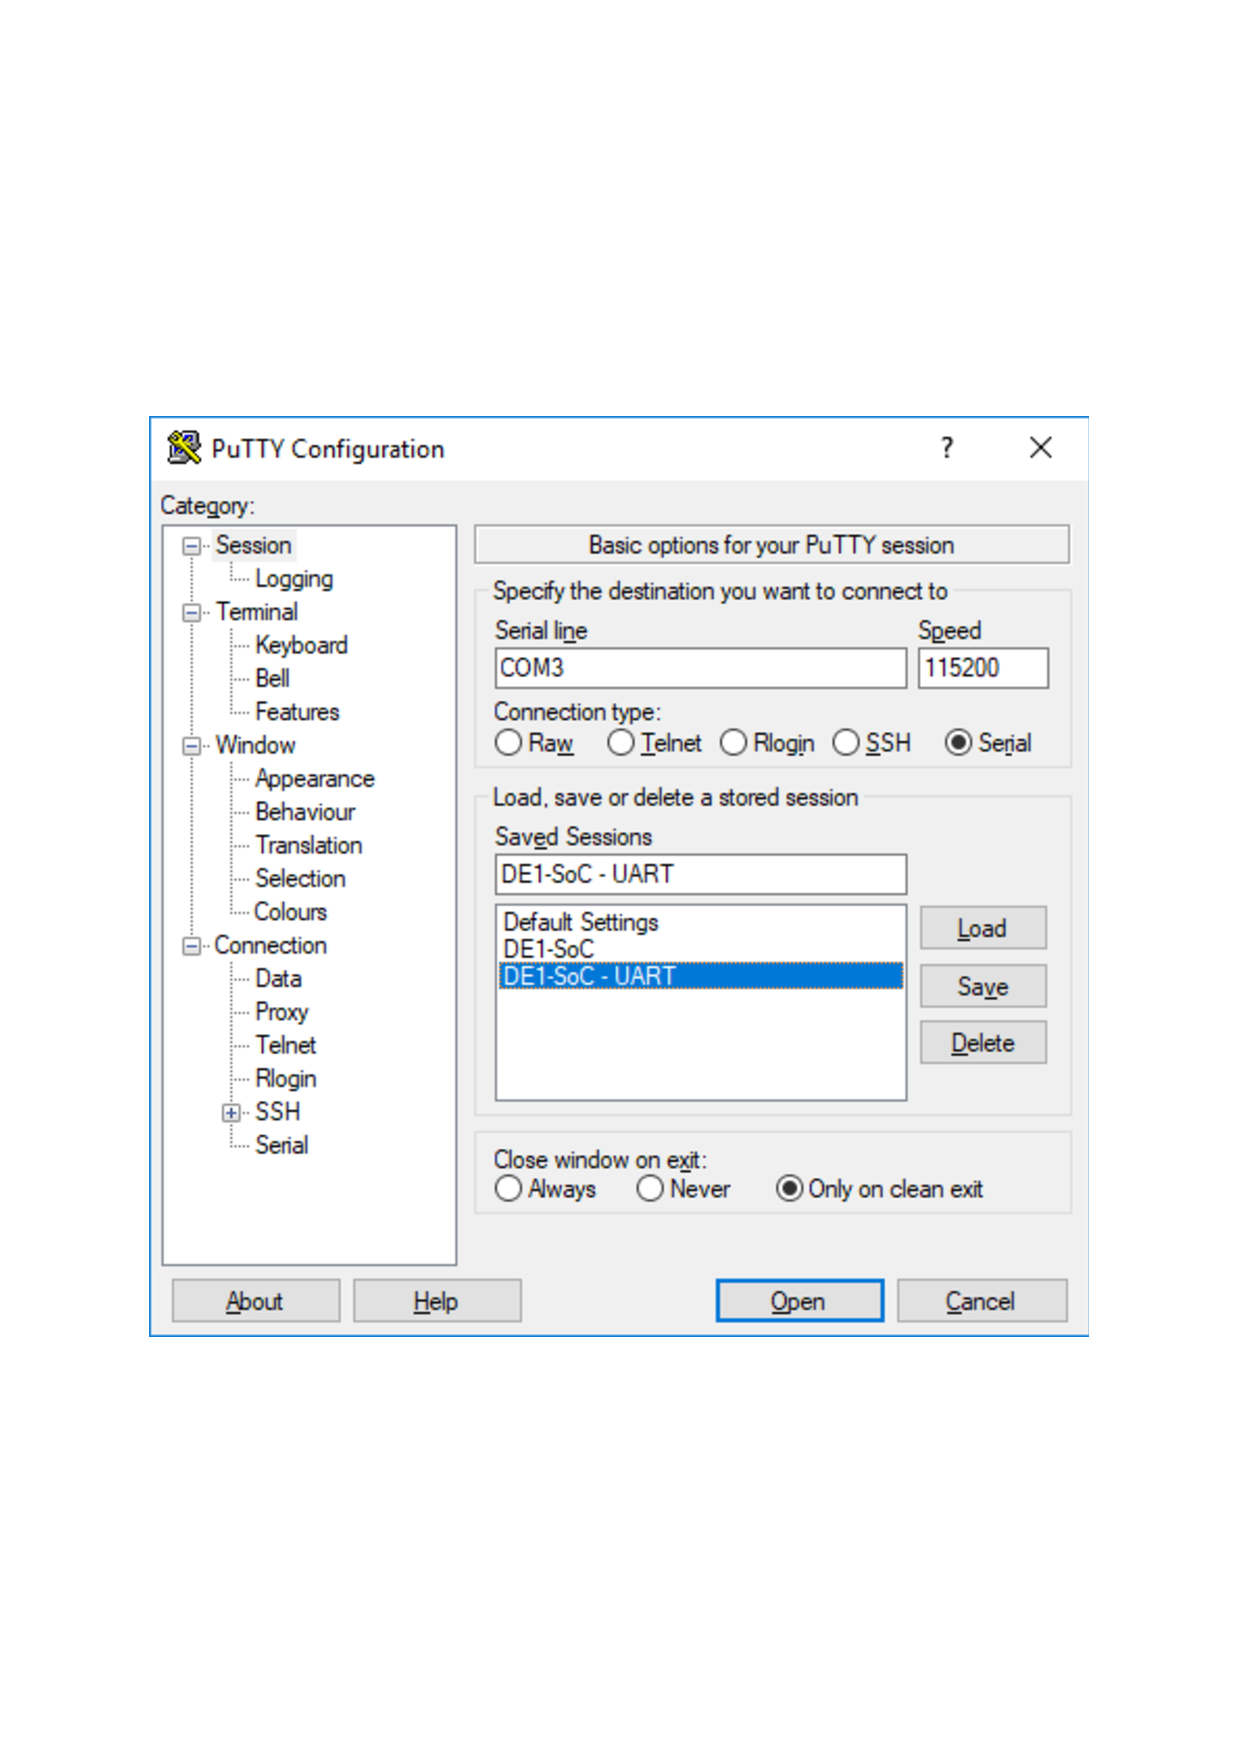
\includegraphics[width=0.9\linewidth]{images/putty_serial}
%%		\caption{Grundeinstellungen}
%%		\label{fig:putty_serial}
%%	\end{subfigure}%
%%	\begin{subfigure}{.5\textwidth}
%%		\centering
%%		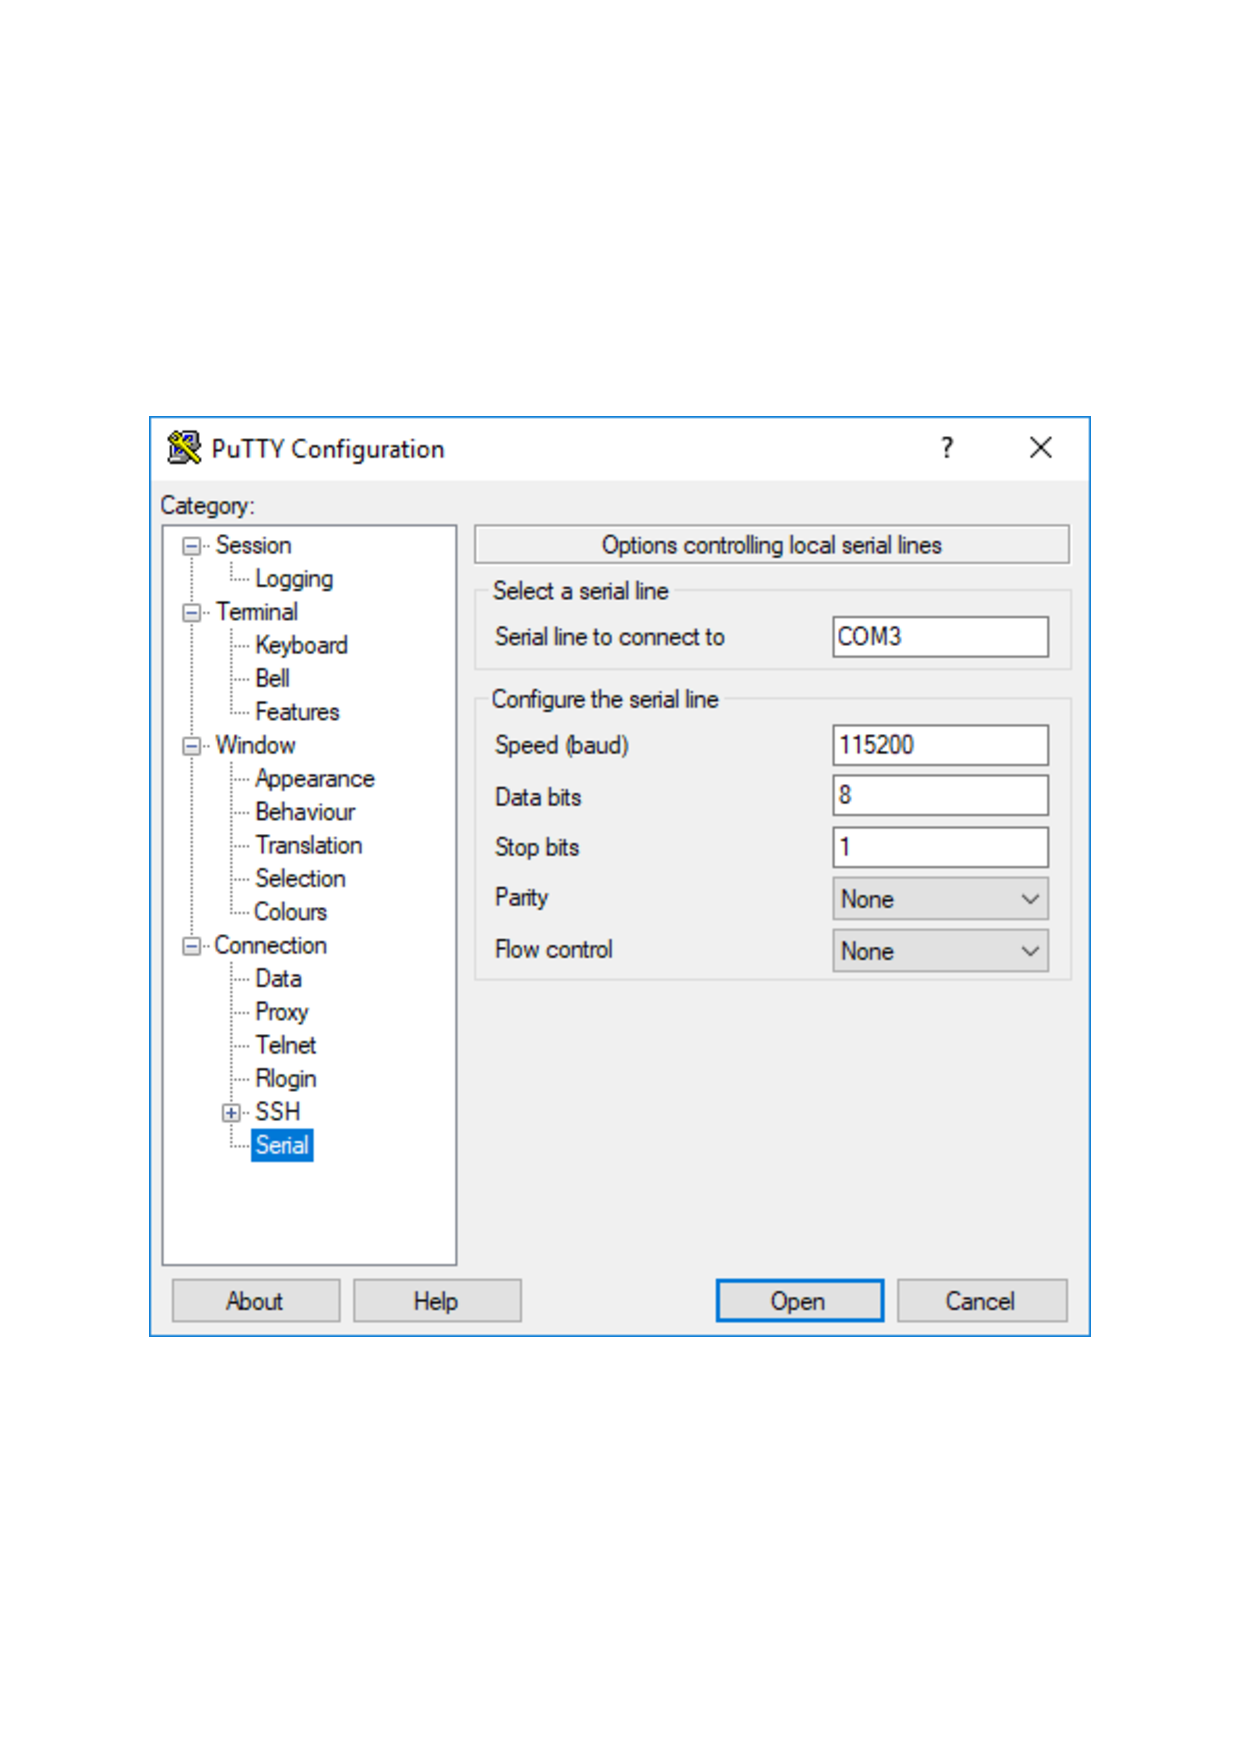
\includegraphics[width=0.9\linewidth]{images/putty_serial_params}
%%		\caption{Erweiterte Einstellungen}
%%		\label{fig:putty_serial_params}
%%	\end{subfigure}
%%	\caption{Putty-Konfiguration}
%%	\label{fig:putty}
%%\end{figure}
	%\chapter{Quelltexte}


\TeXOSQueryWalk{\vhdlfiles}{,}{.*\string\.vhd}{attachments/Plasma-Soc/}

\makeatletter
\ifx\vhdlfiles\empty
Query Failed!
\else
	\foreach \vhd in  \vhdlfiles {
		
		\inputminted[autogobble, breaklines=true]{VHDL}{attachments/Plasma-Soc/\vhd}
		\captionof{listing}{\textsf{\vhd} \label{lst:\vhd}}
	}
\fi
\makeatother	
	
\end{document}     